\documentclass[11pt,a4paper,twoside,openright]{book}
%\documentclass[a4paper,12pt,fourier,numbered,print,index]

% CHECK https://www.writelatex.com/1283488jybyzp#/3132576/
%%------------------------ PACKAGES------------------------------
%%------------------------ BOOLEANS FOR OPTIONS -------------------------------
\usepackage{ifthen}

\newboolean{enable_backrefs} % enable backrefs in the bibliography
\newboolean{enable_line_numbers}
\newboolean{enable_visual_comments}
\newboolean{enable_animations}
%%------------------------ CHOOSE COMPILATION OPTIONS (BOOLEANS) -------------------------------
\setboolean{enable_line_numbers}{false} 	% true false
\setboolean{enable_backrefs}{true} 			% true false
\setboolean{enable_visual_comments}{true} 	% true false
\setboolean{enable_animations}{true} 	% true false

\newcommand{\mycustomstyle}{References/customstyle} %path to .bst file for bibliography style

%%------------------------ General Info -------------------------------
\newcommand{\myTitle}{Modelling and Simulation of Macrosegregation Induced by Thermomechanical Deformation in Steels} %\xspace
%\newcommand{\mySubtitle}{\textsf{New} technique to solve \textsf{Old} problems !} %\xspace
\newcommand{\myDegree}{Ph.D.} %\xspace
\newcommand{\myName}{Ali SAAD } %\xspace
\newcommand{\myFaculty}{MINES ParisTech} %\xspace
\newcommand{\myDepartment}{Material Forming Center} %\xspace
\newcommand{\myUni}{PSL Research University}
\newcommand{\myLocation}{France}
\newcommand{\myDate}{December 2014}
\newcommand{\myVersion}{version 1.0}

%%------------------------ Classic Thesis Commands -------------------------------
%% Define \cleardoublepgage
%\makeatletter
%\def\cleardoublepage{\clearpage\if@twoside \ifodd\c@page\else
%    \hbox{}
%    \thispagestyle{empty}
%    \newpage
%    \if@twocolumn\hbox{}\newpage\fi\fi\fi}
%\makeatother \clearpage{\pagestyle{plain}\cleardoublepage}
%--------------------------------------------------------
%%------------------------ FONTS -------------------------------
%\usepackage{lmodern}
%\usepackage{fouriernc}
\usepackage{fourier} 		% Utopia font-typesetting including mathematical formula compatible with newer TeX-Distributions (>2010)
%\usepackage{utopia} 		% on older systems -> use this package instead of fourier in combination with mathdesign for better looking results
%\usepackage[adobe-utopia]{mathdesign}
%\usepackage{ae,aecompl}

%------------------------ LANGUAGES-FRENCH ACCENTS -------------------------------
\usepackage[utf8]{inputenc}
% For the front page
\usepackage[T1]{fontenc}		
\usepackage[francais, english]{babel} % american
%\usepackage{utopia} % lmodern % utopia % fourier

%%------------------------ ACRONYMS -------------------------------
%\usepackage[printonlyused,smaller]{acronym}
%\renewcommand{\bflabel}[1]{{#1}\hfill} % fix the list of acronyms

%%------------------------ BIBLIOGRAPHY NATBIB (deprecated) -------------------------------
% http://merkel.zoneo.net/Latex/natbib.php
% default option for citation rendering is "authoryear" and "round" brackets
% sort: orders multiple citations into the sequence in which they appear in the list of references;
% sort&compress: as sort but in addition multiple numerical citations are compressed if possible (as 3-6, 15);

%\usepackage[square,numbers]{natbib}    % number in square , useful to add sortcompress
%\usepackage[square,sort]{natbib} % name and year in square

%%------------------------ BIBLIOGRAPHY BIBLATEX -------------------------------
\usepackage{csquotes}% Recommended
\usepackage [backend=bibtex,style=authoryear]{biblatex} %style=authoryear %style=apa

% Rename citation commands (instead of redefining them, impossible then to use optional "see" or page number
\let\citep\parencite
\let\citet\textcite
% (deprecated)
%\newcommand{\citep}[1]{\parencite{#1}}
%\newcommand{\citet}[1]{\textcite{#1}}

\ExecuteBibliographyOptions{hyperref=true,
							backref=true,
							firstinits=true, 
							isbn=false, 
							eprint=false,
							url=true, 
							doi=false, 
							sorting=nyt, 
							minnames=1, 
							maxcitenames=1, % in text citations, allows suffix a,b ...
							maxbibnames=5,
							alldates=short, 
							punctfont=true, 
							autopunct=false, 
							block=none, 
							dashed=false}
% bibresource moved to "main.tex" to allow autcomplete in TexMaker
%\addbibresource{References/auto_references.bib}

% Spacing
\setlength{\bibitemsep}{10pt} %vertical spacing
\setlength{\bibhang}{1cm} %label alignment (0 for perfect align)

% Disable URL dates
\AtEveryBibitem{%
    \clearfield{urldate}%
    \clearfield{urlday}%
    \clearfield{urlmonth}%
    \clearfield{urlyear}%
    \clearlist{language}
}%

%Fix the comma problem after the journal name (via addcomma)
\DeclareFieldFormat{journaltitle}{\mkbibemph{#1\isdot}\addcomma\space}

%Fix number and volume format
\renewbibmacro*{volume+number+eid}{%
  \printfield{volume}%
%  \setunit*{\adddot}% DELETED
  \setunit*{\addnbspace}% NEW (optional); there's also \addnbthinspace
  \printfield{number}%
  \setunit{\addcomma\space}%
  \printfield{eid}}
\DeclareFieldFormat[article]{number}{\mkbibparens{#1}}

%Disable prefix "In"
\renewbibmacro{in:}{}

% Define brackets instead of parenthesis
\makeatletter
\newrobustcmd*{\parentexttrack}[1]{%
  \begingroup
  \blx@blxinit
  \blx@setsfcodes
  \blx@bibopenparen#1\blx@bibcloseparen
  \endgroup}
\AtEveryCite{%
  \let\parentext=\parentexttrack%
  \let\bibopenparen=\bibopenbracket%
  \let\bibcloseparen=\bibclosebracket}
\makeatother

%define label before reference in list	
\renewbibmacro{begentry}{%
\textbf{[\printnames[][-\value{liststop}]{labelname}~\printfield{labelyear}\printfield{extrayear}}]\\}

%define full hyperlink for textcite and parencite
% http://tex.stackexchange.com/questions/15951/hyperlink-name-with-biblatex-authoryear-biblatex-1-4b
\DeclareFieldFormat{citehyperref}{%
\DeclareFieldAlias{bibhyperref}{noformat}% Avoid nested links
\bibhyperref{#1}}
\DeclareFieldFormat{textcitehyperref}{%
\DeclareFieldAlias{bibhyperref}{noformat}% Avoid nested links
\bibhyperref{%
#1%
\ifbool{cbx:parens}
  {\bibcloseparen\global\boolfalse{cbx:parens}}
  {}}}
\savebibmacro{cite}
\savebibmacro{textcite}

\renewbibmacro*{cite}{%
\printtext[citehyperref]{%
\restorebibmacro{cite}%
\usebibmacro{cite}}}

\renewbibmacro*{textcite}{%
\ifboolexpr{
( not test {\iffieldundef{prenote}} and
  test {\ifnumequal{\value{citecount}}{1}} )
or
( not test {\iffieldundef{postnote}} and
  test {\ifnumequal{\value{citecount}}{\value{citetotal}}} )
}
{\DeclareFieldAlias{textcitehyperref}{noformat}}
{}%
\printtext[textcitehyperref]{%
\restorebibmacro{textcite}%
\usebibmacro{textcite}}}

%%------------------------ LAYOUT -------------------------------

% Package geometry is loaded ONLY to achieve a specific size in title page (SHOULD BE LOADED BEFORE CUSTOM LAYOUT SETTINGS)
\usepackage[top=1cm, bottom=1cm, left=1cm, right=1cm, headheight=15pt]{geometry}

%% --- Margins (Custom layout)
\setlength{\textwidth}{146.8mm} % = 210mm - 37mm - 26.2mm
\setlength{\oddsidemargin}{11.6mm} % 37mm - 1in (from hoffset)
\setlength{\evensidemargin}{0.8mm} % = 26.2mm - 1in (from hoffset)
\setlength{\topmargin}{-2.2mm} % = 0mm -1in + 23.2mm 
\setlength{\textheight}{221.9mm} % = 297mm -29.5mm -31.6mm - 14mm (12 to accomodate footline with pagenumber)
\setlength{\headheight}{14pt}
%% --- Paragraph spacing
\setlength{\parindent}{0pt}
%% --- Interline spacing
\usepackage{setspace} % increase interline spacing slightly
\setstretch{1.1}

%%------------------------ Captions  -------------------------------

% Captions: This makes captions of figures use a boldfaced small font. 
\RequirePackage[small,bf]{caption}
\RequirePackage[labelsep=endash,tableposition=top]{caption}  % labelsep=endash % space
\addto\captionsenglish{\renewcommand{\figurename}{Fig.}}

%%-----------------------  Footnote Header formatting -------------------------------
% From EPFL template
%\usepackage[perpage]{footmisc} %Range of footnote options 

\usepackage{fancyhdr}
\renewcommand{\sectionmark}[1]{\markright{#1}}  %\markright{\thesection\ #1}
\pagestyle{fancy}
	\fancyhf{}
	\renewcommand{\headrulewidth}{0.4pt}
	\renewcommand{\footrulewidth}{0pt}
	\fancyhead[OR]{\bfseries \nouppercase{\rightmark}}
	\fancyhead[EL]{\bfseries \nouppercase{\leftmark}}
	\fancyfoot[EL,OR]{\thepage}
\fancypagestyle{plain}{
	\fancyhf{}
	\renewcommand{\headrulewidth}{0pt}
	\renewcommand{\footrulewidth}{0pt}
	\fancyfoot[EL,OR]{\thepage}}
\fancypagestyle{addpagenumbersforpdfimports}{
	\fancyhead{}
	\renewcommand{\headrulewidth}{0pt}
	\fancyfoot{}
	\fancyfoot[RO,LE]{\thepage}
}

%%------------------------ Figures  -------------------------------
%\usepackage{rotating}
%\usepackage{wrapfig}
%\usepackage{float}
%\usepackage{subfig} %note: subfig must be included after the `caption` package.
\usepackage{subcaption}
 

% \usepackage{graphicx,xcolor}
\usepackage[dvipsnames]{xcolor}
\definecolor{webgreen}{rgb}{0,.5,0}
\definecolor{webbrown}{rgb}{.6,0,0}
\definecolor{Maroon}{cmyk}{0, 0.87, 0.68, 0.32}
\definecolor{RoyalBlue}{cmyk}{1, 0.50, 0, 0}

%\graphicspath{{images/}}
\makeatletter
\setlength{\@fptop}{0pt}  % for aligning all floating figures/tables etc... to the top margin
\makeatother

%%------------------------ Tables  -------------------------------
%\usepackage{longtable}
%\usepackage{multicol}
%\usepackage{multirow}
%\usepackage{tabularx}

%\usepackage{booktabs}

%%------------------------ Math and SI Units  -------------------------------
\usepackage{amsfonts}
\usepackage{amsmath}
\usepackage{amssymb}
\usepackage[mathscr]{euscript}
\usepackage{siunitx} % http://ftp.oleane.net/pub/CTAN/macros/latex/contrib/siunitx/siunitx.pdf
% \num{.3e45}   ,  \num{3.45d-4}   , \numlist{10;30;50;70} ,  \numrange{10}{30} , 

%%------------------------ Cross References  -------------------------------
% --- Hyperref and Options
\usepackage{hyperref}
\hypersetup{%
	% --------------
	% PDF Display
	% --------------
    linktocpage=false, % make page number, not text, be link on TOC, LOF and LOT
    linktoc=all,
    pdfstartpage=1, 
    pdfstartview=FitV, % FitR (rectangle) % FitH %FitV % FitB (bounding box) % FitBH % FitBV
    %
    breaklinks=true, 
    pageanchor=true,  % put an anchor on every page, DO NOT TURN OFF
    pdfpagemode=UseOutlines,  % UseNone % UseOutlines (shows bookmarks) % UseThumbs
    plainpages=false, % Forces page anchors to be named by the Arabic form of the page number, rather than the formatted form.
	%
    bookmarksnumbered, 
    bookmarksopen=false, 
    bookmarksopenlevel=3,%
	pdfpagelayout=TwoPageRight,  % SinglePage % TwoPageLeft % TwoPageRight
	hypertexnames=true, % use guessable names for links, DO NOT TURN OFF
    pdfhighlight=/O, % How link buttons behave when selected; /I is for inverse (the default) /N (no effect), /O (outline), and /P (inset highlighting).
	%
	% --------------
	% Hyperlink Colors
	% --------------  
	colorlinks=true,  
    urlcolor=webbrown, %webbrown %Black
    linkcolor=RoyalBlue, %RoyalBlue, %Black
    citecolor=webgreen, %webgreen, %Black
    pagecolor=RoyalBlue,%Black
	% --------------
    % PDF Information
	% --------------  
    pdftitle={\myTitle},%
    pdfauthor={\myName, \myUni, \myFaculty},%
    pdfkeywords={Macrosegregation, solidification, level set, numerical simulation}%
}


%% --- cleveref (should always be invoked AFTER hyperref)
%\usepackage{cleveref}
\usepackage[nameinlink]{cleveref} % capitalize


\DefineBibliographyStrings{english}{%
  backrefpage = {cited on page},% originally "cited on page"
  backrefpages = {cited on pages},% originally "cited on pages"
}

%% --- beckref and Options (NATBIB compatible - Obsolete)
%\newcommand{\backrefnotcitedstring}{\relax}%(Not cited.)
%\newcommand{\backrefcitedsinglestring}[1]{(cited on page~#1)}
%\newcommand{\backrefcitedmultistring}[1]{(cited on pages~#1)}
%\ifthenelse{\boolean{enable_backrefs}}%
%{%
%		\usepackage[hyperpageref]{backref}  % to be loaded after hyperref package
%		   \renewcommand{\backreftwosep}{ and~} % separate 2 pages
%		   \renewcommand{\backreflastsep}{, and~} % separate last of longer list
%		   \renewcommand*{\backref}[1]{}  % disable standard
%		   \renewcommand*{\backrefalt}[4]{% detailed backref
%		      \ifcase #1 %
%		         \backrefnotcitedstring%
%		      \or%
%		         \backrefcitedsinglestring{#2}%
%		      \else%
%		         \backrefcitedmultistring{#2}%
%		      \fi}%
%}%{\relax}    

%%--------------------- TOC --------
%\setcounter{secnumdepth}{2}
%\setcounter{tocdepth}{2}

\usepackage{minitoc} % use like this : \minitoc 
\setcounter{minitocdepth}{2}
\setlength{\mtcindent}{24pt} 
\renewcommand{\mtcfont}{\small\rm}
\renewcommand{\mtcSfont}{\small\bf}


%%------------------------ NOMENCLATURE / GLOSSARY -------------------------------
% http://www.latex-community.org/know-how/latex/55-latex-general/263-glossaries-nomenclature-lists-of-symbols-and-acronyms
%\usepackage[toc]{glossaries}
% use it like: \newglossaryentry{label}{definition}
%\usepackage[xindy,toc]{glossaries}  
%\makeglossaries 


%%------------------------ Names of sections for figures, nomenclature ...  -------------------------------
% To change the name of the Nomenclature section, uncomment the following line
%\renewcommand{\contentsname}{My Table of Contents}
%\renewcommand{\listfigurename}{My List of Figures}
%\renewcommand{\listtablename}{My List of Tables}
%\renewcommand{\nomname}{Symbols}

%%------------------------ Appendix -------------------------------
\usepackage[titletoc]{appendix}
% The default value of both \appendixtocname and \appendixpagename is `Appendices'. These names can all be changed via: 
%\renewcommand{\appendixtocname}{List of appendices}
\renewcommand{\appendixname}{Appendicitis}

%%------------------------ MISC PACKAGES -------------------------------
% Graphs
\usepackage{pgfplots}
\pgfplotsset{width=8cm,compat=newest}
%\usepgfplotslibrary{external}
%\tikzexternalize

% Format URLs
\usepackage{url}

% Input dummy text
\usepackage{lipsum}

\usepackage{pdfpages} %\includepdf[options]{filename}
%\usepackage{algpseudocode} 

% Display line number
\usepackage{lineno}
\ifthenelse{\boolean{enable_line_numbers}}%
{%
	%\linenumbers
	\pagewiselinenumbers % requires compiling AT LEAST twice
}{\relax}    

% Comments
\usepackage{todonotes}
\ifthenelse{\boolean{enable_visual_comments}}%
{% then
   \newcommand{\comment}[2][]{\todo[backgroundcolor=yellow!50!white, caption={#2}, inline, size=\small, #1]{\renewcommand{\baselinestretch}{0.5}\selectfont#2\par}}
}
{% else 
  \newcommand{\comment}[2][]{}
}

% Enchance syllable breaking avoiding bad boxes
\usepackage[stretch=10]{microtype} % which allows font expansion up to 1% (default is 2%)

% Cancel sign in math equations
\usepackage{cancel}

% Enables putting the pdf_tex graphics in a subfolder
\usepackage{import}

% Frontpage packages (Dorian)
\usepackage{eso-pic}	% Nécessaire pour mettre des images en arrière plan
%\usepackage[top=1cm, bottom=1cm, left=1cm, right=1cm, headheight=15pt]{geometry}
%\usepackage{graphicx}
%\usepackage{array}		% Permet d'écrite 'THESE' de haut en bas


%%------------------------ ENVIRONMENTS  -------------------------------
% Change hyperlink color to black in miniTOC, TOC, TOF ...
\newenvironment{nolinkcolors}[1]{\begingroup \hypersetup{hidelinks}  #1 }{\endgroup}

%% Dorian Depriester: Figures centrées, et en position 'here, top, bottom or page'
\newenvironment{figureth}[3]{
		\begin{figure}[htbp]
			\centering
			\includegraphics[width=#1\textwidth]{#2}
			\caption{#3}
			%\label{fig:#4}
	}{
		\end{figure}
		}

% USE LIKE THIS	
%\begin{figureth}
% textwidth 
%{•}
%path 
%{•}
% caption
%{•}
% label
%{•}
%\end{figureth}

\newenvironment{figurethmulti}{
		\begin{figure}[htbp]
			\centering
	}{
		\end{figure}
		}

%**********
%% Tableaux centrés, et en position 'here, top, bottom or page'
\newenvironment{tableth}{
		\begin{table}[htbp]
			\centering
			
	}{
		\end{table}
		}
%**********	
\newenvironment{subfigureth}[2]{
		\begin{subfigure}[t]
			\centering
			\includegraphics[width=#1\textwidth]{#2}
			%\caption{#3}
			%\label{fig:#4}
	}{
		\end{subfigure}
		}
%**********	

%%------------------------ SI units -------------------------------
\DeclareSIUnit\udensity{\kilo \gram \per \cubic \metre}
\DeclareSIUnit\uacceleration{\metre \per \square \second}
\DeclareSIUnit\uvelocity{\metre \per \second}
\DeclareSIUnit\uviscosity{\pascal \second}
\DeclareSIUnit\ubetaT{\per \kelvin}
\DeclareSIUnit\ubetawl{\per \ucomposition}
\DeclareSIUnit\udiffusivity{\metre \squared \per \second}
\DeclareSIUnit\uconductivity{\watt \per \metre \per \kelvin}
\DeclareSIUnit\uhconvec{\watt\per \square \metre \per \kelvin}
\DeclareSIUnit\umasscapacity{\joule \per \kilo\gram \per \kelvin}
\DeclareSIUnit\umassenergy{\joule \per \kilo\gram}
\DeclareSIUnit\uvolumecapacity{\joule \per \cubic \metre \per \kelvin}
\DeclareSIUnit\uvolumeenergy{\joule \per \cubic \metre}
\DeclareSIUnit\udegC{\degreeCelsius}
\DeclareSIUnit\udegK{\kelvin}
\DeclareSIUnit\uCR{\kelvin \per \second}

\DeclareSIUnit\ucomposition{wt.\%}  % used in tables
\DeclareSIUnit\uslope{\udegK \per \ucomposition}  % used in tables
\newcommand\bin[3]{#1-\SI{#2}{\ucomposition} #3}	% used in text
\newcommand\tern[5]{#1-\SI{#2}{\ucomposition} #3-\SI{#4}{\ucomposition} #5} % used in text

%% ------------------------ MATHs commands--------------------------
%\renewcommand{matrix}[1]{#1 \rangle} 
\newcommand{\avg}[1]{\ensuremath{\langle  #1 \rangle}}
\newcommand{\brac}[1]{\ensuremath{\left(  #1 \right)}} 
\newcommand{\curly}[1]{\ensuremath{\left\{  #1 \right\}}}
\newcommand{\crochet}[1]{ \left[  #1  \right] } 
\newcommand{\abval}[1]{\ensuremath{\left |  #1 \right |}} 
\newcommand\norm[1]{\ensuremath{\lVert #1 \rVert}}

\renewcommand\d{\ensuremath{\partial}}
\newcommand\integral[3]{\ensuremath{\int_{#1} #2\: \mathrm{d}#3}}
\newcommand{\deriv}[1]{\frac{\partial #1 }{\partial t}}
\newcommand{\diff}[2]{ \ensuremath{\nabla \cdot \brac{ #1 \nabvec #2}}}

%\newcommand{\mtrx}[1]{{\underline{\underline{#1}}} }
\newcommand{\mtrx}[1]{{\overline{\overline{#1}}} }
\newcommand{\mat}[1]{{\overline{\overline{#1}}} }


\newcommand\hilbert{\ensuremath{\mathscr{H}^1}}
\newcommand\order{\ensuremath{\mathscr{O}}}
\newcommand\test{\ensuremath{\mathscr{W}}}
\newcommand\interp{\ensuremath{\mathscr{P}}}
\newcommand\Mij{\ensuremath{\mathscr{M}_{ij}}}
\newcommand\Aij{\ensuremath{\mathscr{A}_{ij}}}
\newcommand\Kija{\ensuremath{\mathscr{K}1_{ij}}} % diffusion term
\newcommand\Kijb{\ensuremath{\mathscr{K}2_{ij}}} % boundary condition
\newcommand\Fi{\ensuremath{\mathscr{F}_{i}}}
\newcommand\Si{\ensuremath{\mathscr{S}_{i}}}
\newcommand\Ohm{\ensuremath{\Omega}}
\newcommand\dOhm{\ensuremath{\partial \Ohm}}
\newcommand\OhmE{\ensuremath{\Ohm_E}}
\newcommand\dOhmE{\ensuremath{\partial \OhmE}}
\newcommand\element{\ensuremath{\Ohm_E}}
%--------------------------
\newcommand\itersymbol{\nu}
%--------------------------
\newcommand\iter{\ensuremath{{\brac{\itersymbol}}}}
\newcommand\iterplus{\ensuremath{{\brac{\itersymbol+1}}}}
\newcommand\iterminus{\ensuremath{{\brac{\itersymbol-1}}}}
\newcommand\dRdH{\ensuremath{\frac{dR}{dH}}}
\newcommand\dRdT{\ensuremath{\frac{dR}{dT}}}
\newcommand\dTdH{\ensuremath{\frac{dT}{dH}}}
\newcommand\dTdHjt{\ensuremath{\brac{dT/dH}_j^{t}}}
\newcommand\dTdHjk{\ensuremath{\brac{dT/dH}_j^{\iter}}}
\newcommand\dTdHjkplus{\ensuremath{\brac{dT/dH}_j^{\iterplus}}}
\newcommand\dHdT{\ensuremath{\frac{dH}{dT}}} 
\newcommand\dHdTjk{\ensuremath{\brac{dH/dT}_j^{\iter}}}
\newcommand\dHdTjkplus{\ensuremath{\brac{dH/dT}_j^{\iterplus}}}
\newcommand\dHdTjt{\ensuremath{\brac{dH/dT}_j^{t}}}
\newcommand\dRdTijk{\ensuremath{\brac{\frac{dR}{dT}}_{ij}^{\iter}}}
\newcommand\dRdHijk{\ensuremath{\brac{\frac{dR}{dH}}_{ij}^{\iter}}}
\newcommand\Rjk{\ensuremath{R_{j}^{\iter}}}

\newcommand\nabvec{\ensuremath{\vec{\nabla}}}
\newcommand\nabmat{\ensuremath{\mat{\nabla}}}
\newcommand\nabmattransp{\ensuremath{\mat{\nabla^\text{t}}}}
\newcommand\temp[1]{\ensuremath{\frac{\partial}{\partial t} \brac{#1} }} 
\newcommand\tempup[1]{\ensuremath{\frac{\partial #1}{\partial t} }} 
\newcommand\vit{\ensuremath{\avg{\vec{v^l}}}}  
\newcommand\vitf{\ensuremath{\avg{\vf}}}
\newcommand\vita{\ensuremath{\avg{\va}}}
\newcommand\strainrate{\ensuremath{\avg{\mat{\dot{\varepsilon}^l}}}}
\newcommand\I{\ensuremath{\mat{\mathrm{I}}}}  

%TODO :redundant defnitions rh and rhoh
%TODO :redundant defnitions rhv and rhohv
\renewcommand\r{\ensuremath{\avg{ \rho }}}
\newcommand\rl{\ensuremath{\avg{ \rho }^l}}
\newcommand\h{\ensuremath{\avg{ h }}}
\newcommand\rh{\ensuremath{\avg{ \rho h }}}
\newcommand\rhoh{\ensuremath{\avg{ \rho h }}}
\newcommand\rhv{\ensuremath{\avg{ \rho h \vec{v} }}}
\newcommand\rhohv{\ensuremath{\avg{ \rho h \vec{v} }}}
\newcommand\rcp{\ensuremath{\avg{ \rho C_p }}}

\newcommand\w{\ensuremath{\avg{w}}}
\newcommand\wi{\ensuremath{\avg{w_i}}}
%\newcommand\wil{\ensuremath{\avg{w_i}^l}}
\newcommand\wil{\ensuremath{w_i^l}}
\newcommand\wis{\ensuremath{w_i^s}}
\newcommand\gphi{\ensuremath{{g^{\phi}} }}
\newcommand\wiphi{\ensuremath{\wi^\phi}}
\newcommand\rphi{\ensuremath{\rho^{\phi} }}
\newcommand\hphi{\ensuremath{h^{\phi} }}
\newcommand\Tk{\ensuremath{T^\iter}}
\newcommand\Tkplus{\ensuremath{T^\iterplus}}
\newcommand\Tkinit{\ensuremath{T^{\brac{k=0}}}}
\newcommand\Hk{\ensuremath{\rh^{\brac{k}}}}
\newcommand\Hkinit{\ensuremath{\rh^{\brac{k=0}}}}
\newcommand\source{\ensuremath{\avg{\dot{Q}_{{V}}}}}
\newcommand\Hj{\ensuremath{H_j}}
\newcommand\Hjt{\ensuremath{H_j^t}}
\newcommand\Hjk{\ensuremath{H_j^\iter}}
\newcommand\Hjkminus{\ensuremath{H_j^{\iterminus}}}
\newcommand\Hjkplus{\ensuremath{H_j^{\iterplus}}}
\newcommand\Hjtminus{\ensuremath{H_j^{t-\dt}}}
\newcommand\Hjtplus{\ensuremath{H_j^{t+\dt}}}
\newcommand\Tj{\ensuremath{T_j}}
\newcommand\Tjt{\ensuremath{T_j^t}}
\newcommand\Tjk{\ensuremath{T_j^\iter}}
\newcommand\Tjkminus{\ensuremath{T_j^{\iterminus}}}
\newcommand\Tjkplus{\ensuremath{T_j^{\iterplus}}}
\newcommand\Tjtminus{\ensuremath{T_j^{t-\dt}}} 
\newcommand\Tjtplus{\ensuremath{T_j^{t+\dt}}} 
\newcommand\nosum{\text{no sum on }j} 

%TODO :redundant defnitions rhoref and rref
\newcommand\rhoref{\ensuremath{\rho_{\text{ref}}}}
\newcommand\rref{\ensuremath{\rho_{\text{ref}}}}
\newcommand\rholref{\ensuremath{\rho_{0}^{l}}}
\newcommand\Tref{\ensuremath{T_{0}}}
\newcommand\wlref{\ensuremath{w_{0}^l}}
\newcommand\wilref{\ensuremath{\wi_{0}^l}}
\newcommand\betaT{\ensuremath{\beta_T}}
\newcommand\betawl{\ensuremath{\beta_{\wl}}}
\newcommand\betawil{\ensuremath{\beta_{\wil}}}
\newcommand\betawlC{\ensuremath{\beta_{\avg{w_\text{C}}^l}}}
\newcommand\betawlCR{\ensuremath{\beta_{\avg{w_\text{Cr}}^l}}}

\newcommand\wavg{\ensuremath{\avg{w}}}
\newcommand\wC{\ensuremath{\avg{w_\text{C}}}}
\newcommand\wCR{\ensuremath{\avg{w_\text{Cr}}}}
\newcommand\wl{\ensuremath{\avg{w}^l}}
\newcommand\ws{\ensuremath{\avg{w}^s}}
\newcommand\wa{\ensuremath{\avg{w}^A}}
\newcommand\Cnominal{\ensuremath{{w}_0}}
\newcommand\Cl{\ensuremath{{w}^l}}
\newcommand\Clstar{\ensuremath{{w}^{l \text{*}} }}
\newcommand\Cs{\ensuremath{{w}^s}}
\newcommand\Csstar{\ensuremath{{w}^{s \text{*}} }}

\renewcommand\k{\ensuremath{k}}
\newcommand\ml{\ensuremath{{m}^l}}
\newcommand\ms{\ensuremath{{m}^s}}
\newcommand\pdas{\ensuremath{{\lambda}_{1}}}
\newcommand\sdas{\ensuremath{{\lambda}_{2}}} 
\newcommand\Tcoh{\ensuremath{{T}_{\text{coh}}}} 
\newcommand\Fos{\ensuremath{\text{Fo}^s}} % Fourier number in the solid
\newcommand\tsolidif{\ensuremath{t_\text{s}}} % solidification time in Fourier number 
\newcommand\rev{\ensuremath{V_\text{E}}} % V_\text{RVE}
\newcommand\Vs{\ensuremath{V^s}}
\newcommand\Vl{\ensuremath{V^l}}
\newcommand\Vphi{\ensuremath{V^\phi}}
\newcommand\psis{\ensuremath{\avg{\psi}^s}}
\newcommand\psil{\ensuremath{\avg{\psi}^l}}
\newcommand\gammastar{\ensuremath{{\Gamma}^{\text{*}} }}

\newcommand\rhof{\ensuremath{\rho^F}}
\newcommand\rhoa{\ensuremath{\rho^A}}
\newcommand\rhol{\ensuremath{\rho^l}}
\newcommand\rhos{\ensuremath{\rho^s}}
\newcommand\rhov{\ensuremath{\avg{\rho \vec{v}}}}
\newcommand\rholvl{\ensuremath{\rho^l \vl}}
\newcommand\rhosvs{\ensuremath{\rho^s \vs}}
\newcommand\cpl{\ensuremath{C_p^l}}
\newcommand\cps{\ensuremath{C_p^s}}
\newcommand\cpa{\ensuremath{C_p^A}}
\newcommand\kl{\ensuremath{\avg{\kappa^l}}}  % I added \avg
\newcommand\ks{\ensuremath{\avg{\kappa^s}}}	 % I added \avg
\newcommand\hf{\ensuremath{h^F}}
\newcommand\ha{\ensuremath{h^A}}
\newcommand\hl{\ensuremath{h^l}}
\newcommand\hs{\ensuremath{h^s}}
\newcommand\gf{\ensuremath{{g^F}}} % double braces useful for additional superscripts
\newcommand\ga{\ensuremath{{g^A}}} % double braces useful for additional superscripts
\newcommand\gl{\ensuremath{{g^l}}} % double braces useful for additional superscripts
\newcommand\gs{\ensuremath{{g^s}}} % double braces useful for additional superscripts
\newcommand\fl{\ensuremath{{f^l}}} % double braces useful for additional superscripts
\newcommand\fs{\ensuremath{{f^s}}} % double braces useful for additional superscripts
\newcommand\pf{\ensuremath{{p^F}}}
\newcommand\pl{\ensuremath{{p^l}}}
\newcommand\ps{\ensuremath{p^s}}
\newcommand\Da{\ensuremath{D^A}}
\newcommand\Dl{\ensuremath{D^l}}
\newcommand\Ds{\ensuremath{D^s}}
\newcommand\Dphi{\ensuremath{D^\phi}}
\newcommand\mul{\ensuremath{\mu^l}}
\newcommand\mus{\ensuremath{\mu^s}}
\newcommand\K{\ensuremath{\mathbb{K}}} %permeability
\newcommand\sigmal{\ensuremath{\mat{\sigma^l}}}
\newcommand\sigmas{\ensuremath{\mat{\sigma^s}}}

\newcommand\vf{\ensuremath{\vec{v^F}}}
\newcommand\va{\ensuremath{\vec{v^A}}}
\newcommand\vl{\ensuremath{\vec{v^l}}}
\newcommand\vs{\ensuremath{\vec{v^s}}}
\newcommand\vphi{\ensuremath{\vec{v}^\phi}}
\newcommand\vstar{\ensuremath{\vec{v}^\text{*}}}
\newcommand\vlstar{\ensuremath{\vec{v}^{l \text{*}}}}
\newcommand\vsstar{\ensuremath{\vec{v}^{s \text{*}}}}

\newcommand\gravity{\ensuremath{\vec{g}}}

\newcommand\dt{\ensuremath{\Delta t}}
\newcommand\hext{\ensuremath{h_{\text{ext}}}}
\newcommand\Text{\ensuremath{T_{\text{ext}}}}

\newcommand*\widefbox[1]{\fbox{\hspace{2em}#1\hspace{2em}}}

% From "Mixing Boussinesq" report
%\renewcommand\v{\ensuremath{\vec{v}}}  
\newcommand\Fv{\ensuremath{\vec{F}_{\text{v}}^l}}  
\newcommand\rhog{\ensuremath{\rho \vec{g}}}  
\newcommand\rhobouss{\ensuremath{\widetilde{\rho}}} 
\newcommand\heaviside{\ensuremath{H}}  
\newcommand{\heavisideM}{ \ensuremath{\heaviside^M}}
\newcommand{\heavisideA}{ \ensuremath{\heaviside^A}}
\newcommand\dirac{\ensuremath{\delta \brac{\levelset}}}
\newcommand\levelset{\ensuremath{\alpha}}
\newcommand\levelsettest{\ensuremath{\alpha^\text{*}}}
\newcommand\levelsetx{\ensuremath{\levelset \brac{\vec{x}}}}
\newcommand{\mix}[1]{\ensuremath{\widehat{#1}}} % \widehat % \overbrace % \widetilde

% Common nouns and names
\newcommand{\registered}{\textsuperscript{\textregistered}}
\newcommand{\cimlib}{\emph{CimLib }}
\newcommand{\thercast}{\emph{Thercast\registered }}
\newcommand{\ccemlcc}{\emph{CCEMLCC }} 
\newcommand{\doitpoms}{\emph{© DoITPoMS, University of Cambridge}} 
\newcommand\HtoT{\emph{H2T }}
\newcommand\TtoH{\emph{T2H }}


% Colors
\newcommand{\red}[1]{{\color{Red} #1}}
\newcommand{\blue}[1]{{\color{Blue} #1}} 

% List of acronyms
\usepackage{tabu}

\newcommand{\listofacronyms}{
\cleardoublepage
%-----------------------------
{\tabulinesep=1.5mm
\begin{tabu}{p{2cm} p{12cm}}
\tabucline[1pt]{-}
\textbf{Acronym} & 	\textbf{Standing for} \\\tabucline[1pt]{-}
%-----------------------------
ALE		&	Arbitrary Lagrangian-Eulerian \\
CCEMLCC & 	Chill Cooling for the Electro-Magnetic Levitator in relation with Continuous Casting of steel \\
CEMEF 	& 	Center for Material Forming \\
% CSF
DLR		&	Deutsches Zentrum für Luft- und Raumfahrt  \\
EML 	& 	Electromagnetic levitation 	\\
ESA 	& 	European Space Agency 		\\
FEM 	& 	Finite Element Method \\
%gas metal arc welding
ISS 	&	International Space Station \\
IWT		&	Institut für Werkstofftechnik \\
LHS		& 	Left Hand Side\\ 
% level set method
MAC		&	Marker-and-cell \\
PF		&	Phase field \\
RHS		& 	Right Hand Side\\ 
RUB		& 	Ruhr Universität Bochum \\ 
RVE		&	Representative Elementary Volume\\
VOF		&	Volume Of Fluid					\\\tabucline[1pt]{-}
%-----------------------------
\end{tabu}}
}
%%%%%%%%%%%%%%%%%%%%%%%%%%%%%%%%%%%%%%%%
%           Page de garde              %
%%%%%%%%%%%%%%%%%%%%%%%%%%%%%%%%%%%%%%%%
% Dorian Depriester (dorian.depriester@mines-paristech.fr), 2014
% Ali Saad 			(ali.saad@mines-paristech.fr), 			2015

\makeatletter
\def\@ecole{école}
\newcommand{\ecole}[1]{
  \def\@ecole{#1}
}

\def\@specialite{Spécialité}
\newcommand{\specialite}[1]{
  \def\@specialite{#1}
}

\def\@ED{École Doctorale}
\newcommand{\ED}[1]{
  \def\@ED{#1}
}

\def\@doctorat{Doctorat}
\newcommand{\doctorat}[1]{
  \def\@doctorat{#1}
}

\def\@adresse{Adresse}
\newcommand{\adresse}[1]{
  \def\@adresse{#1}
}

\def\@directeur{directeur}
\newcommand{\directeur}[1]{
  \def\@directeur{#1}
}

\def\@encadrant{encadrant}
\newcommand{\encadrant}[1]{
  \def\@encadrant{#1}
}
\def\@jurya{}{}{}
\newcommand{\jurya}[3]{
  \def\@jurya{#1,	& #2	& #3\\}
}
\def\@juryb{}{}{}
\newcommand{\juryb}[3]{
  \def\@juryb{#1,	& #2	& #3\\}
}
\def\@juryc{}{}{}
\newcommand{\juryc}[3]{
  \def\@juryc{#1,	& #2	& #3\\}
}
\def\@juryd{}{}{}
\newcommand{\juryd}[3]{
  \def\@juryd{#1,	& #2	& #3\\}
}
\def\@jurye{}{}{}
\newcommand{\jurye}[3]{
  \def\@jurye{#1,	& #2	& #3\\}
}
\def\@juryf{}{}{}
\newcommand{\juryf}[3]{
  \def\@juryf{#1,	& #2	& #3\\}
}
\def\@juryg{}{}{}
\newcommand{\juryg}[3]{
  \def\@juryg{#1,	& #2	& #3\\}
}
\def\@juryh{}{}{}
\newcommand{\juryh}[3]{
  \def\@juryh{#1,	& #2	& #3\\}
}
\def\@juryi{}{}{}
\newcommand{\juryi}[3]{
  \def\@juryi{#1,	& #2	& #3\\}
}
\makeatother
%---------------------------------------------------------------------------------------------------------------------------

\newcommand\BackgroundPic{%
	\put(0,0){%
		\parbox[b][\paperheight]{\paperwidth}{%
			
\includegraphics[height=1.0\paperheight]{Frontmatter/logo_paristech_mines_border_etiquette.pdf} %
			\vfill
		}
	}
}

%\newcommand\EtiquetteThese{%
	% \put(0,0){%
		% \parbox[t][\paperheight]{\paperwidth}{%
			% \hfill
			% \colorbox{blue}{		
				% \begin{minipage}[b]{3em}
					% \centering \large \textcolor{white}
					% {\textbf{\textsf{\vspace{0.6cm}\\T\\\vspace{0.4cm}H\vspace{0.5cm}\\E\\\vspace{0.4cm}S\\\vspace{0.4cm}E\\\vspace{1cm}}}}
				% \end{minipage} %È
			% }
		% }
	% }
% }

%---------------------------------------------------------------------------------------------------------------------------

\makeatletter
\newcommand{\mytitlepage}{
\newgeometry{top=4cm, bottom=1cm, left=0.5cm, right=1.5cm}
\AddToShipoutPicture*{\BackgroundPic}
%\AddToShipoutPicture*{\EtiquetteThese}
  \begin{titlepage}
  \centering
      {\fontsize{14}{12} \@ED}\\
    \vspace{1cm}
      {\fontsize{18}{12}
      	{\bfseries \@doctorat}\\
    \vspace{0.5cm}
      	\fontsize{16}{12} \textbf{T H È S E}}\\
    \vspace{0.5cm}
   		{\fontsize{11}{12} \bfseries pour obtenir le grade de docteur délivré par}\\
    \vspace{1cm}
    	{\fontsize{18}{12} \bfseries \@ecole}\\
    \vspace{0.5cm}
    	{\fontsize{14}{12} {\bfseries Spécialité doctorale ``\@specialite''}}\\
    \vspace{1.5cm}
    	\fontsize{11}{12} \textit{présentée et soutenue publiquement par}\\
    \vspace{0.5cm}
    	{ \fontsize{16}{12} {\bfseries \@author}} \\
    \vspace{0.5cm}
    	le \@date \\
    \vfill
       {\fontsize{18}{22} \color[rgb]{0,0,1} \bfseries{\@title}} \\
    \vfill
               
        \begin{tabular}{ll}
        \fontsize{11}{12}

    Co-directeur de thèse: & {\bfseries \@encadrant} \\
    Co-directeur de thèse: & {\bfseries \@directeur}
		\end{tabular}
	
    \vfill
	\begin{tabular}{>{\bfseries}lll}
		\large Jury\\
		\@jurya
		\@juryb
		\@juryc
		\@juryd
		\@jurye
		\@juryf
		\@juryg
		\@juryh
		\@juryi
	\end{tabular}
	\vfill
	
	\@adresse
  \end{titlepage}

\restoregeometry  
}

\author{Ali \textsc{Saad}}

\title{\textsc{Numerical Modelling of Macrosegregation Induced by \\ \vspace{0.25cm} Solidification Shrinkage in a Level Set approach}}

\ED{École doctorale \no 364 : Sciences Fondamentales et Appliquées}

\doctorat{Doctorat ParisTech}

\specialite{Science et Génie des Matériaux}

\directeur{Michel \textsc{Bellet}}

\encadrant{Charles-André \textsc{Gandin}}

\date{xx mai 2015}

\jurya{M. Blablabla}{Professeur, MINES ParisTech}{Rapporteur}
\juryb{M. Blablabla}{Professeur, Arts Et Métiers ParisTech}{Rapporteur}
\juryc{M. Blablabla}{Chargé de recherche, ENS Cachan}{Examinateur}
\juryd{M. Blablabla}{Danseuse, en freelance}{Examinateur}
\jurye{M. Blablabla}{Ingénieur, MIT}{Examinateur}
%\juryf{M. Marsellus Wallace}{Ingénieur, MIT}{Examinateur}

\ecole{l'École Nationale Supérieure des Mines de Paris}

\vspace{5pt}

\adresse{
	\textbf{MINES ParisTech\\ Centre de Mise Forme des Matériaux (CEMEF)}\\	UMR CNRS 7635, F-06904 Sophia Antipolis, France
}


%\newcommand{\mytitlepage}{
\includepdf{Frontmatter/frontpage.pdf}}

\addbibresource{References/auto_references.bib}
\includeonly{
			 Chapter0/chapter0,
			 Chapter1/chapter1,
			 Chapter2/chapter2,
			% Chapter3/chapter3,
			 Chapter4/chapter4,
			% Chapter5/chapter5,
			% Chapter6/chapter6,
			% Appendices/appendix1,
			% Appendices/appendix2,
			 } 
%%------------------------ BEGIN  -------------------------------
\begin{document}

\frontmatter
\mytitlepage % personal command
%\cleardoublepage
\section*{Acknowledgement}
%\addcontentsline{toc}{section}{Acknowledgement}

I would like to thank the CEMEF laboratory, giving me the opportunity to study in the prestigious MINES ParisTech.
\newline
\newline
I would like to thank my directors, Dr. Charles-André Gandin and Pr. Michel Bellet, for their
guidance, support, and inspiration through my Ph.D. years.
I am grateful to Pr. Hervé Combeau and Pr. Markus Rettenmayr for the thesis report 
and the valuable expertise they brought to my work. I am also sincerely grateful to Pr. Florian Kargl for the examination of this dissertation.
This work has been supported by the European Space Agency. Its financial support for the research project CCEMLCC-2 is also gratefully acknowledged.
\newline
\newline
I would like to thank the members of our research group, especially Dr. Charles-André for all the technical discussions. 
I am also grateful to Dr. Tommy Carozzani for the valuable advices on my work and for the professional inspiration.
I thank also all the colleagues who influenced me in a way or in another: Jose, Shijia, Thi-Thuy-Mi, Alexis, Dorian, Sabrina, Xavier, Dr. Michel K, Hitti Drs and Masri Drs ... (and the list goes on).\newline
I am very thankful to Dr. Elie Hachem for the moral and scientific push in the last few miles before the thesis defence.
I am indebted to Dr. Frédéric Costes for continuously believing in my work and for giving me the opportunity
to continue my career in computational material science at TRANSVALOR.
\newline
\newline
I thank Rabih for being a great source of inspiration and discipline. The accomplishment of this work wouldn't have been possible without the unconditional support and love of the most important women in my life: my wife and my mother. 
\newline
\newline
Isn't life complex, complicated and beautiful at the same time ?
%\include{Frontmatter/abstract}

% *********************** Adding TOC and List of Figures ***********************
\dominitoc
\begin{nolinkcolors}	
%\setcounter{tocdepth}{2} % decrease to hide levels from TOC
\tableofcontents
%\listoffigures
%\listoftables
\listofacronyms % in post_commands.tex
% \printnomenclature[space] space can be set as 2.5cm between symbol and
% description
%\printnomencl
%\listoftodos
\end{nolinkcolors}
%%------------------------ MAIN MATTER  -------------------------------
\mainmatter
\chapter{General Introduction}
%\addstarredchapter{General Introduction}
%-------------------------------------------------------------------------------------------------------------------------------------------------
\textbf{Macrosegregation} is a very known defect to metallurgical processes. Despite a great evolution achieved by active research during the last 60 years,
it remains partially understood. Macrosegregation is often  the consequence of several factors at the scale of a casting, all related to \emph{microsegregation} happening at the scale
of dendrites. Today, research in metallurgy focuses on a deeper understanding of such a connection between the different physical scales.
Solidification is not only a phase change, but also a complex transformation involving small scales like nucleation, medium scales
like grains growth and large scales like convection in the melt. From the nucleation theory to the mechanical behavior of metals, intricate phenomena combine to form defects in the final product. This has been seen in casting processes, such as continuous casting (\cref{fig:cc_process}) and ingot casting. Surface and volume porosity, hot tearing and composition heterogeneity are known defects to the casting community. After a brief introduction of these defects, macrosegregation will be the focus of this dissertation. 

\begin{figureth}
% textwidth 
{1.0}
%path 
{Chapter0/Graphics/cc_process}
% caption
{Main steps in a continuous casting plant}
% label
\label{fig:cc_process}
\end{figureth}
%-------------------------------------------------------------------------------------------------------------------------------------------------
\section{Casting defects}
Undesired effects are inevitable in any industrial process. More importantly, a lot of defects in the casting industry can be disastrous in some situations where the cast product is not serviceable and hence rejected. This leads to a systematic product recycling, i.e. the product is ditched to be reheated, remelted and then cast again. From an economic point view, the operation is expensive timewise and profitwise. Understanding and preventing defects when possible, is thus crucial in the casting industry. We focus hereafter on the main encountered defects.
%-------------------------------------------------------------------------------------------------------------------------------------------------
\subsection*{Hot tearing} 
This defect, also denoted solidification cracking or hot cracking, occurs in the mushy zone at high solid fractions when a failure
or crack appears at specific locations, the hot spots. The temperature range in which the steel is vulnerable to hot tearing is known as the brittleness temperature range (BTR). It corresponds to solid fractions greater than \num{90}\%, with the liquid phase forming a discontinuous film. Many factors can cause the failure, but the main origin is a lack of liquid feeding required to compensate for the solidification shrinkage, in the presence of thermal stresses in the mushy region. Therefore, a crack initiates then propagates in the casting, as shown in \cref{fig:hottearing}. 
\begin{figureth}
% hottearing1: JM drezet, GDR 2013 Lausanne, contraintes residuelles.
% textwidth 
{0.4}
%path 
{Chapter0/Graphics/hottearing1.png}
% caption
{Crack in an aluminium slab}
% label
\label{fig:hottearing}
\end{figureth}
%-------------------------------------------------------------------------------------------------------------------------------------------------
\subsection*{Porosity}
%reference: \url{http://www.afsinc.org/about/content.cfm?ItemNumber=6933} \\
%reference: \url{http://en.wikipedia.org/wiki/Casting_defect} \\
Porosity is a void defect formed inside the casting or at the outer surface. It may attributed to two different factors.
Firstly, we speak of \emph{shrinkage porosity}, when a void forms as a result of density differences between the interdendritic liquid and solid
network, the latter being denser than the former (\cref{fig:porosity3,fig:porosity4}). It is basically, the same reason that initiates hot cracks. 
The second factor is the presence of dissolved gaseous phases in the melt (\cref{fig:porosity1,fig:porosity2}). According to \citet{dantzig_solidification_2009}, these gases may be initially in the melt, or created by the reaction between the metal and water found in the air or at trapped in grooves at the moulds surface. If the decreasing temperature and pressure drop in the liquid are large enough, the latter becomes supersaturated. Consequently, the nucleation of gaseous phase is triggered (just like when you a cold bottle of coca-cola is opened !).
\begin{figure}[htbp] %h!
%Porosity1-2: http://www.afsinc.org/about/content.cfm?ItemNumber=6933
%Porosity3: http://www.weldreality.com/aluminumalloys.htm
%Porosity4: http://www.esab.com/global/en/education/new-lean-duplex-steels.cfm
\centering
   %------------
  \begin{subfigure}[t]{0.3\textwidth}
    \centering
	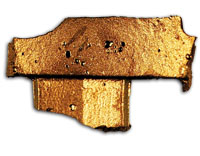
\includegraphics[width=\textwidth]{Chapter0/Graphics/porosity1.jpg}
	\caption{Gas porosity in casting}
    \label{fig:porosity1}
  \end{subfigure}
   %------------
   \hspace{1cm}
   \begin{subfigure}[t]{0.25\textwidth}
    \centering
	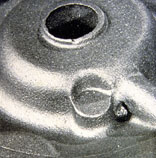
\includegraphics[width=\textwidth]{Chapter0/Graphics/porosity2.jpg}
	\caption{Shrinkage porosity}
    \label{fig:porosity2}
  \end{subfigure}
  %------------------------------
  \vskip\baselineskip
  %------------------------------
  \begin{subfigure}[t]{0.3\textwidth}
    \centering
	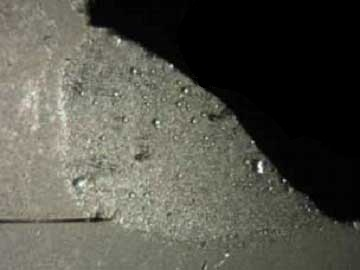
\includegraphics[width=\textwidth]{Chapter0/Graphics/porosity3.jpg}
	\caption{Gas porosity in aluminium welding}
    \label{fig:porosity3}
  \end{subfigure}
   %------------
  \hspace{1cm}
   \begin{subfigure}[t]{0.25\textwidth}
    \centering
	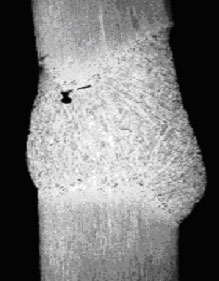
\includegraphics[width=\textwidth]{Chapter0/Graphics/porosity4.jpg}
	\caption{Xray of volume void inside welded duplex steel}
    \label{fig:porosity4}
  \end{subfigure}
   %------------
\caption{Examples of porosity in casting and welding} 
\label{fig:porosity}
\end{figure}
%-------------------------------------------------------------------------------------------------------------------------------------------------
\subsection*{Freckles or segregated channels} 
The origin of this defect is a combined effet of microsegregation and buoyancy forces. 
Upon solidification, solid forms while rejecting some solute in the liquid due to partitioning (steels have a partition coefficient less than unity).
When the segregated solute is the lighter species, an increasing concentration in the liquid phase produces a solutal driving force inside the mushy zone, generating unstable convection currents, with "plume" shapes as often reported in the literature \citep{sarazin_studies_1992, schneider_modeling_1997, shevchenko_chimney_2013}. When temperature gradient is an additional force of convection, the latter is termed "thermosolutal".
%-------------------------------------------------------------------------------------------------------------------------------------------------
\section{Macrosegregation}
Macrosegreation generally stems from a solubility difference between a liquid phase and one or more solid phases, along with
a relative velocity between these phases. While the former is responsible for local solute enrichment or depletion, the latter
will create the composition heterogeneity on a scale much larger than just a few dendrites.
% http://dictionary.cambridge.org/grammar/british-grammar/little-a-little-few-a-few
This is why macrosegregation could be observed on the scale of a casting, up to several meters in length. 
%--------------------------------------------------------
\subsection{Causes}
Four main factors can (simultaneously) cause fluid flow leading to macrosegregation:
\subsubsection*{Liquid dynamics}
During solidification, thermal and solutal gradients result in density gradients in the liquid phase: 
\begin{subequations}
\begin{align}
\label{eq:rholiq}
& \rhol = \rhoref ( 1 - \betaT (T - \Tref) - \sum_{i} \betawil (\wil - \wilref) )  \\ 
\label{eq:gradrholiq}
& \nabvec\rhol = -\rhoref (  \betaT \nabvec T + \sum_{i} \betawil \nabvec\wil  )
\end{align}
\end{subequations}
In \cref{eq:rholiq}, density is assumed to vary linearly with temperature and phase composition for each chemical species (index $i$).
The slopes defining such variations are respectively the thermal expansion coefficient $\betaT$ and solutal expansion coefficient $\betawil$, given by \citep{kohler_peritectic_2008}:
\begin{subequations}
\begin{align}
\label{eq:betaT}
& \betaT =  -\frac{1}{\rhoref} \brac{\frac{\partial\rhol}{\partial T}}  \\ 
\label{eq:betawil}
& \betawil = -\frac{1}{\rhoref} \brac{\frac{\partial \rhol}{\partial \wil}}  
\end{align}
\end{subequations}
The linear fit assumes also that the density takes a reference value, $\rhoref$, when temperature and liquid composition reach reference values, respectively
$\Tref$ and $\wilref$. However, in some situations, a suitable thermodynamic database providing accurate density values is far better than a linear fit, especially in the current context of macrosegregation. 
Such possibility will be discussed later in the manuscript (cf. SECTION TODO ) %TODO 
In the presence of gravity, the density gradient in \cref{eq:gradrholiq}, causes thermosolutal convection in the liquid bulk and a subsequent macrosegregation.
 
\subsubsection*{Solidification shrinkage}
Solid alloys have a greater density than the liquid phase ($\rhos > \rhol$), thus occupy less volume. Upon solidification, the liquid moves towards the solidification front to compensate for the volume difference caused by the phase change, as well as the thermal contraction. When macrosegregation is triggered by solidification shrinkage,
we speak of \emph{inverse segregation} Theoretically, if solute mass is conserved, a decreasing volume results in a positive segregation. Shrinkage deforms the outer
surface of a solidifying alloy, causing positive macrosegregation. While one would naturally expect negative macrosegregation in areas where solidification begins and positive inside the alloy, shrinkage promotes the opposit phenomenon, hence the term \emph{inverse segregation}.
In contrast to liquid convection, shrinkage flow may cause macrosegregation even without gravity.

\subsubsection*{Movement of equiaxed grains}
Equiaxed grains can grow in the liquid bulk where thermal gradients are weak, or in the presence of inoculants. Consequently, 
they are transported by the flow (floating or sedimenting, depending on their density \citep{beckermann_modelling_2002}) which leads to negative macrosegregation in their final position.

\subsubsection{Solid deformation} 
Stresses of thermal and mechanical nature are always found in casting processes (e.g. bulging between rolls in continuous casting). 
Deformation of the semi-solid in the mushy zone causes a relative solid-liquid flow in the inward (tensile stresses) or outward (compression stresses) direction, causing macrosegregation.
%--------------------------------------------------------------------------------------------------------------------------------------------------
\subsection{Types}
\subsubsection*{In continuous casting}
The semi-solid billet is carried through a series of rolls that exert a radial force to straighten it and get it to its horizontal position.
As the mushy part of a slab enters through these rolls, interdendritic liquid is expelled backwards, i.e. regions with lower solid fraction.
Since the the boundaries solidify earlier than the centre, the enriched liquid accumulates halfway in thickness, forming a centreline macrosegregation
as shown in \cref{fig:macroseg_centreline}. Other types of segregates (channels, A-segregates ...) can also be found but remain more specific to ingot casting. 
\begin{figureth}
% macrosegregation_centreline_zoom: http://goo.gl/iKPNfz
% textwidth 
{1.0}
%path 
{Chapter0/Graphics/macrosegregation_centreline_zoom.pdf}
% caption
{Centreline segregation in a steel slab \citep{beckermann_modelling_2002}}
% label
\label{fig:macroseg_centreline}
\end{figureth}
%--------------------------------------------------------
\subsubsection*{In ingot casting}
A variety of segregation patterns can be encountered in heavy ingots: 
\begin{itemize}
\itemsep0em 
\item the lower part is characterized by a negative segregation cone promoted by the sedimentation of 
	  equiaxed crystals,
\item positive segregation channels, known as A-segregates, form along the columnar dendritic zones, close to the vertical contact with the mould,
\item positive V-segregates can be identified in the centre of the ingot,
\item a positive macrosegregation in the upper zone where the last liquid solidifies, the so-called "hot-top", caused by solidification shrinkage (inverse segregation)
	  and thermosolutal buoyancy forces. 
\end{itemize}
\citet{combeau_prediction_2009} state that A-segregates and V-segregates formation is mainly attributed to local flow phenomena.
As such, their scale is finer than macrosegregation, hence called "mesosegregates".
%-----------------------
\begin{figureth}
{0.6}
{Chapter0/Graphics/macrosegregation_ingot.png}
{Sulphur print (left) of a 65-ton steel ingot showing various patterns (right) of macrosegregation \citep{flemings_solidification_1974, lesoult_macrosegregation_2005}}
\label{macrosegregation_ingot}
\end{figureth}
%--------------------------------------------------------
\subsubsection*{In investment casting}
This process is widely used to cast single-crystal (SC) alloys for turbines and other applications that require excellent mechanical behavior \citep{giamei_nature_1970}.
During directional solidification, thermosolutal forces thrust segregated species outside of the mushy zone into the liquid bulk.
The segregation scale ranges from a few dendrites to a few hundreds of them, hence forming "long and narrow trails" (\cref{fig:freckle1}) as described by \citet{felicelli_simulation_1991}. Freckles are frequently formed by small equiaxed grains (\cref{fig:freckle2}), probably caused by a uniform temperature gradient 
that settles as the channels become richer in solute. They can be observed on the ingot's surface, as well as in the volume.
\begin{figure}[htbp]
%freckle1: http://user.engineering.uiowa.edu/~becker/solcast.html
%freckle2: beckermann 2002 or Giamei ?
%freckle3: Giamei 
\centering
   %------------
  \begin{subfigure}[t]{0.25\textwidth}
    \centering
	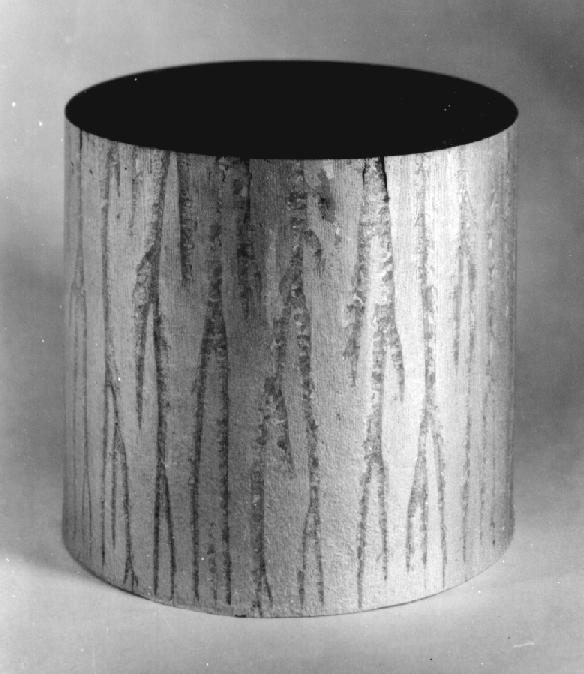
\includegraphics[height=5cm]{Chapter0/Graphics/freckle1.png}
	\caption{WRITE}
    \label{fig:freckle1}
  \end{subfigure}
   %------------
   \qquad %\hspace{2cm}
   \begin{subfigure}[t]{0.25\textwidth}
    \centering
	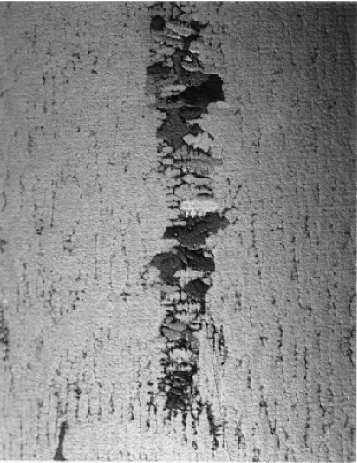
\includegraphics[height=5cm]{Chapter0/Graphics/freckle2.png}
	\caption{WRITE}
    \label{fig:freckle2}
  \end{subfigure}
   %------------
\caption{Freckles in directional casting of nickel-base superalloys} 
\label{fig:freckle}
\end{figure}
%--------------------------------------------------------
\section{Industrial Worries}
\textbf{Steel production} has continuously increased over the years to meet the industrial needs. \Cref{fig:steel_production} shows this increase between 1980 and 2013 with a 
clear dominance of the Chinese production. Quality constraints have also increased where specific grades of steel are needed in critical applications such as mega-structures
in construction and  heavy machinery. Therefore, alloys with defects are considered vulnerable and should be avoided as much as possible during the casting process. As such, steelmakers have been investing
in research, with the aim of understanding better the phenomena leading to casting problems, and improve the processes when possible.
\begin{figure}[htbp]
\centering
\begin{tikzpicture}
 \pgfkeys{%
    /pgf/number format/set thousands separator = {}}
\begin{axis}
[
	table/col sep=comma,
	smooth, %ybar
	stack plots=y,
	area style,
	enlarge x limits=false,
	legend pos=north west,
	scaled ticks=true,
	xlabel=Year,
	ylabel=Production (tons),
	xticklabel style={/pgf/number format/fixed},
	xtick={1980,1990,2000,2010},
	%x tick label style={rotate=45,anchor=east},
	%width=0.5\textwidth
]
\addplot table [x=Year, y expr=\thisrow{EU}*1000] {Chapter0/Data/steel_production.csv} \closedcycle ;
%\addlegendentry{EU (27)}
\addplot table [x=Year, y expr=\thisrow{China}*1000] {Chapter0/Data/steel_production.csv}\closedcycle;
%\addlegendentry{China}
\addplot table [x=Year, y expr=\thisrow{World}*1000] {Chapter0/Data/steel_production.csv}\closedcycle;
%\addlegendentry{World}
\legend{EU (27), China, World}
\end{axis}
%\addplot table [x expr=\coordindex, y=EU] {Chapter0/Data/steel_production.csv};
\end{tikzpicture}
\caption{Evolution curves of crude steel worldwide production from 1980 to 2013}
\label{fig:steel_production}
\end{figure}

\textbf{Simulation software} dedicated to alloy casting is one of the main research investments undertaken by steelmakers. These tools coming from academic research
are actively used to optimize the process. However, few are the tools that take into account the casting environment. For instance, the continuous casting process, in
\cref{fig:cc_process}, is a chain process where the last steps involve rolls, water sprays and other components. A dedicated software is one that can provide the
geometric requirements with suitable meshing capabilities, as well as respond to metallurgical and mechanical requirements, mainly:
\begin{itemize}
\itemsep0em
\item handling moulds and their interaction with the alloy (thermal resistances ...)
\item handling alloy filling and predicting velocity in the liquid and mushy zone
\item handling thermomechanical stresses in the solid
\item handling multicomponent alloys and predicting macrosegregation
\item handling finite solute diffusion in solid phases
\item handling real alloy properties (not just constant thermophysical/thermomechanical properties)
\end{itemize}
%-------------------------------------------------------------------------------------------------------------------------------------------------
\section{Objectives and outline}
%--------------------------------------------------------
\subsection*{\ccemlcc project}
Since its foundation in 1975, the European Space Agency (ESA) has been actively committed in the research field.
Their areas of activity cover not only exclusive space applications, but also fundamental science related to 
physics and other disciplines. This thesis takes part of the ESA project entitled \ccemlcc, abbreviating
"\textbf{C}hill \textbf{C}ooling for the \textbf{E}lectro-\textbf{M}agnetic \textbf{L}evitator in relation with 
\textbf{C}ontinuous \textbf{C}asting of steel".
The three-year contract from 2011 to 2014 denoted \ccemlcc II, was preceded by an initial project phase, \ccemlcc I,
from 2007 to 2010. The main focus is studying containerless solidification of steel under microgravity conditions. 
A chill plate is used to extract heat from the alloy, simulating the contact effect with a mould in continuous casting
or ingot casting.
CEMEF contributed to the work by proposing numerical models and simulation tools in view of predicting the chill cooling of steel droplets. 
A first model was developed by \citet{rivaux_simulation_2011} whereas the present discusses a new model. 
The experimental work considered various facilities and environments to set a droplet of molten alloy in levitation: electromagnetic levitation (EML) 
for ground-based experiments, microgravity in parabolic flight or sounding rockets and last, microgravity condition on-board the International Space Station (ISS)

\begin{figureth}
% textwidth 
{0.5}
%path 
{Chapter0/Graphics/eml1.jpg}
% caption
{Electromagnetic levitation}
% label
\label{fig:eml}
\end{figureth}

\comment{in what ways does this project tries to alleviate the aforementionned problems ?
The two phases of CCEMLCC, together with the newly coming \ccemlcc III, aim to shape our understanding
of solidification with thermo-mechanical stresses under microgravity conditions.}
%-------------------------------------------------------------------------------------------------------------------------------------------------
Numerical tools: Cimlib relying on PETSc, parallelized with MPICH2, paraview and python as tools for postprocess and analysis. \\
The previously mentionned simulation requirements are not met in a single casting software package. Nevertheless, \thercast is a promising tool that already 
handles a part of the above points. The current thesis developments are done using C++ language as a part of the
in-house code, known as \cimlib \citep{digonnet_cimlib:_2007, mesri_advanced_2009}. 
This fully parallel library is the main academic research support for \thercast.\\ \\ 

Aims of this research (+novelty of the work)\\ 
\begin{itemize}
\item solidification model with level set air-metal +darcy in the metal
\item Tracking of the interface induced by shrinkage
\end{itemize}
Each chapter content
%--------------------------------------------------------
\subsection*{Biblio test}
\citet{carozzani_direct_2013} is textual \\
\citep{carozzani_direct_2013} is parenthetical \\
%--------------------------------------------------------
\subsection*{Cross reference test}
ref gives \ref{eq:betaT} \\
cref gives \cref{eq:betaT} \\
Cref gives \Cref{eq:betaT} \\
autoref gives \autoref{eq:betaT} \\


ref gives \ref{fig:porosity1} \\
cref gives \cref{fig:porosity1} \\
Cref gives \Cref{fig:porosity1} \\
autoref gives \autoref{fig:porosity1} \\


%\section*{Trying \emph{SIUNITX}}
%Here i wana test the SI units package via the commands \num{.3e45} and the unit \si{\kilo\metre}
%then i wanted to see if we combine both via \SI{.3e45}{\kilo\metre} then finally my personal command
%\SI{231e-4}{\uacceleration} \\
%\SI{231e-4}{\ucomposition} C \\
%\SI{231e-4}{\uvelocity} \\
%\SI{231e-4}{\uconductivity} \\
%\SI{231e-4}{\umasscapacity} \\
%\SI{231e-4}{\uvolumecapacity} \\
%Will it work \num{.3e45}   ,  \num{3.45d-4}   , \numlist{10;30;50;70} ,  \numrange{10}{30} % Introduction

\chapter{Modelling Review}
\minitoc
\newpage

In this chapter the following points are discussed
\begin{itemize}
\item what does a typical solidifications problem consist of ? heat - fluid - solid 
- chemical species
\item what are the modeling scales of these physics ? direct (micro: phase field / macro: CA) 
and indirect (micro Nancy models / macro: current FE model)
\comment{Maybe worth showing the 2x2 table that CAG showed at the ICASP conference ?}
\item Overview of these models ??
\item Presence of AIR requires a new problem definition : Lagrangian or Eulerian framework
\end{itemize}


\section{FE model}
A section presenting the main FE equations that will be solved in the metal being a single domain.
\begin{itemize}
\item Energy (chapter 1)
\item
\end{itemize}

\comment{talking about Eulerian approach Air Metal will be presented in the next chapters}

\section{Biblio test}
\cite{carozzani_direct_2013} are going to appear in the paper  % Modelling Review
\chapter{Energy balance with thermodynamic tabulations}
%\chaptermark{Energy Balance with thermodynamic tabulations}
\begin{nolinkcolors} 
\minitoc
\end{nolinkcolors}
\newpage
%
%
%=====================================
\section{State of the art}
%=====================================
\comment{ Use of enthalpy resolution in the majority of works \\
 motivation and advantages of TvsH without talking about resolution time\\
 use article's introduction to fill this section (or improvise new things)}
%
When speaking about macrosegregation, one needs to know that the problem involves phase change.
For that, a minimum of four conservation equations are necessary:
conservation  of  mass, momentum,  chemical  species and  energy. The  phase  change
literature  contains a  wealth of numerical methods to solve energy conservation
in solidifying alloys. A comprehensive overview of these methods is given by \citet{swaminathan._enthalpy_1993}.
The corresponding equation associates the total average enthalpy to the
temperature  via  intrinsic  alloy  properties, such  as the heat  capacity of  the
phases and the latent  heat associated with the phase transformations. However, in the course
of solidification and while macrosegregation is taking place, these  properties may change because the average
composition may  vary  significantly: the  transformation paths are thus modified, as well as
the phases' composition and heat capacity. Similarly, the latent heat of phase  transformations
is  not a mere constant that could be distributed as a function of the phase fractions
assuming only temperature-dependent phases' properties, as often found in the literature \citep{bellet_call_2009}.
It is thus impossible to establish a priori the dependence of the enthalpy with respect
to temperature when macrosegregation takes place, even in the case of full thermodynamic equilibrium
between phases. In this chapter, we discuss a suitable numerical scheme based on an enthalpy method,
already used in the literature  to  alleviate this macrosegregation-related problem \citep{swaminathan._enthalpy_1993,
carozzani_direct_2013}. Later on, we introduce a modified formulation, using the effective heat capacity method that 
increases the original scheme's efficiency. 

The current method is thus an enthalpy method that makes use of a temperature-based solver. 
Moreover, it uses tabulated thermodynamic quantities (solidification paths, phases' enthalpy  and composition) 
in a range of average compositions and temperatures as found in the literature 
\citep{dore_modelling_2000,thuinet_prediction_2004,du_modeling_2007}, 
with the aim of evaluating the total average enthalpy as well as the effective heat capacity. 
The novelty of the modified method resides in the use of thermodynamic tabulations without losing 
the advantages of the previous method, thus yielding faster computation times while maintaining a 
good accuracy.
%
%
%=====================================
\section{Thermodynamic considerations}
%=====================================
%
%-----------------------------
\subsection{Volume averaging} 
%-----------------------------
\comment{the following paragraph will be deleted once the volume averaging has been introduced in chapter 1}
\red{A volume averaging technique was suggested to deal with the presence of multiple 
phases \citep{ni_volume-averaged_1991}. It locally considers a Representative Volume Element 
(RVE) that contains a single or several phases (these are not necessarily in thermodynamic equilibrium) 
at a mesoscopic scale. We represent, for each unknown $\psi$, an intrinsic volume average, $\avg{\psi}^{\phi}$ (also denoted $\avg{\psi^{\phi}}^{\phi}$ in the 
literature), corresponding to a phase $\phi$. 
The volume average $\avg{\psi}$ for this unknown in the RVE, hence averaged over all the present phases writes:}
%%-------------
\begin{align}
\label{eq:volume_average_psi}
& \avg{\psi} = \sum_\phi \gphi \avg{\psi}^{\phi}
\end{align}
%%-------------
where $g^\phi$ denotes the volume fraction of phase $\phi$ in the RVE. 
It should be emphasized that the averaging technique applies to virtually all thermodynamic variables (enthalpy, density $\dots$). 
Among these variables, the temperature is also considered to be uniform in the RVE. 
Applying the volume averaging technique to the energy 
conservation principle along with interfacial balances between the phases, results in the following averaged equation \citep{rappaz_numerical_2003}:
%%-------------
\begin{align}
\label{eq:averaged_energy_eqn}
& \frac{\d \rh}{\d t} + \nabvec \cdot \rhv = \nabvec \cdot \brac{\avg{\kappa} \nabvec T} + \avg{\dot{Q}_V}
\end{align}
%%-------------
where $\rho$ stands for the density, $h$ the mass enthalpy, $\vec{v}$ the velocity field, $\kappa$ the thermal conductivity, $T$ the temperature 
and $\dot{Q}_V$ a possible volume heat source. 
\Cref{eq:averaged_energy_eqn} is the standard averaged form of the energy conservation equation used in non-stationary phase 
change problems. 
\comment{ I could elaborate more in this paragraph by showing the possible equations for the explicit formulation and maybe a figure to show the AlSi7
computation that i did with a v small time step }
 
Once the variational form has been discretized in space and time, two possible resolution schemes emerge: the first is an 
explicit forward Euler scheme which gives rise to a linear equation where the temperature is known at time $t$, $T^t$. This requires very small 
time steps in the current context, which limits the solver’s usability at the scale of industrial applications. The second scheme is the 
backward Euler or full implicit discretization where terms are function of $T^{t+\Delta t}$. It leads to a nonlinear equation with 2 interdependent 
unknowns, $\rh^{t+\Delta t}$ and  $T^{t+\Delta t}$. It is clear that the nature of the temperature-enthalpy relationship plays a central 
role when formulating the resolution strategy of this nonlinear equation. Generally, it is admitted that, depending on the resolution strategy, 
it is necessary to express enthalpy as a function of temperature or vice-versa, together with associated partial derivatives, 
$\frac{d \rh}{dT}$ or $\frac{dT }{d \rh}$.

\subsection{The temperature-enthalpy relationship} 
In solidification problems, additional variables are involved in \cref{eq:volume_average_psi} and \cref{eq:averaged_energy_eqn}, 
like the transformation path that defines the history of the phase fractions, as well as the average chemical composition $\wi$, 
i being the index of the chemical species (only the solutes are considered). The temperature-enthalpy relation averaged over the 
phases in a given RVE writes:
%%-------------
\begin{align}
\label{eq:volume_average_enthalpy}
& \rh = \sum_\phi \gphi_{\brac{T, \wi \dots}} \rphi_{\brac{T, \wi^{\phi} \dots}} \hphi_{\brac{T, \wi^{\phi} \dots}}
\end{align}
%%-------------
Note that the volume average enthalpy is approximated by the product $\avg{\rho h}^{\phi}=\avg{\rho}^{\phi}\avg{h}^{\phi}$ in the current work. As stated 
in the introduction, it becomes clear from \cref{eq:volume_average_enthalpy} that phase properties, i.e. average phase density, , \rphi and enthalpy, \hphi, 
are temperature and composition dependent. This equation is the key to convert the average volume enthalpy to temperature (through a procedure named \HtoT) 
or vice-versa (\TtoH). The values of the different phase fractions $\gphi$ (solidification path) and phase enthalpies $\rh^{\phi}$ are thus needed 
to close the relation.

\subsection{Tabulation of properties}
The complexity of performing a thermodynamic conversion is directly linked 
to the simplicity of determining the alloy properties, namely the phase fractions 
and phase enthalpies. In the case of binary alloys and with several assumptions 
with respect to the system (e.g., linear monovariant temperature composition 
relationships, constant heat capacity of phases and constant latent heat of transformations, 
equilibrium approximations between phases) analytical calculations are often used to determine 
the properties. Nevertheless, analytical relations are more complex or even impossible to derive 
in the case of multicomponent alloys ($i>1$). To overcome this problem, one can resort to 
thermodynamic databases and phase equilibrium calculations to tabulate the transformation paths 
and the phase enthalpies for a given range of temperatures and average compositions. It is a handy 
solution for two main reasons: first, the conversion is merely a binary search in a table; secondly, 
it is a simple solution for coupling with macrosegregation. In this way, phase fractions $\gphi$ are 
tabulated as functions of temperature and average composition, while for each phase $\phi$ the mass 
enthalpy, $\hphi$, and the density, $\rphi$, are tabulated as functions of temperature and phase 
intrinsic average compositions $\wiphi$, as well as other possible parameters. \Cref{Table:t2h_data} summarizes the 
steps in order to perform a temperature-to-enthalpy (\TtoH) conversion using the predefined tabulation 
approach. In step 1, the transformation path is acquired for each average composition and temperature 
to determine the list of phases, their volume fractions $\gphi$ and their intrinsic compositions $\wi^{\phi}$. 
In step 2, the phase enthalpy $\hphi$  and density $\rphi$ are determined by searching for the temperature and 
the already known phase composition $\wi^{\phi}$. In step 3, the average volume enthalpy is computed from the 
volume fraction, density and mass enthalpy of phases using \cref{eq:volume_average_enthalpy}.
%
%---------------------------
% this table did not work when using custom tabulate env. because of the call to \cref ?
\begin{table}[htbp]
\centering
\caption{Tabulation processing for a \TtoH procedure}
\label{Table:t2h_data}
{\tabulinesep=1.0mm
\begin{tabu}{|c|c|c|c|}
\tabucline[1pt]{-}
\textbf{Step Number} 	& 	\textbf{1}	& \textbf{2}	& 	\textbf{3} 				\\\tabucline[1pt]{-}
\textbf{Inputs} 		&  ${T,\wi}$	& ${T,\wiphi}$	&	${\gphi, \rphi \hphi}$ \\
\textbf{Outputs} 		&  ${\gphi,\wiphi}$	& ${\rphi,\hphi}$	&	${\avg{\rho h}}$ (\cref{eq:volume_average_enthalpy})
				\\\tabucline[1pt]{-}
\end{tabu}}
\end{table}
%---------------------------
%
The methodology to build the tabulations is straightforward. It is based on two main scans. On the one hand, intervals for the variation of the 
average composition $\wi$ are chosen from the known alloy composition. These variations have to cover the extreme values adopted during the 
simulation, which are not known a priori. An interval is also selected for the variation of temperature. The latter is easier to determine as it
usually starts from the initial melt temperature and goes down to the room temperature in a standard casting simulation. For these intervals, a 
systematic scan is made with chosen steps in each composition and T, during which a thermodynamic equilibrium is computed. The outputs are the 
number of phases encountered, together with their fraction and intrinsic composition. The minimum and maximum intrinsic composition for each phase 
could then be determined. On the other hand, for each phase, a scan of the intrinsic composition and temperature is made to compute the intrinsic 
properties. The same temperature interval and step as defined earlier are used.

\comment{ below paragraph should be re written and maybe stress LESS on the speed effect}
\comment{ I should change the superscript $k$ which may be confused with partition coefficient }
Regarding the enthalpy-to-temperature conversion (\HtoT), a backward iterative \TtoH search is performed. 
For a known composition $\wi$, denoting $k$ the iteration index to convert the enthalpy 
$\avg{\rho h}_{\text{input}}$, we start with an initial guess for temperature $\Tkinit$ then convert it to an 
enthalpy  $\Hkinit$ with the \TtoH conversion. Using an appropriate nonlinear algorithm (Brent is the most versatile 
in our case), we aim at minimizing the following residual: $\text{Residu}_{\rh} = \abval{\rh_{\text{input}} - \Hk }$. 
Once the algorithm has converged, the temperature $\Tk$ is the result of the \HtoT conversion. It is 
inferred that the first conversion (\TtoH) is a direct one whereas the latter (\HtoT) is indirect and requires 
a series of iterative steps; each step being a single \TtoH resolution. In other words, a \HtoT conversion is a 
backward search for a temperature, hence it’s slower. This conversion’s speed lag is exacerbated when tabulations 
increase in size (e.g. large number of temperature and composition steps) and complexity (e.g., multicomponent 
industrial alloys used in casting), since the search gets more complicated with the increasing number of input 
columns (one column for each alloying element).
%
%
%==================
\section{Numerical method}
%==================
%
The finite element method is used to solve the energy conservation as expressed by \cref{eq:averaged_energy_eqn}. 
A test function $\test$ belonging to the Hilbertian Sobolev space $\hilbert(\Omega)$ of continuous integrable test functions 
is used to formulate the integral variational form of \cref{eq:averaged_energy_eqn} \citep{suli_lecture_2000}. 
A Fourier boundary condition is considered on the domain boundary $\partial \Omega$. The domain $\Omega$
is discretised using first-order linear simplexes defined by their number of local nodes (denoted “NbLoc”): triangles 
in 2D with NbLoc=3 and tetrahedra in 3D with  NbLoc=4. The outcome is a residual that we aim to minimize so that the 
conservation principle is satisfied. Therefore, the weak form writes:
%----------------------
\begin{multline}
\label{eq:weak_energy}
\forall \test \in M=\curly{u \in \hilbert(\Ohm)} \\
\integral{\Ohm}{\test \tempup{\rhoh}}{V} 
 + \integral{\Ohm}{\test \vit \cdot \nabvec \brac{\rhol \hl}}{V}
 - \integral{\Ohm}{\test \diff{\avg{\kappa}}{T} }{V}
 - \integral{\Ohm}{\test \source }{V}
 = 0
\end{multline}
%------------
where we assumed a static solid phase and an incompressible liquid phase, which allowed recasting the second term of 
\cref{eq:averaged_energy_eqn} into $\vit \cdot \nabvec \brac{\rhol \hl}$. 
The steps for discretizing in time and space the previous equation are well detailed in  some book references like \citet{rappaz_numerical_2003,dantzig_solidification_2009}. As for enthalpy and temperature, they are spatially discretized in each simplex 
using interpolations functions $\interp$, thus defining the nodal values $H_j$ and $T_j$, respectively: 
%----------------------
\begin{align}
\label{eq:discretise_H}
\rhoh 	&= \sum_{j=1}^{\text{NbLoc}}  \interp_j   \Hj \\ 
\label{eq:discretise_T}
T		&= \sum_{j=1}^{\text{NbLoc}}  \interp_j   \Tj
\end{align}
%------------
Note that $H_j$ is a volumetric enthalpy. The Galerkin formulation gives the following expression for the residual contribution at a mesh node $i$ for time step $t$ in a local element $\element$:
%----------------------
\begin{align}
\begin{split}
\label{eq:discretise_residual_local}
& \brac{R_i^E}^t = \Mij^E \brac{\Hjt - \Hjtminus} + \Aij^E \Tjt + \brac{\Kija^E + \Kijb^E}-\Fi^E - \Si^E=0 \\
& i,j:1 \rightarrow \text{NbLoc}
\end{split}
\end{align}
%------------
where the numerical contributions can be detailed as follows:
%----------------------
\begin{align}
& \textit{transient term:} \quad  \Mij^E = \integral{\OhmE}{\frac{1}{\dt} \interp_i \interp_j }{V} \\ 
& \textit{advection term:} \quad  \Aij^E = \integral{\OhmE}{\rhol \cpl \interp_i \vit \cdot \nabvec \interp_j}{V} \\ 
& \textit{diffusion term:} \quad  \Kija^E = \integral{\OhmE}{\avg{\kappa} \nabvec \interp_i\nabvec \interp_j}{V} \\ 
& \textit{boundary condition term 1:}	\quad  \Kijb^E = \integral{\dOhmE}{\hext \interp_i \interp_j}{S} \\ 
& \textit{boundary condition term 2:}	\quad	\Fi^E = \integral{\dOhmE}{\hext \Text \interp_i}{S} \\
& \textit{source term:} \quad  \Si^E = \integral{\OhmE}{\interp_i \source}{V}
\end{align}
%------------
%
The surface integrals $\Kijb^E$ and $\Fi^E$ are related to a Fourier-type boundary condition, 
with $\hext$ as a coefficient of heat exchange and $\Text$ as the external temperature far from the 
boundary. The energy conservation principle is satisfied when the sum of the residual contributions 
coming from all the mesh elements is zero. In other words, the following global residual defined by 
the assembly of these contributions, should be minimized: 
%----------------------
\begin{align}
\begin{split}
\label{eq:discretise_residual_global}
& \brac{R_i}^t = \Mij \brac{\Hjt - \Hjtminus} + \Aij \Tjt + \brac{\Kija + \Kijb}\Tjt -\Fi - \Si=0 \\
& i,j:1 \rightarrow \text{NbGlob}
\end{split}
\end{align}
%------------
where the global tensors $\Mij$, $\Aij$, $\Kija$ , $\Kijb$ , $\Fi$ and $\Si$ contain respectively, after an assembly step, 
the contributions of the local matrices $\Mij^E$, $\Aij^E$, $\Kija^E$ , $\Kijb^E$ , $\Fi^E$ and $\Si^E$ from each discretised 
element in the domain $\Ohm$. Accordingly, the indices $i$ and $j$ refer to global node numbers, where the total number of nodes is 
denoted by "NbGlob". It is clear that the global residual inherits the dependence between enthalpy and temperature. 
This is shown in \cref{eq:discretise_residual_global} where the average volume enthalpy is a function of the temperature. It infers that this residual 
is a non-linear function; therefore minimizing it requires an iterative non-linear algorithm. Our choice settles on the 
Newton-Raphson method, known for its quadratic convergence speed. A solidification problem can induce severe non-linearities 
from the release of the latent heat (which itself is temperature-composition dependent) and the variations of the thermophysical 
properties of the alloy with respect to temperature and average composition. This algorithm could thus treat such variations. 
Considering the link between enthalpy and temperature, \cref{eq:discretise_residual_global} may be solved either for enthalpy 
or for temperature as a nodal unknown; hence both formulations are presented hereafter.
%
%
%---------------
\subsection{Enthalpy-based approach }
%---------------
The residual is re-written using a Taylor series expansion to the first order for a nonlinear iteration $\iter$ :
%-----------------
\begin{align}
\label{eq:Hsolver_residual}
& \brac{R_i}^\iterplus = \brac{R_i}^\iter + \brac{\dRdH}^{\iter}_{ij} \Delta \Hj^\iter + \order\brac{\Hj^2}
\end{align}
%------------
Neglecting the second order terms, the suggested correction at each iteration in view of cancelling 
the residual and giving the new value $\Hj^\iter$, is given by the linear system in \cref{eq:Hsolver_residual_linear}
relative to what we call a \emph{Hsolver}:
%-----------------
\begin{align}
\label{eq:Hsolver_residual_linear}
& \brac{\dRdH}^{\iter}_{ij} \brac{\Hj^\iterplus - \Hj^\iter} = -R_i^\iter
\end{align}
%------------
where $\dRdH$ is a global tangent matrix yielding the variations of the residual with respect to the enthalpy 
in the last iteration, $\Hj^\iter$. If \cref{eq:discretise_residual_local} is considered, then the contribution of an element $\OhmE$ writes:
%-----------------
\begin{align}
\label{eq:dRdH}
& \brac{\dRdH}^{\iter E}_{ij} 
= \Mij^E 
+ \underbrace{\Aij^E \brac{\dTdH}^{\iter}_{j}}_{\nosum}
+ \underbrace{\brac{\Kija^E + \Kijb^E} \brac{\dTdH}^{\iter}_{j}}_{\nosum}
\end{align}
%------------
\Cref{eq:dRdH} is the core of the enthalpy-based solver. The resolution of \cref{eq:Hsolver_residual_linear} 
then yields a new estimate of the vector of nodal enthalpies $H^\iterplus$, which are the only unknowns to be solved for. 
Once determined at iteration $\iter$, convergence tests are performed (refer to section %TODO ).
%
%
%---------------
\subsection{Temperature-based approach }
%---------------
Similarly to the Hsolver, the local residual is recast for a nonlinear iteration $\iter$, 
leading this time to an iterative temperature correction:
%-----------------
\begin{align}
\label{eq:Tsolver_residual_linear}
& \brac{\dRdT}^\iter_{ij} \brac{\Tj^\iterplus - \Tj^\iter} = -R_i^\iter
\end{align}
%------------
where $\dRdT$ is a global tangent matrix yielding the variations of the residual with respect to temperature $\Tj^\iter$ at the previous iteration. 
This solver will be referred to as \emph{Tsolver}.
The contribution of an element $\OhmE$ to this tangent matrix is evaluated as:
%-----------------
\begin{align}
\label{eq:dRdT}
& \crochet{\dRdTijk}^E
= \Mij^E 
+ \underbrace{\Aij^E \brac{\dHdT}^{\iter}_{j}}_{\nosum}
+ \underbrace{\brac{\Kija^E + \Kijb^E} \brac{\dHdT}^{\iter}_{j}}_{\nosum}
\end{align}
%------------
In contrast to the previous solver, \cref{eq:dRdT} is the core of the temperature-based solver. The resolution of \cref{eq:Tsolver_residual_linear} 
then yields a new estimate of the vector of nodal temperatures $T^\iterplus$, which are the only unknowns to be solved for. 
Once updated for iteration $\iter$, convergence tests are performed (refer to section %TODO ).
%
%
%-------------------
\subsection{Convergence}
%
The previous two sections described the iterative resolution of the same discretised energy 
conservation by both Tsolver and Hsolver. However, in \cref{eq:dRdH,eq:dRdT}, an important 
term emerges from the tangent matrix evaluation describing the variations between temperature 
and enthalpy: $\dHdT$ (or $\dTdH$). This term invokes the previously mentioned temperature-enthalpy 
tabulations which depend on the alloy composition. Consequently,  $\dHdT$ (or $\dTdH$)
has a great influence on the convergence of the Tsolver (respectively the Hsolver). 
When \cref{eq:Hsolver_residual_linear} or \cref{eq:Tsolver_residual_linear} is solved at iteration $\iter$, this term is written using a finite difference:
%-----------------
\begin{align}
\label{eq:finite_difference_Tsolver}
& \textbf{Tsolver} \qquad \brac{\dHdT}^{\iterplus}_{j} = \frac{\rhoh_j^\iterplus - \rhoh_j^\iter}{T_j^\iterplus - T_j^\iter} \\
\label{eq:finite_difference_Hsolver}
& \textbf{Hsolver} \qquad \brac{\dTdH}^{\iterplus}_{j} = \frac{T_j^\iterplus - T_j^\iter}{\rhoh_j^\iterplus - \rhoh_j^\iter}
\end{align}
%------------
For the Tsolver, the enthalpy $\rhoh_j^\iter$ is needed to evaluate \cref{eq:finite_difference_Tsolver}. 
In contrast, the Hsolver requires the value of $T_j^\iter$ to evaluate the corresponding \cref{eq:finite_difference_Hsolver}.
In both cases, the unknown is determined by the temperature-enthalpy relation. The indices next to the mentioned unknowns
indicate that this relation is used for each iteration $\iter$ at each mesh node $j$, hence affecting the global resolution time 
between the two solvers. The Hsolver needs a \HtoT to evaluate $\dTdH$, whereas the Tsolver needs a \TtoH to evaluate $\dHdT$. 
The flowchart in \cref{fig:} demonstrates the process.
It can be seen that Tsolver uses solely \TtoH procedure and the thermodynamic tabulations to determine the enthalpy, 
hence the term $\dHdT$. On the other hand, Hsolver repeats the same procedure a finite number of times in order to 
determine a temperature output through \HtoT and use it to compute $\dTdH$. This algorithmic difference leverages the 
Tsolver in terms of computation time providing the same numerical accuracy while conserving the total system energy. 
%
%---------------
\begin{figureth}
% textwidth 
{0.65}
%path 
{Misc/dummy.pdf}
% caption
{Flowcharts showing the steps to compute the nonlinear terms using tabulations}
% label
\label{fig:diagram}
\end{figureth}
%==================
%
Convergence tests are necessary at the end of each iteration of the energy solver to determine 
the convergence status of the algorithm. In the context of the Tsolver for instance, the residual 
is re-evaluated with the newly determined temperature $\Tj^\iterplus$ and enthalpy $\Hj^\iterplus$ so \cref{eq:discretise_residual_global} rewrites:
%-----------------
\begin{align}
\begin{split}
\label{eq:discretise_residual_global_new}
& \brac{R_i}^\iterplus = \Mij \brac{\Hj^\iterplus) - \Hjtminus} + \Aij \Tj^\iterplus + \brac{\Kija + \Kijb}\Tj^\iterplus -\Fi - \Si \\
& i,j:1 \rightarrow \text{NbGlob}
\end{split}
\end{align}
%------------
The norm of the current residual, $\norm{R^\iterplus}$, is compared to a fixed small 
value $\varepsilon_R \approx \crochet{\num{d-5};\num{d-4}}$. The resulting temperature variation, 
$\abval{\Tj^\iter-\Tj^\iterminus}$, should also respond to similar criterion between two consecutive 
iterations. For that purpose, we compare it to another fixed value $\varepsilon_T \approx \crochet{\num{d-3};\num{d-2}}$.
Convergence is ultimately achieved when the following criteria are simultaneously met:
%------
\begin{equation}
\label{eq:energy_convergence_criteria}
   \left\{
   \begin{aligned}
      & \norm{R^\iter} < \varepsilon_R \\
	  & \text{Max}_{j:1 \rightarrow \text{NbGlob}} \abval{\Tj^\iter-\Tj^\iterminus} < \varepsilon_T
    \end{aligned}
    \right.
\end{equation}
%------------
A comparison of both solver formulations is done in the hereafter test cases section.
%
%
%
\begin{figure}[htbp]
\newlength{\largeur}
\newlength{\llargeur}
\newlength{\rlargeur}

\setlength{\largeur}{12.5cm}
\setlength{\llargeur}{3.8cm}
\centering
\begin{tikzpicture}[node distance=0.2cm]

\tikzstyle{rect}=[rectangle,draw,text=black]
\tikzstyle{whiterect}=[rectangle,text=black]
\tikzstyle{test}=[diamond,aspect=3,draw,text=black]
\tikzstyle{fleche}=[->,>=stealth]
\tikzstyle{trait}=[]

\setlength{\rlargeur}{\largeur}
\addtolength{\rlargeur}{-2.\tabcolsep}
\addtolength{\rlargeur}{-1.\llargeur}


\node[rect] (init) at (0cm,5cm)
{
	\begin{tabular}{@{}p{\llargeur}p{\rlargeur}@{}}
		\textbf{Initialisation} \\
		Time stepping 	& $t$, $\Delta t$ \\
		Nodal values	& $\Hjt$, $\Tjt$, $\dHdTjt$ %, $\avg{w}^t$, $\avg{v^l}^t$
	\end{tabular}
};

\node[rect,below=of init] (init_iter)
{
	\begin{tabular}{@{}p{\llargeur}p{\rlargeur}@{}}
		\textbf{Newton-Raphson} \\		
		Iteration step	& $\iter=0$ \\
		Nodal values 	& $\Hjk=\Hjt$, \\ 
						& $\Tjk=\Tjt$, \\
						& $\dHdTjk=\dHdTjt$ %, $\avg{w}^t$, $\avg{v^l}^t$
	\end{tabular}
};
	
\node[rect,below=of init_iter] (local_contrib)
{
	\begin{tabular}{@{}p{\llargeur}p{\rlargeur}@{}}
		\textbf{Local contributions}\\
		$\crochet{A^\iter}^E=\crochet{\dRdTijk}^E$  & (\cref{eq:Tsolver_residual_linear})\\
		$\crochet{b^\iter}^E=\crochet{\Rjk}^E$		& (\cref{eq:discretise_residual_local})
	\end{tabular}
};

\node[rect,below=of local_contrib] (assembly)
{
	\begin{tabular}{@{}p{\llargeur}p{\rlargeur}@{}}
	\textbf{Matrices assembly}\\
		Global matrices & 	$\crochet{A^\iter} \leftarrow \crochet{A^\iter}^E$, $\crochet{b^\iter} \leftarrow \crochet{b^\iter}^E$, $\forall E \in \Ohm$ \\
		Residual norm	&	$\norm{R^\iter} =  \norm{A^\iter \Tk - b^\iter}$ \\ 
	\end{tabular}
};

\node[rect,below=of assembly] (solve)
{
	\begin{tabular}{@{}p{\llargeur}p{\rlargeur}@{}}
	\textbf{Solve linear system} &	$ \Tkplus= (A^\iter)^{-1} b^\iter$ \\
	\end{tabular}
};


\node[rect,below=of solve] (microseg)
{
	\begin{tabular}{@{}p{\llargeur}p{\rlargeur}@{}}
	\textbf{Microsegregation} \\
	Tabulation access &	$ \rhoh^\iterplus=\sum_\phi \crochet{\gphi \rphi \hphi}_{T=\Tkplus}$ \quad (\cref{eq:volume_average_enthalpy})\\
	\end{tabular}
};

\setlength{\rlargeur}{\largeur}
\addtolength{\rlargeur}{-2.\tabcolsep}
\addtolength{\rlargeur}{-1.\llargeur}

\node[test,below=of microseg] (t_microtime)
{
	$t_m+\delta t < t+\Delta t$
};
\end{tikzpicture}

\caption{Resolution algorithm of the temperature-based solver.}

\end{figure}
%
%
%

\section{Validation}
%==================
%
%------------------------------
\subsection{Pure diffusion}
%------------------------------
The two solvers are first tested in a purely diffusive case for a one-dimensional solidification configuration. 
Predictions with a 1D front tracking model \citep{gandin_constrained_2000} is used as a benchmark. It provides 
solutions for the temperature and solid fraction during directional solidification of a 10 cm long Al – 7 wt.\% Si 
ingot. The melt, with initial uniform temperature, is cooled with a heat exchange coefficient (assuming a Fourier 
boundary condition) from one side, the other side being adiabatic. All values for alloy properties, initial and 
boundary conditions and numerical parameters are listed in \autoref{table:data_case_alsi7}. For this simple test case, 
we use linear temperature dependence of the intrinsic phase enthalpies, that is $\rh^s= \rcp T$ and $\rh^l= \rcp T + \rho L$, 
where $\rcp$ is the heat capacity per unit volume and $\rho L$ is the latent heat per unit volume. Values for $\rcp$ 
and $\rho L$, as well as for the thermal conductivities, $\kappa = \kl = \ks$, are taken constant. Moreover, a 
Gulliver Scheil approximation is used to compute a single temperature – fraction of solid relationship in the 
absence of macrosegregation. This is done assuming a linear binary phase diagram and thus requires using the 
properties listed in \autoref{table:data_case_alsi7}, i.e. the segregation coefficient, $k$, the liquidus slope, $m_L$, the 
liquidus temperature, $T_L$, and the eutectic temperature, $T_E$. \Cref{fig:diffusion_CC,fig:diffusion_LF} show the comparison with 
the Hsolver and Tsolver. The results are found superimposed to the front tacking solution, thus giving validation 
of the implementation as well as the iterative schemes presented above to solve the energy conservation 
check \cref{table:data_case_alsi7}.
%------------------------
\begin{tabulate}
% caption 
{Parameters for the pure diffusion test case with alloy\bin{Al}{7}{Si} presented in \cref{fig:diffusion_CC}}
% label
{table:data_case_alsi7}
% line separation (e.g. 1.5mm)
{1.0mm}
% column justification-number (e.g. |c|ll|)
{llll}
% header titles (should use the & sign to switch columns)
{\textbf{Parameter} & \textbf{Symbol} & \textbf{Value} & \textbf{Unit}}
% cells content (should use the & and // to switch columns and rows)
{Nominal composition 	& $\avg{w}_0$ & \num{7} & \si{\ucomposition} \\ 
Liquidus temperature 	& $T_L$ & \num{618} 	& \si{\udegC} \\ 
Eutectic temperature 	& $T_E$ & \num{577}	 	& \si{\udegC} \\  
Segregation coefficient & $k$ & \num{0.13} 		& $-$  \\  
Liquidus slope & $m_L$ 	& \num{-6.5} 			& \si{\uslope} \\ 
Heat capacity (liquid and solid) & $\rho C_p$ & \num{2.6e6} & \si{\uvolumecapacity} \\  
Enthalpy of fusion 				  & $\rho L$ & \num{9.5e8} 	& \si{\uvolumeenergy} \\ 
Thermal conductivity (liquid and solid) 	& $\kappa$ & \num{70} & \si{\uconductivity}	\\
\hline  
Heat transfer coefficient & $\hext$ & \num{500} & \si{\uhconvec} \\ 
External temperature 		& $\Text$ & \num{100} & \si{\udegC} \\ 
Initial temperature 		& $T_0$ & \num{800} & \si{\udegC} \\ 
Ingot length 				&  & \num{0.1} & \si{\metre} \\ 	
\hline 
FE mesh size 						&  					& \num{e-3} & \si{\metre} \\ 
Time step 							& $\dt$ 			& \num{0.1} & \si{\second} \\ 
Convergence criterion (residual) 	& $\varepsilon_R$	& \num{e-6} & $-$ \\ 
Convergence criterion (temperature) & $\varepsilon_T$ 	& \num{e-2} & \si{\udegK}}
%
\end{tabulate}
%------------------------
%
%---------------
\begin{figureth}
% textwidth 
{0.7}
%path 
{Chapter2/Graphics/diffusion/diffusion_CC.pdf}
% caption
{Computed unidirectional heat diffusion during solidification of an \bin{Al}{7}{Si} alloy 
using (orange) the enthalpy method and (black) the temperature method, comparison being made 
for cooling curves. Each curve corresponds to a position along the sample, from 0 cm (cooling 
side) to 10 cm (insulated side), with 2 cm spacing between the positions.}
% label
\label{fig:diffusion_CC}
\end{figureth}
%---------------
%
%---------------
\begin{figureth}
% textwidth 
{0.7}
%path 
{Chapter2/Graphics/diffusion/diffusion_LF.pdf}
% caption
{Computed unidirectional heat diffusion during solidification of an \bin{Al}{7}{Si} alloy 
using (orange) the enthalpy method and (black) the temperature method, comparison being made 
for the liquid fraction history. Each curve corresponds to a position along the sample, from 0 cm (cooling 
side) to 10 cm (insulated side), with 2 cm spacing between the positions.}
% label
\label{fig:diffusion_LF}
\end{figureth}
%---------------
%
\subsection{Convection-diffusion with macrosegregation}
Conservation equations in \textbf{Table 2} are for mass, momentum and chemical species. 
As for energy, they are presented after the volume averaging technique has been applied 
\citep{ni_volume-averaged_1991, dantzig_solidification_2009}. Moreover, an assumption 
of a static and non deformable solid phase is made. Consequently, the mechanical model is 
reduced to the conservation of momentum in the liquid phase. This assumption also yields 
some other consequences on the mass balance and the liquid momentum conservation. In the 
latter, a Darcy term is added to take into account the dissipative interfacial stress in 
the porous-like mushy zone. Its main parameter is the permeability of the mushy zone, $K$. 
It is considered isotropic, hence reducing to a scalar which is given by the Carman-Kozeny 
relation, based on the secondary dendrite arm spacing $\lambda_2: K= \frac{g^{l^3}  \lambda_2^{2}
 }{180\brac{1-g^l}^2}$. The liquid density being taken constant, its spatial variations 
as a function of temperature and average composition are still needed to compute thermosolutal 
convection forces. For that purpose, the Boussinesq approximation $\rl = \rref \brac{1-\betaT 
\brac{T-\Tref}-\betawl \brac{\wl-\wlref}}$ is used, considering the thermal $\betaT$ and solutal $\betawl$) expansion coefficients 
and a reference density, $\rref$, defined at a reference temperature $\Tref$ and reference 
composition $\wlref$. Values for the references are taken at the liquidus temperature and the nominal 
composition of the alloy, $\w_0$ \citep{carozzani_direct_2013}. More details about the FE formulation can be found in 
the Ph.D work of \citet{rivaux_simulation_2011, carozzani_developpement_2012}. It should be noted that the macroscopic 
solute diffusion coefficient in the solid phase is neglected in \textbf{REF Eq. 15c}. 

\comment{ in this table I use directly the simplified equations, but this was done only for
the article, now I have to go from the full conservation equations and state the hypothesis and 
methods that i used to reach this simplified form }

\begin{table}[h]
\centering
\begin{subequations}
\begin{align}
& \nabla \cdot \brac{\gl \vl}  = 0 \\ 
& \temp{\gl \rref \vl} + \nabvec \cdot \brac{\gl \rref \vl \times \vl} - \nabvec\cdot\avg{S}^l -\gl
   \nabla \pl +\mul \gl^2 K^{-1} \vl -\gl\rhol \gravity = 0 \\
& \temp{\wi} + \brac{\gl \vl} \cdot \nabvec \wil + \nabla \cdot \brac{\gl \Dl \nabvec \wil } = 0
\end{align}
\end{subequations}
\caption{Averaged conservation equations for the conservation of mass (a), momentum (b) and solute mass (c)}
\label{table:smacs_equations}
\end{table}
\comment{ Figure SMACS: Computed unidirectional heat diffusion during solidification of an \bin{Al}{7}{Si}
alloy using (orange) the enthalpy method and (black) the temperature method, comparison being made for (left) 
cooling curves and (right) time history of the liquid fraction. Each curve corresponds to a position along the 
sample, from \SI{0}{\centi \metre} (cooling side) to \SI{10}{\centi \metre} (insulated side), with \SI{2}{\centi 
\metre} spacing between the positions. }

The Tsolver’s ability to be coupled with various physical phenomena like macrosegregation and fluid flow 
in porous medium is displayed in this test case. It consists of a solidification benchmark where a \SI{10}{\centi \metre}
width $\times$ \SI{6}{\centi \metre} height $\times$ \SI{1}{\centi \metre} thick cavity containing 
a \bin{Sn}{3}{Pb} melt is cooled down from its two 
narrowest vertical sides using heat exchangers (LHE: left heat exchanger, RHE: right heat exchanger). The 
experiment, inspired by \citet{hebditch_observations_1974} similar set up, has been 
revisited by \citet{hachani_experimental_2012} who performed the solidification with better 
controlled conditions and using an increased number of samples for composition analysis. Recently, a successful 
attempt to simulate the experiment was carried out by \citet{carozzani_direct_2013} relying on an enthalpy resolution. 
All details regarding geometry, finite element discretization, material properties 
and boundary conditions can be found in the latter reference. 
\comment{ I could develop more here giving additional details }
For this computation, solidification paths, phase compositions and phase enthalpies were determined by a thermodynamic 
module dedicated to equilibrium calculations for binary alloys. The 3D simulation results in \textbf{REF Figure 4} show 
a satisfactory agreement with the experimental temperature measurements recorded at mid heights of the cavity and uniformly 
distributed along its width \citep{carozzani_direct_2013}. In fact, simulation results with the Tsolver and the Hsolver were 
found to be almost superimposed, as in \textbf{REF Figure 4}. Regarding the computation, the Tsolver resolution proves to be 
faster than the Hsolver used by \citet{carozzani_direct_2013}: a process time of 7000s required a computation time of 90 hours 
13 minutes compared to 114 hours 21 minutes spent by the enthalpy resolution with 32 cores on the same cluster. The gain factor 
is about 20\%.
 % Energy solvers
\chapter{Energy balance with thermodynamic tabulations}
%\chaptermark{Energy Balance with thermodynamic tabulations}
\begin{nolinkcolors} 
\minitoc
\end{nolinkcolors}
\newpage
%
%
%=====================================
\section{State of the art}
%=====================================
To model macrosegregation during solidification, a minimum of four conservation equations are necessary:
conservation  of  mass, momentum,  chemical  species and  energy. The  phase  change
literature  contains a  wealth of numerical methods to solve energy conservation
in solidifying alloys. A comprehensive overview of these methods is given by \citet{swaminathan_enthalpy_1993}.

The corresponding equation associates the total average enthalpy to the
temperature  via  intrinsic  alloy  properties, such  as the heat  capacity of  the
phases and the latent  heat associated with the phase transformations. However, in the course
of solidification and while macrosegregation is taking place, these  properties change because the average
composition may  vary  significantly: the  transformation paths are thus modified, as well as
the phases' composition and heat capacity. Similarly, the latent heat of phase  transformations
is not a mere constant that could be distributed as a function of the phase fractions
assuming only temperature-dependent phases' properties, as often found in the literature \citep{bellet_call_2009}.
It is thus impossible to establish a priori the dependence of the enthalpy with respect
to temperature when macrosegregation alters the average composition, even in the case of full thermodynamic equilibrium
between phases. 

In this chapter, we discuss a suitable numerical scheme based on an enthalpy method,
already used in the literature  to  alleviate this macrosegregation-related problem \citep{swaminathan_enthalpy_1993,
carozzani_direct_2013}. Later on, we introduce a modified formulation, using the effective heat capacity method that 
increases the original scheme's efficiency. 

This chapter introduces an enthalpy method that makes use of a temperature-based solver. 
It uses tabulated thermodynamic quantities (solidification paths, phases' enthalpy  and composition) 
in a range of average compositions and temperatures as found in the literature 
\citep{dore_modelling_2000,thuinet_prediction_2004,du_modeling_2007}, 
with the aim of evaluating the total average enthalpy as well as the effective heat capacity. 
The novelty of the modified method resides in the use of thermodynamic tabulations without losing 
the advantages of the previous method, thus yielding faster computation times while maintaining a 
good accuracy.


%=====================================
\section{Thermodynamic considerations}
%=====================================

%-----------------------------
\subsection{Volume averaging} 
%-----------------------------

The volume averaging technique, presented in \cref{sec:volumeavg}, is considered
when solving the energy equation in the presence of macrosegregation. The reason is that phase
properties and distributions varying with the average composition, have a great impact on the average thermal properties,
and hence on the overall heat transfer in the system. We recall the basic expression of the volume averaged value of a field $\psi$, by writing:
%%-------------
\begin{align}
\label{eq:volume_average_psi}
& \avg{\psi} = \sum_\phi \gphi \avg{\psi}^{\phi}
\end{align}
%%-------------
where $g^\phi$ denotes the volume fraction of phase $\phi$ in the RVE, and $\avg{\psi}^\phi$ is the intrinsic average of the quantity $\psi$ in the RVE. 
It should be emphasized that the averaging technique applies to virtually all thermodynamic volumetric variables (enthalpy, density $\dots$). 
Among these variables, the temperature is also considered to be uniform in the RVE. 

Applying the volume averaging technique to the energy 
conservation equation along with interfacial balances between the phases, results in the following averaged equation \citep{rappaz_numerical_2003}:
%%-------------
\begin{align}
\label{eq:averaged_energy_eqn}
& \frac{\d \rh}{\d t} + \nabvec \cdot \rhv = \nabvec \cdot \brac{\avg{\kappa} \nabvec T} + \avg{\dot{Q}_V}
\end{align}
%%-------------
where $\rho$ stands for the density, $h$ the mass enthalpy, $\vec{v}$ the velocity field, $\kappa$ the thermal conductivity, $T$ the temperature 
and $\dot{Q}_V$ a possible volumetric heat source. 
\Cref{eq:averaged_energy_eqn} is the standard averaged form of the energy conservation equation used in non-stationary phase 
change problems. 
%\comment{ I could elaborate more in this paragraph by showing the possible equations for the explicit formulation and maybe a figure to show the AlSi7
%computation that i did with a v small time step }
 
It is clear that the nature of the temperature-enthalpy relationship plays a central 
role when formulating the resolution strategy of this nonlinear equation. Generally, it is admitted that, depending on the resolution strategy, 
it is necessary to express enthalpy as a function of temperature or vice-versa, together with associated partial derivatives, 
$\frac{\partial \rh}{\partial T}$ or $\frac{\partial T }{\partial \rh}$.

It is noted that in the FEM context, the RVE is represented by a node in a finite element, so for instance the temperature in a RVE
is denoted $\Tj$ henceforth, where $j$ represents the index of the node localising the RVE.

%--------------------------------------------------------
\subsection{The temperature-enthalpy relationship} 
%--------------------------------------------------------

In solidification problems, additional variables are involved in \cref{eq:volume_average_psi} and \cref{eq:averaged_energy_eqn}, 
like the transformation path that defines the history of the phase fractions, as well as the average chemical composition $\wi$, 
i being the index of the chemical species (only the solutes are considered). The temperature-enthalpy relation averaged over the 
phases in a given RVE writes:
%%-------------
\begin{align}
\label{eq:volume_average_enthalpy}
& \rh = \sum_\phi \gphi_{\brac{T, \wi \dots}} \rphi_{\brac{T, \wi^{\phi} \dots}} \hphi_{\brac{T, \wi^{\phi} \dots}}
\end{align}
%%-------------

Note that the volume average enthalpy is approximated by the product $\avg{\rho h}^{\phi}=\hphi \rphi$ in the current work. As stated 
in the introduction, it becomes clear from \cref{eq:volume_average_enthalpy} that phase properties, i.e. average phase density, , $\rphi$ and enthalpy, $\hphi$, 
are temperature and composition dependent. This equation is the key to convert the average volume enthalpy to temperature (through a procedure named \emph{H2T}) 
or vice-versa (\emph{T2H}). The values of the different phase fractions $\gphi$ (solidification path) and phase enthalpies $\rh^{\phi}$ are thus needed 
to close the relation.

%--------------------------------------------------------
\subsection{Tabulation of properties}
%--------------------------------------------------------

The complexity of performing a thermodynamic conversion is directly linked 
to the simplicity of determining the alloy properties, namely the phase fractions 
and both phase densities and enthalpies. In the case of binary alloys and with several assumptions 
with respect to the system (e.g., linear monovariant lines in temperature-composition 
relationships of the phase diagram, constant heat capacity of phases and constant latent heat of transformations, 
equilibrium approximations between phases) analytical calculations are often used to determine 
the phase fractions and phase compositions. 
Nevertheless, analytical relations are more complex or even impossible to derive 
in the case of multicomponent alloys ($i>1$), or even for binary alloys with multiple phase transformations
(e.g. peritectic and eutectic reactions) with a nonlinear phase diagram. 

To overcome this problem, one can resort to 
thermodynamic databases and phase equilibrium calculations to tabulate the transformation paths 
and the phase densities and enthalpies for a given range of temperatures and average compositions. It is a handy 
solution for two main reasons: first, the conversion is merely a binary search in a table; secondly, 
it is a simple solution for coupling with macrosegregation. In this way, phase fractions $\gphi$ are 
tabulated as functions of temperature and average composition, while for each phase $\phi$ the mass 
enthalpy, $\hphi$, and the density, $\rphi$, are tabulated as functions of temperature and phase 
intrinsic average compositions $\wiphi$, as well as other possible parameters. 

\Cref{table:t2h_data} summarizes the 
steps in order to perform a temperature-to-enthalpy (\emph{T2H}) conversion using the predefined tabulation 
approach. 
In step 1, the transformation path is acquired for each average composition, $\wi$, and temperature, $T$, 
to determine the list of phases, their volume fractions $\gphi$ and their intrinsic compositions $\wi^{\phi}$, assuming
full equilibrium. In step 2, the phase enthalpy $\hphi$  and density $\rphi$ are determined by searching for the temperature and 
the already known phase composition $\wi^{\phi}$. In step 3, the average volume enthalpy is computed from the 
volume fraction, density and mass enthalpy of phases using \cref{eq:volume_average_enthalpy}. 
A flowchart explaining \emph{T2H} conversion steps is given in \cref{fig:algorithm_t2h}.

%---------------------------
% this table did not work when using custom tabulate env. because of the call to \cref ?
\begin{table}[htbp]
\centering
\caption{Tabulation processing for a \emph{T2H} procedure}
\label{table:t2h_data}
{\tabulinesep=1.0mm
\begin{tabu}{|c|c|c|c|}
\tabucline[1pt]{-}
\textbf{Step Number} 	& 	\textbf{1}		& \textbf{2}		& 	\textbf{3} 				\\\tabucline[1pt]{-}
\textbf{Inputs} 		&  ${T,\wi}$		& ${T,\wiphi}$		&	${\gphi, \rphi \hphi}$ \\
\textbf{Outputs} 		&  ${\gphi,\wiphi}$	& ${\rphi,\hphi}$	&	${\avg{\rho h}}$ (\cref{eq:volume_average_enthalpy})  \\\tabucline[1pt]{-}
\end{tabu}}
\end{table}
%---------------------------

The methodology to build the tabulations is straightforward. It is based on two main scans. On the one hand, intervals for the variation of the 
average composition $\wi$ are chosen from the known alloy composition. These variations have to cover the extreme values adopted during the 
simulation, which are not known a priori. An interval is also selected for the variation of temperature. The latter is easier to determine as it
usually starts from the initial melt temperature and goes down to the room temperature in a standard casting simulation. For each mapping of
composition and temperature, a thermodynamic equilibrium state is computed. The outputs are the 
number of phases encountered, together with their fraction and intrinsic compositions. 
On the other hand, for each phase, a scan of the intrinsic composition and temperature is made to compute the intrinsic 
properties. The same temperature interval and step as defined earlier are used.

Regarding the enthalpy-to-temperature conversion (\emph{H2T}) shown in the flowchart in \cref{fig:algorithm_h2t}, 
a backward iterative \emph{T2H} search is performed. 
For a known composition $\wi$, denoting $\brent$ the iteration index to convert the enthalpy 
$H_{\text{input}}$, we start with an initial guess for temperature $T^{\brentzero}$ then convert it to an 
enthalpy $H^{\brentzero}$ with the \emph{T2H} conversion. Using an appropriate nonlinear algorithm (Brent is the most versatile 
in our case), we aim at minimizing the following scalar residual: $R_{H} = \abval{H_{\text{input}} - H^\brent }$. 
Once the algorithm has converged, the temperature $T^\brent$ is the result of the \emph{H2T} conversion. It is 
inferred that the first conversion (\emph{T2H}) is a direct one whereas the latter (\emph{H2T}) is indirect and requires 
a series of iterative steps; each step being a single \emph{T2H} resolution. In other words, a \emph{H2T} conversion is a 
backward search for a temperature, hence it is slower. It is important to realise that this conversion's speed lag is exacerbated 
when tabulations increase in size (e.g. large number of temperature and composition steps) and complexity (e.g., multicomponent 
industrial alloys used in casting), since the search gets more complicated with the increasing number of input 
columns (one column for each alloying element).

%-------------------------------------------------------------------------------------
\begin{figure}[htbp]
\newlength{\rightcol}
\setlength{\largeur}{9cm}
\setlength{\llargeur}{6cm}
\setlength{\rightcol}{5.5cm}
\centering
\begin{tikzpicture}[node distance=0.4cm]

\tikzstyle{rect}=[rectangle,draw,text=black]
\tikzstyle{whiterect}=[rectangle,text=black]
\tikzstyle{test}=[diamond,aspect=3,draw,text=black]
\tikzstyle{fleche}=[->,>=stealth]
\tikzstyle{trait}=[]
\setlength{\rlargeur}{\largeur}
\addtolength{\rlargeur}{-2.\tabcolsep}
\addtolength{\rlargeur}{-1.\llargeur}


\node[rect] (init) at (0cm,5cm)
{
	\begin{tabular}{@{}p{\llargeur}p{\rightcol}@{}}
		\textbf{Initialisation} \\
		Temperature 	& $\Tj$ \\
		Average composition & $\wi_j$ \\
	\end{tabular}
};

\node[rect,below=of init] (microseg)
{
	\begin{tabular}{@{}p{\llargeur}p{\rightcol}@{}}
		\textbf{Microsegregation law} \\		
		Phase fractions					& $(\Tj,\wi_j) \rightarrow g^\phi_j$ \\
		Phase compositions 				& $(\Tj,\wi_j) \rightarrow \wiphi_j$ \\
		Phase mass enthalpies			& $(\Tj,\wiphi_j) \rightarrow \hphi_j$ \\
		Phase densities 				& $(\Tj,\wiphi_j) \rightarrow \rphi_j$
	\end{tabular}
};
\draw[trait] (init) -- (microseg);

\node[rect,below=of microseg] (solve)
{
	\begin{tabular}{@{}p{\llargeur}p{\rightcol}@{}}
		\textbf{Total enthalpy} &	$ \rhoh_j=\sum_\phi \crochet{g^\phi_j \rphi_j \hphi_j}_{\Tj}$ \\
								&	(\cref{eq:volume_average_enthalpy})
	\end{tabular}
};
\draw[trait] (microseg) -- (solve);

\end{tikzpicture}
\caption{Algorithm for a single temperature to enthalpy (\emph{T2H}) conversion at node $j$.} \label{fig:algorithm_t2h}
\end{figure}
%-------------------------------------------------------------------------------------
%*************************************************************************************
%-------------------------------------------------------------------------------------
%*************************************************************************************
\begin{figure}[htbp]
\setlength{\largeur}{9cm}
\setlength{\llargeur}{6cm}
\setlength{\rightcol}{5.5cm}
\newcommand\Tjbrent{\ensuremath{T_j^\brent}}
\newcommand\Hjbrent{\ensuremath{\rhoh_j^\brent}}
\centering
\begin{tikzpicture}[node distance=0.5cm]

\tikzstyle{rect}=[rectangle,draw,text=black]
\tikzstyle{whiterect}=[rectangle,text=black]
\tikzstyle{test}=[diamond,aspect=3,draw,text=black]
\tikzstyle{fleche}=[->,>=stealth]
\tikzstyle{trait}=[]
\setlength{\rlargeur}{\largeur}
\addtolength{\rlargeur}{-2.\tabcolsep}
\addtolength{\rlargeur}{-1.\llargeur}


\node[rect] (init) at (0cm,5cm)
{
	\begin{tabular}{@{}p{\llargeur}p{\rightcol}@{}}
		\textbf{Initialisation} \\
		Enthalpy			& $\rhoh_j$ \\
		Old temperature 	& $\Tjtminus$ \\
		Average composition & $\wi_j$ \\
	\end{tabular}
};

\node[rect, below=of init] (brent_init)
{
	\begin{tabular}{@{}p{\llargeur}p{\rightcol}@{}}
		\textbf{Brent's initialisation} \\
		Iteration &	$\brentzero$ \\
		Temperature & $T^\brentzero = \Tjtminus$
	\end{tabular}
};
\draw[trait] (init) -- (brent_init);

\node[rect,below=of brent_init] (microseg)
{
	\begin{tabular}{@{}p{\llargeur}p{\rightcol}@{}}
		\textbf{Microsegregation law} \\		
		Phase fractions					& $(\Tjbrent,\wi_j) \rightarrow \crochet{g^\phi_j}^\brent$ \\
		Phase compositions 				& $(\Tjbrent,\wi_j) \rightarrow \crochet{\wiphi_j}^\brent$ \\
		Phase mass enthalpies 			& $(\Tjbrent,\wiphi_j) \rightarrow \crochet{\hphi}^\brent$ \\
		Phase densities 				& $(\Tjbrent,\wiphi_j) \rightarrow \crochet{\rphi}^\brent$ \\
	\end{tabular}
};
\draw[trait] (brent_init) -- (microseg);

\node[rect,below=of microseg] (TtoH)
{
	\begin{tabular}{@{}p{\llargeur}p{\rightcol}@{}}
		\textbf{\emph{T2H} conversion} & $\Tjbrent \rightarrow \Hjbrent $ \quad (\cref{fig:algorithm_t2h})
	\end{tabular}
};
\draw[trait] (microseg) -- (TtoH);

\node[rect,below=of TtoH] (residual)
{
	\begin{tabular}{@{}p{\llargeur}p{\rightcol}@{}}
		\textbf{Enthalpy residual} & $R_\text{Brent}^\brentplus = \abval{\rhoh_j - \Hjbrent }$
	\end{tabular}
};
\draw[trait] (TtoH) -- (residual);

\node[test,below=of residual] (test)
{
	$R_\text{Brent}^\brentplus < \varepsilon_\text{Brent}$
};
\draw[trait] (residual) -- (test);

\node[rect,below=of test] (update)
{
	\begin{tabular}{@{}p{\llargeur}p{\rightcol}@{}}
		\textbf{Conversion} & $T_j = \Tjbrent$
	\end{tabular}
};
\draw[trait] (test) -- (update);
%----
\coordinate[shift={(-3mm,0mm)}] (microsegwest) at (microseg.west);
\draw[fleche] (test.west) -| (microsegwest) -- (microseg);
\node[anchor=south east] (No) 	at (test.west) {No};
\node[anchor=north east] (iterate) at (test.west) {$\brent \leftarrow \brentplus$};

\end{tikzpicture}
\caption{Algorithm for a single enthalpy to temperature (\emph{H2T}) conversion at node $j$.} \label{fig:algorithm_h2t}
\end{figure}
%-------------------------------------------------------------------------------------
%*************************************************************************************
%-------------------------------------------------------------------------------------
%*************************************************************************************

%==================
\section{Numerical method}
%==================

% Once the variational form has been discretised in space and time, two possible resolution schemes emerge: the first is an 
% explicit forward Euler scheme which gives rise to a linear equation where the temperature is known at time $t$, $T^t$. This requires very small 
% time steps in the current context, which limits the solver's usability at the scale of industrial applications. The second scheme is the 
% backward Euler or full implicit discretisation where terms are function of $T^{t+\Delta t}$. It leads to a nonlinear equation with 2 interdependent 
% unknowns, $\rh^{t+\Delta t}$ and  $T^{t+\Delta t}$.

The finite element method is used to solve the energy conservation as expressed by \cref{eq:averaged_energy_eqn}. 
A test function $\test$ belonging to the Hilbertian Sobolev space $\hilbert(\OhmE)$ of continuous integrable test functions 
is used to formulate the integral variational form of \cref{eq:averaged_energy_eqn} \citep{suli_lecture_2000}. 
A Fourier boundary condition is considered on the domain boundary $\partial \OhmE$. The domain $\Ohm$
is discretised using first-order linear simplexes, $\OhmE$, defined by their number of local nodes, NbLoc: triangles 
in 2D with NbLoc=3 and tetrahedra in 3D with  NbLoc=4. The outcome is a residual that we aim to minimize so that the 
conservation principle is satisfied. Therefore, the weak form writes:
%----------------------
\begin{multline}
\label{eq:weak_energy}
\forall \test \in M=\curly{u \in \hilbert(\OhmE)} \\
\integral{\OhmE}{\test \tempup{H}}{V} 
 + \integral{\OhmE}{\test \vit \cdot \nabvec \avg{\rho h}^l}{V}
 - \integral{\OhmE}{\test \diff{\avg{\kappa}}{T} }{V}
 - \integral{\OhmE}{\test \source }{V}
 = 0
\end{multline}
%------------
where $H=\rho h$ is the average volumetric enthalpy, introduced to simplify notations in the following. 
Furthermore, we assume a static solid phase and an incompressible liquid phase, which allows recasting the second term of 
\cref{eq:averaged_energy_eqn} into $\vit \cdot \nabvec \avg{\rho h}^l$. 
$\avg{\rho h}^l = \rhol \hl$ is not main variable of the energy conservation equation's weak form, \cref{eq:weak_energy}.
Therefore we express it as a function of temperature, which is related to the main variable
via the enthalpy-temperature relation: 
%----------------------
\begin{align}
\label{eq:enthalpy_advection}
\nabvec \avg{\rho h}^l = \nabvec \brac{\rhol \hl} = \rhol \cpl \nabvec T
\end{align}
%------------
where $\cpl$ is the mass heat capacity of the liquid phase. Ideally, this value should
be taken directly from the thermodynamic database if it is available. Otherwise, it can be derived by differentiation 
of the tabulated liquid mass enthalpy with respect to temperature. In this work, $\cpl$ is considered constant, 
equal to the alloy's initial mass heat capacity.  
The steps for discretising in time and space \cref{eq:weak_energy} are well detailed in  
some text books like \citet{rappaz_numerical_2003}. 
As for enthalpy and temperature, they are spatially discretised in each simplex 
using interpolations functions $\interp$, thus defining the nodal values $H_j$ and $T_j$, respectively: 
%----------------------
\begin{align}
\label{eq:discretise_H}
H 	&= \sum_{j=1}^{\text{NbLoc}}  \interp_j   \Hj \\ 
\label{eq:discretise_T}
T		&= \sum_{j=1}^{\text{NbLoc}}  \interp_j   \Tj
\end{align}
%------------
The Galerkin formulation gives the expression for the residual contribution at a mesh node $i$ (here $i$ is not the usual solute index)
for time step $t$ in a local element $\element$:
%----------------------
\begin{align}
\begin{split}
\label{eq:discretise_residual_local}
& \brac{R_i^E}^t = \Mij^E \brac{\Hjt - \Hjtminus} + \Aij^E \Tjt + \brac{\Kija^E + \Kijb^E}\Tjt -\Fi^E - \Qi^E=0 \\
& i,j:1 \rightarrow \text{NbLoc}
\end{split}
\end{align}
%------------
where the volumetric contributions are detailed as follows:
%----------------------
\begin{align}
& \textit{transient term:} \quad  \Mij^E = \integral{\OhmE}{\frac{1}{\dt} \interp_i \interp_j }{V} \\ 
& \textit{advection term:} \quad  \Aij^E = \integral{\OhmE}{\rhol \cpl \interp_i \vit \cdot \nabvec \interp_j}{V} \\ 
& \textit{diffusion term:} \quad  \Kija^E = \integral{\OhmE}{\avg{\kappa} \nabvec \interp_i\nabvec \interp_j}{V} \\ 
& \textit{source term:} \quad  \Qi^E = \integral{\OhmE}{\interp_i \source}{V}
\end{align}
%------------
while the surface boundary contributions are given by:
%-------
\begin{align}
& \textit{boundary condition term 1:}	\quad  \Kijb^E = \integral{\dOhmE}{\hext \interp_i \interp_j}{S} \\ 
& \textit{boundary condition term 2:}	\quad	\Fi^E = \integral{\dOhmE}{\hext \Text \interp_i}{S} \\
\end{align}
%-------
%
The surface integrals $\Kijb^E$ and $\Fi^E$ are related to a Fourier-type boundary condition, 
with $\hext$ as a coefficient of heat exchange and $\Text$ as the external temperature far from the 
boundary. The energy conservation principle is satisfied when the sum of the residual contributions 
coming from all the mesh elements is zero. In other words, the following global residual defined by 
the assembly of these contributions, should be minimized: 
%----------------------
\begin{align}
\begin{split}
\label{eq:discretise_residual_global}
& \brac{R_i}^t = \Mij \brac{\Hjt - \Hjtminus} + \Aij \Tjt + \brac{\Kija + \Kijb}\Tjt -\Fi - \Qi=0 \\
& i,j:1 \rightarrow \text{NbGlob}
\end{split}
\end{align}
%------------
where the global tensors $\Mij$, $\Aij$, $\Kija$ , $\Kijb$ , $\Fi$ and $\Qi$ contain respectively, after an assembly step, 
the contributions of the local matrices $\Mij^E$, $\Aij^E$, $\Kija^E$ , $\Kijb^E$ , $\Fi^E$ and $\Qi^E$ from each discretised 
element in the domain $\Ohm$. Accordingly, the indices $i$ and $j$ refer to global node numbers, where the total number of nodes is 
denoted by "NbGlob". 

It is clear that the global residual inherits the dependence between volumetric enthalpy and temperature. 
This is shown in \cref{eq:discretise_residual_global} where the average volume enthalpy is a function of the temperature. It infers that this residual 
is a non-linear function; therefore minimizing it requires an iterative non-linear algorithm. 

Our choice settles on the Newton-Raphson method, known for its quadratic convergence speed. A solidification problem can induce severe non-linearities 
from the release of the latent heat (which itself is temperature and composition dependent) and the variations of the average thermophysical 
properties of the alloy with respect to temperature, phase fraction and average composition. This algorithm could thus treat such variations. 
Considering the link between the properties and temperature, \cref{eq:discretise_residual_global} may be solved either for the average volumetric enthalpy 
or for the temperature as the nodal unknown, hence both formulations are presented hereafter.


% $$$$$$$$$$$$$$$$$$$$$$$$$$$$$$$$$$$$$$$$$$$$$$$$$$$$$$$$$$$$$$$$$$4
% $$$$$$$$$$$$$$$$$$$$$$$$$$$$$$$$$$$$$$$$$$$$$$$$$$$$$$$$$$$$$$$$$$4
% MAXIMUM LAZINESS DURING CORRECTION
\let\iterplus\iter
\let\iter\iterminus
% $$$$$$$$$$$$$$$$$$$$$$$$$$$$$$$$$$$$$$$$$$$$$$$$$$$$$$$$$$$$$$$$$$4
% $$$$$$$$$$$$$$$$$$$$$$$$$$$$$$$$$$$$$$$$$$$$$$$$$$$$$$$$$$$$$$$$$$4

%------------------------------------------------------
\subsection{Enthalpy-based approach }
%------------------------------------------------------

The residual is re-written using a Taylor series expansion to the first order for a nonlinear iteration $\iter$ :
%-----------------
\begin{align}
\label{eq:Hsolver_residual}
& \brac{R_i}^\iterplus = \brac{R_i}^\iter + \brac{\dRdH}^{\iter}_{ij} \Delta \Hj^\iter + \order\brac{\Hj^2}
\end{align}
%------------

Neglecting the second order terms, the suggested correction at each iteration in view of cancelling 
the residual and giving the new value $\Hj^\iter$, is given by the linear system in \cref{eq:Hsolver_residual_linear}
relative to what we call the \emph{Hsolver}:
%-----------------
\begin{align}
\label{eq:Hsolver_residual_linear}
& \brac{\dRdH}^{\iter}_{ij} \brac{\Hj^\iterplus - \Hj^\iter} = -R_i^\iter
\end{align}
%------------
where $\mat{\dRdH}$ is a global tangent matrix yielding the variations of the residual vector $\vec{R^\iter}$ with respect to the volumetric enthalpy vector 
in the previous iteration, $\vec{H^\iter}$. The detailed flow chart for the \emph{Hsolver} is given in \cref{fig:HsolverSteps}.
If \cref{eq:discretise_residual_local} is considered, then the contribution of an element $\OhmE$ writes:
%-----------------
\begin{align}
\label{eq:dRdH}
& \brac{\dRdH^E}^{\iter}_{ij} 
= \Mij^E 
+ \underbrace{\Aij^E \brac{\dTdH}^{\iter}_{j}}_{\nosum}
+ \underbrace{\brac{\Kija^E + \Kijb^E} \brac{\dTdH}^{\iter}_{j}}_{\nosum}
\end{align}
%------------
\Cref{eq:dRdH} is the core of the enthalpy-based solver. The resolution of \cref{eq:Hsolver_residual_linear} 
then yields a new estimate of the vector of nodal volumetric enthalpies $H^\iterplus$, which are the only unknowns to be solved for. 
Once determined at iteration $\iter$, convergence tests are performed.


%-----------------------------------------
\subsection{Temperature-based approach }
%-----------------------------------------

Similarly to the \emph{Hsolver}, the local residual is recast for a nonlinear iteration $\iter$, 
leading this time to an iterative temperature correction:
%-----------------
\begin{align}
\label{eq:Tsolver_residual_linear}
& \brac{\dRdT}^\iter_{ij} \brac{\Tj^\iterplus - \Tj^\iter} = -R_i^\iter
\end{align}
%------------
where $\mat{\dRdT}$ is a global tangent matrix yielding the variations of the residual with respect to the temperature vector, $\vec{T^\iter}$, at the previous iteration. 
This solver will be referred to as the \emph{Tsolver}. The corresponding flow chart is given in \cref{fig:TsolverSteps}.
The contribution of an element $\OhmE$ to this tangent matrix is evaluated as:
%-----------------
\begin{align}
\label{eq:dRdT}
& \brac{\dRdT^E}^{\iter}_{ij}
= \underbrace{\Mij^E \brac{\dHdT}^{\iter}_{j}}_{\nosum}
+ \Aij^E
+ \brac{\Kija^E + \Kijb^E}
\end{align}
%------------
In contrast to the previous solver, \cref{eq:dRdT} is the core of the temperature-based solver. The resolution of \cref{eq:Tsolver_residual_linear} 
then yields a new estimate of the vector of nodal temperatures $T^\iterplus$, which are the only unknowns to be solved for. 
Once updated for iteration $\iter$, convergence tests are performed.
%
%
%-------------------
\subsection{Convergence}
%
The previous two sections described the iterative resolution of the same discretised energy 
conservation by both \emph{Tsolver} and \emph{Hsolver}. However, in \cref{eq:dRdH,eq:dRdT}, an important 
term emerges from the tangent matrix evaluation describing the variations between enthalpy and temperature: 
$\vec{\dTdH}$ and $\vec{\dHdT}$. 

This term invokes the previously mentioned temperature-enthalpy 
tabulations which depend on the alloy composition. Consequently, the vector of nodal values $\vec{\dTdH}$ (respectively $\vec{\dHdT}$)
has a great influence on the convergence of the \emph{Hsolver} (respectively the \emph{Tsolver}). 
When \cref{eq:Hsolver_residual_linear} or \cref{eq:Tsolver_residual_linear} 
is solved at iteration $\iterplus$, this term is written using a finite difference:
%-----------------
\begin{align}
%--------
\label{eq:finite_difference_Hsolver}
& \textbf{Hsolver} \qquad \brac{\dTdH}^{\iterplus}_{j} = \frac{T_j^\iterplus - T_j^\iter}{\rhoh_j^\iterplus - \rhoh_j^\iter} \\ 
%--------
\label{eq:finite_difference_Tsolver}
& \textbf{Tsolver} \qquad \brac{\dHdT}^{\iterplus}_{j} = \frac{\rhoh_j^\iterplus - \rhoh_j^\iter}{T_j^\iterplus - T_j^\iter}
\end{align}
%------------

For the \emph{Tsolver}, the enthalpy vector $\vec{H^\iter}$ is needed to evaluate \cref{eq:finite_difference_Tsolver}. 
In contrast, the \emph{Hsolver} requires the values of $\vec{T^\iter}$ vector to evaluate the corresponding \cref{eq:finite_difference_Hsolver}.
In both cases, the unknown is determined by the tabulations. The indices next to the mentioned unknowns
indicate that this relation is used for each iteration $\iterplus$ at each mesh node $j$, 
hence affecting the global resolution time 
between the two solvers. The \emph{Hsolver} needs a \emph{H2T} to evaluate $\vec{\dTdH}$, 
whereas the \emph{Tsolver} needs a \emph{T2H} to evaluate the vector $\vec{\dHdT}$.
It can be seen that \emph{Tsolver} uses solely \emph{T2H} procedure 
(flowchart in \cref{fig:algorithm_t2h}) and the thermodynamic tabulations to determine the volumetric enthalpy, 
hence the term $\vec{\dHdT}$. On the other hand, \emph{Hsolver} repeats the same procedure a finite number of times in order to 
determine a temperature output through \emph{H2T} (flowchart in \cref{fig:algorithm_h2t}) and use it to compute $\vec{\dTdH}$. 
This algorithmic difference leverages the 
\emph{Tsolver} in terms of computation time providing 
the same numerical accuracy while conserving the total system energy. 

Convergence tests are necessary at the end of each iteration of the energy solver to determine 
the convergence status of the algorithm. In the context of the \emph{Tsolver} for instance, the residual 
is re-evaluated with the newly determined temperature vector $\vec{T^\iterplus}$ and enthalpy vector $\vec{H^\iterplus}$ so \cref{eq:discretise_residual_global} rewrites:

%-----------------
\begin{align}
\begin{split}
\label{eq:discretise_residual_global_new}
& \brac{R_i}^\iterplus = \Mij \brac{\Hj^\iterplus) - \Hjtminus} + \Aij \Tj^\iterplus + \brac{\Kija + \Kijb}\Tj^\iterplus -\Fi - \Qi \\
& i,j:1 \rightarrow \text{NbGlob}
\end{split}
\end{align}
%------------

The norm of the current residual, $\norm{\vec{R^\iterplus}}$, is compared to a fixed small 
value $\varepsilon_R \approx \crochet{\num{d-5};\num{d-4}}$. The resulting temperature variation, 
$\abval{\Tj^\iter-\Tj^\iterminus}$, should also respond to similar criterion between two consecutive 
iterations. For that purpose, we compare it to another fixed value $\varepsilon_T \approx \crochet{\num{d-3};\num{d-2}}$.
Convergence is ultimately achieved when the following criteria are simultaneously met:

%------
\begin{equation}
\label{eq:energy_convergence_criteria}
   \left\{
   \begin{aligned}
      & \norm{\vec{R^\iterplus}} < \varepsilon_R \\
	  & \text{Max}_{j:1 \rightarrow \text{NbGlob}} \abval{\Tj^\iterplus-\Tj^\iter} < \varepsilon_T
    \end{aligned}
    \right.
\end{equation}
%------------

A comparison of both solver formulations is done in the hereafter test cases section.


%----------------------------------------------------------------------------------
\begin{figure}[htbp]

\setlength{\largeur}{13.5cm}
\setlength{\llargeur}{3.8cm}
\centering
\begin{tikzpicture}[node distance=0.3cm]

\tikzstyle{rect}=[rectangle,draw,text=black]
\tikzstyle{whiterect}=[rectangle,text=black]
\tikzstyle{test}=[diamond,aspect=3,draw,text=black]
\tikzstyle{fleche}=[->,>=stealth]
\tikzstyle{trait}=[]

\setlength{\rlargeur}{\largeur}
\addtolength{\rlargeur}{-2.\tabcolsep}
\addtolength{\rlargeur}{-1.\llargeur}

\node[rect] (init) at (0cm,5cm)
{
	\begin{tabular}{@{}p{\llargeur}p{\rlargeur}@{}}
		\textbf{Initialisation} \\
		Time stepping 	& $t$, $\Delta t$ \\
		Nodal values	& $\Hjt$, $\Tjt$, $\dTdHjt$ %, $\avg{w}^t$, $\avg{v^l}^t$
	\end{tabular}
};

\node[rect,below=of init] (init_iter)
{
	\begin{tabular}{@{}p{\llargeur}p{\rlargeur}@{}}
		\textbf{Newton-Raphson} \\		
		Iteration step	& $\iter=0$ \\
		Nodal values 	& $\Hjk=\Hjt$, \\ 
						& $\Tjk=\Tjt$, \\
						& $\dTdHjk=\dTdHjt$ %, $\avg{w}^t$, $\avg{v^l}^t$
	\end{tabular}
};
	
\node[rect,below=of init_iter] (local_contrib)
{
	\begin{tabular}{@{}p{\llargeur}p{\rlargeur}@{}}
		\textbf{Local contributions} \\
		& $\crochet{A_{ij}^\iter}^E=\brac{\dRdH^E}^{\iter}_{ij}$ 	 \quad (\cref{eq:dRdH}) \\
		& $\crochet{b_{j}^\iter}^E= \brac{R^E}^{\iter}_{j} $	%\quad (\cref{eq:discretise_residual_local})
	\end{tabular}
};

\node[rect,below=of local_contrib] (assembly)
{
	\begin{tabular}{@{}p{\llargeur}p{\rlargeur}@{}}
	\textbf{Matrices assembly}\\
		Global matrices & 	$\crochet{A^\iter} \leftarrow \crochet{A^\iter}^E$, $\crochet{b^\iter} \leftarrow \crochet{b^\iter}^E$, $\forall E \in \Ohm$ \\
		Residual norm	&	$\norm{R^\iter} =  \norm{A^\iter \deltaHk - b^\iter}$ \\ 
	\end{tabular}
};

\node[rect,below=of assembly] (solve)
{
	\begin{tabular}{@{}p{\llargeur}p{\rlargeur}@{}}
	\textbf{Solve linear system} &	$ \Delta \Hkplus= (A^\iter)^{-1} b^\iter$ \\
	\textbf{Update iterate} &	$ \Hjkplus = \Delta \Hjkplus + \Hjk$ \\
	\end{tabular}
};


\node[rect,below=of solve] (microseg)
{
	\begin{tabu}{@{}p{\llargeur}p{\rlargeur}@{}}
	\textbf{Microsegregation} \\
	Tabulation (\emph{H2T})	&	$ \rhoh^\iterplus \rightarrow \Tkplus$ 	\quad (\cref{fig:algorithm_h2t}) \\
	Update				& 	$\dTdHjkplus=f(\Tjkplus,\rhoh^\iterplus)$ 	\quad (\cref{eq:finite_difference_Hsolver})\\
	\end{tabu}
};

\node[rect,below=of microseg] (reassembly)
{
	\begin{tabular}{@{}p{\llargeur}p{\rlargeur}@{}}
	\textbf{Matrices reassembly}\\
		Global matrices & 	$\crochet{A^\iterplus} \leftarrow \crochet{A^\iterplus}^E$, $\crochet{b^\iterplus} \leftarrow \crochet{b^\iterplus}^E$, $\forall E \in \Ohm$ \\
		Residual norm	&	$\norm{R^\iterplus} =  \norm{A^\iterplus \deltaHkplus - b^\iterplus}$ \\ 
	\end{tabular}
};

\node[test,below=of reassembly,shift={(-3.7cm,0mm)}] (convergence_res)
{
	\begin{tabu}{c}
	$\norm{R^\iterplus} < \varepsilon_R $ \\
	%Max $\Delta T_j < \varepsilon_T$ \\
	(\cref{eq:energy_convergence_criteria})
	\end{tabu}
};


\node[test,right=of convergence_res,shift={(0.2cm,0mm)}] (convergence_temp)
{
	\begin{tabu}{c}
	%$\norm{R^\iterplus} < \varepsilon_R $ \\
	Max $\Delta T_j < \varepsilon_T$ \\
	(\cref{eq:energy_convergence_criteria})
	\end{tabu}
};


\node[rect,below=of reassembly,shift={(0.0cm,-3cm)}] (update)
{
	\begin{tabular}{@{}p{\llargeur}p{\rlargeur}@{}}
	\textbf{Update} &	\\
	Nodal values	& $\Hjtplus=\Hjkplus$, $\Tjtplus=\Tjkplus$ \\
	\end{tabular}
};

\node[test,below=of update, aspect=4] (test_end)
{
	$t+\dt=t_{end}$
};



\node[rect,right=of test_end] (end)
{
	End
};

\draw[trait] (init) -- (init_iter);
\draw[trait] (init_iter) -- (local_contrib);
\draw[trait] (local_contrib) -- (assembly);
\draw[trait] (assembly) -- (solve);
\draw[trait] (solve) -- (microseg);
\draw[trait] (microseg) -- (reassembly);
%\draw[trait] (reassembly.south) -- (convergence_res.north);
\draw[trait] (convergence_res) -- (convergence_temp);
%\draw[trait] (convergence_temp.south) -- (update.north);
\draw[trait] (update) -- (test_end);
\draw[trait] (test_end) -- (end);

\coordinate[shift={(0mm,-2mm)}] (convsouth) at (convergence_res.south);
\coordinate[shift={(-8mm,0mm)}] (contribwest) at (local_contrib.west);
\draw[fleche] (convergence_res.south) -- (convsouth) -| (contribwest) -- (local_contrib.west);

\coordinate[shift={(0mm,-2mm)}] (reassemblysouth) at (reassembly.south);
\draw[trait] (reassembly.south) -- (reassemblysouth) -| (convergence_res);

\coordinate[shift={(0mm,-2mm)}] (convergence_tempsouth) at (convergence_temp.south);
\coordinate[shift={(-8mm,0mm)}] (contribwest_bis) at (local_contrib.west);
\draw[trait] (convergence_temp.south) -- (convergence_tempsouth) -- (convsouth);

\coordinate[shift={(2mm,0mm)}] (convergence_tempeast) at (convergence_temp.east);
\coordinate[shift={(0mm,2mm)}] (updatenorth) at (update.north);
\draw[trait] (convergence_temp.east) -- (convergence_tempeast) |- (updatenorth) -- (update);

\coordinate[shift={(-12mm,0mm)}] (initwest) at (init.west);
\draw[fleche] (test_end.west) -| (initwest) -- (init);

%%-------------
\coordinate[shift={(6mm,0mm)}] (convsouth_no) at (convsouth.east);
\node[anchor=south west] (convres_no) at (convsouth_no.east) {No};
\coordinate[shift={(6mm,0mm)}] (convsouthtemp_no) at (convergence_tempsouth.east);
\node[anchor=south west] (convtemp_no) at (convsouthtemp_no.east) {No};
\coordinate[shift={(-1.2cm,0mm)}] (convsouth_process) at (convsouth.west);
\node[anchor=south east] (conv_no_process) at (convsouth_process.west) {$\iter \leftarrow \iterplus$};
%%-------------
\node[anchor=south east] (test_end_no) at (test_end.west) {No};
\node[anchor=north east] (test_end_process) at (test_end.west) {$t \leftarrow t+\dt$};
%%-------------
\end{tikzpicture}
\caption{Resolution algorithm of the enthalpy-based solver.} \label{fig:HsolverSteps}
\end{figure}
%----------------------------------------------------------------------------------


%------------------------------------------------------------------------------
\begin{figure}[htbp]

\setlength{\largeur}{13.5cm}
\setlength{\llargeur}{3.8cm}
\centering
\begin{tikzpicture}[node distance=0.3cm]

\tikzstyle{rect}=[rectangle,draw,text=black]
\tikzstyle{whiterect}=[rectangle,text=black]
\tikzstyle{test}=[diamond,aspect=3,draw,text=black]
\tikzstyle{fleche}=[->,>=stealth]
\tikzstyle{trait}=[]

\setlength{\rlargeur}{\largeur}
\addtolength{\rlargeur}{-2.\tabcolsep}
\addtolength{\rlargeur}{-1.\llargeur}


\node[rect] (init) at (0cm,5cm)
{
	\begin{tabular}{@{}p{\llargeur}p{\rlargeur}@{}}
		\textbf{Initialisation} \\
		Time stepping 	& $t$, $\Delta t$ \\
		Nodal values	& $\Hjt$, $\Tjt$, $\dHdTjt$ %, $\avg{w}^t$, $\avg{v^l}^t$
	\end{tabular}
};

\node[rect,below=of init] (init_iter)
{
	\begin{tabular}{@{}p{\llargeur}p{\rlargeur}@{}}
		\textbf{Newton-Raphson} \\		
		Iteration step	& $\iter=0$ \\
		Nodal values 	& $\Hjk=\Hjt$, \\ 
						& $\Tjk=\Tjt$, \\
						& $\dHdTjk=\dHdTjt$ %, $\avg{w}^t$, $\avg{v^l}^t$
	\end{tabular}
};
	
\node[rect,below=of init_iter] (local_contrib)
{
	\begin{tabular}{@{}p{\llargeur}p{\rlargeur}@{}}
		\textbf{Local contributions} \\
		& $\crochet{A_{ij}^\iter}^E=\brac{\dRdT^E}^{\iter}_{ij}$  								\quad (\cref{eq:dRdT}) \\
		& $\crochet{b_{j}^\iter}^E=\brac{\dRdT^E}^{\iter}_{ij} \Tjk - \brac{R^E}^{\iter}_{j}$
	\end{tabular}
};

\node[rect,below=of local_contrib] (assembly)
{
	\begin{tabular}{@{}p{\llargeur}p{\rlargeur}@{}}
	\textbf{Matrices assembly}\\
		Global matrices & 	$\crochet{A^\iter} \leftarrow \crochet{A^\iter}^E$, $\crochet{b^\iter} \leftarrow \crochet{b^\iter}^E$, $\forall E \in \Ohm$ \\
		Residual norm	&	$\norm{R^\iter} = \norm{A^\iter \Tk - b^\iter}$ \\ 
	\end{tabular}
};

\node[rect,below=of assembly] (solve)
{
	\begin{tabular}{@{}p{\llargeur}p{\rlargeur}@{}}
	\textbf{Solve linear system} &	$ \Tkplus= (A^\iter)^{-1} b^\iter$ \\
	\end{tabular}
};


\node[rect,below=of solve] (microseg)
{
	\begin{tabular}{@{}p{\llargeur}p{\rlargeur}@{}}
	\textbf{Microsegregation} \\
	Tabulation (\emph{T2H}) 	&	$ \Tkplus \rightarrow \rhoh^\iterplus$ 		\quad (\cref{fig:algorithm_t2h})  \\
	Update				& 	$\dHdTjkplus=f(\Tjkplus,\rhoh^\iterplus)$ 			\quad (\cref{eq:finite_difference_Tsolver})\\
	\end{tabular}
};

\node[rect,below=of microseg] (reassembly)
{
	\begin{tabular}{@{}p{\llargeur}p{\rlargeur}@{}}
	\textbf{Matrices reassembly}\\
		Global matrices & 	$\crochet{A^\iterplus} \leftarrow \crochet{A^\iterplus}^E$, $\crochet{b^\iterplus} \leftarrow \crochet{b^\iterplus}^E$, $\forall E \in \Ohm$ \\
		Residual norm	&	$\norm{R^\iterplus} =  \norm{A^\iterplus \Tkplus - b^\iterplus}$ \\ 
	\end{tabular}
};

\node[test,below=of reassembly,shift={(-3.7cm,0mm)}] (convergence_res)
{
	\begin{tabu}{c}
	$\norm{R^\iterplus} < \varepsilon_R $ \\
	%Max $\Delta T_j < \varepsilon_T$ \\
	(\cref{eq:energy_convergence_criteria})
	\end{tabu}
};


\node[test,right=of convergence_res,shift={(0.2cm,0mm)}] (convergence_temp)
{
	\begin{tabu}{c}
	%$\norm{R^\iterplus} < \varepsilon_R $ \\
	Max $\Delta T_j < \varepsilon_T$ \\
	(\cref{eq:energy_convergence_criteria})
	\end{tabu}
};


\node[rect,below=of reassembly,shift={(0.0cm,-3cm)}] (update)
{
	\begin{tabular}{@{}p{\llargeur}p{\rlargeur}@{}}
	\textbf{Update} &	\\
	Nodal values	& $\Hjtplus=\Hjkplus$, $\Tjtplus=\Tjkplus$ \\
	\end{tabular}
};

\node[test,below=of update, aspect=4] (test_end)
{
	$t+\dt=t_{end}$
};



\node[rect,right=of test_end] (end)
{
	End
};

\draw[trait] (init) -- (init_iter);
\draw[trait] (init_iter) -- (local_contrib);
\draw[trait] (local_contrib) -- (assembly);
\draw[trait] (assembly) -- (solve);
\draw[trait] (solve) -- (microseg);
\draw[trait] (microseg) -- (reassembly);
%\draw[trait] (reassembly.south) -- (convergence_res.north);
\draw[trait] (convergence_res) -- (convergence_temp);
%\draw[trait] (convergence_temp.south) -- (update.north);
\draw[trait] (update) -- (test_end);
\draw[trait] (test_end) -- (end);

\coordinate[shift={(0mm,-2mm)}] (convsouth) at (convergence_res.south);
\coordinate[shift={(-8mm,0mm)}] (contribwest) at (local_contrib.west);
\draw[fleche] (convergence_res.south) -- (convsouth) -| (contribwest) -- (local_contrib.west);

\coordinate[shift={(0mm,-2mm)}] (reassemblysouth) at (reassembly.south);
\draw[trait] (reassembly.south) -- (reassemblysouth) -| (convergence_res);

\coordinate[shift={(0mm,-2mm)}] (convergence_tempsouth) at (convergence_temp.south);
\coordinate[shift={(-8mm,0mm)}] (contribwest_bis) at (local_contrib.west);
\draw[trait] (convergence_temp.south) -- (convergence_tempsouth) -- (convsouth);

\coordinate[shift={(2mm,0mm)}] (convergence_tempeast) at (convergence_temp.east);
\coordinate[shift={(0mm,2mm)}] (updatenorth) at (update.north);
\draw[trait] (convergence_temp.east) -- (convergence_tempeast) |- (updatenorth) -- (update);

\coordinate[shift={(-12mm,0mm)}] (initwest) at (init.west);
\draw[fleche] (test_end.west) -| (initwest) -- (init);

%%-------------
\coordinate[shift={(6mm,0mm)}] (convsouth_no) at (convsouth.east);
\node[anchor=south west] (convres_no) at (convsouth_no.east) {No};
\coordinate[shift={(6mm,0mm)}] (convsouthtemp_no) at (convergence_tempsouth.east);
\node[anchor=south west] (convtemp_no) at (convsouthtemp_no.east) {No};
\coordinate[shift={(-1.2cm,0mm)}] (convsouth_process) at (convsouth.west);
\node[anchor=south east] (conv_no_process) at (convsouth_process.west) {$\iter \leftarrow \iterplus$};
%%-------------
\node[anchor=south east] (test_end_no) at (test_end.west) {No};
\node[anchor=north east] (test_end_process) at (test_end.west) {$t \leftarrow t+\dt$};
%%-------------
\end{tikzpicture}
\caption{Resolution algorithm of the temperature-based solver.} \label{fig:TsolverSteps}
\end{figure}
%----------------------------------------------------------------------------------


%------------------------------
\section{Validation}
%------------------------------

%------------------------------
%\subsection{Pure diffusion}
%------------------------------

The two solvers are tested in a purely diffusive case for a one-dimensional solidification configuration. 
Predictions with a 1D front tracking model \citep{gandin_constrained_2000} are used as a benchmark. They provide 
solutions for the temperature and solid fraction during directional solidification of a 10 cm long ingot. The nominal
composition, $w_0$, is \bin{Al}{7}{Si}. 
The melt having a uniform initial temperature, $T_0$, is cooled with a heat exchange coefficient, $\hext$,
with a fixed external temperature, $\Text$ (assuming a Fourier 
boundary condition) from one side, the other side being adiabatic. The initial conditions,
boundary conditions and alloy properties are all listed in \cref{table:data_case_alsi7}.

For this simple test case, 
we use linear temperature dependence of the intrinsic phase enthalpies, that is $\rh^s= \rho C_p T$ and $\rh^l= \rho (C_p T + L)$, 
where $\rho$ is the alloy density, $C_p$ is the heat capacity per unit mass and $L$ is the latent heat per unit mass. 
Values for $\rho$, $C_p$ and $L$, as well as for the thermal conductivities, $\kappa = \kl = \ks$, are taken constant. 

A Gulliver-Scheil approximation is used to compute a single relationship between temperature and volume solid fraction, $\gs$, in the 
absence of macrosegregation. This is done assuming a linear binary phase diagram and thus requires using the 
properties listed in \cref{table:data_case_alsi7}, i.e. the segregation coefficient, $k$, the liquidus slope, $m_L$, the 
liquidus temperature, $T_L$, and the eutectic temperature, $T_E$. \Cref{fig:validation_diffusion} shows the comparison with 
the \emph{Hsolver} and \emph{Tsolver}. The cooling curves and liquid fraction results are found superimposed to the front tacking solution, 
thus giving validation of the implementation as well as the iterative schemes presented above to solve the energy conservation 

%------------------------
\begin{tabulate}
% caption 
{Parameters for the pure diffusion test case with an \bin{Al}{7}{Si} alloy presented in \cref{fig:validation_diffusion}}
% label
{table:data_case_alsi7}
% line separation (e.g. 1.5mm)
{1.0mm}
% column justification-number (e.g. |c|ll|)
{llll}
% header titles (should use the & sign to switch columns)
%------------------------------------------------------------------------------------------
{\textbf{Parameter} & \textbf{Symbol} & \textbf{Value} & \textbf{Unit}}
% cells content (should use the & and // to switch columns and rows)
%------------------------------------------------------------------------------------------
{Nominal composition 				& $w_0$ 			& \num{7} 		& \si{\ucomposition} \\ 
Liquidus temperature 				& $T_L$ 			& \num{618} 	& \si{\udegC} \\ 
Eutectic temperature 				& $T_E$ 			& \num{577}	 	& \si{\udegC} \\  
Segregation coefficient 			& $k$ 				& \num{0.13} 	& $-$  \\  
Liquidus slope 						& $m_L$ 			& \num{-6.5} 	& \si{\uslope} \\ 
Density			 					& $\rho$ 			& \num{2600} 	& \si{\udensity} \\  
Liquid heat capacity 		 		& $C_p$ 			& \num{1000} 	& \si{\umasscapacity} \\  
Enthalpy of fusion 				 	& $L$ 				& \num{365384} 	& \si{\umassenergy} \\ 
Thermal conductivity 				& $\kappa$ 			& \num{70} 		& \si{\uconductivity}	\\
\hline  %------------------------------------------------------------------------------------------
Heat transfer coefficient 			& $\hext$ 			& \num{500} 	& \si{\uhconvec} \\ 
External temperature 				& $\Text$ 			& \num{100} 	& \si{\udegC} \\ 
Initial temperature 				& $T_0$ 			& \num{800} 	& \si{\udegC} \\ 
Ingot length 						&  					& \num{0.1} 	& \si{\metre} \\ 
\hline %------------------------------------------------------------------------------------------
FE mesh size 						&  					& \num{e-3} 	& \si{\metre} \\ 
Time step 							& $\dt$ 			& \num{0.1} 	& \si{\second} \\ 
Convergence criterion (residual) 	& $\varepsilon_R$	& \num{e-6} 	& $-$ \\ 
Convergence criterion (temperature) & $\varepsilon_T$ 	& \num{e-2} 	& \si{\udegK}}
%--------------------------------------------------------------------------------------------------
\end{tabulate}
%------------------------


%-----------------
\begin{figure}[htbp]
\centering
   %------------
  \begin{subfigure}[t]{0.7\textwidth}
    \centering
	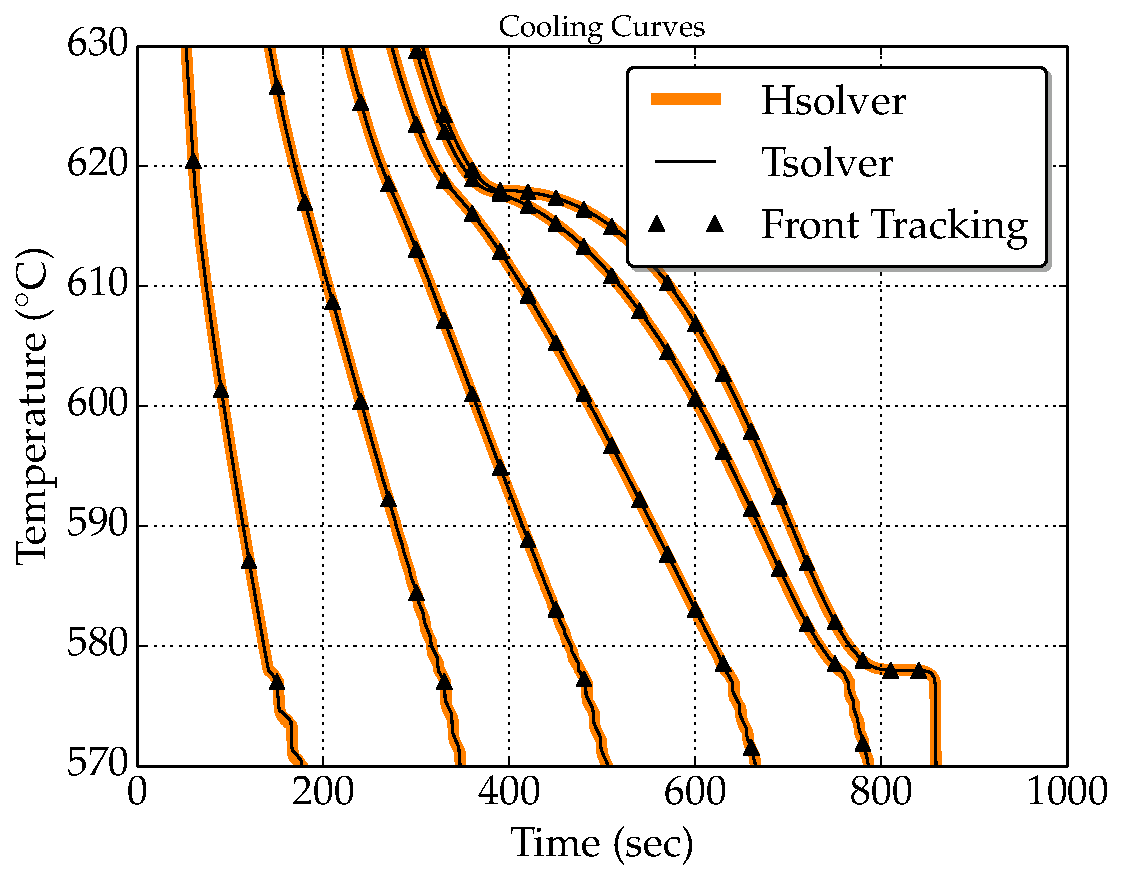
\includegraphics[width=\textwidth]{Chapter3/Graphics/diffusion/diffusion_CC.pdf}
	\caption{}
    \label{fig:validation_diffusion_CC}
  \end{subfigure}
  %------------------------------
  \vskip\baselineskip
  %------------------------------
  \begin{subfigure}[t]{0.7\textwidth}
    \centering
	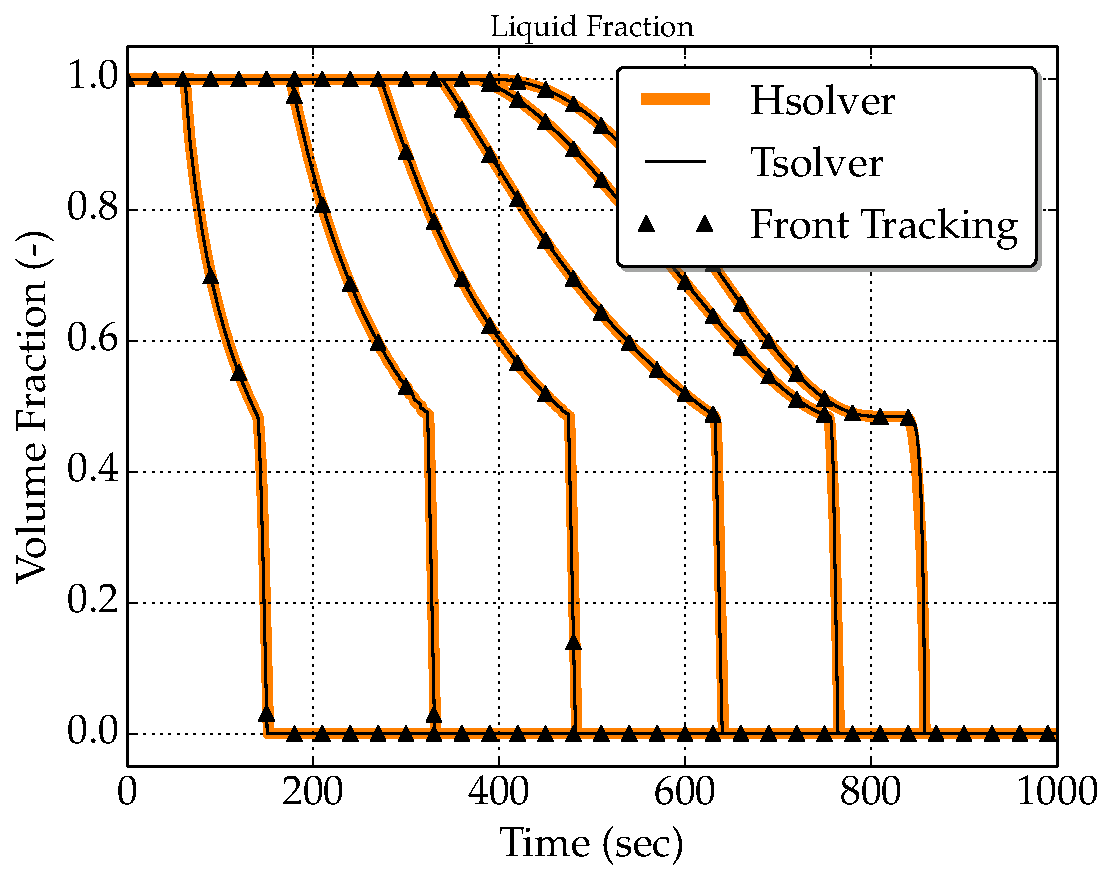
\includegraphics[width=\textwidth]{Chapter3/Graphics/diffusion/diffusion_LF.pdf}
	\caption{}
    \label{fig:validation_diffusion_LF}
  \end{subfigure}
   %------------
\caption{Computed unidirectional heat diffusion during solidification of an \bin{Al}{7}{Si} alloy 
using (orange) the enthalpy method and (black) the temperature method, comparison being made 
for (a) cooling curves  and (b) the liquid fraction history. 
Each curve corresponds to a position along the sample, from 0 cm (cooling 
side) to 10 cm (insulated side), with 2 cm spacing between the positions.
The reference solution by the Front Tracking method (values in shown by the triangular markers).} 
\label{fig:validation_diffusion}
\end{figure}
%------------------


%\subsection{Convection and diffusion}


\section{Application: multicomponent alloy solidification}
%==================
%
We have shown that the efficiency of the temperature-based resolution resides in its performance when combined with 
thermodynamic tabulations. A multicomponent alloy consists of at least two solute elements, and 
therefore the tabulation size increases, hence the number of search operations also increases. 
To demonstrate the speed-up ability of the temperature-based approach while predicting all phase 
transformations during macrosegregation caused solely by mass diffusion, we consider the solidification of a ternary alloy, \tern{Fe}{2}{C}{30}{Cr}.
In order to neglect fluid flow resolution, we assume that solidification in this case is so slow that no forces are generated inside the melt, while
additionally all buoyancy forces are also neglected, so no momentum conservation is solved in this section.

As illustrated in \cref{fig:mutlicomponent_geo}, the alloy domain has a cylinder shape close to 3-inch height $\times$ 1-inch diameter. 
Exact values are reported in \cref{table:ternary_data_case} with all material properties, initial and boundary conditions, 
as well as numerical parameters for the simulations. The steel melt is initially at \SI{1395}{\udegC}. The 
temperature of the bottom surface is imposed with a constant decreasing rate of \SI{0.1}{\uCR} starting 
with \SI{1380}{\udegC} as shown in \cref{fig:mutlicomponent_bc}, i.e. \SI{40}{\udegC} higher than the nominal liquidus temperature as shown 
in \cref{fig:ternary_nominalpath}. The other surfaces are kept adiabatic. 

The cylinder is held in a vertical position parallel to the gravity vector, the latter pointing downwards.
\cref{fig:ternary_nominalpath} also provides the transformation path of the alloy at nominal composition, i.e. assuming no macrosegregation and full 
thermodynamic equilibrium as computed with ThermoCalc and the TCFE6 database \citep{tcfe6_tcfe6:_2010, andersson_thermo-calc_2002}. 
A total of 5 phases need to be handled, the characteristic temperature for their formation being reported 
in \cref{fig:mutlicomponent_bc}.

%-----------------
\begin{figure}[htbp]
\centering
   %------------
  \begin{subfigure}[t]{1.0\textwidth}
    \centering
	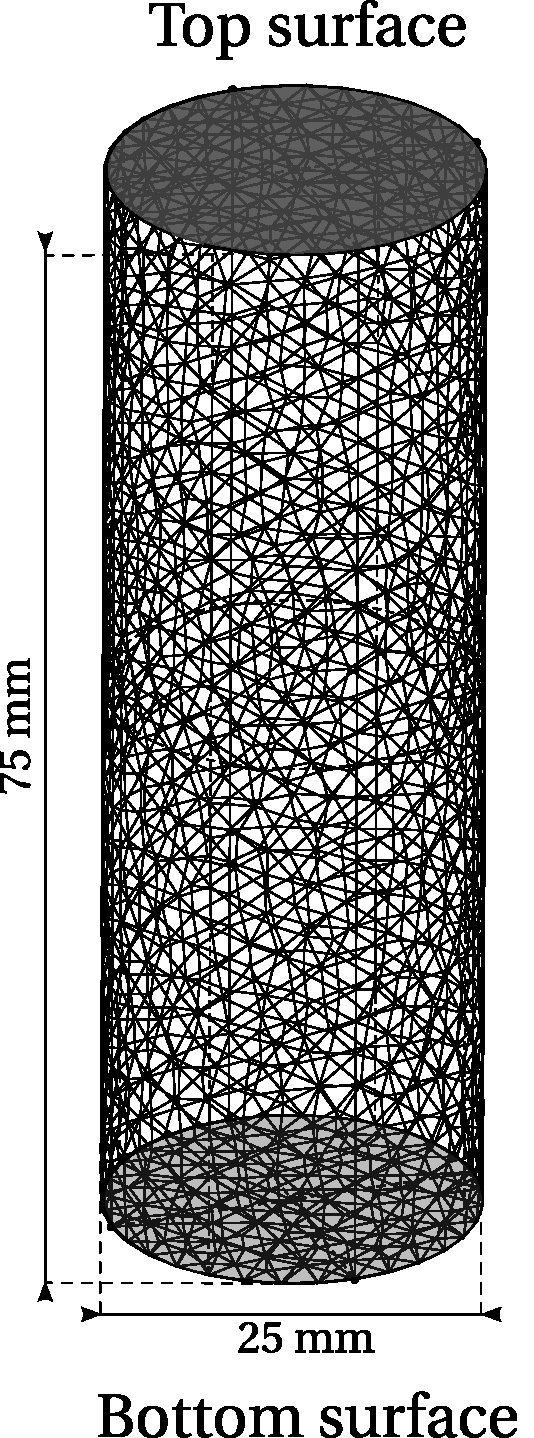
\includegraphics[width=0.25\textwidth]{Chapter3/Graphics/multicomponent/geo_bc/Cylinder_nocolor_annotate.pdf}
	\caption{}
    \label{fig:mutlicomponent_geo}
  \end{subfigure}
   %------------
    \vskip\baselineskip
   %------------
   \hspace{1mm}%\quad
   \begin{subfigure}[t]{1.0\textwidth}
    \centering
	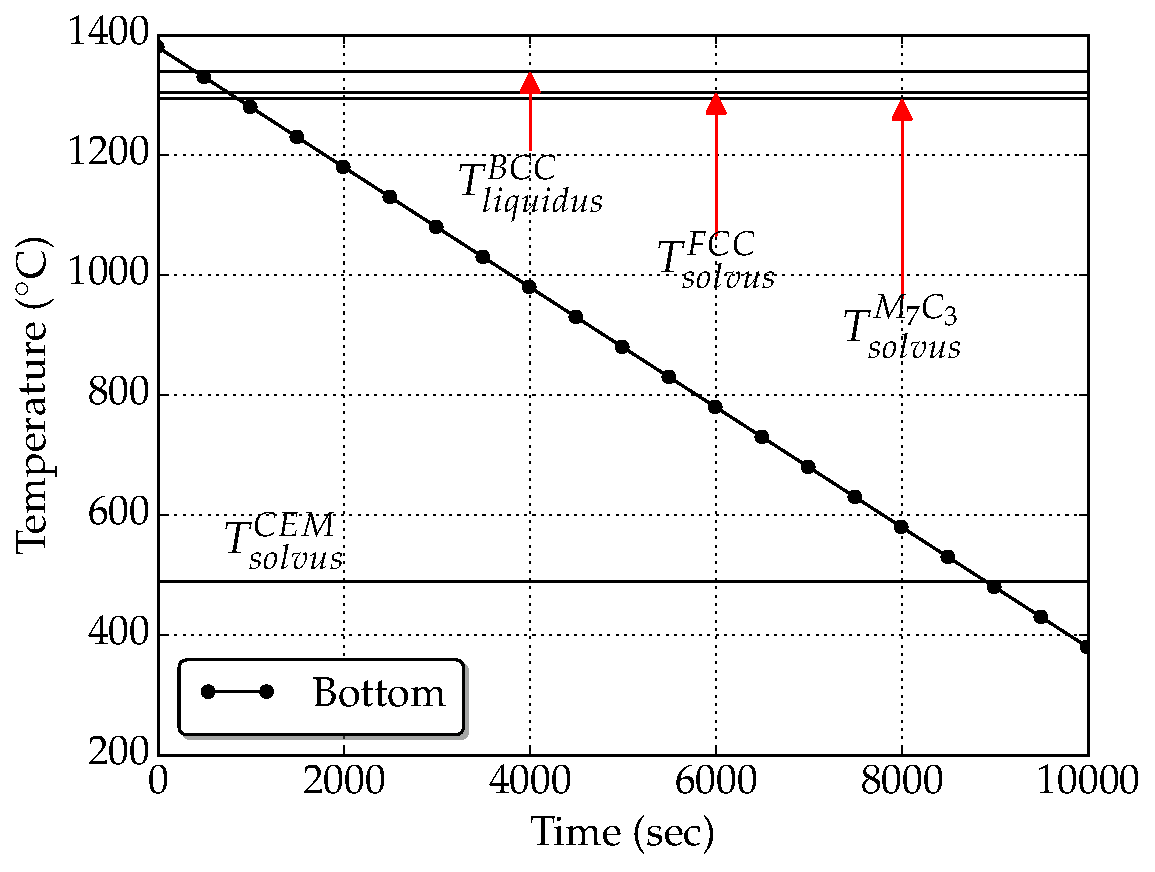
\includegraphics[width=0.75\textwidth]{Chapter3/Graphics/multicomponent/geo_bc/BC.pdf}
	\caption{}
    \label{fig:mutlicomponent_bc}
  \end{subfigure}
  %------------------------------
\caption{Configurations for upward directional casting of (a) a 1-inch diameter $\times$ 3-inches height cylindrical domain for which
(b) temperature-time conditions are imposed at its bottom surface.} 
\label{fig:mutlicomponent_geobc}
\end{figure}
%-----------------melt

%-------------------------
\subsection{Tabulations}
%-------------------------

Full thermodynamic equilibrium is considered in the present case. Due to macrosegregation, 
the average composition is expected to continuously vary in time and space during casting. 
Transformation paths are thus determined a priori for a set of average compositions around 
the nominal value. Hence, carbon content varies in the interval [\SI{1.8}{\ucomposition}, \SI{2.2}{\ucomposition}] 
while chromium content variation is in the interval [\SI{27}{\ucomposition}, \SI{33}{\ucomposition}]. The offset of $\pm$ 10\%  with 
respect to the nominal composition value allows tabulating relatively small composition steps
to ensure a fairly accurate mapping when compared to the corresponding ternary phase diagram. 

The average composition step is \SI{0.04}{\ucomposition} for carbon and \SI{0.6}{\ucomposition} for chromium, thus representing 2\% 
intervals with respect to the nominal composition. The temperature varies in the interval 
[\SI{100}{\udegC}, \SI{1600}{\udegC}] by \SI{5}{\udegC} steps. For each triplet (carbon content 
in \si{\ucomposition} C, ${w_\text{C}}_0$ , chromium content in \si{\ucomposition} Cr,  ${w_\text{Cr}}_0$, temperature in \si{\udegK}) 
corresponds a phase fraction $g^\phi$ and a pair of intrinsic phase composition ($\wC^\phi$,$\wCR^\phi$), $\phi$ representing a phase. For the 5 
phases listed in \cref{fig:ternary_nominalpath} (LIQ$\equiv$liquid, BCC$\equiv$ferrite, FCC$\equiv$austenite, 
$\carbide \equiv$carbide, CEM$\equiv$cementite), the enthalpy $\hphi$ and density $\rphi$, are tabulated 
as functions of temperature and phase intrinsic composition. If this latter input lies between two tabulated 
values, a linear interpolation is performed to determine the output, i.e. phase enthalpy and density. With 
the advancement of solidification, the liquid is enriched or depleted with solute by macrosegregation, which enables new 
solidification paths. It means that the primary solidifying phase is not necessarily the same as when considering 
the nominal composition. For this reason, the tabulation approach is interesting inasmuch as it provides phase 
transformation paths and values of phase properties that are compatible with the system’s actual composition. 

\Cref{fig:ternary_tabulations} summarises the tabulated thermodynamic data for two sets of average composition for the considered 
ternary system. Note that in the present test case, phase densities are taken constant ($\rhos=\rhol=$ \SI{6725}{\udensity}). 
Therefore they are not tabulated. With this assumption, no shrinkage occurs upon phase change.


%----------------------
\begin{figureth}
% textwidth 
{0.8}
%path 
{Chapter3/Graphics/multicomponent/SP_nominal.pdf}
% caption
{Thermodynamic mapping \citep{tcfe6_tcfe6:_2010, andersson_thermo-calc_2002} of the transformation 
path for the \tern{Fe}{2}{C}{30}{Cr} at nominal composition.}
% label
\label{fig:ternary_nominalpath}
\end{figureth}
%-----------------------------------


%=====================================BIG PORTRAIT FIGURE =====================================
\begin{figureth}
% textwidth 
{0.7}
%path 
{Chapter3/Graphics/multicomponent/tabulations/planche_tabulations_portrait.pdf}
% caption
{Tabulated thermodynamic data for the ternary system Fe-C-Cr alloy with software 
Thermo-Calc \citep{andersson_thermo-calc_2002}  with database TCFE6 \citep{tcfe6_tcfe6:_2010}.
The two columns represent two values of average composition, for a) low carbon and chromium content
and b) high carbon and chromium content.
The effect of their variation on transformation paths, phase compositions and phase enthalpies is shown in the corresponding graphs.}
% label
\label{fig:ternary_tabulations}
%\thispagestyle{headings}
\end{figureth}
%=====================================BIG PORTRAIT FIGURE =====================================



%----------------
\begin{tabulate}
%
% caption 
{Solidification parameters for the \tern{Fe}{2}{C}{30}{Cr} alloy.}
% label
{table:ternary_data_case}
% line separation (e.g. 1.5mm)
{0.6mm}
% column justification-number (e.g. |c|ll|)
{llll}
% header titles (should use the & sign to switch columns)
{\textbf{Parameter} & \textbf{Symbol} & \textbf{Value} & \textbf{Unit}}
% cells content (should use the & and // to switch columns and rows)
{
Nominal composition 			& ${w_\text{C}}_0$ 				& 2 					& \si{\ucomposition} 	\\ 
                    			& ${w_\text{Cr}}_0$ 			& 30 					& \si{\ucomposition} 	\\ 
Characteristic temperatures 	& $T_\text{bottom}$ 	& \cref{fig:mutlicomponent_bc}	 & \si{\udegC} \\ 
Phase fraction 					& $g^\phi$ 				& Tabulations \cref{fig:ternary_tabulations}	& $-$ 					\\ 
Phase enthalpy 					& $\h^\phi$ 			& Tabulations \cref{fig:ternary_tabulations}	& $-$ 					\\ 
Phase composition 				& $\wC^\phi$ 			& Tabulations \cref{fig:ternary_tabulations}	& \si{\ucomposition}  	\\ 
Phase composition               & $\wCR^\phi$ 			& Tabulations \cref{fig:ternary_tabulations}	& \si{\ucomposition}  	\\ 
Diffusion coefficients 			& $\avg{D_\text{C}}^l$ 	& \num{15e-10} 	& \si{\udiffusivity}  	\\ 
                        		& $\avg{D_\text{Cr}}^l$	 & \num{15e-10} 	& \si{\udiffusivity}  	\\ 
Dynamic viscosity  				& $\mul$ 					& \num{2e-3} 		& \si{\uviscosity}  	\\ 
Thermal expansion coefficient 	& \betaT 					& \num{8.96e-5} 	& \si{\ubetaT}  		\\ 
Solutal expansion coefficient 	& $\betawlC$ 				& \num{1.54e-3} 	& \si{\ubetawl}  		\\  
                              	& $\betawlCR$ 				& \num{1.72e-2} 	& \si{\ubetawl}  		\\ 
Thermal conductivity in the solid & $\ks$ 					& \num{40} 			& \si{\uconductivity}  	\\ 
Thermal conductivity in the liquid & $\kl$ 					& \num{28} 			& \si{\uconductivity}  	\\ 
Dendrite arm spacing 			& $\lambda$ 				& \num{60e-6} 		& \si{\metre}  			\\ 
Density 						& $\rholref$ 						& \num{6725} 	& \si{\udensity}  		\\ 
Reference composition (carbon)	&$\avg{w_\text{C}}_\text{ref}^l$	& \num{2} 		& \si{\ucomposition}  	\\
Reference composition (chromium)&$\avg{w_\text{Cr}}_\text{ref}^l$	& \num{30} 		& \si{\ucomposition}  	\\
Reference temperature 			&$\avg{w_\text{C}}_\text{ref}^l$	& \num{1377} 	& \si{\udegC}  	\\
\hline 
Initial temperature 	& $T_0$ & \num{1395}	& \si{\udegC}  \\ 
Ingot diameter 			&   	& \num{25e-3} 	& \si{\metre}  \\ 
Ingot length 			&   	& \num{75e-3} 	& \si{\metre}  \\ 
\hline 
FE mesh size 			&  		& \num{e-3} 	& \si{\metre}  \\ 
Time step 				& $\dt$ & \num{0.1} 	& \si{\second}  \\ 
Convergence criterion (residual) 	& $\varepsilon_R$ & \num{e-6} & $-$ \\ 
Convergence criterion (temperature) & $\varepsilon_T$ & \num{e-2} & \si{\udegK} 
}
%
\end{tabulate}
%-----------------


\subsection{Discussion}
%-----------------------
A first case is considered without macrosegregation, that is, all mechanical driving forces are bypassed, leading to a static melt. 
This is achieved by nullifying the thermal and solutal expansion coefficients, which is equivalent to a constant density in space 
and time, i.e. no Boussinesq force is considered. This way, the average composition may only vary due to diffusion in the liquid 
phase.
%according to \cref{eq:diag_solute} where the convection term is neglected. 

Diffusion is significantly small in the present case and can be 
neglected too. The composition distribution thus maintains a homogeneous aspect throughout the sample during the entire 
cooling sequence. The phase transformations then are necessarily expected to follow the unique path shown in \cref{fig:ternary_nominalpath}. After 407 s 
of cooling, the liquidus isotherm enters the bottom surface of the geometry and starts its upward propagation, marking the solidification 
onset. 

\Cref{fig:planche_nomacroseg} presents the simulation results at 3 successive times for the distribution of the solute species and the temperature, as 
well as for the fraction of phases listed in \cref{fig:ternary_nominalpath}. At 600 s, a fully liquid region is still largely present while the mushy zone is 
made of liquid plus the primary solid phase (ferrite). At \num{10560} s, the sample is fully solid, with fractions of ferrite and cementite that 
corresponds to the values read in \cref{fig:ternary_nominalpath} at low temperature. At the selected intermediate time, the presence of 4 phases is found. The 
solid region at the bottom of the cylinder is made of ferrite, austenite plus carbide, the temperature being still too high to permit the 
cementite to form. The mushy zone above the solid region is characterized by the presence of 3 phases due to a peritectic reaction taking 
place that progressively transforms ferrite into austenite in the presence of liquid. 

It can be noticed that the phase fraction isovalues 
in \cref{fig:planche_nomacroseg} (at 600 s) are horizontal, owing this to two factors: the first is the temperature field, which varies unidirectionally from 
bottom to top, controlled by thermal diffusion, while the second is the uniform average composition throughout the sample due to the absence 
of convection. In fact both factors are consequences of the flow absence, which would transport heat and solute by advection, thus inevitably 
changing the phase distribution. The succeeding phase change is a solid-state transformation where $\alpha$-ferrite and the carbide $\carbide$ react to form 
cementite after cooling below \SI{490}{\udegC}, as shown in \cref{fig:mutlicomponent_bc}. The reaction is relatively slow, ending with 28\% 
of cementite and 72\% of $\alpha$-ferrite.

%=====================================BIG LANDSCAPE FIGURE =====================================
\begin{landscape}
\begin{figureth}
{1.2}
{Chapter3/Graphics/multicomponent/planche_nomacroseg.pdf}
{Upward solidification of a cylinder rod with a static liquid at 
3 stages in a \tern{Fe}{2}{C}{30}{Cr}. The left columns show the average 
composition and temperature distribution, while the right columns show the phase fractions.}
\label{fig:planche_nomacroseg}
%\thispagestyle{headings}
\end{figureth}
\end{landscape}
%=====================================BIG LANDSCAPE FIGURE =====================================

\section{Limitations}

The \emph{Tsolver} method is well suited for 
solidification problems with macrosegregation. In this chapter, only pure diffusion cases were simulated. 
The next chapter discusses the details of solving Navier-Stokes equations while predicting macrosegregation, 
showing thus the advantage of using the thermodynamic tabulation approach with the \emph{Tsolver}.
However, some limitations are still present and need to be explained.

First, we address the technical difficulties inherent to the solver. The previously shown algorithm in \cref{fig:TsolverSteps},
showed that the Newton-Raphson method is used to linearise the energy equation then iterate on the value of the nonlinear
$\vec{\dHdT}$ term. The initial value of this term is crucial to achieve a good convergence rate, and therefore it is only manually set equal 
to initial phases volume heat capacity. This should evolve into an automatic initialisation based on a first evaluation given by the tabulation,
making the appraoch more general. 

The second point is the number of iterations needed by the method to converge.
Although the Newton-Raphson algorithm is known for its quadratic convergence speed, imposing low convergence thresholds (\cref{eq:energy_convergence_criteria}) 
may easily raise the number of iterations to an average of 5 iterations before convergence can be achieved. In situations without
phase change but only variable slope of enthalpy versus temperature, from 1 to 2 iterations are needed to converge.
A possible solution is to implement a line search method which is called at each iteration, whenever the residual of the nonlinear
system increases insteading of steadily decreasing. 
% Moreover, since $\vec{dHdT}$ is a derivative which is based on ratio of finite differences for averaged volumetic enthalpy and temperature, \red{continue...}

Regarding the thermodynamic tabulations, they are only obtained by assuming full equilibrium for macrosegregation calculations. 
For many binary alloys, little differences are usually seen when the macrosegregation is induced by a full equlibrium and a non equilibrium solidification
It is clear however that this approximation remains limiting for multicomponent alloys. 
For steels, a third type of approximation is even required, named partial equilibrium, that considers equal chemical potential 
of interstitial elements in all phases (e.g., C), while substitutional species in the solid phases (e.g., Cr) are frozen \citep{koshikawa_computation_2014}. 




\clearpage
\section*{Résumé chapitre 3}

Ce chapitre reprend les détails du solveur pour la conservation d'énergie avec changement de phase utilisé au CEMEF.
Celui-ci est basé sur une méthode enthalpique, dénommée \emph{Hsolver}, dont la variable principale est l'enthalpie
moyenne volumique du système, $\avg{\rho h}$. Ce solveur est aussi compatible avec des données tabulées provenant de bases de données
thermodynamiques, fournissant des valeurs précises pour chaque phase $\phi$ présente au moment de la transformation: 
fraction $\gphi$, composition intrinsèque $\wiphi$, enthalpie massique $\hphi$ et densité $\rphi$. 
Avec ces données, l'équation de conservation de l'énergie est résolue dans son état nonlinéaire 
provenant de la dépendance de $\rho h$ par rapport aux propriétés citées précédemment, sachant que celles-ci varient
aussi en fonction de la composition moyenne du volume élémentaire représentatif.


Cependant, la résolution \emph{Hsolver} nécessite une lourde recherche itérative à chaque pas de temps, consistant à convertir
$\avg{\rho h}$ en température $T$ pour évaluer le résidu du système nonlinéaire. Cette conversion est dénommée \emph{H2T} et elle est
compliquée du fait que les bases thermodynamiques fournissent la température comme donnée d'entrée, ce qui nous oblige de faire 
la recherche inverse itérative.


Dans ce chapitre, on propose de remplacer la conversion \emph{H2T} par une autre, \emph{T2H}. Comme son nom l'indique,
on part de l'idée que la température soit la variable principale du système et on devrait alors trouver l'enthalpie moyenne volumique
à chaque pas de temps. Avec ce changement, on propose donc une nouvelle formulation éléments finis, \emph{Tsolver}, mettant en évidence les principales
différences algorithmiques des deux résolutions.


Nous validons la formulation \emph{Tsolver} dans un cas purement diffusif et comparé à des calculs faits avec la méthode \emph{Hsolver}, 
ainsi qu'une comparaison avec une solution numérique obtenue par une méthode de suivi de front \citep{gandin_constrained_2000}.
Enfin, nous montrons une application de solidification dirigée d'un système ternaire, \tern{Fe}{0.2}{C}{30}{Cr}, en régime diffusif.

% avec une analyse de la ségrégation en peau et en coeur de la pièce. % resume francais
 % Coupling with Fluid Mechanics I: Monodomain
\chapter{Macrosegregation with solidification shrinkage}
%\chaptermark{Nonlinear Temperature Solver}
\begin{nolinkcolors} 
\minitoc
\end{nolinkcolors}
\newpage

this chapter discusses the following points:
\begin{itemize}
\item Density variation during solidification (industrial point of view then how to handle numerically)
\item Model equations
\item Application to solidification benchmark SMACS
\item Possible extension of application with grain structure (using Shijia's LS-air cells handling)
\item Multiscale Freckle predicition: FE + grain structure (in which lies a part about nucleation-growth and how numerically 
		we reach a smaller scale, the scale of the grain boundaries)
\end{itemize}

% ======================
\section{Literature review}
% ======================
Solidification shrinkage is, by definition, the effect of relative density change between the liquid and solid phases.
In general, it results in a progressive volume change during solidification, until the phase change has finished. 
The four stages in \Cref{fig:real_ingot_stage_a,fig:real_ingot_stage_c,fig:real_ingot_stage_b,fig:real_ingot_stage_d} depict the volume change with 
respect to solidification time.
First, at the level of the first solid crust, near the local solidus temperature, the solid forms with a density smaller than 
the liquid's. This does not necessarily apply for all materials, but at least for steels it does. The subsequent volume difference 
tends to create voids with a big negative pressure, that needs to be compensated by a surrounding fluid. It thus drains 
the liquid metal in its direction (cf. \autoref{fig:real_ingot_stage_b}). As a direct result of the inward feeding flow, the ingot surface
tends to gradually deform in the feeding direction, forming the so-called \emph{shrinkage pipe}. Since the mass of the alloy and its 
chemical species is conserved, a density difference between the phases ($\rhol < \rhos \implies \frac{\rhol}{\rhos}<1$) eventually leads 
to a different overall volume ($V^s<V^l$) once solidification is complete, as confirm the following equations:
\begin{subequations}
\begin{align}
& \rhol V^l = \rhos V^s  \\ 
& V^s = \frac{\rhol}{\rhos} V^l
\end{align}
\end{subequations}
%=============
\begin{figure}[h!] %h!
\centering
%\begin{minipage}{.5\textwidth}
  \begin{subfigure}{0.3\textwidth}
    \centering
    \def\svgwidth{100pt}
	\import{Chapter4/Graphics/new/}{ingot_air_liq.pdf_tex}
	\caption{Initial state}
    \label{fig:real_ingot_stage_a}
  \end{subfigure}
  %\hfill
  \begin{subfigure}{0.3\textwidth}
    \centering
    \def\svgwidth{100pt}
	\import{Chapter4/Graphics/new/}{ingot_air_liq_mush_sol.pdf_tex} 
	\caption{Early intermediate state}
    \label{fig:real_ingot_stage_b}
  \end{subfigure}
%
\vskip\baselineskip
%======
%
  \begin{subfigure}{0.3\textwidth}
    \centering
    \def\svgwidth{100pt}
	\import{Chapter4/Graphics/new/}{ingot_air_mush_sol.pdf_tex}
	\caption{Late intermediate state}
    \label{fig:real_ingot_stage_c}
  \end{subfigure}
  %\hfill
  \begin{subfigure}{0.3\textwidth}
    \centering
    \def\svgwidth{100pt}
	\import{Chapter4/Graphics/new/}{ingot_air_sol.pdf_tex}
	\caption{Final state}
    \label{fig:real_ingot_stage_d}
  \end{subfigure}
  %
\caption{Schematic of the main cooling stages of an ingot against side and bottom mould walls (not shown)}
\label{fig:real_ingot_stages}
\end{figure}
\comment{ \textbf{Sutaria2012} talk about feeding paths, but more importantly they computed thermal shrinkage WITHOUT solving
NavierStokes equations. To predict the interface shape, they solve a LS transport with an imposed velocity given by Gada et Sharma 2009}

%====================================================================
\section{Level set treatment}

\subsection{Permeability mixing}
How to mix liquid fraction, best using harmonic or arithmetic, in order to replicate the effect the of non slip condition at top for example \\
Put the python plots from the presentations in "TEXUS monolithic" \\
Put video animations of PSEUDO SMACS 2D without and with LS ???



%====================================================================
\section{Conservation equations}

\subsection{Mass Conservation}
% ======================
\subsubsection{Assumptions}
% ======================
\begin{itemize}
\item Two phases are considered, liquid $l$ and solid $s: \gl+\gs =1 $ % \implies \frac{dg^l}{dt} =- \frac{dg^s}{dt}$ 
\item The phase densities are constant but not equal: $ \rhol=cst_1 $ and $ \rhos=cst_2 $. Thermal and solutal expansion/contraction
is neglected
\item The solid phase is assumed static: $\vec{v^s}=\vec{0}$, which yields the following consequences:
\begin{enumerate}
\item $ \avg{\vec{v}}= \gl \vec{v^l} + \cancelto{0}{\gs \vec{v}^s} = \gl \vec{v}^l $
\item $ \avg{\rho \vec{v}} = \gl \rhol \vec{v}^l + \cancelto{0}{\gs \rhol \vec{v}^s} = \gl \rhol \vec{v}^l $
\item $\nabvec \rhol = \nabvec \rhos = \vec{0}$
\end{enumerate}
\end{itemize}
% ======================
\subsubsection{Formulation}
% ======================
The mass balance equation averaged over the two phases, is expanded taking into account the aforementioned assumptions.
\begin{subequations}
\begin{align}
& \frac{\partial \avg{\rho}}{\partial t} + \nabla \cdot \avg{\rho \vec{v}}  = 0 \\ 
& \frac{\partial }{\partial t} \brac{ \gl \rhol + \gs \rhos} + \nabla \cdot \brac{ \gl \rhol \vec{v}^l} = 0 \\ 
& \gl \cancel{\frac{\partial \rhol }{\partial t}} + \rhol \frac{\partial  \gl }{\partial t} 
	+ \gs \cancel{\frac{\partial \rhos }{\partial t}} + \rhos \frac{\partial  \gs }{\partial t} 
	+ \rhol \nabla \cdot \brac{ \gl \vec{v}^l} 
	+ \gl \vec{v}^l \cdot  \cancel{ \nabvec \rhol }	 = 0 \\
& \brac{ \rhol - \rhos } \frac{\partial  \gl }{\partial t} + \rhol \nabla \cdot \brac{ \gl \vec{v}^l}  = 0
\end{align}
\end{subequations}
\begin{align}
\label{eq:mass_balance}
 \boxed{\nabla \cdot \brac{ \gl \vec{v}^l} 
 	= \nabla \cdot \avg{\vec{v}^l} 
 	= \frac{\rho^l-\rho^s}{\rho^l} \frac{\partial  \gs }{\partial t}}
\end{align}
% ======================
\subsubsection{Discussion}
% ======================
With the assumptions of static solid phase and constant unequal phase densities, the average mass balance states that 
the divergence of the liquid velocity is proportional to the solidification rate, the proportionality constant being the
relative density change (which results in a relative volume change). This relation between the liquid velocity and the
temporal derivative of the solid fraction, explains the flow due to shrinkage. In metallic alloys, the solid density is
usually greater than the liquid density, therefore the first term in the RHS is negative. As for the second term, if we
neglect remelting, then it'll be positive in the solidifying areas of the alloy. A negative divergence term in these areas, 
means that a liquid feeding is necessary to compensate for the density difference, hence acting as a flow driving force in the melt.
In the case of constant densities, we can easily deduce that the divergence term is null, and therefore no flow is induced
by solidification.
\newline
Numerically speaking, a non-zero divergence term in the mass balance is equivalent to a compressible fluid behaviour. Additional 
terms should appear in the other conservation equations, balancing the volume change in the momentum, heat and species transport.

%====================================================================
\subsection{Momentum Conservation}
% ======================
In a typical volume averaging approach, one would write one momentum conservation 
equation for each phase. Nonetheless, only one equation will be present in our case, 
and that is the consequence of the assumption of the static solid, made in the previous 
section. It should be emphasized that, despite considering a single conservation equation, 
the effect of the solid movement with respect to the liquid's can still be incorporated 
through the interfacial fluxes in the momentum conservation of the liquid phase. 
% ======================
\subsubsection{Assumptions}
% ======================
\begin{itemize}
%%%
\item The interfacial momentum transfer between the solid and liquid phases is modelled 
by a momentum flux vector $\vec{\Gamma}^{l}$, consisting of hydrostatic and deviatoric 
parts, such that:
\begin{subequations}
\begin{align}
\label{eq:eq_interfacial_momentum_init}
		& \vec{\Gamma}^{l} =  \vec{\Gamma}_{p}^{l} + \vec{\Gamma}_{\mathbb{S}}^{l}						\\
		& \vec{\Gamma}_{p}^{l} = p^{l^{*}} \nabvec g^{l} = p^{l} \nabvec g^{l}			  \\
		& \vec{\Gamma}_{\mathbb{S}}^{l} = -{g^{l}}^{2} \mu^{l} \mathbb{K}^{-1} \brac{ \vl - \cancel{\vs} }  
\end{align}
\end{subequations}
where $p^{l^{*}}$ is the pressure at the interface, considered to be equal to the liquid hydrostatic 
pressure, $\mathbb{K}$ is the permeability computed by the Carman-Kozeny relation and $\mu^l$ is the 
liquid's dynamic viscosity.  For the solid phase, the interfacial terms are the opposite, which cancels 
them out with the liquid terms if the phase momentum equations are summed up.
%%%
\item The liquid is considered as a \emph{compressible} Newtonian fluid. It implies that the deviatoric part, $\mat{\mathbb{S}}^{l} $, of the Cauchy 
stress tensor is decomposed as follows: 
\comment{CAG: the liquid is incompressible, but the mixture is compressible, change it}
\begin{subequations} 
\begin{align}
\label{eq:stress_liq}
& \avg{ \mat{\sigma}^{l} } = - \avg{p^l} \mat{\mathbb{I}} + \avg{\mat{\mathbb{S}}^{l}}   \\
& \avg{ \mat{\sigma}^{l} } = - \avg{p^l} \mat{\mathbb{I}} + 2\mu^{l} \strainrate + \avg{\mat{\tau}^l}
\end{align}
\end{subequations}
where $ \avg{{\dot{\mat{\varepsilon}}}^l} $ is the strain rate tensor that depends on the average liquid velocity: 
\begin{align}
\label{eq:tensor_strainrate}
\strainrate = \mat{\nabla} \vit  +  \mat{\nabla}^\text{\textbf{t}} \vit 
\end{align}
and  $\mat{\tau}^{l}$ is the extra stress tensor in the liquid, given by:
\begin{subequations}
\begin{align}
\label{eq:tensor_extrastress}
 & \avg{\mat{\tau}^l} =  -\lambda \nabla \cdot \vit  \mat{\mathbb{I}} 
\end{align}
\end{subequations}
where $\lambda$ is a dilatational viscosity \textbf{CITE RAP2003}. For an incompressible flow, the divergence term vanishes, hence the classical Newtonian constitutive law is retrieved. In the literature, the coefficient $\lambda$ is taken proportional to the viscosity: $\lambda = \frac{2}{3} \mu^l $
\end{itemize}
% ======================
\subsubsection{Formulation}
% ======================
The momentum conservation equation in the liquid writes:
\begin{align}
\label{eq:momentum_liq}
& \temp{\rho^l \gl \vec{v}^l } + \nabvec \cdot \brac{\rho^l \gl \vl \times \vl} = 
	\nabvec \cdot \brac{\gl \mat{\sigma}^l} + \gl \vec{F}_\text{v} + \vec{\Gamma}^{l}
\end{align}
where $\vec{F}_\text{v}$ is an external volume force. The effect of the mass balance obtained in the previous section 
is incorporated by expanding the temporal and spatial derivatives in the momentum equation, taking firstly the left-hand side of equation \eqref{eq:momentum_liq}.
\begin{subequations}
\begin{align}
\label{eq:momentum_liq_LHS_a}
	 \text{LHS} &=
	 \rhol \temp{ \gl \vl } + \gl \vl \cancel{\frac{\partial \rhol}{\partial t}} 
	+ \vl \nabla \cdot \brac{ \rhol \gl \vl } 
	+ \nabmat \vl \brac{ \rhol \gl \vl } \\
\label{eq:momentum_liq_LHS_b}
	&= \rhol \underbrace{ \temp{ \gl \vl } }_{\substack{\text{Unsteady} \\ \text{Acceleration}}}
	 + \brac{ \rhol - \rhos } \underbrace{ \frac{\partial  \gs }{\partial t} \vl}
	    _{\substack{\text{Shrinkage}\\ \text{Acceleration}}}
	+ \rhol  \underbrace{ \nabmat \vl \brac{ \gl \vl }}_{\substack{\text{Advective} \\ \text{Acceleration}}}     
\end{align}
\end{subequations}
The development in \eqref{eq:momentum_liq_LHS_b} shows that the origin of the flow, namely its acceleration, is 
attributed to three causes: 
 i) unsteady acceleration: a temporal change of a particle's velocity, ii) shrinkage-induced acceleration: a local "suction" effect at the solid-liquid interface (where $\frac{\partial  \gs }{\partial t} >0$) caused by the density jump $\brac{ \rhol - \rhos }$
and iii) convective acceleration: a spatial change in the velocity field.
The effect of the \emph{shrinkage-induced} flow is introduced using the mass balance in equation \eqref{eq:mass_balance}. The right-hand side of equation \eqref{eq:momentum_liq} is now expanded:
\begin{subequations}
\begin{align}
\label{eq:momentum_liq_RHS}
	\text{RHS} 
	&=
	 \nabvec \cdot \brac{\avg{p^l} \mat{\mathbb{I}} + 2\mu^{l} \strainrate + \avg{\mat{\tau}^l}} 
	 + \gl \rhol \vec{g} 
	 + \vec{\Gamma}_{p}^{l} + \vec{\Gamma}_{\mathbb{S}}^{l}	 \\
	&=  -\nabvec \brac{\gl p^l} 
		+ \nabvec \cdot \brac{ 2 \mu^l \strainrate }
		+ \nabvec \cdot \brac{-\frac{2}{3} \mu^l \nabla \cdot \avg{\vl} \mat{\mathbb{I}}}
		+ \gl \rhol \vec{g} 
	 	+ \vec{\Gamma}_{p}^{l} + \vec{\Gamma}_{\mathbb{S}}^{l}	 \\
	&=  \cancel{- p^l \nabvec \gl} - \gl \nabvec p^l
		+ \nabvec \cdot \brac{ 2 \mu^l \strainrate }
		+ \nabvec \cdot \brac{-\frac{2}{3} \mu^l \nabla \cdot \avg{\vec{v}^l} \mat{\mathbb{I}}}
		+ \gl \rhol \vec{g} 
	 	+ \cancel{\vec{\Gamma}_{p}^{l}} + \vec{\Gamma}_{\mathbb{S}}^{l}	 \\
	&=   - \gl \nabvec p^l
		+ \nabvec \cdot \brac{ \mu^l \brac{\mat{\nabla} \avg{\vec{v}^l} + ^\text{\textbf{t}} \mat{\nabla} \avg{\vec{v}^l} }}
		+ \nabvec \brac{-\frac{2}{3} \mu^l \frac{\rho^l-\rho^s}{\rho^l} \frac{\partial  \gs }{\partial t} }
		+ \gl \rhol \vec{g} 
	 	- {\gl}^{2} \mu^l \mathbb{K}^{-1} \vec{v}^{l}
\end{align}
\end{subequations}
The system thus consists of 3 equations (one for each of the components of $\vec{v}^l$) and 4 unknowns ($\vec{v}^l_x$, $\vec{v}^l_y$, $\vec{v}^l_z$ and $p$). An additional equation is provided by the mass continuity equation \eqref{eq:mass_balance}. For convenience, the superficial velocity $\vit$ will be chosen as a velocity unknown instead of the intrinsic average: $\vit = \gl \vec{v}^l$. The final system to 
solve, after grouping the unknowns in the LHS and the remaining terms in the RHS, is given by:
\comment{ I changed \emph{split} to \emph{align} here }
%\begin{empheq}[box=\widefbox, left=\empheqlbrace]{align}
\label{eq:momentum_liq_final}
%\label{eq:momentum_liq_final_vitesse}
\begin{align} % split
& \rhol \frac{\partial \vit}{\partial t}
	 + \frac{ \rhol - \rhos }{\gl}\frac{\partial  \gs }{\partial t} \vit
	 + \rhol  \nabmat \vl \vit
	 + \nabvec \cdot \brac{2 \mu^l \strainrate}
	 + \gl \mu^l  \mathbb{K}^{-1} \vit  \\
	 &\qquad  = \gl \nabvec p^l
	 + \nabvec \brac{-\frac{2}{3} \mu^l \nabla \cdot \avg{\vec{v}^l}  }
	 +  \gl \rhol \vec{g}  \\
%\label{eq:momentum_liq_final_pression}
&\nabla \cdot \vit= \frac{\rho^l-\rho^s}{\rho^l} \frac{\partial  \gs }{\partial t}
\end{align} % split
%\end{empheq}
%\end{subequations}

%====================================================================
\subsection{Energy Conservation}
% ======================
We have seen the averaged energy conservation equation in the case of two phases: a solid phase and an incompressible liquid phase. However, with the incorporation of the shrinkage effect, new terms should appear
in the advective-diffusive heat transfer equation. 
% ======================
\subsubsection{Assumptions}
% ======================
\begin{itemize}
\item The thermal conductivity is constant for both phases: $\avg{\kappa} = \ks = \kl= \kappa $ 
%\item consideration of a fixed solid ($ \vec{v}^s=\vec{0} $).
\item Consequence of the static solid phase: $\avg{\rho h \vec{v}} = \gl \rhol \hl \vl +  \cancel{\gs \rhos \hs \vs} = \gl \rhol \hl \vl$ 
\item The system's enthalpy may thermodynamically evolve with pressure, knowing that $h=e+\frac{p}{\rho}$, where $e$ is the internal energy and $p$ is the pressure. It infers that the heat transport
equation may contain a contribution attributed to volume compression/expansion:
\begin{align}
			 \frac{\partial p}{\partial t}+\nabla \cdot \brac{p \vec{v}}
			 = \frac{\partial p}{\partial t}+ p \nabla \cdot \vec{v} + \vec{v} \cdot \nabvec p 
\end{align}
In the literature, this contribution has been always neglected, even when accounting for solidification
shrinkage, owing to the small variations of pressure.
\item Another contribution is also neglected in solidification problems, that is the heat generated by
mechanical deformation, $\mathbb{S}:\dot{\varepsilon}$ 
%\begin{enumerate}
%\item $\avg{\rho h}= \gl \rhol \hl + \gs \rhos \hs $
%\end{enumerate}
\end{itemize}
% ======================
\subsubsection{Formulation}
% ======================
The unknowns in the energy conservation are the average volumetric enthalpy $\avg{\rho h}$ and temperature $T$.The energy conservation equation writes:
\begin{subequations}
\begin{align}
	& \frac{\partial \avg{\rho h}}{\partial t} + \nabla \cdot \avg{\rho h \vec{v}} 
	= \nabla  \cdot \brac{\avg{\kappa} \nabvec T } \\
	& \frac{\partial \avg{\rho h}}{\partial t} + \nabla \cdot \brac{\gl \rhol \hl \vl}
	= \nabla  \cdot \brac{\kappa \nabvec T } \\ 
	& \frac{\partial \avg{\rho h}}{\partial t} 
		+ \rhol \hl  \nabla \cdot \vit
		+ \vit \cdot \nabvec \brac{\rhol \hl}
		= \nabla  \cdot \brac{\kappa \nabvec T } \\   
	& \frac{\partial \avg{\rho h}}{\partial t} 
		+ \cancel{\rhol} \hl  \frac{\rhol-\rhos}{\cancel{\rhol}} \frac{\partial  \gs }{\partial t}
		+ \vit \cdot \nabvec \brac{\rhol \hl}
		= \nabla  \cdot \brac{\kappa \nabvec T } \\ 
	& \frac{\partial \avg{\rho h}}{\partial t} 
		+ \brac{\rhol-\rhos} \hl \frac{\partial  \gs }{\partial t}
		+ \vit \cdot \nabvec \brac{\rhol \hl}
		= \nabla  \cdot \brac{\kappa \nabvec T }        
\end{align}
\end{subequations}
\begin{align}
\label{eq:energy_balance}
 \boxed{ \frac{\partial \avg{\rho h}}{\partial t} 
		+ \rhol \vit \cdot \nabvec \hl
		= \nabla  \cdot \brac{\kappa \nabvec T }
		+ \brac{\rhos-\rhol} \hl \frac{\partial  \gs}{\partial t}}
\end{align}

% ======================
\subsubsection{Discussion}
% ======================
In order to keep things simple, the term "enthalpy" will refer henceforth to "volume enthalpy",
otherwise, we will explicitly use the term "mass enthalpy". It is important to understand the 
meaning of the terms in equation \eqref{eq:energy_balance}.
The first term in the left-hand side is the temporal change in the system's average enthalpy,
i.e. a temporal change in the volume enthalpy of any of the phases in the course of solidification.
The second LHS term is a dot product between the superficial liquid velocity and the the gradient
of the liquid's enthalpy. Since phase densities are constant in our case, the gradient term reduces
to the liquid's mass enthalpy. If we consider a representative volume element (RVE) in the liquid
phase, far from the mushy zone, we can stipulate:
\begin{align}
\label{eq:gradient_liquid_enthalpy}
& \nabvec \hl = C_p^l \nabvec T
\end{align}
assuming that the phase mass specific heat, $ C_p^l $, is constant. Therefore, the liquid enthalpy
is advected in the case where the velocity vector is not orthogonal to the temperatre gradient.
The advection reaches its maximum when the two vectors have the same direction. Consider, for instance,
a filled ingot with a cooling flux applied to its bottom surface. If the density variation with temperature
were to be neglected, then the sole mechanical driving force in the melt is the density jump at the solid-liquid
interface ahead of the mushy zone. The temperature gradient in such a case is vertical upward, while the velocity
vector is in the opposite direction. The advective term writes:
\begin{align}
%\label{eq:}
& \rhol \vit \cdot \nabvec \hl = - \rhol C_p^l \norm{\vit} \norm{\nabvec T}
\end{align}
% FIGURE %%
\begin{figure}
\centering
\begin{subfigure}[h!]{0.3\textwidth}\centering % h! or H
	\def\svgwidth{100pt}
	\import{Chapter4/Graphics/}{Ingot_sl_1D_a.pdf_tex}
	\caption{Initial state}
	\label{fig:ingot_1d_a}
\end{subfigure}
\begin{subfigure}[h!]{0.3\textwidth}\centering % h! or H
	\centering
	\def\svgwidth{100pt}
	\import{Chapter4/Graphics/}{Ingot_sl_1D_c.pdf_tex}
	\caption{Solidification onset}
	\label{fig:ingot_1d_c}
\end{subfigure}
\begin{subfigure}[h!]{0.3\textwidth}\centering % h! or H
	\centering
	\def\svgwidth{100pt}
	\import{Chapter4/Graphics/}{Ingot_sl_1D_d.pdf_tex}
	\caption{Final state}
	\label{fig:ingot_1d_d}
\end{subfigure}
\caption{Effect of shrinkage flow on a solidifying ingot}
\end{figure}
%% FIGURE %%
We see that the second RHS term in equation \eqref{eq:energy_balance} acts as 
a heat source at the interface between the the phases, in this particular solidification
scenario. Another heat power (of unit $Wm^{-3}$) adds to the system within the mushy, 
that is the second term in the right-hand side of the same equation. This term is 
proportional to the solidification rate. Finally, the first RHS term accounts for thermal 
diffusion within the phases.
\newline
It should be emphasized that the assumption of a constant specific heat in the liquid in 
equation \eqref{eq:gradient_liquid_enthalpy} applies when no macrosegregation occurs. 
Nonetheless, when the latter is considered, the phases specific and latent heats become 
highly dependent on the local average composition. It then advisable to use the thermodynamic 
tabulation approach, where the enthalpies are directly tabulated as functions of temperature 
and composition. 
% ======================
\subsection{Species Conservation}
% ======================
The last conservation principle is applied to the chemical species or solutes. This principle allows predicting
macrosegregation when applied to a solidification system, along with the mass, momentum and energy balances.
However, the conservation equation should be reformulated in the case of a melt flow driven by shrinkage.
% ======================
\subsubsection{Assumptions}
% ======================
\begin{itemize}
\item The alloy is binary, i.e., it is composed from one solute, and hence the notation of the average composition
		without a solute index: $\wavg$ for the mass composition and $\avg{\rho w}$ for the volume composition
\item The solid fration is determined assuming complete mixing in both phases, hence the lever rule is applicable. It
		should be mentionned that the solidification path in the current approach is tabulated using thermodynamic data at 
		equilibrium
\item The solutal diffusion coefficient $D^s$ in the solid phase is neglected in the mass diffusive flux term. The
		remaining term, $D^l$, is a mass diffusion coefficient in the liquid phase, of unit $m^2 s^{-1}$
\item Consequence of the static solid phase: $\avg{\rho w \vec{v}} = \gl \rhol \wl \vl +  \cancel{\gs \rhos \ws \vs} = \gl \rhol \wl \vl$ 
\end{itemize}
% ======================
\subsubsection{Formulation}
% ======================
The species conservation is pretty similar the energy conservation formluted in the previous section. For a binary alloy, we can write:
\begin{subequations}
\begin{align}
	& \frac{\partial \avg{\rho w}}{\partial t} + \nabla \cdot \avg{\rho w \vec{v}} 
	= \nabla  \cdot \brac{\rhol \avg{D^l} \nabvec \wl } \\
	& \frac{\partial \avg{\rho w}}{\partial t} + \nabla \cdot \brac{\gl \rhol \wl \vl}
	= \nabla  \cdot \brac{\gl\rhol D^l \nabla \wl } \\ 
	& \frac{\partial \avg{\rho w}}{\partial t} 
		+ \rhol \wl  \nabla \cdot \vit
		+ \vit \cdot \nabvec \brac{\rhol \wl}
		= \nabla  \cdot \brac{\gl \rhol D^l \nabvec \wl } \\   
	& \frac{\partial \avg{\rho w}}{\partial t} 
		+ \cancel{\rhol} \wl  \frac{\rhol-\rhos}{\cancel{\rhol}} \frac{\partial  \gs }{\partial t}
		+ \vit \cdot \nabvec \brac{\rhol \wl}
		= \nabla  \cdot \brac{\gl \rhol D^l \nabvec \wl } \\ 
	& \frac{\partial \avg{\rho w}}{\partial t} 
		+ \brac{\rhol-\rhos} \wl \frac{\partial  \gs }{\partial t}
		+ \vit \cdot \nabvec \brac{\rhol \wl}
		= \nabla  \cdot \brac{\gl \rhol D^l \nabvec \wl }        
\end{align}
\end{subequations}
\begin{align}
\label{eq:solute_balance}
 \boxed{ \frac{\partial \avg{\rho w}}{\partial t} 
		+ \rhol \vit \cdot \nabvec \wl
		= \nabla  \cdot \brac{\rhol D^l \nabvec \wl }
		+ \brac{\rhos-\rhol} \wl \frac{\partial  \gs}{\partial t}}
\end{align}
% ======================
\subsubsection{Discussion}
% ======================
The species transport equation is usually derived with the volumetric average composition $\avg{\rho w}$, then
divided by the density, which is constant if no solidification shrinkage occurs. In the case where macrosegregation
is solely due to fluid flow generated by natural or forced convection, the overall
volume remains constant. It is thus convenient to compute composition variations using the mass variable $\wavg$.
However, in the current context, the volume is subject to changes, hence the formulation of equation 
\eqref{eq:solute_balance} with $\avg{\rho w}$.

\section{Test cases}

\subsection{Validation of LS transport}
\comment{perform test case simulation of buyoancy driven air droplet in water by 2005Nagrath that I also have seen 
in Shyamprasad's masters report)}
\comment{ I read it quickly without noticing: what time step $\delta t$ did they use ? }

\subsection{Shrinkage without macrosegregation}
Smacs or Pseudo-Smacs test case with Level set and shrinkage
\subsubsection{Considerations}
Explain how the flow and heat transfer in the air are not important \\ 
\subsubsection{Model equations}
Give the strong form equations to be solved OR simply refer the previous section where the model was defined
\subsubsection{Initial and boundary conditions for energy and momentum}
Initially we have liquid and air at rest. 
\subsubsection{Results and discussion}

 % Coupling with Fluid Mechanics II: Level Set Approach
\chapter{Macrosegregation with solidification shrinkage}
%\chaptermark{Nonlinear Temperature Solver}
\begin{nolinkcolors} 
\minitoc
\end{nolinkcolors}
\newpage

% ======================
\section{Solidification shrinkage}
% ======================

Solidification shrinkage is, by definition, the effect of relative density change between the liquid and solid phases.
In general, it results in a progressive volume change during solidification, until the phase change has finished. 
The four stages in \cref{fig:real_ingot_stage_a,fig:real_ingot_stage_c,fig:real_ingot_stage_b,fig:real_ingot_stage_d} depict the volume change with 
respect to solidification time.
First, at the level of the first solid crust, near the local solidus temperature, the solid forms with a density greater than 
the liquid. The subsequent volume decrease forces the fluid to be sucked in the direction of the volume change 
(cf. \cref{fig:real_ingot_stage_b}). 
When this sucking becomes impossible due to a low permeability of the mush, voids may appear.
As a direct result of the inward feeding flow, the ingot free surface with the air
tends to gradually deform to follow the feeding direction, forming the so-called \emph{shrinkage pipe}, shown in \cref{fig:shrinkage_exp}. 
Since the mass of the alloy and its chemical species is conserved, 
a density difference between the phases ($\rhol < \rhos \implies \frac{\rhol}{\rhos}<1$) eventually leads 
to a different overall volume ($V^s<V^l$) once solidification is complete, as confirm the following mass conservation equations, 
from initial (LHS term) to final (RHS term) state:
%------------
\begin{subequations}
\begin{align}
& \rhol V^l = \rhos V^s  \\ 
& V^s = \frac{\rhol}{\rhos} V^l
\end{align}
\end{subequations}
%------------
Solidification shrinkage is not the only factor responsible for volume decrease. 
Shrinkage due to temperature and composition variations in both solid and liquid phases, are also common causes in a casting process. 
Thermal shrinkage is very important to apprehend in steel casting, as the temperature decrease usually exceeds a \SI{1000}{\udegC} between the solidus and ambient temperature.
This causes substantial density variations. 
%Henceforth, we will focus on shrinkage due to phase change.
%
%Talk and explain models in the literature that predict shrinkage (without or with macrosegregation): Beckermann, Wu ? \\
%Show and comment the experiments that have been done: Hebditch and Hunt, Smacs Hachani  ...
%
%\comment{ \textbf{Sutaria2012} talk about feeding paths, but more importantly they computed thermal shrinkage WITHOUT solving
%NavierStokes equations. To predict the interface shape, they solve a LS transport with an imposed velocity given by Gada et Sharma 2009}
%
%
%----------------
%
\begin{figure}[htbp]
\centering
%\begin{minipage}{.5\textwidth}
  \begin{subfigure}[t]{0.25\textwidth}
    \centering
    \def\svgwidth{80pt}
	\import{Chapter5/Graphics/new/}{ingot_air_liq.pdf_tex}
	\caption{Initial state}
    \label{fig:real_ingot_stage_a}
  \end{subfigure}
  %\hfill
  \begin{subfigure}[t]{0.25\textwidth}
    \centering
    \def\svgwidth{80pt}
	\import{Chapter5/Graphics/new/}{ingot_air_liq_mush_sol.pdf_tex} 
	\caption{Early intermediate state}
    \label{fig:real_ingot_stage_b}
  \end{subfigure}
%
\vskip\baselineskip
%======
%
  \begin{subfigure}[t]{0.25\textwidth}
    \centering
    \def\svgwidth{80pt}
	\import{Chapter5/Graphics/new/}{ingot_air_mush_sol.pdf_tex}
	\caption{Late intermediate state}
    \label{fig:real_ingot_stage_c}
  \end{subfigure}
  %\hfill
  \begin{subfigure}[t]{0.25\textwidth}
    \centering
    \def\svgwidth{80pt}
	\import{Chapter5/Graphics/new/}{ingot_air_sol.pdf_tex}
	\caption{Final state}
    \label{fig:real_ingot_stage_d}
  \end{subfigure}
  %
\caption{Schematic of the main cooling stages of an ingot against side and bottom mould walls (not shown)}
\label{fig:real_ingot_stages}
\end{figure}
%
%---------------------
%
%----------------------
\begin{figureth}
% textwidth 
{0.45}
%path 
{Chapter5/Graphics/shrinkage_exp.png}
% caption
{Sulphur prints of three low-carbon steel ingots showing pipe formation at the top as a result 
of solidification shrinkage, marked with dark areas corresponding to higher sulphur content, while varying ingot inclination during casting.
Ingot orientation changes from (a) vertical position to (b) \SI{25}{\degree}-inclination after 34 minutes of vertical (dashed line) casting and finally (c) \SI{25}{\degree}-inclination after 3 hours of vertical casting. The white arrow indicates the inclination onset \citep{onodera_effect_1959}. The black arrow indicates the gravity direction.}
% Positive macrosegregation is clearly seen in this area, while A-shape and V-shape positive mesosegregates are detected
% at the ingot's tips and centre respectively.
% label
\label{fig:shrinkage_exp}
\end{figureth}
%-----------------------------------
%
%
%============================================
\section{Choice of boundary tracking}
%============================================
In chapter 2, several methods of boundary tracking/capturing methods were presented 
along with their similarities and differences. In the case of solidification shrinkage,
the metal-air boundary can be tracked with any method from the previously mentioned.
However, several reasons motivate us to settle on the level set method. 
First, the easiest solution is testing a method which already exists in the \cimlib library.
The level set method was implemented as a framework for monolithic resolution. Since this work,
the method has been extensively used and improved in several projects mainly for multiphase flows, which is the 
main competence of the Computing and FLuids (C.FL.) group at CEMEF. Another motivation is the compatibility
between \cimlib and \thercast, where the latter is the final destination of the code developed during this Ph.D. thesis.
In its recent versions, \thercast handles laminar and turbulent ingot filling where the level set method is used 
to capture the free surface of the molten metal. Aside from the practical motivations, some technical aspects of the level
set method make it very attractive to address macroscopic surface tracking 
(in contrast to microscopic interface tracking, for instance the solid-liquid interface), 
such as topological properties that are readily available (e.g. curvature)
and accurate position compared to volume-based methods like VOF \citep{sethian_level_1999}.
%
%============================================
\section{Multidomain formalism}
%============================================
In the previous chapters, we considered in our simulations the metallic alloy as a 
saturated mixture of solid and liquid during solidification.
It means that no gas phase was supposed to appear during the process.
Additionally, we ignored shrinkage and expansion effects. These considerations
resulted in a fixed interface between the free surface of the liquid metal and the surrounding air.
As a consequence, air was not considered in the model.
The reason is that we chose to describe our model in Eulerian description, 
for which we have considered a fixed grid to discretise the averaged conservation 
equations governing the phase change between the liquid and solid phases.
With the introduction of shrinkage, an increase in global density of the metallic alloy means 
that a gas phase should enter the domain to replace the shrunk volume.

At this point, several interfaces may be distinguished: liquid-solid ($l$-$s$), liquid-air ($l$-$a$) and solid-air ($s$-$a$), where 
we defined 2 phases ($l$ and $s$) belonging to the "Metal" domain denoted $M$, while the "Air" domain, denoted $A$, 
is made up of a unique gas phase, ($a$), with the same name. As a standard for this formalism, we consider that upper case letters
are used for domains, while lower case letters are used for phases.

The main idea behind the multidomain formalism is to go from the classic 
conservations equations introduced by volume averaging in chapter 2
in the context of a solidifying two-phase system to generalise it by taking
into account a third gas phase, such as:
%-------------
\begin{align}
\label{eq:}
V^l + V^s + V^a = \rev \\
\gl + \gs + \ga = 1
\end{align} 
%-------------
where $\gphi$ is the volume fraction of each phase $\phi=[l,s,a]$.
Then, one is free to choose a suitable numerical method to define and track the 
physical interfaces between the several phases. In our macroscale applications, we are particularly 
interested in keeping an indirect representation of the $l$-$s$ interface (dotted line in \cref{fig:rev_triphase})
using the volume averaging theory, while employing a different
method to track the metal-air ($M$-$A$) boundary ($l$-$a$ and $s$-$a$ interfaces, represented by dashed lines in \cref{fig:rev_triphase}) with the level set method. 
This allows switching to the latter method in a physically representative manner.

In this context, each domain can be seen as a material having a physical
interface with the other domains. As a consequence of our interpretation, 
the gas phase should not exist in the metal, which may naturally
occur if the thermodynamic conditions are in favour of nucleating and growing 
a new phase, or in the case of a gas that was trapped inside mould grooves.
%----------------------
\begin{figureth}
% textwidth 
{0.45}
%path 
{Chapter5/Graphics/REV_triphase.pdf}
% caption
{Schematic of a representative volume element containing 3 phases with distinct velocities, separated by 3 interfaces.
The dotted line is the indirectly tracked solid-liquid interface while the other dashed lines, air-liquid and air-solid
interfaces, are directly tracked.}
% label
\label{fig:rev_triphase}
\end{figureth}
%-----------------------------------

\subsection{Assumptions}
%------------
Each phase in the system has its own velocity, $\vl$, $\vs$ and $\va$, while the respective
interfaces $\liqsol$, $\liqair$ and $\solair$ have different and independent velocities, 
represented by $\vliqsol$, $\vliqair$ and $\vsolair$. Note that the solid-liquid interface
velocity was denoted $\vstar$ in the previous chapters as no more than two phases were considered.

The first major assumption is that the solid phase, once formed from the liquid, is fixed and rigid, hence $\vs=\vec{0}$.
It means that no subsequent deformation or contraction/expansion of the solid phase ($\rhos=\text{constant}$) may occur and therefore $\vsolair$ reduces to vector zero.
Moreover, we use the already introduced volume averaging principles to write locally for any quantity $\psi$:
%------------
\begin{subequations}
\begin{align}
\label{eq:}
\avg{\psi} &= \avg{\psi^l} \avg{\psi^s} + \avg{\psi^a} \\
			&= \gl \psi^l + \gs \psi^s  + \ga \psi^a
\end{align}
\end{subequations}
%------------
where volume fractions, $\gphi$, for each phase $\phi$ were used. \citet{rappaz_numerical_2003} define
the volume fraction by writing a general expression inside the representative volume $\rev$:
%------------
%\begin{subequations}
\begin{align}
\label{eq:}
\gphi = \frac{1}{\rev} \integral{\rev}{\chi^\phi(x,t)}{\Ohm} = \avg{\chi^\phi}
\end{align}
%\end{subequations}
%------------
where the integrated quantity is an indicator (or presence) function relative to phase $\phi$, which
defines the volume of this phase in the system, $\Ohm^\phi$, as follows:
%------------
%\begin{subequations}
\begin{align}
\label{eq:}
\chi^\phi(x,t)=
\begin{cases}
  1 	& \text{ if } x \in \Ohm^\phi \\ 
  0 	& \text{otherwise}
\end{cases}
\end{align}
%\end{subequations}
%------------
Any phenomenon that may displace an interface, whether by phase change or a phase motion, is 
mathematically translated by variations of the presence function, such that its total derivative for each phase
satisfies the following:
%
%------------
\begin{align}
\label{eq:transport_presence}
& \frac{d \chi^\phi}{dt} = \tempup{\chi^\phi} + \vstar \cdot \nabvec \chi^\phi = 0
\end{align}
%------------
%
If we consider the liquid phase for instance, the variations of any quantity $\psi$ are given by:
%------------
\begin{align}
\label{eq:variations1}
& \avg{{\tempup{\psi^l}}} = \tempup{\avg{\psi^l}}
							- \frac{1}{\rev} \integral{\Gamma_{l-a}}{\psi^l \vliqair \cdot \nliqair}{A}
							- \frac{1}{\rev} \integral{\Gamma_{l-s}}{\psi^l \vliqsol \cdot \nliqsol}{A} \\
\label{eq:variations2}
& \avg{\nabvec \psi^l} =  \nabvec{\avg{\psi^l}} 
							+ \frac{1}{\rev} \integral{\Gamma_{l-a}}{\psi^l \nliqair}{A} 
							+\frac{1}{\rev} \integral{\Gamma_{l-s}}{\psi^l \nliqsol }{A} \\
\label{eq:variations3}
& \avg{\nabvec \cdot \vec{\psi}^l} =  \nabvec \cdot {\avg{\vec{\psi}^l}} 
							+ \frac{1}{\rev} \integral{\Gamma_{l-a}}{\vec{\psi^l} \cdot \nliqair }{A} 
							+\frac{1}{\rev} \integral{\Gamma_{l-s}}{\vec{\psi^l} \cdot  \nliqsol }{A}							
\end{align}
%------------

So far, we know that \cref{eq:transport_presence} allows transporting an interface between 2 phases, 
or a more generally a boundary between multiphase domains.
We also know that \cref{eq:variations1,eq:variations2,eq:variations3} allow computing temporal and spatial
variations of any physical quantity related to a phase or more generally a multiphase domain.
To avoid ambiguity, we still have to establish a definition for the boundary between the metal and the air, i.e. which 
interfaces should be accounted for when considering the transport of the metal-air boundary.



\subsection{Metal-Air boundary definition} 
%---------------------------------------------

% ---------------BEGINNING OF INSERTED TEXT ----------------------------------
In reality, between the metal and the air, two boundaries exist, as explained by \citet{niane_etude_2004}. 
% the liquid-air ($\liqair$) and solid-air ($\solair$) interfaces, 
% and these interfaces move at different velocities as solidification proceeds.
The liquid-air interface exists at early stages of solidification where only the free surface of the liquid is in contact with the air, as shows stage 1 in  \cref{fig:1dalsi7_interface_stages}.
% In this case, the metal-air boundary is defined by the $\liqair$ interface, where the latter is driven by solidification shrinkage, 
% and therefore by 

In later stages (transition from stage 2 to stage 3 in \cref{fig:1dalsi7_interface_stages}), the mushy zone delimited by dendrite tips, 
reaches the free liquid surface, creating hence two distinct boundaries: 
a first boundary separating interdendritic liquid from the air, and a second boundary that separates the dendrite tips from the air.
In other words, a porous medium made up of solid+air settles between the mushy zone (solid+liquid) and the air domain. The lower part of the this porous medium is defined by the $\liqair$ interface and is driven by solidification shrinkage.
Therefore, its real microscopic velocity is equal to the interdendritic liquid velocity, $\vl$. 
According to \citet{dantzig_solidification_2009},
this velocity is constant when the solidification shrinkage and the isotherms velocity $\vec{v}_T$ are constant, as states the equation:
%----------------
\begin{align}
\label{eq:real_velocity}
& \vl = -\beta_{SS} \vec{v}_T
\end{align}
%---------------
As for the upper part of porous medium, delimited by the $\solair$ interface, its motion could be induced by a mechanical deformation of the solid phase either due to thermal shrinkage/expansion or external mechanical stresses.
The first factor is ubiquitous in any solidification process, while the second factor is process-dependent. 

In the present work, we remind that the solid phase is assumed fixed and rigid, therefore we consider dendrites to be undeformable during their growth. 
Unfortunately, this assumption is contradictory with our current situation where the metal keeps shrinking, 
until an overlap of the transition zone (intersection of both domains, identified by $\heaviside^{tr}$) and the mushy zone takes place, 
as shown in \cref{fig:1dalsi7_interface_stages} (second row, stage 3).
At this point, both interfaces define the \emph{M-A} boundary. Although it is necessary to track the $\solair$ boundary also, the present work limited to considering the $\liqair$ interface as fully defining the metal-air boundary. 
Tracking the $\solair$ interface adds complexity as an additional tracking method has to be used like a new level set with distinct numerical properties. 
This assumption will have some influence regarding the overall simulation performance, as some errors are induced, as the porous medium is not properly accounted for.
Further discussions about the outcomes of our definition of the metal-air boundary are given in the 1D application section.
% ---------------END OF INSERTED TEXT ----------------------------------
With the previous definitions, \cref{eq:transport_presence} can be recast with the level set 
method by using the smoothed Heaviside function in the metal:
% For the metal, this function is equal to one and decreases to zero in the air in a smooth way across both interfaces, solid-air and liquid-air.
% Since the solid phase is assumed fixed without possible deformation, and knowing that air is assumed incompressible, 
% the solid-air interface does not move, leading to the following equation: 
%------------
\begin{subequations}
\begin{align}
\label{eq:transport_heaviside}
& \frac{d \heavisideM}{dt} = \tempup{\heavisideM} + \vec{v^{M-A}} \cdot \nabvec \heavisideM = 0 \\
& \frac{d \heavisideM}{dt} = \tempup{\heavisideM} + \vliqair \cdot \nabvec \heavisideM = 0
\end{align}
\end{subequations}
%------------

%--------------
\begin{figureth}
% textwidth 
{1.0}
%path 
{Chapter5/Graphics/1d/interface_stages.pdf}
% caption
{Schematic describing (first row) the physical solidification process and (second row) its numerical treatment of moving the boundary between air and metal domains, at three intermediate stages of solidification. 
$\heavisideM$, $\heavisideA$ and $\heaviside^{tr}$ are respectively the Heaviside functions for the metal, the air and the transition zone between both domains.}
% label
\label{fig:1dalsi7_interface_stages}
\end{figureth}
%--------------

%======================

\section{FE partitioned model}
%--------------------------------------------------
 
In this section, we start from the monodomain finite element model 
presented in \cref{sec:monodomain} that was relevant to the metal only, 
referred to by the superscript $M$, then present the essential assumptions and formulations 
that allow predicting solidification shrinkage in a Eulerian context that introduces
another domain, the air, referred to by the superscript $A$.

\subsection{In the metal}
% ------------------------------------------------

\subsubsection{Mass and momentum conservation}
% ------------------------------------------------

By assuming a fixed solid phase ($\vs=\vec{0}$), i.e. a constant density 
for the solid phase without any transport of this phase, 
the average velocity in the metal reduces only to liquid's average velocity. 

Therefore, we can write:
%------------
\begin{align}
\label{eq:vitmetal}
& \vM = \vit + \avg{\vs} = \gl \vl + \cancel{\gs \vs}
\end{align}
%------------

With \cref{eq:vitmetal}, the mass balance in the metal writes:
%------------
\begin{subequations}
\begin{align}
& \tempup{\avg{\rho}^M} + \nabvec \cdot \avg{\rho \vec{v}}^M  = 0 \\ 
& \tempup{\avg{\rho}^M} + \nabvec \cdot \brac{ \gl \rhol \vl} = 0 \\ 
& \tempup{\avg{\rho}^M} + \rhol \nabvec \cdot \brac{ \gl \vl} 
	+ \gl \vl \cdot  \nabvec \rhol = 0 \\	
\label{eq:mass_balance_metal}
& \nabvec \cdot \vit 
= -\frac{1}{\rhol} \brac{\tempup{\avg{\rho}^M }+ \vit \cdot  \nabvec \rhol}
\end{align}
\end{subequations}
%------------

\Cref{eq:mass_balance_metal} explains the flow due to shrinkage. 
A negative divergence term means that a liquid feeding 
is necessary to compensate for a density increase upon solidification, where $\rhos > \rhol$ in the transient term, 
hence acting as a flow driving force in the melt.
The second RHS term accounts for the volume change 
due to heat and species variations in the liquid.

When the metal's density was considered constant during solidification, 
the assumption of an incompressible system made it possible to
use the Boussinesq approximation. However, in the case of solidification shrinkage, 
the average density ${\avg{\rho}}^M$ varies, as it depends on the solidification 
path as well as on $\rhos$ and $\rhol$ which are not equal nor constant.

Therefore, the incompressibility condition is no more applicable. In such case, 
the earlier given system \cref{eq:Navier-Stokes2} is reformulated without 
any reference value for density and assuming a fixed solid phase:
%------
\begin{equation}
\label{eq:momentum_balance_metal}
   \left\{
   \begin{aligned}
      & \rhol \brac{\tempup{ \vit } + \frac{1}{\gl} \nabvec \cdot \brac{\vit \times \vit}} = \\
	  &- \gl\nabvec \pl - 2 \mul \nabvec \cdot \brac{\nabmat \vit + \nabmattransp \vit}
	  - \gl \mul \K^{-1} \vit + \gl \rhol \gravity\\ \\
      & \nabvec \cdot \vit = -\frac{1}{\rhol} \brac{\tempup{\avg{\rho}^M} + \vit \cdot  \nabvec \rhol}
    \end{aligned}
    \right.
\end{equation}
%------------

%====================================================================
\subsubsection{Energy conservation}
% ======================
In the energy equation, a volumetric source term accounts for the heat dissipation 
caused by the shrinking metal volume. Before writing the new equation, we make the following assumptions:

% ======================
%Assumptions
% ======================
\begin{itemize}
\itemsep0em
%\item The thermal conductivity is constant for both phases: $\avg{\kappa} = \ks = \kl= \kappa $ 
%\item consideration of a fixed solid ($ \vec{v}^s=\vec{0} $).
\item consequence of the static solid phase: $\avg{\rho h \vec{v}}^M = \gl \rhol \hl \vl +  \cancel{\gs \rhos \hs \vs}$,
%\item The system's enthalpy may thermodynamically evolve with pressure, knowing that $h=e+\frac{p}{\rho}$, where $e$ is the internal energy and $p$ is the pressure. It infers that the heat transport equation may contain a contribution attributed to volume compression/expansion:
%\begin{align}
%			 \frac{\partial p}{\partial t}+\nabvec \cdot \brac{p \vec{v}}
%			 = \frac{\partial p}{\partial t}+ p \nabvec \cdot \vec{v} + \vec{v} \cdot \nabvec p 
%\end{align}
%In the literature, this contribution has been always neglected, even when accounting for solidification
%shrinkage, owing to the small variations of pressure.
\item the heat generated by mechanical deformation, $\mathbb{S}:\dot{\varepsilon}$, is neglected.
%\begin{enumerate}
%\item $\avg{\rho h}= \gl \rhol \hl + \gs \rhos \hs $
%\end{enumerate}
\end{itemize}
% ======================
%Formulation
% ======================
The unknowns in the energy conservation are the average volumetric enthalpy $\avg{\rho h}^M$ and temperature $T$.
The energy conservation equation writes:
%--------------
\begin{subequations}
\begin{align}
	& \tempup{\avg{\rho h}^M} + \nabvec \cdot \avg{\rho h \vec{v}}^M 
	= \nabvec  \cdot \brac{\avg{\kappa}^M \nabvec T } \\
	& \tempup{\avg{\rho h}^M} + \nabvec \cdot \brac{ \gl \rhol \hl \vl} 
	= \nabvec  \cdot \brac{\avg{\kappa}^M \nabvec T } \\
	& \tempup{\avg{\rho h}^M}
		+ \vit \cdot \nabvec \brac{\rhol \hl}
		= \nabvec  \cdot \brac{\avg{\kappa}^M \nabvec T }
		  - \rhol \hl  \nabvec \cdot \vit \\   
	\label{eq:energy_balance_metal}
	& \tempup{\avg{\rho h}^M}
		+ \vit \cdot \nabvec \brac{\rhol \hl}
		= \nabvec  \cdot \brac{\avg{\kappa}^M \nabvec T }
		+ \hl \brac{\tempup{\avg{\rho}^M} + \vit \cdot  \nabvec \rhol} 
\end{align}
\end{subequations}
%\begin{align}
% \boxed{ \frac{\partial \avg{\rho h}}{\partial t} 
%		+ \rhol \vit \cdot \nabvec \hl
%		= \nabvec  \cdot \brac{\kappa \nabvec T }
%		+ \brac{\rhos-\rhol} \hl \frac{\partial  \gs}{\partial t}}
%\end{align}
%----------------
%
%In order to keep things simple, the term "enthalpy" will refer henceforth to "volume enthalpy",
%otherwise, we will explicitly use the term "mass enthalpy". It is important to understand the 
%meaning of the terms in equation \cref{eq:energy_balance}.
%The first term in the left-hand side is the temporal change in the system's average enthalpy,
%i.e. a temporal change in the volume enthalpy of any of the phases in the course of solidification.
%The second LHS term is a dot product between the superficial liquid velocity and the the gradient
%of the liquid's enthalpy. Since phase densities are constant in our case, the gradient term reduces
%to the liquid's mass enthalpy. If we consider a representative volume element (RVE) in the liquid
%phase, far from the mushy zone, we can stipulate:
%
%--------------
%\begin{align}
%\label{eq:gradient_liquid_enthalpy}
%& \nabvec \hl = C_p^l \nabvec T
%\end{align}
%--------------
%
%assuming that the phase mass specific heat, $ C_p^l $, is constant. Therefore, the liquid enthalpy
%is advected in the case where the velocity vector is not orthogonal to the temperatre gradient.
%The advection reaches its maximum when the two vectors have the same direction. Consider, for instance,
%a filled ingot with a cooling flux applied to its bottom surface. If the density variation with temperature
%were to be neglected, then the sole mechanical driving force in the melt is the density jump at the solid-liquid
%interface ahead of the mushy zone. The temperature gradient in such a case is vertical upward, while the velocity
%vector is in the opposite direction. The advective term writes:
%
%--------------
%\begin{align}
%\label{eq:enthalpy_advection}
%& \rhol \vit \cdot \nabvec \hl = - \rhol C_p^l \norm{\vit} \norm{\nabvec T}
%\end{align}
%--------------
%
%----------------------------
%\begin{figure}
%\centering
%\begin{subfigure}[h!]{0.3\textwidth}\centering % h! or H
%	\def\svgwidth{100pt}
%	\import{Chapter5/Graphics/}{Ingot_sl_1D_a.pdf_tex}
%	\caption{Initial state}
%	\label{fig:ingot_1d_a}
%\end{subfigure}
%\begin{subfigure}[h!]{0.3\textwidth}\centering % h! or H
%	\centering
%	\def\svgwidth{100pt}
%	\import{Chapter5/Graphics/}{Ingot_sl_1D_c.pdf_tex}
%	\caption{Solidification onset}
%	\label{fig:ingot_1d_c}
%\end{subfigure}
%\begin{subfigure}[h!]{0.3\textwidth}\centering % h! or H
%	\centering
%	\def\svgwidth{100pt}
%	\import{Chapter5/Graphics/}{Ingot_sl_1D_d.pdf_tex}
%	\caption{Final state}
%	\label{fig:ingot_1d_d}
%\end{subfigure}
%\caption{Effect of one-dimensional shrinkage flow on a solidifying ingot}
%\end{figure}
%----------------------
%
%We see that the second LHS term in equation \eqref{eq:energy_balance} acts as 
%a heat source at the interface between the the phases, in this particular solidification
%scenario. 

The second term in the RHS of \cref{eq:energy_balance_metal} is a heat power (of unit $Wm^{-3}$) 
that adds to the system in the liquid phase (if $\rhol$ is not constant) as well as in the mushy zone (if $\rhol$ and $\rhos$ are not equal). 
This term is proportional to the solidification rate and expresses 
the heat generated in regions where the average density is changing and/or a gradient of liquid density is being advected.

% ======================
\subsubsection{Species conservation}
% ======================
The last conservation principle is applied to the chemical species or solutes. This principle allows predicting
macrosegregation when applied to a solidification system, along with the mass, momentum and energy balances.
However, the conservation equation should be reformulated in the case of a melt flow driven by shrinkage.
% ======================
% Assumptions
% ======================
Considered assumptions are: 
\begin{itemize}
\itemsep0em
%\item the alloy is binary, i.e. it is composed from one solute, and hence the notation of the average composition
%		without a solute index: $\wavg$ for the mass composition and $\avg{\rho w}$ for the volume composition
\item %the solid fraction is determined assuming complete mixing in both phases, hence the lever rule is applied. 
	  the solidification path is tabulated using thermodynamic data at equilibrium,
\item the macroscopic solute diffusion coefficient $D^s$ in the solid phase is neglected in the mass diffusive flux term,
\item consequence of the static solid phase: $\avg{\rho w \vec{v}}^M = \gl \rhol \wl \vl +  \cancel{\gs \rhos \ws \vs}$.
\end{itemize}

% ======================
%Formulation
% ======================
The species conservation presents similarities with the energy conservation formulated in the previous section. 
The main difference is the breakup of the volumetric variable $\avg{\rho w}^M$ into a product of 
density  $\avg{\rho}^M$ and the mass composition $\avg{w}^M$ in the transient term.

For a binary alloy, we write:
%--------------------------
\begin{subequations}
\begin{align}
 & \tempup{\avg{\rho w}^M} + \nabvec \cdot \avg{\rho w \vec{v}}^M - \nabvec  \cdot \brac{\avg{\Dl} \nabvec \brac{\rhol \wl} } = 0 \\
 %
 & \avg{\rho}^M \tempup{\avg{w}^M} + \avg{w}^M \tempup{\avg{\rho}^M} 
	+ \nabvec \cdot \brac{\gl \rhol \wl \vl} 
	- \nabvec \cdot \brac{\gl \Dl \nabvec \brac{\rhol \wl} } = 0 \\
 %
 \label{eq:species_1}
  \begin{split}
	& \avg{\rho}^M \tempup{\avg{w}^M} + \avg{w}^M \tempup{\avg{\rho}^M} 
	+ \brac{\rhol \wl} \nabvec \cdot \vit + \vit \cdot \nabvec \brac{\rhol \wl} \\
	& - \nabvec \cdot \brac{\gl \Dl \nabvec \brac{\rhol \wl} } = 0 
  \end{split}
%
\end{align}
\end{subequations}
%--------------------------

The mass balance, \cref{eq:mass_balance_metal}, gives the following relation when the liquid density is constant:
%--------------------------
\begin{align}
\label{eq:species_divV}
\nabvec \cdot \vit = -\frac{1}{\rhol} \brac{\tempup{\avg{\rho}}^M}
\end{align}
%----------------
If we use the result of \cref{eq:species_divV} in \cref{eq:species_1}, then we get the following equation:
\begin{align}
\avg{\rho}^M \tempup{\avg{w}^M}  + \avg{w}^M \tempup{\avg{\rho}^M} =
\wl \tempup{\avg{\rho}^M}  - \vit \cdot \nabvec \brac{\rhol \wl} + \nabvec \cdot \brac{\gl \Dl \nabvec \brac{\rhol \wl} }
\end{align}
%
Applying Voller-Prakash \citep{voller_modelling_1989} variable splitting, the system ends up with only one variable, $\avg{w}^M$. 
The splitting is done as follows:
\begin{align}
\label{eq:voller_prakash}
\wl = \brac{\wl}^t + \avg{w}^M - \brac{\avg{w}^M}^t
\end{align}
%
where the superscript $t$ refers to the previous time step, and the absence 
of this superscript corresponds to the unknown variable at the next time step.
The chemical species conservation writes, still assuming a constant liquid density:
%
% \begin{subequations}
\begin{align}
  \begin{split}
	& \avg{\rho}^M \tempup{\avg{w}^M}  + \cancel{\avg{w}^M \tempup{\avg{\rho}^M}} = \\
	& \cancel{\avg{w}^M \tempup{\avg{\rho}^M}}  
	  - \rhol \vit \cdot \nabvec \avg{w}^M 
	  + \nabvec \cdot \brac{\gl \rhol \Dl \nabvec \avg{w}^M } \\
	& + \tempup{\avg{\rho}^M} \crochet{\brac{\wl}^t 
	  -  \brac{\avg{w}^M}^t} 
	  - \rhol \vit \cdot \nabvec \brac{\brac{\wl}^t -\brac{\avg{w}^M}^t} \\
	& - \nabvec \cdot \crochet{\gl \rhol \Dl  \nabvec \brac{\brac{\avg{w}^M}^t -\brac{\wl}^t} }
  \end{split}
\end{align}

% \begin{align}
%     \begin{split}
% 	& \avg{\rho}^M \tempup{\avg{w}^M}  + \rhol \vit \cdot \nabvec \avg{w}^M - \nabvec \cdot \brac{\gl \rhol \Dl \nabvec \avg{w}^M}=\\
% 	& - \tempup{\avg{\rho}^M} \crochet{\brac{\avg{w}^M}^t - \brac{\wl}^t} + \rhol \vit \cdot \nabvec \brac{\brac{\avg{w}^M}^t -\brac{\wl}^t} \\
% 	& - \nabvec \cdot \crochet{\gl \rhol \Dl  \nabvec \brac{\brac{\avg{w}^M}^t -\brac{\wl}^t} }
%   \end{split}
% \end{align}
% \end{subequations}
%
%\begin{subequations}
%\begin{align}
%	& \frac{\partial \avg{\rho w}}{\partial t} 
%		+ \rhol \wl  \nabvec \cdot \vit
%		+ \vit \cdot \nabvec \brac{\rhol \wl}
%		= \nabvec  \cdot \brac{\gl \rhol D^l \nabvec \wl } \\   
%	& \frac{\partial \avg{\rho w}}{\partial t} 
%		+ \cancel{\rhol} \wl  \frac{\rhol-\rhos}{\cancel{\rhol}} \frac{\partial  \gs }{\partial t}
%		+ \vit \cdot \nabvec \brac{\rhol \wl}
%		= \nabvec  \cdot \brac{\gl \rhol D^l \nabvec \wl } \\ 
%	& \frac{\partial \avg{\rho w}}{\partial t} 
%		+ \brac{\rhol-\rhos} \wl \frac{\partial  \gs }{\partial t}
%		+ \vit \cdot \nabvec \brac{\rhol \wl}
%		= \nabvec  \cdot \brac{\gl \rhol D^l \nabvec \wl }        
%\end{align}
%\end{subequations}

%------------------------------
\begin{align}
\label{eq:solute_balance_metal}
\begin{split}
 & \avg{\rho}^M \tempup{\avg{w}^M}  + \rhol  \vit \cdot \nabvec \avg{w}^M - \nabvec \cdot \brac{\gl \rhol \Dl \nabvec \avg{w}^M}=\\
 &	 - \tempup{\avg{\rho}^M} \crochet{\brac{\avg{w}^M}^t - \brac{\wl}^t} \\ 
 &	 + \rhol \vit \cdot \nabvec \brac{\brac{\avg{w}^M}^t -\brac{\wl}^t}
 	 - \nabvec \cdot \crochet{\gl \rhol \Dl  \nabvec \brac{\brac{\avg{w}^M}^t -\brac{\wl}^t} }
  \end{split}
  \end{align}
%--------------

It is noted that \cref{eq:solute_balance_metal} is valid only if both densities $\rhol$ and $\rhos$
are constant but have different values. Since density changes are incorporated in this equation, 
inverse segregation following solidification shrinkage could be predicted.
For the case where macrosegregation is solely due to fluid flow generated by natural or forced convection, 
i.e. no shrinkage occurs whether due to thermal-solutal contraction or phase change, 
the overall volume remains constant, hence density is constant.

In this situation, $\rhos=\rhol= \avg{\rho}^M= \avg{\rho}$ and the term $\partial \avg{\rho}/\partial t$ therefore vanishes.
After dividing both sides by $\avg{\rho}^M=\rhol$, \cref{eq:solute_balance_metal} reduces to:
%------------------------------
\begin{align}
\label{eq:solute_balance_metal_incompressible}
 \begin{split}
      & \tempup{\avg{w}^M}  + \vit \cdot \nabvec \avg{w}^M - \nabvec \cdot \brac{\gl \Dl \nabvec \avg{w}^M} \\
	  & = \vit \cdot \nabvec \brac{\brac{\avg{w}^M}^t -\brac{\wl}^t}
	 - \nabvec \cdot \crochet{\gl \Dl \nabvec \brac{\brac{\avg{w}^M}^t -\brac{\wl}^t} } 
  \end{split}
\end{align}
%--------------

\subsection{In the air}

The presence of an air domain in our approach is important to follow the free surface of the solidifying metal.
For this particular reason, some assumptions are introduced and explained in this section in order to limit unnecessary treatment within
the air, since it does not undergo phase change. It should be reminded that we consider air as a single-phase system, hence superscripts $A$ and $a$
are interchangeably used. 
 
\subsubsection{Mass and momentum conservation}
%-----------------

To simplify fluid flow resolution in the air, we consider it as incompressible.
Therefore, the free metal surface is not 
disturbed by air flow in its vicinity, but only by shrinkage flow in the liquid metal. With the incompressibility of air, we are saying that any deformation of the free surface 
is solely due to an air mass increase, coming from the system boundaries. The mass balance hence writes:
%------------
\begin{align}
\label{eq:mass_balance_air}
& \nabvec \cdot \vA = \nabvec \cdot \va = 0
\end{align}
%------------

The air flow is governed by time-dependent incompressible Navier-Stokes equations, as previously done for the metal:
%------
\begin{equation}
\label{eq:momentum_balance_air}
   \left\{
   \begin{aligned}
      & \rhoa \brac{\tempup{ \va } + \nabvec \cdot \brac{\va \times \va}} = \\
	  &- \nabvec \pa - 2 \mua \nabvec \cdot \brac{\nabmat \va + \nabmattransp \va}
	   + \rhoa \gravity\\ \\
      & \nabvec \cdot \va = 0
    \end{aligned}
    \right.
\end{equation}
%------------

The air density $\rhoa$ is considered constant along the casting process, 
therefore thermal gradients in the air that arise due to the low
thermal conductivity, do not generate any flow, i.e. no Boussinesq approximation 
is made on the term $\rhoa \gravity$ in \cref{eq:momentum_balance_air}.

%-----------

\subsubsection{Energy conservation}

It was mentioned in the introduction of the current section that air is a single-phase system
that cannot undergo any phase change. Therefore, heat transfer in this domain simplifies to thermal convection
and thermal conduction with a low thermal conductivity coefficient, $\ka$, for a single gas phase.
The energy balance governs the air enthalpy $\avg{\rho h}^A$ (which is equal to $\rhoa \ha$ 
in the current context) as follows:
%-----------------
\begin{subequations}
\begin{align}
	& \tempup{\avg{\rho h}^A} + \nabvec \cdot \avg{\rho h \vec{v}}^A 
	= \nabvec  \cdot \brac{\avg{\kappa}^A \nabvec T } \\
	& \tempup{\avg{\rho h}^A} + \nabvec \cdot \brac{ \rhoa \ha \va} 
	= \nabvec  \cdot \brac{\ka\nabvec T } \\
	\label{eq:energy_balance_air}
	& \tempup{\avg{\rho h}^A}
		+ \va \cdot \nabvec \brac{\rhoa \ha}
		= \nabvec  \cdot \brac{\ka\nabvec T }
\end{align}
\end{subequations}
%------------

\subsubsection{Species conservation} \label{sec:solute_air}
%-----------------
The composition of alloying elements is a crucial quantity to predict in this work. Nevertheless, such prediction is only relevant
in the metallic alloy, even if the air is also made up of other chemical species (nitrogen, oxygen ...). For this obvious reason,
the species conservation equation should not be solved in the air, but that of course is contradictory to the principle of a monolithic approach.
Consequently, we should compute the conservation of chemical species in both the metal and the air, considering the latter as
a \emph{fictitious metal}, thus having initially the same solute mass composition, $\avg{\Cnominal}^M=\avg{\Cnominal}^A$. 
Then, we limit as much as possible solute transport between these domains by limiting solute advection and diffusion.
The computed air velocity, $\va$, will not be used but rather a zero-velocity vector instead, thus suppressing the solute advection term influence.
As for solute diffusion, a very low macroscopic solute diffusion 
coefficient is used, ensuring that its order of magnitude is at most 
a thousand times less than that in the melt, $\Da \lll \Dl$.
The low artificial diffusion in the air may slightly violate the wanted 
no-exchange condition at the air-liquid interface, 
but it is acceptable since suppressing the diffusion term in the air would 
result in a numerically stiff partial differential equation.
%--------------
\begin{align}
  \label{eq:solute_balance_air}
	& \avg{\rho}^A \tempup{\avg{w}^A}
	%+ \va \cdot \nabvec \brac{\rhoa \wa}
	- \nabvec \cdot \brac{\Da \nabvec \brac{\rhoa \wa} } = 0
\end{align}
%--------------

In contrast to \cref{eq:solute_balance_metal} for the metal, solute balance in the air, given by \cref{eq:solute_balance_air}, provides
a linear equation as we consider a special case where the domain is monophase, therefore:  $\avg{w}^A = \avg{w}^a$ at all times.
% Otherwise, we would have applied the variable decomposition done earlier in \cref{eq:voller_prakash} to linearise the equation.

\section{FE monolithic model}
%---------------------------------------

\subsection{Monolithic equations}
% -----------------------------------------------
 
The monolithic model combines all conservation equations derived for metal and air in a unique set of equations, to be solved on a Eulerian mesh.
This is done by multiplying each conservation equation relative to a domain, obtained in the previous section, by the corresponding Heaviside
function then summing all terms, finally using the mixed properties to simplify notations.
For each conservation equation, these mixed properties will be properly defined before writing the final monolithic equation.

% ==========================================
\subsubsection{Mass and momentum conservation}
% ==========================================
We define the Metal+Air system velocity, $\vitf$, as an arithmetic mixing between each domain's relative average fluid velocity, 
i.e. the domain's own relative fluid phase velocity with respect to solid phases.
In the present context, the metal domain consists of a single fluid phase (liquid) and solid phases that form in fixed and rigid structures 
(assuming that solidification results in undeformable columnar structures, without any free-to-move equiaxed structure).
The air domain entirely consists of a fluid phase.
With this notation, we express the monolithic mass balance as:
%---
\begin{align}
\label{eq:monolithic_mass_1}
& \nabvec \cdot \vitf = \nabvec \cdot \brac{\heavisideM \vM + \heavisideA \vA} \\
\label{eq:monolithic_mass_2}
& \nabvec \cdot \vitf = \heavisideM \nabvec \cdot \vM + \heavisideA \cancel{\nabvec \cdot \vA} + \cancel{\nabvec \heavisideM \cdot \brac{\vM - \vA}}\\
\label{eq:monolithic_mass_3}
& \nabvec \cdot \vitf = \heavisideM \nabvec \cdot \vit
\end{align}
%---
where we used the relation \cref{eq:vitmetal} in the case of a fixed rigid solid to obtain \cref{eq:monolithic_mass_3}.
As for the second term in \cref{eq:monolithic_mass_2}, we have made the assumption that air is incompressible, hence $\nabvec \cdot \vA= 0$. 
Therefore any volume variation of the metal domain, will trigger an air inflow or suction effect through the surface boundaries of
the air domain. The third and last term in the same equation 
expresses a velocity jump at the interface. 
In our case, we neglect this contribution by assuming that both velocities tend to be equal
when the interface thickness tends to zero. 

Finally, using the monolithic mass balance \cref{eq:mass_balance_metal}, we get:
%---
\begin{align}
\label{eq:monolithic_mass}
& \nabvec \cdot \vitf = \heavisideM \brac{-\frac{1}{\rhol} \brac{\tempup{\avg{\rho}^M }+ \vit \cdot  \nabvec \rhol}}
\end{align}
%---
In order to derive the monolithic momentum balance, we first define a fluid fraction, $\gf$, as an arithmetic mixing 
between liquid and air fractions across the interface:
% ----------
\begin{align}
\label{eq:fluidfraction}
\gf = \heavisideM \gl + \heavisideA \ga = \heavisideM \gl + \heavisideA
\end{align}
% ----------
This quantity will be essential for the monolithic Darcy term.
We have seen in the previous chapter that adding the Darcy term for the metallic alloy momentum equation modifies the shape of the 
latter, dividing all terms by the liquid fraction, $\gl$. The presence of this dissipation term 
in one domain, obliges us to keep it in both domains but "deactivate" it where it is useless, i.e. in the air.
This is done by computing a fictitious permeability in the air as function of the air fraction using the Carman-Kozeny model,
as used previously for the metal in \cref{eq:permeability}. We may speak of level set mixing for the Darcy term.
It has a double advantage:
\begin{enumerate}
\item the consistency in shape is kept between both domains equations, thus easily deriving the monolithic system;
\item since the monolithic system retains the shape of the monodomain equation, the VMS solver does not require further implementation updates
and subsequent validation.
\end{enumerate}
%
The first point implies that the Darcy term should also be added in the the air's momentum balance, but remains inactive 
by imposing a high permeability in the air, while having realistic values where needed, namely in the metal domain.
The modified permeability, $\Kmodif$, depends on the fluid fraction (\cref{eq:fluidfraction}) as follows:
%--------------------
\begin{align}
\label{eq:darcy_modif}
&\Kmodif = \frac{\sdas^2 \gf^3}{180\brac{1-\gf}^2}	
\end{align}
%---------------

Depending on the values of this quantity, the extent to which the Darcy becomes imposing in Navier-Stokes varies as follows:
\begin{itemize}
\itemsep0em
\item $\Kmodif^{-1} \rightarrow 0$ (completely permeable), then Darcy's term is negligible in Navier-Stokes resolution,
\item $\Kmodif^{-1} > 0$ (slightly permeable), then fluid flow is greatly dissipated due to a decreasing permeability,
\item $\Kmodif^{-1} \rightarrow \infty$ (non permeable), then no fluid flow may exist.
\end{itemize}
These 3 cases are graphically represented in \cref{fig:darcy_modif}, showing the different values along with the transitions 
with respect to phases and domains distribution. 

%---------------
\begin{figure}[htbp]
\centering
%\begin{minipage}{.5\textwidth}
  \begin{subfigure}{1.0\textwidth}
    \centering
    \def\svgwidth{250pt}
	\import{Chapter5/Graphics/}{darcy2.pdf_tex}
	%\caption{Initial state}
    %\label{fig:real_ingot_stage_a}
  \end{subfigure}
  %
\caption{Schematic representation of an ingot undergoing solidification while shrinking. 
The inverse of the modified permeability, $\Kmodif^{-1}$, falls to zero in the air and liquid phases,
indicating that the Darcy term is only activated in the solid and liquid+solid regions.
The arrows indicate three different transitions of the Darcy term between the air and metal domains.}
\label{fig:darcy_modif}
\end{figure}
%---------------

As for the weight force in both domains, it is taken into account via \cref{eq:monolithic_boussinesq}. 
The phase densities may vary as functions of other parameters such
as temperature or phase composition ($\rhol$ depends on both), creating buoyancy forces of convection inside the fluid.

In our approach, since we are only interested in liquid's flow, we keep the air phase density $\rhoa$ constant,
so as to prevent a mixture of forces around the level set, which helps stabilise the fluid flow resolution.
The mechanical properties are mixed as follows:
%------------
\begin{align}
%
\label{eq:monolithic_density}
\text{Density}&: \mix{\rho} = \heavisideM \rhol + \heavisideA \rhoa \\
							%= \heavisideM \brac{\gl \rhol + \gs \rhos} + \heavisideA \rhoa \\
%
\label{eq:monolithic_viscosity}
\text{Dynamic viscosity}&: \mix{\mu} = \heavisideM \mul + \heavisideA \mua \\
%
\label{eq:monolithic_boussinesq}
\text{Weight force}&: \mix{\rho g} \gravity 	=  \heavisideM \gl \rhol \gravity + \heavisideA \ga \rhoa \gravity
												=  \heavisideM \gl \rhol \gravity + \heavisideA \rhoa \gravity
%
\end{align}
%-----------

The momentum balance can now be obtained from $\heavisideM \times$\cref{eq:momentum_balance_metal} $+\heavisideA \times$\cref{eq:momentum_balance_air}, after adapting \cref{eq:momentum_balance_air} to account for a fictitious Darcy term :

%------
\begin{equation}
\label{eq:monolithic_momentum}
   \left\{
   \begin{aligned}
      & \mix{\rho} \brac{\tempup{ \vitf } + \frac{1}{\gf} \nabvec \cdot \brac{\vitf \times \vitf}} = \\
	  &- \gf\nabvec p - 2 \mix{\mu} \nabvec \cdot \brac{\nabmat \vitf+ \nabmattransp \vitf}
	  - \gf \mix{\mu} \Kmodif^{-1} \vitf + \mix{\rho g} \gravity\\ \\
      & \nabvec \cdot \vitf = \heavisideM \brac{-\frac{1}{\rhol} \brac{\tempup{\avg{\rho}^M }+ \vit \cdot  \nabvec \rhol}}
    \end{aligned}
    \right.
\end{equation}
%------------

% ==========================================
\subsubsection{Energy conservation}
% ==========================================
To write the monolithic energy conservation equation, we are interested in \cref{eq:energy_balance_metal,eq:energy_balance_air}.
Mixed quantities from these equations are defined by:
%------------
\begin{align}
%
\label{eq:monolithic_enthalpy}
\text{Total enthalpy}&: \mix{\avg{\rho h}} =  \heavisideM \avg{\rho h}^M + \heavisideA \avg{\rho h}^A  \\
%
\label{eq:monolithic_fluid_enthalpy}
\text{Fluid phases enthalpy}&: \mix{\brac{\rho h}^F} = \heavisideM \rhol \hl + \heavisideA \rhoa \ha \\
%
\label{eq:monolithic_conductivity}
\text{Average thermal conductivity}&: \mix{\avg{\kappa}} = \heavisideM \avg{\kappa}^M + \heavisideA \avg{\kappa}^A \\
%
\label{eq:monolithic_heat_dissipation}
\text{Average heat change}&: \mix{\Phi} = \heavisideM \rhol \hl \nabvec \cdot \vit
\end{align}
%-----------
where \cref{eq:monolithic_enthalpy} will be used to predict the transient change in the system's global enthalpy, 
\cref{eq:monolithic_fluid_enthalpy} for the fluid-transported enthalpy in both domains while \cref{eq:monolithic_conductivity}
expresses the global energy conduction in the system. The last equation, \cref{eq:monolithic_heat_dissipation}, is only present in the 
domain whose volume is changing, that is the metal in our case.
Using the mixed thermophysical properties, \cref{eq:energy_balance_metal,eq:energy_balance_air} can now be mixed to obtain:
%-------
\begin{align}
\label{eq:monolithic_energy}
\tempup{\mix{\avg{\rho h}}}
		+ \vitf \cdot \nabvec \mix{\brac{\rho h}^F}
		= \nabvec  \cdot \brac{\mix{\avg{\kappa}} \nabvec T }
		+ \mix{\Phi} 
\end{align}
%-------
The solution of \cref{eq:monolithic_energy} is $\mix{\avg{\rho h}}$, a mixed field between both domains average volumetric
enthalpies.

 
\subsubsection{Species conservation}
%-------------------------------------
Unlike the monolithic energy conservation which applies to whole Metal+Air system, the monolithic species conservation equation is dedicated
to the transport of \emph{metallic} chemical species, meaning that the air does not contain any metallic species to be transported.
This physical specificity leaves us with two main resolution strategies:
\begin{enumerate}
\itemsep0em
	\item we consider the same species transport equation for the metal and for the air, but using very low diffusion coefficient in the air.
			(where \emph{fluid } refers to liquid phase in the metal and the single air phase in the air). 
			In this case, the fictitious air composition, $\avg{w}^A$, 
			is reset to zero after each resolution so as to prevent any enrichment.
\end{enumerate}

As previously explained in \cref{sec:solute_air}, we consider that species conservation is solved over both domains, as follows:
%-------
\begin{align}
\label{eq:monolithic_solute}
\begin{split}
 & \avg{\rho}^M \tempup{\mix{\avg{w}}}  + \rhol  \vit \cdot \nabvec \mix{\avg{w}} - \nabvec \cdot \brac{\gl \rhol \Dl \nabvec \mix{\avg{w}}}=\\
 &	 - \tempup{\avg{\rho}^M} \crochet{\brac{\avg{w}^M}^t - \brac{\wl}^t} \\ 
 &	 + \rhol \vit \cdot \nabvec \brac{\brac{\avg{w}^M}^t -\brac{\wl}^t}
 	 - \nabvec \cdot \crochet{\gl \rhol \Dl  \nabvec \brac{\brac{\avg{w}^M}^t -\brac{\wl}^t} }
  \end{split}
\end{align}
%-------
then we deduce the metal's solute composition by postprocessing the obtained solution.
%---------------------------------------*
% \comment{i should multiply solid fraction by HeavisideM before Sortie to correct the visu. no problem for resolution as
% in Tsolver HeavisideA is taken into account then next time step's T2H will determine a raw solid fraction in the air and the metal}
% \comment{i should create a new FeC tabulation with concentration variation. Once done, revert to 5 times the Concentration parameter
% in the ChampParametre of Tsolver and T2H}
% \subsection{Darcy term in the air}
%------


%------------------
% \subsection{Interface motion and stability}
%-----------------------------

% In chapter 2, we have presented the transport equation of the distance function using the velocity solution 
% provided by solving momentum conservation equations. In this section, we discuss some important points regarding the stability
% of the interface while being transported. When real values are assigned for the mechanical properties, especially density,
% a ratio of three orders of magnitude exists in the diffuse interface. This high ratio may badly influence the stability
% of the interface, unless we pay attention to the order of the integration method as well as the time step used in Navier-Stokes
% resolution.

% \subsubsection{Integration order influence}
% %---------------------------------
% \subsubsection{Time step influence}
% %---------------------------------
% In the first tests, we noticed \\
% TRY TIME STEP 0.01 sec (stable) and 0.02 sec (unstable): is CFL the cause ?
% %---------
% \subsubsection{Classical coupling}
% %
% A "classical" coupling comes in the sense of "unmodified" coupling. This approach consists of taking the output of the fluid mechanics
% solver, then feed it as raw input to level set transport solver. The physical translation would be that the interface motion is dictated
% by the fluids flow in its vicinity. No treatment whatsoever is done between the two mentioned steps. While conservation principles are best
% satisfied with this approach, the latter yields some drawbacks, preventing its application in a generic way.
% For instance, the free liquid surface is not necessarily horizontal at all times and that can lead to the wrong shrinkage profile
% when solidification is complete.
% \comment{present the example of unstable interface when the ratio between fluids properties became greater than some value+discussion} 
% %----------------------------
% \begin{figure}[htbp]
% \centering
%  \begin{subfigure}[t]{0.4\textwidth}
%     \centering
% 	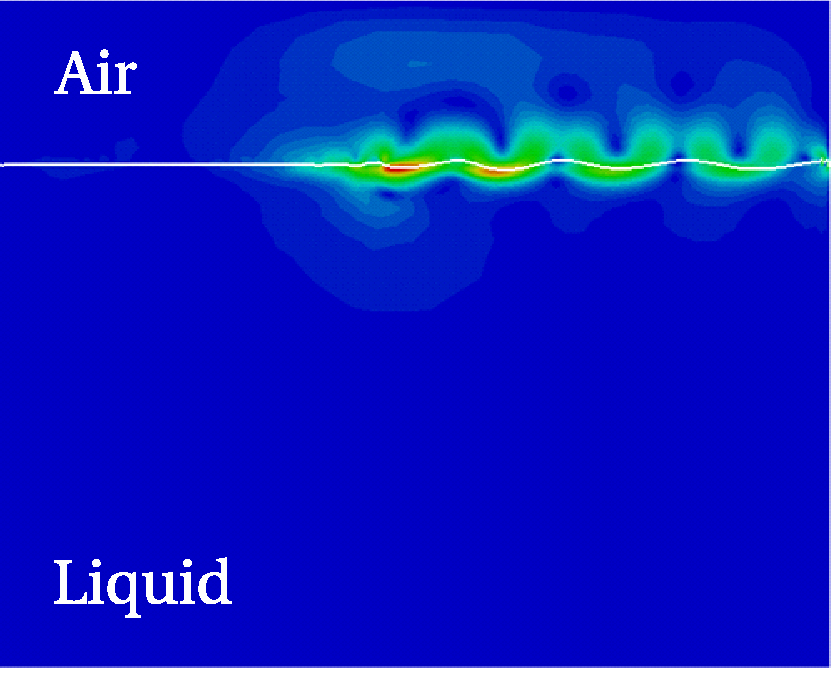
\includegraphics[width=\textwidth]{Chapter5/Graphics/UnstableInterface1.pdf}
% 	\caption{At a certain time increment (without mesh)}
%     \label{fig:UnstableInterface1}
%   \end{subfigure}
% \qquad
%  \begin{subfigure}[t]{0.4\textwidth}
%     \centering
% 	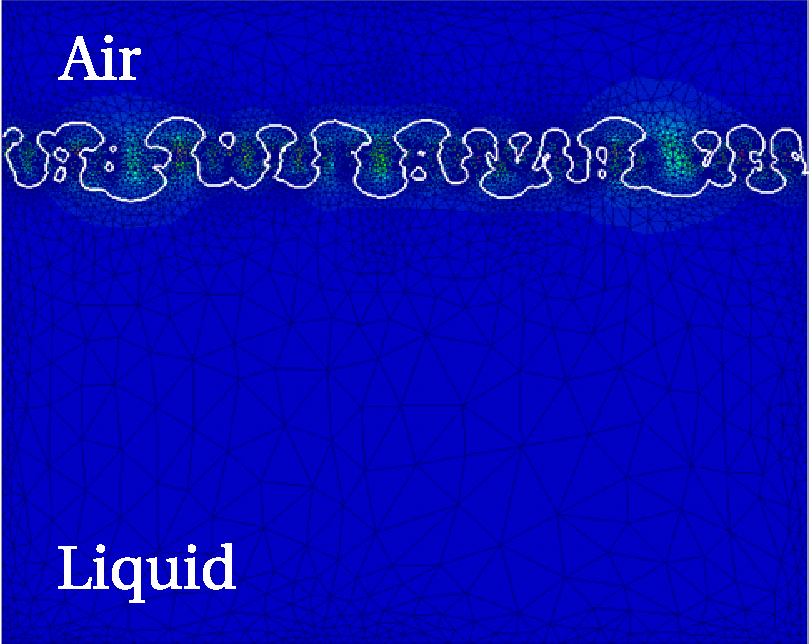
\includegraphics[width=\textwidth]{Chapter5/Graphics/UnstableInterface2.pdf}
% 	\caption{Another time increment (with mesh)}
%     \label{fig:UnstableInterface2}
%   \end{subfigure}
% \caption{Interface destabilisation under the effect of high properties ratio across the interface.}
% \end{figure}
% %----------------------
% %%---------

% \subsubsection{Modified coupling}
% In contrast to a classic coupling, here we attempt to modify the velocity field before feeding to the transport solver.
% The main motivation for considering this approach is the lack of stability that we observed whenever the mechanical
% properties of the fluids were different by several orders of magnitude.
% The algorithm should simultaneously fulfil these requirements: 
% \begin{itemize}
% \itemsep0em
% \item support high ratios of fluids density with close viscosities by preserving an non-oscillating interface,
% \item maintain a horizontal level at the free surface of the melt,
% \item follow shrinking metal surface profile in solidfying regions,
% \item satisfy the mass conservation principle, essentially in the metal.
% \end{itemize}
% We want to process the original transport velocity by imposing a uniform motion (speed and direction) 
% at the nodes of the free surface, and at the same time, be able to follow the pipe formation at the 
% surface as a result of solidification shrinkage, as shown in \cref{fig:horizontal_liquid_surface}.

% %----------------------
% \begin{figureth}
% % textwidth 
% {0.8}
% %path 
% {Chapter5/Graphics/FreeSurface.pdf}
% % caption
% {Snapshot of a solidifying ingot by a cooling flux from the side. The profile of the actual surface changes in solid and mushy regions
% to adapt the new density while staying perfectly horizontal in the liquid phase.}
% % label
% \label{fig:horizontal_liquid_surface}
% \end{figureth}
% %-----------------------------------
% %
% \comment{How to transport level set using velocity from momentum conservation DIRECTLY or AVERAGED PER ELEMENTS, 
% show examples of instability/stability when using false/nominal air properties \\ 
% Validation of LS transport: perform test case simulation of buoyancy driven air droplet in water by 2005Nagrath that I also have seen 
% in Shyamprasad's masters report). => I didnt notice: what time step $\delta t$ did they use ? }
% %
% %----------------------
% \begin{figureth}
% % textwidth 
% {0.8}
% %path 
% {Chapter5/Graphics/AvgTransport/BottomSideCooling.pdf}
% % caption
% {Treatment of liquid free surface in a) bottom and b) side heat extraction configurations. The dashed line represents the 
% initial level of the free liquid surface.}
% % label
% \label{fig:bottom_side_cooling}
% \end{figureth}
% %-----------------------------------

% The general idea is read the velocity around the interface up to a certain thickness, which may be the same 
% thickness as the diffuse interface defined in \cref{sec:heaviside}, then compute a volumetric average
% from all the elements in the thickness. This average is then given to the transport solver, which will apply
% the same magnitude and direction to transport the interface. However, as we only need the transport velocity
% to be uniform within the "100\% liquid" elements, it should not be the case for the other elements that belong 
% either to the mushy zone or the solid region, where shrinkage is taking place.
% Therefore, depending on the heat extraction configuration, two scenarios are possible. If heat extraction is far from
% the interface, i.e. there is not direct contact as in \cref{fig:bottom_side_cooling}a, 
% the surface area remains unchanged at any time, hence all the elements
% around the interface are "100\% liquid". This happens when a bottom cooling is applied to the ingot. In contrast, if a side cooling 
% is applied as shown in \cref{fig:bottom_side_cooling}b, the surface area of the interface will be reduced over time
% as a consequence of the solid front progression. In this case, the average transport velocity should be computed only
% from the elements belonging to the free surface. The remaining part of the interface which belongs to partial or full 
% solid regions, is transported with Navier-Stokes output, which should be some orders of magnitude less than the velocity
% imposed at the free surface, as a result of a decreasing permeability.

\cleardoublepage
%--------------------------------
%--
\section{1D application: solidification with inverse segregation}
%--------------------------------------------
\subsection{Geometry and boundary conditions}
A simple but very efficient way of analysing the model is to test it through a 1D flow configuration with energy and species conservation.
For this purpose, we take an aluminium-silicon alloy with the properties shown in \cref{table:data_case_inverseseg}.

%------------------------
\begin{tabulate}
% caption 
{Parameters for the 1D inverse segregation test case with a binary \bin{Al}{7}{Si} alloy.}
% label
{table:data_case_inverseseg}
% line separation (e.g. 1.5mm)
{1.0mm}
% column justification-number (e.g. |c|ll|)
{llll}
% header titles (should use the & sign to switch columns)
%------------------------------------------------------------------------------------------
{\textbf{Parameter} & \textbf{Symbol} & \textbf{Value} & \textbf{Unit}}
% cells content (should use the & and // to switch columns and rows)
%------------------------------------------------------------------------------------------
{Nominal composition 				& $w_0$ 			& \num{7} 		& \si{\ucomposition} \\ 
% Liquidus temperature 				& $T_L$ 			& \num{618} 	& \si{\udegC} \\ 
% Eutectic temperature 				& $T_E$ 			& \num{577}	 	& \si{\udegC} \\  
% Segregation coefficient 			& $k$ 				& \num{0.13} 	& $-$  \\  
% Liquidus slope 						& $m_L$ 			& \num{-6.5} 	& \si{\uslope} \\ 
Liquid density			 			& $\rhol$ 			& \num{2600} 	& \si{\udensity} \\  
Solid density	 					& $\rhos$ 			& \num{2800} 	& \si{\udensity} \\  
Air density 						& $\rhoa$ 			& \num{1.3} 	& \si{\udensity} \\  
Liquid viscosity			 		& $\mul$ 			& \num{d-3} 	& \si{\uviscosity} \\  
Solid viscosity	 					& $\mus$ 			& (Darcy) 			& \si{\uviscosity} \\  
Air viscosity 						& $\mua$ 			& \num{d-4} 	& \si{\uviscosity} \\  
Liquid heat capacity 		 		& $C_p^l$ 			& \num{1000} 	& \si{\umasscapacity} \\  
Solid heat capacity 		 		& $C_p^s$ 			& \num{928.57} 	& \si{\umasscapacity} \\  
Air heat capacity 		 			& $C_p^a$ 			& \num{1000} 	& \si{\umasscapacity} \\  
Enthalpy of fusion 				 	& $L$ 				& \num{365384} 	& \si{\umassenergy} \\ 
Thermal conductivity 				& $\kappa$ 			& \num{70} 		& \si{\uconductivity}	\\
Solute diffusion in the liquid		& $\Dl$ 			& \num{1e-9} 	& \si{\udiffusivity} \\  
Solute diffusion in the solid		& $\Ds$ 			& \num{0} 	& \si{\udiffusivity} \\  
Solute diffusion in the air	(fictitious)	& $\Da$ 	& (varies with case) 	& \si{\udiffusivity} \\  
\hline  %------------------------------------------------------------------------------------------
Heat transfer coefficient 			& $\hext$ 			& \num{500} 	& \si{\uhconvec} \\ 
External temperature 				& $\Text$ 			& \num{100} 	& \si{\udegC} \\ 
Initial temperature 				& $T_0$ 			& \num{800} 	& \si{\udegC} \\ 
Ingot length 						&  					& \num{0.1} 	& \si{\metre} \\ 
\hline %------------------------------------------------------------------------------------------
FE mesh size 						&  					& \num{e-3} 	& \si{\metre} \\ 
Time step 							& $\dt$ 			& \num{0.1} 	& \si{\second} \\ 
Convergence criterion (residual) 	& $\varepsilon_R$	& \num{e-6} 	& $-$ \\ 
Convergence criterion (temperature) & $\varepsilon_T$ 	& \num{e-2} 	& \si{\udegK}}
%--------------------------------------------------------------------------------------------------
\end{tabulate}
%------------------------

The major difference with respect to the former validation setup is the air domain that should also be included in the mesh.
We consider a 2D domain having as dimensions \SI{0.14}{\metre}$\times$\SI{0.001}{m}, where initially the air column's height is only \SI{0.04}{\metre}
and the remainder of the length is for the metal.  
\Cref{fig:1d_alsi7_geobc} shows the geometry and boundary conditions used for the simulations in this section. In the same figure, the thermal and mechanical boundary conditions are shown.
In the latter, velocity-slip conditions were imposed on the lateral boundaries while a no-slip was used at the bottom where heat is extracted,
and a free-velocity condition is set at the top of the domain, to ensure a 1D air flow from the top air inlet. 

In this case, imposing slip conditions on lateral sides is two-fold: on one hand, we need to ensure that the fluid flow solution
remains one-dimensional, hence symmetry on the boundaries solves the issue, while on the other hand during solidification, 
the resulting feeding flow should be able to transport the interface intersecting with boundary nodes. If boundary velocities
are zero, then the interface transport will face problems at these boundary nodes. This is indeed an important and relevant point 
in the next 2D test case.

%--------------
\begin{figureth}
% textwidth 
{1.0}
%path 
{Chapter5/Graphics/1d/geobc.pdf}
% caption
{Computational configuration for the 1D inverse segregation case showing the domain geometry with the applied boundary conditions to it.}
% label
\label{fig:1d_alsi7_geobc}
\end{figureth}
%--------------

%
\subsection{Shrinkage without macrosegregation}
%----------------------------------------------------

The first simulation is for solidification without any segregation, hence a unique solidification path is considered at $\Cnominal=$\SI{7}{\ucomposition},
shown in \cref{fig:shrinkage_nomacro_sp}.
This case is interesting as a reference case, where we can study volume shrinkage and level set behaviour in a simple segregation-free configuration.
We first use a homogeneous isotropic mesh of constant size $h=$ \SI{200}{\micro \metre}. The liquid and solid phase densities are assumed constant
and respectively equal to \SI{2600}{\udensity} and \SI{2800}{\udensity}. This density difference is equivalent to a ratio of $\beta_{SS}= \brac{\rhos-\rhol}/\rhos$,
also termed as \emph{solidification shrinkage} by \citet{flemings_macrosegregation:_1967}. 
In the current conditions, $\beta_{SS}$ is constant and equal to \SI{7.14}{\percent}. 
The domain is initially meshed before any resolution, as shown in \cref{fig:1dalsi7_lsmixing}, in a way to reduce interpolation errors that may
cause coarse elements within the transition of fluids density and dynamic viscosity, reminding that these parameters are crucial for the stability 
of the velocity solution used later in the transport step. The chosen mixing laws are arithmetic for the density and logarithmic for the viscosity.
The choice is based on tests done in former Ph.D. projects at CEMEF. 
The mesh properties are given in \cref{table:1dalsi7_meshsize}.

%--------------------------------
\begin{table}[htbp]
\centering
\caption{Summary of the different mesh sizes used to generate an adaptive anisotropic mesh, along with the level set mixing thickness, $\varepsilon$. 
Refer to \cref{sec:remesh2_params} for the definition of each mesh parameter.}
\label{table:1dalsi7_meshsize}
{\tabulinesep=1.0mm \begin{tabu}{ll}
\tabucline[1pt]{-}
\textbf{Mesh parameter} & \textbf{Size [\si{\metre}]} \\\tabucline[1pt]{-}
%-----------------------------
$\varepsilon $			&	\num{2.5e-4}	\\
$h_{\vec{n}}$ 			&	\num{2.5e-5}	\\ 
$h_{\vec{\tau}}$ 		&	\num{2e-4}		\\ 
$h_M$  					&	\num{1.5e-4}	\\
$h_A$  					&	\num{2.5e-4} 	\\
Number of nodes 		&   $\approx$\num{7e3} \\ 
Number of elements 		&   $\approx$\num{1e4} \\\tabucline[1pt]{-}
%-----------------------------
\end{tabu}}
\end{table}
%--------------------------------

%--------------
\begin{figureth}
% textwidth 
{1.0}
%path 
{Chapter5/Graphics/1d/ls_mixing.pdf}
% caption
{Snapshots of (a,b) the initial adapted mesh around the interface with different mesh sizes in the air and the metal. The adapted region
is stretched beyond the level set mixing thickness to ensure better interpolation around the interface, in case of emergence of diffusion
instabilities. To the right, (c)  the reference fluid density and (d) viscosity are plotted in the transition zone. 
% showing a symmetric mixing for the former
% and a shifted mixing for the latter, as a consequence of the mixing laws.
The thick blue line represents the zero isovalue of the distance function.}
% label
\label{fig:1dalsi7_lsmixing}
\end{figureth}
%--------------

%--------------------------------------
\begin{figure}[htbp]
\centering
\begin{tikzpicture}
 \pgfkeys{%
    /pgf/number format/set thousands separator = {}}
\begin{axis}
[
	table/col sep=comma,
	smooth, %ybar
	%stack plots=y,
	%area style,
	enlarge x limits=false,
	legend pos=north west,
	scaled ticks=true,
	xlabel=Temperature (\si{\udegC}),
	ylabel=Volume fraction (-),
	xticklabel style={/pgf/number format/fixed},
	xtick={577, 600, 618},
	%x tick label style={rotate=45,anchor=east},
	%width=0.5\textwidth,
	mark repeat	= {1},
	cycle list name=mycycle, %exotic,
]
\addplot table [x=Temperature, y expr=\thisrow{LIQ}] {Chapter5/Data/1d_alsi7_nominalSP/sp.csv};% \closedcycle ;
\addplot table [x=Temperature, y expr=\thisrow{ALPHA}] {Chapter5/Data/1d_alsi7_nominalSP/sp.csv};%\closedcycle;
\addplot table [x=Temperature, y expr=\thisrow{BETA}] {Chapter5/Data/1d_alsi7_nominalSP/sp.csv};%\closedcycle;

\legend{Liquid, FCC, EUT}
\end{axis}
\end{tikzpicture}

\caption{Unique solidification path at nominal composition for the shrinkage case without macrosegregation in \bin{Al}{7}{Si}.}
\label{fig:shrinkage_nomacro_sp}
\end{figure}
%--------------------------------------

At a first glance, results show that the interface stability is compromised by a chosen time step for a given mesh size, and that the interface dynamics
requires attention even before investigating the feeding flow created by solidification. As a demonstration, \cref{fig:1dalsi7_velocity_dt} shows the effect of different
time steps with the same adaptive meshing parameters. For time steps greater than 0.01 s, Navier-Stokes computations did not converge resulting in a high artificial 
flow quickly destabilising the interface. It should be noted that the frame corresponding to 0.02 s was taken at an earlier time than the two other frames.

%--------------
\begin{figureth}
% textwidth 
{0.6}
%path 
{Chapter5/Graphics/1d/ls_velocity_dt.pdf}
% caption
{Three average fluid velocity frames at different time steps: 0.005 s, 0.01 s and 0.02 s. The first and second frame are taken after 
50 seconds of cooling while for the last frame, the frame was taken after only 1 second of cooling, thus it is crossed to show non-convergence.
The thick black line represents the zero isovalue of the distance function. Properties are given in \cref{table:1dalsi7_comparative_nomacro,table:data_case_inverseseg}
under case ``R''.}
% label
\label{fig:1dalsi7_velocity_dt}
\end{figureth}
%--------------

Although no solidification has yet started at 100 s, a two-dimensional flow is observed around the interface, while tends to \SI{e-8}{\uvelocity} elsewhere in the ingot.
\Cref{fig:1dalsi7_velocity_dt} confirms that this flow is still predicted at smaller time steps. This flow seems like a pure numerical response
to the properties jump across the interface, namely density and dynamic viscosity. It is also noted that the interface position
is not modified by the neighbouring currents, that reach a maximum magnitude of \SI{e-4}{\uvelocity}. Therefore, the optimal time step for this simulation is set to 0.01 s, and we refer to it as case R, which stands for "real" air.

The fact that properties transition is crucial in the solution stability, is investigated by 2 reference cases, having equal properties 
(density and dynamic viscosity) but with different time steps, 0.01 (case A1) and 0.1 s (case A2), where "A" stands for artificial.
All simulation cases are grouped in \cref{table:1dalsi7_comparative_nomacro}.

%--------------------------------
\begin{table}[htbp]
\centering
\caption{Summary of the comparative shrinkage simulations without macrosegregation.}
\label{table:1dalsi7_comparative_nomacro}
{\tabulinesep=1.0mm \begin{tabu}{llll}
\tabucline[1pt]{-}
\textbf{Case} & \textbf{Air viscosity [\si{\uviscosity}]} & \textbf{Air density [\si{\udensity}]} & \textbf{Time step [s]} \\\tabucline[1pt]{-}
%-----------------------------
R			& \num{e-4}	&	\num{1.3}	&	0.01	\\
A1			& \num{e-3}	&	\num{2600}	&	0.01	\\
A2			& \num{e-3}	&	\num{2600}	&	0.1		\\\tabucline[1pt]{-}
%-----------------------------
\end{tabu}}
\end{table}
%--------------------------------

When the air domain is given the metal's properties, it becomes denser and more viscous by several orders of magnitude. 
\Cref{fig:1dalsi7_caseA1A2}, in which cases A1 and A2 are compared, shows no noticeable sign of velocity instability near the interface before 200 s.
It can be explained by the fact that the air behaves mechanically like a fluid metal given similar properties, 
therefore no steep transitions are computed at the interface. 
However, it is interesting to compare results of \cref{fig:1dalsi7_equalprops_smallstep1} and \cref{fig:1dalsi7_equalprops} at 600 s.
For case A1, the interface is slightly skewed due to slower flow at the left side of the interface, while for case A2, the flow disturbs
the interface deforming it until the end of solidification, as seen at 1000 s. This shows the importance of the chosen time step
in the Navier-Stokes solver. 
% A common issue for all three case, A1, A2 and R, approximately at 400 s (not visible in the figures), is the the mushy zone enters within the diffuse interface, 
% affecting the level set transport and thus causing mass conservation problems. These problems are discussed in the next section.

In contrast, \cref{fig:1dalsi7_differentprops} shows more viable results as far as the level set transport is concerned.
From 200 s to 800 s, the local flow instability (discussed earlier in \cref{fig:1dalsi7_velocity_dt}) is sustained, even until after solidification is complete.
However, in regions of 100\% metal and 100\% air the computed velocity is nearly the same order of magnitude as predicted for all three simulations.
Finally, in \cref{fig:1dalsi7_differentprops}, we notice a recirculating air flow in the vicinity of the interface as no metal shrinkage 
may further occur once solidification is complete, thus air flows freely in and out 
of the upper boundary with a very low magnitude ($\sim$ \SI{e-7}{\uvelocity}), while impinging on the metal-air surface.
Regarding the CPU times, cases A1 ran for 14 hours, case A2 took only 2 hours while case R ran for 23.3 hours.
To summarise, we can see conclude from the previous results, the following points:
\begin{enumerate}
	\itemsep0em 
	\item Greater differences in mechanical properties of fluids across the level set impose using smaller time steps,
	\item When real properties are used, smaller time steps are needed to capture the variations across the moving level set, hence inducing longer simulation time,
	\item In a situation where the flow dynamics in the non-metallic (gas) domain is not a primary objective, one can 
		   use artificial properties instead of the real values, hence gaining in computation time at the expense of the flow prediction accuracy.
\end{enumerate}  
%-----------------------------------------
\begin{figure}[htbp]
\centering
%======
  \begin{subfigure}{0.55\textwidth}
  \centering
    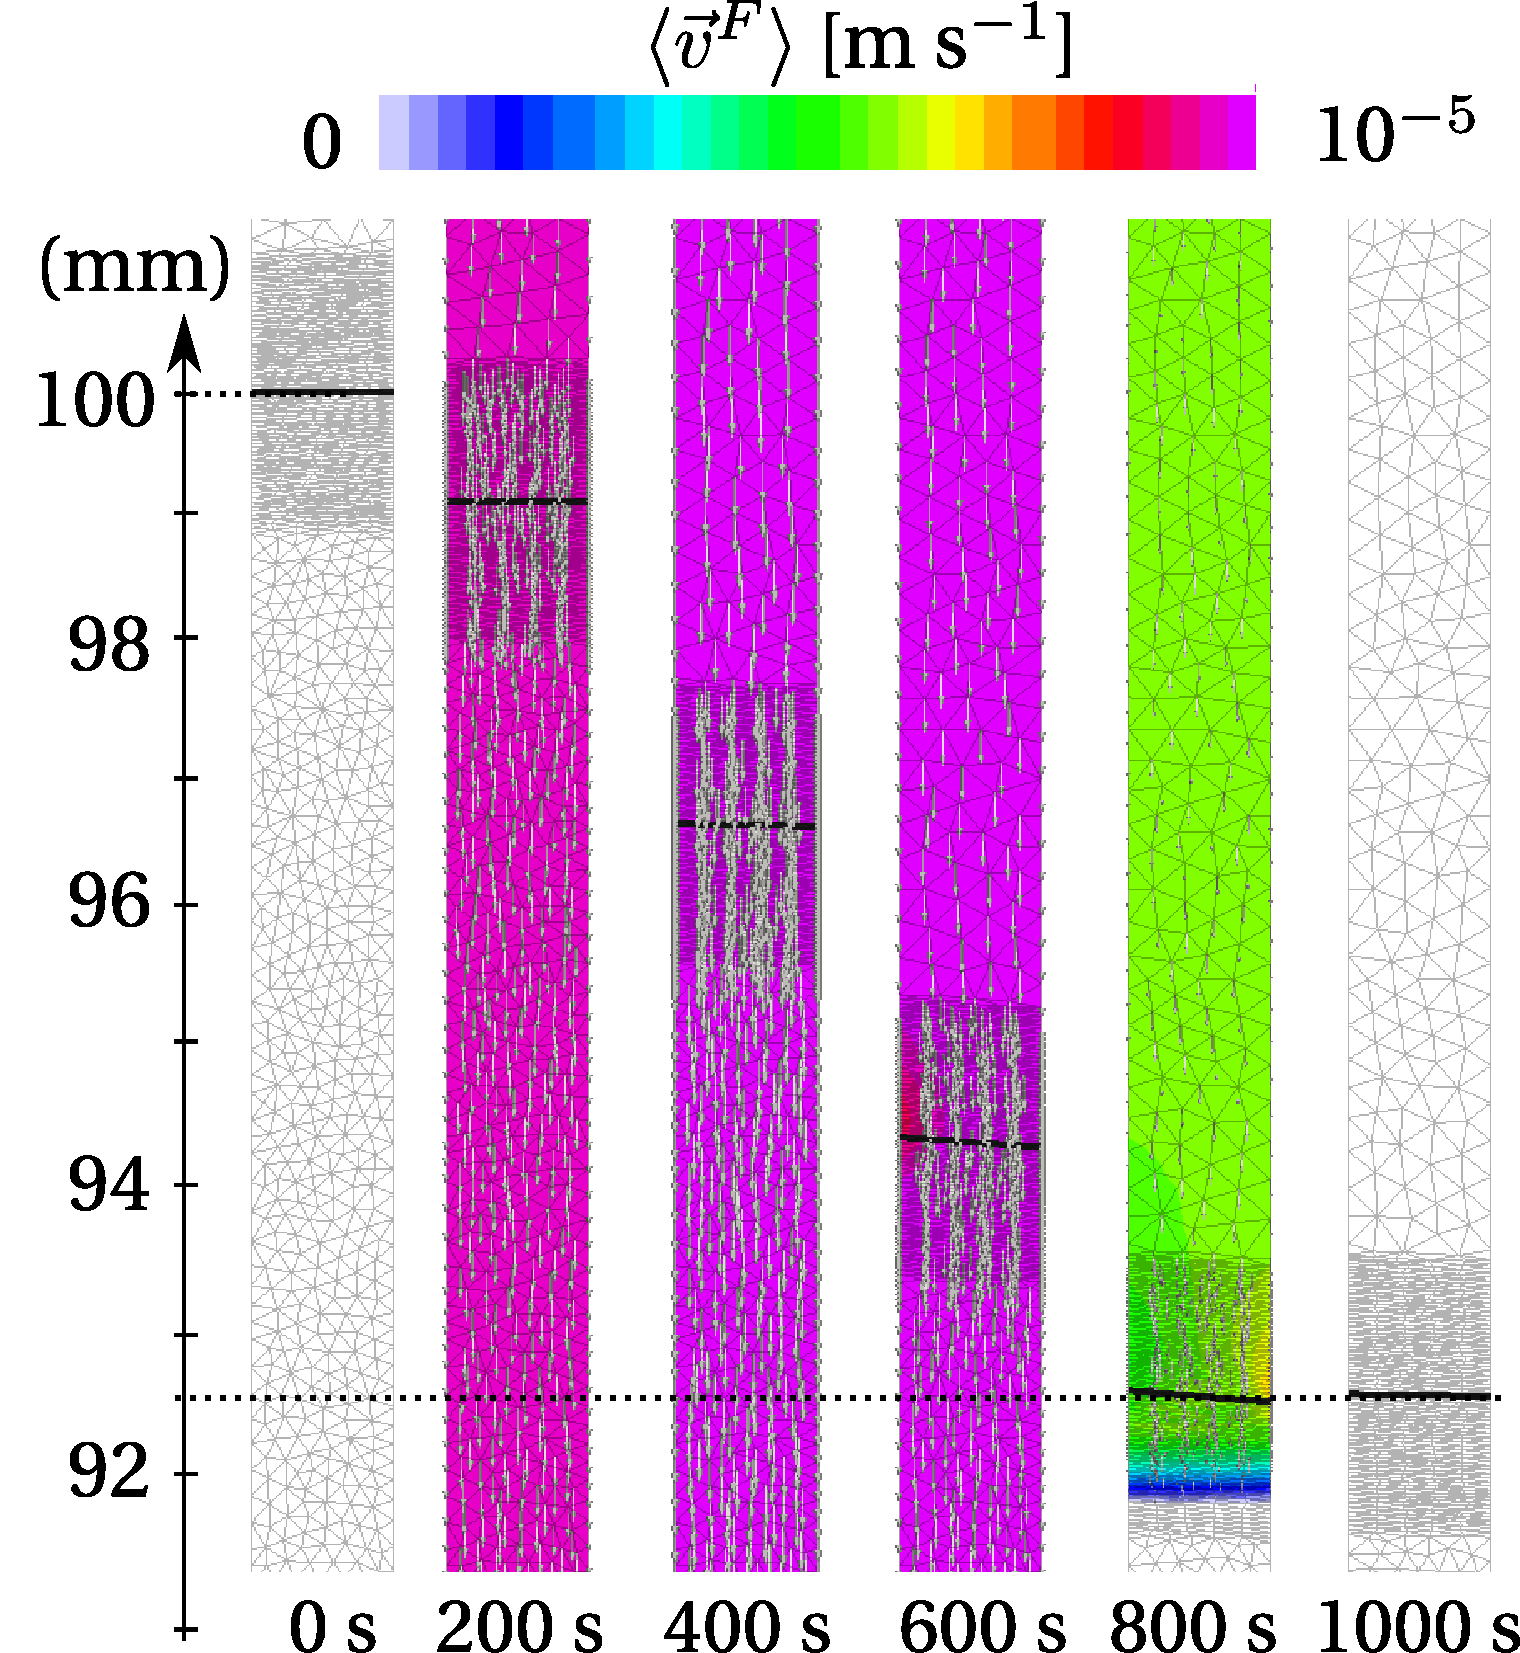
\includegraphics[width=\textwidth]{Chapter5/Graphics/1d/ls_velocity_equalprops_1e-2.pdf}
	\caption{Case A1}
    \label{fig:1dalsi7_equalprops_smallstep1}
  \end{subfigure}  
%======
\vskip\baselineskip
%======
  \begin{subfigure}{0.55\textwidth}
    \centering
    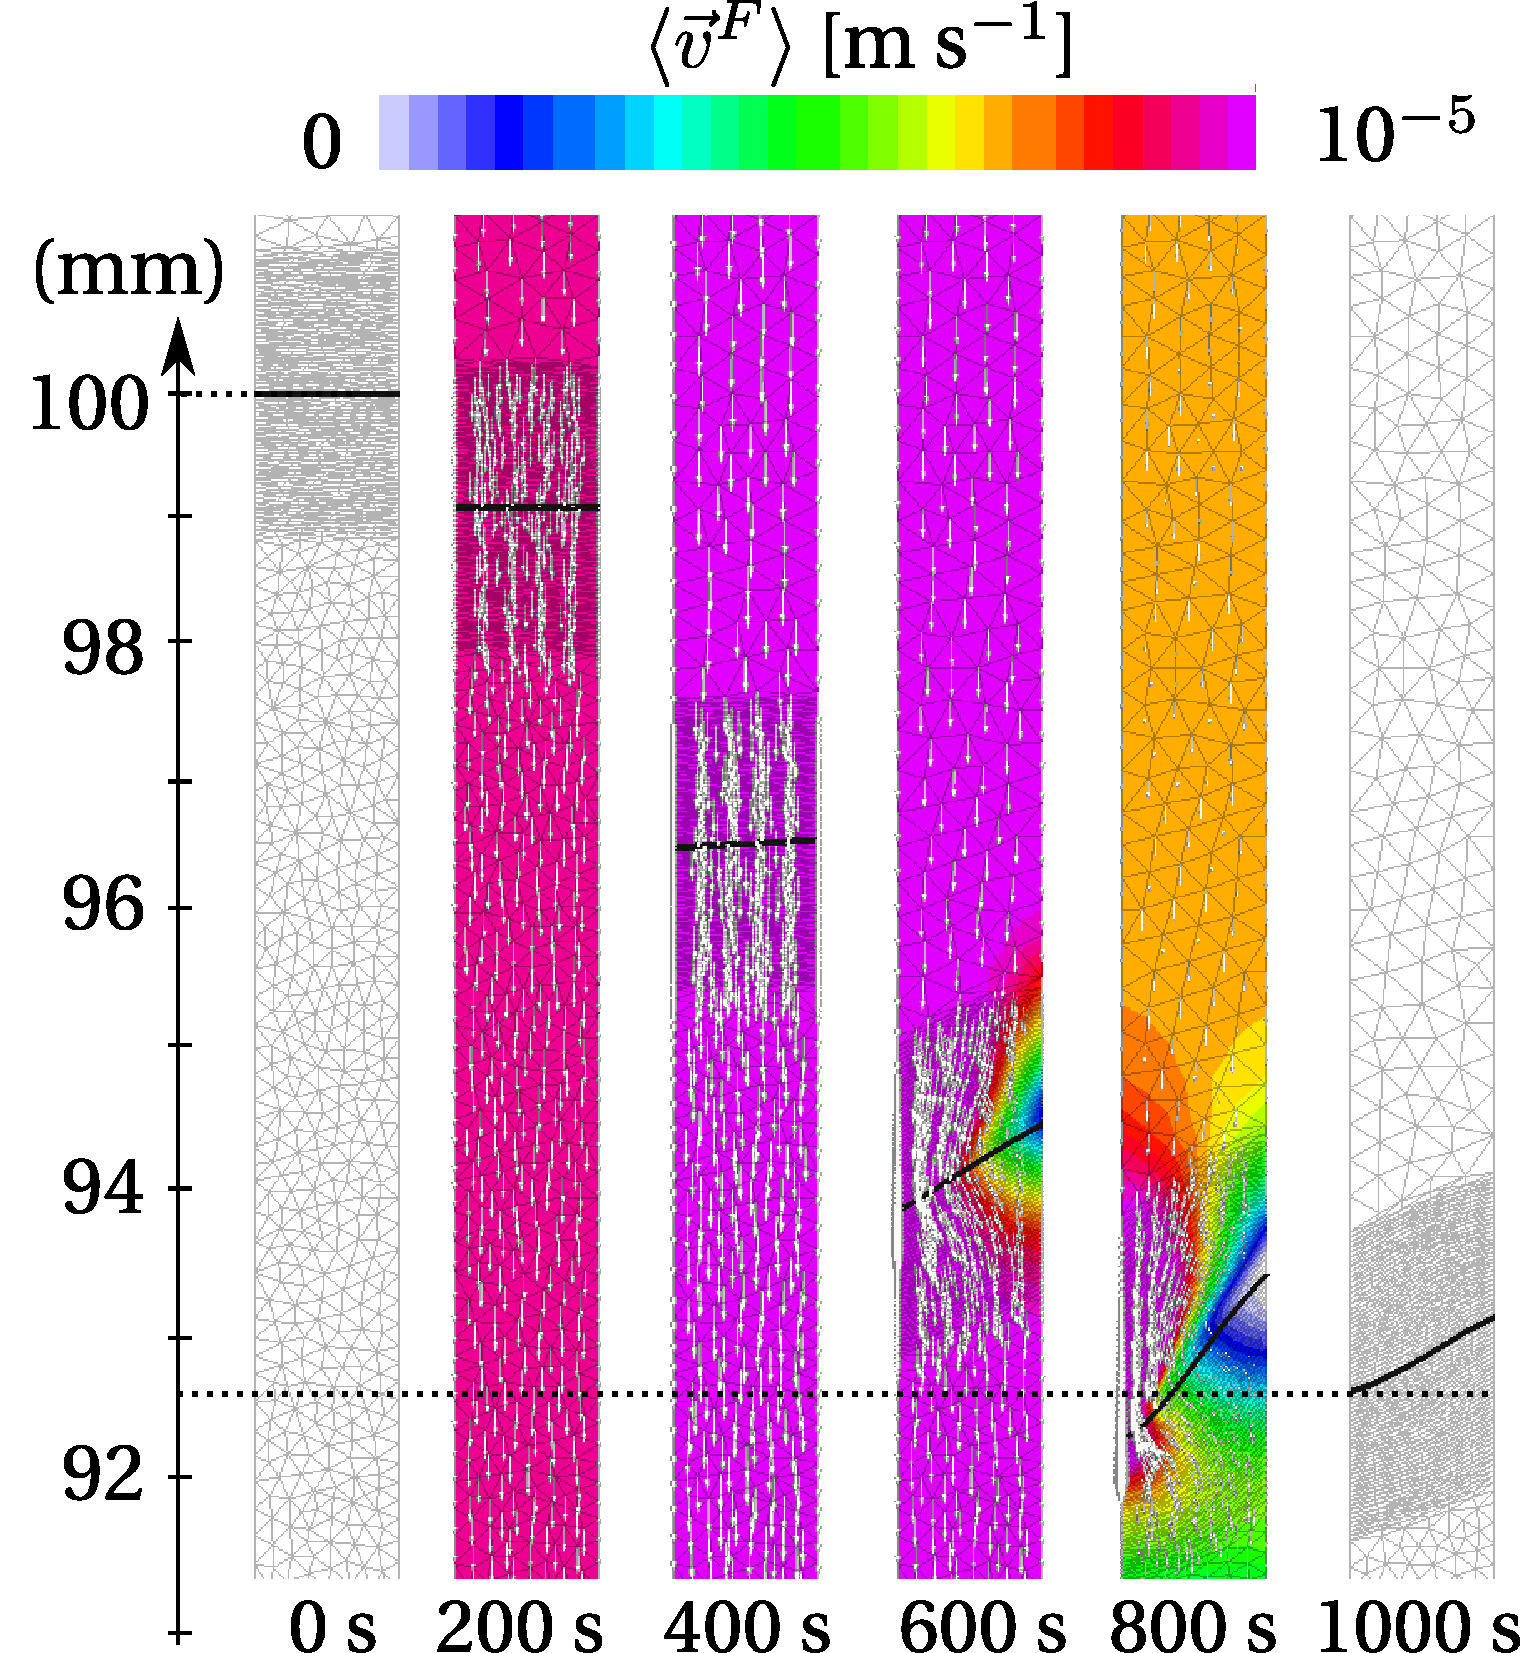
\includegraphics[width=\textwidth]{Chapter5/Graphics/1d/ls_velocity_equalprops.pdf}
	\caption{Case A2}
    \label{fig:1dalsi7_equalprops}
  \end{subfigure}
%======
\caption{Comparison of two simulations at several stages of solidification ending shortly after 800 s.
The results shows the influence of density and viscosity properties across the level set interface.
The plotted field is the average fluid velocity, on which the corresponding nodal vectors are superimposed, mainly pointing
downwards, i.e. towards the solidification front. The thick black line represents the zero isovalue of the distance function.
Properties are given in \cref{table:data_case_inverseseg,table:1dalsi7_meshsize,table:1dalsi7_comparative_nomacro}.}
\label{fig:1dalsi7_caseA1A2}
\end{figure}
%-----------------------------------------

%-----------------------------------------
\begin{figure}[htbp]
\centering
%======
  \begin{subfigure}{0.55\textwidth}
  \centering
    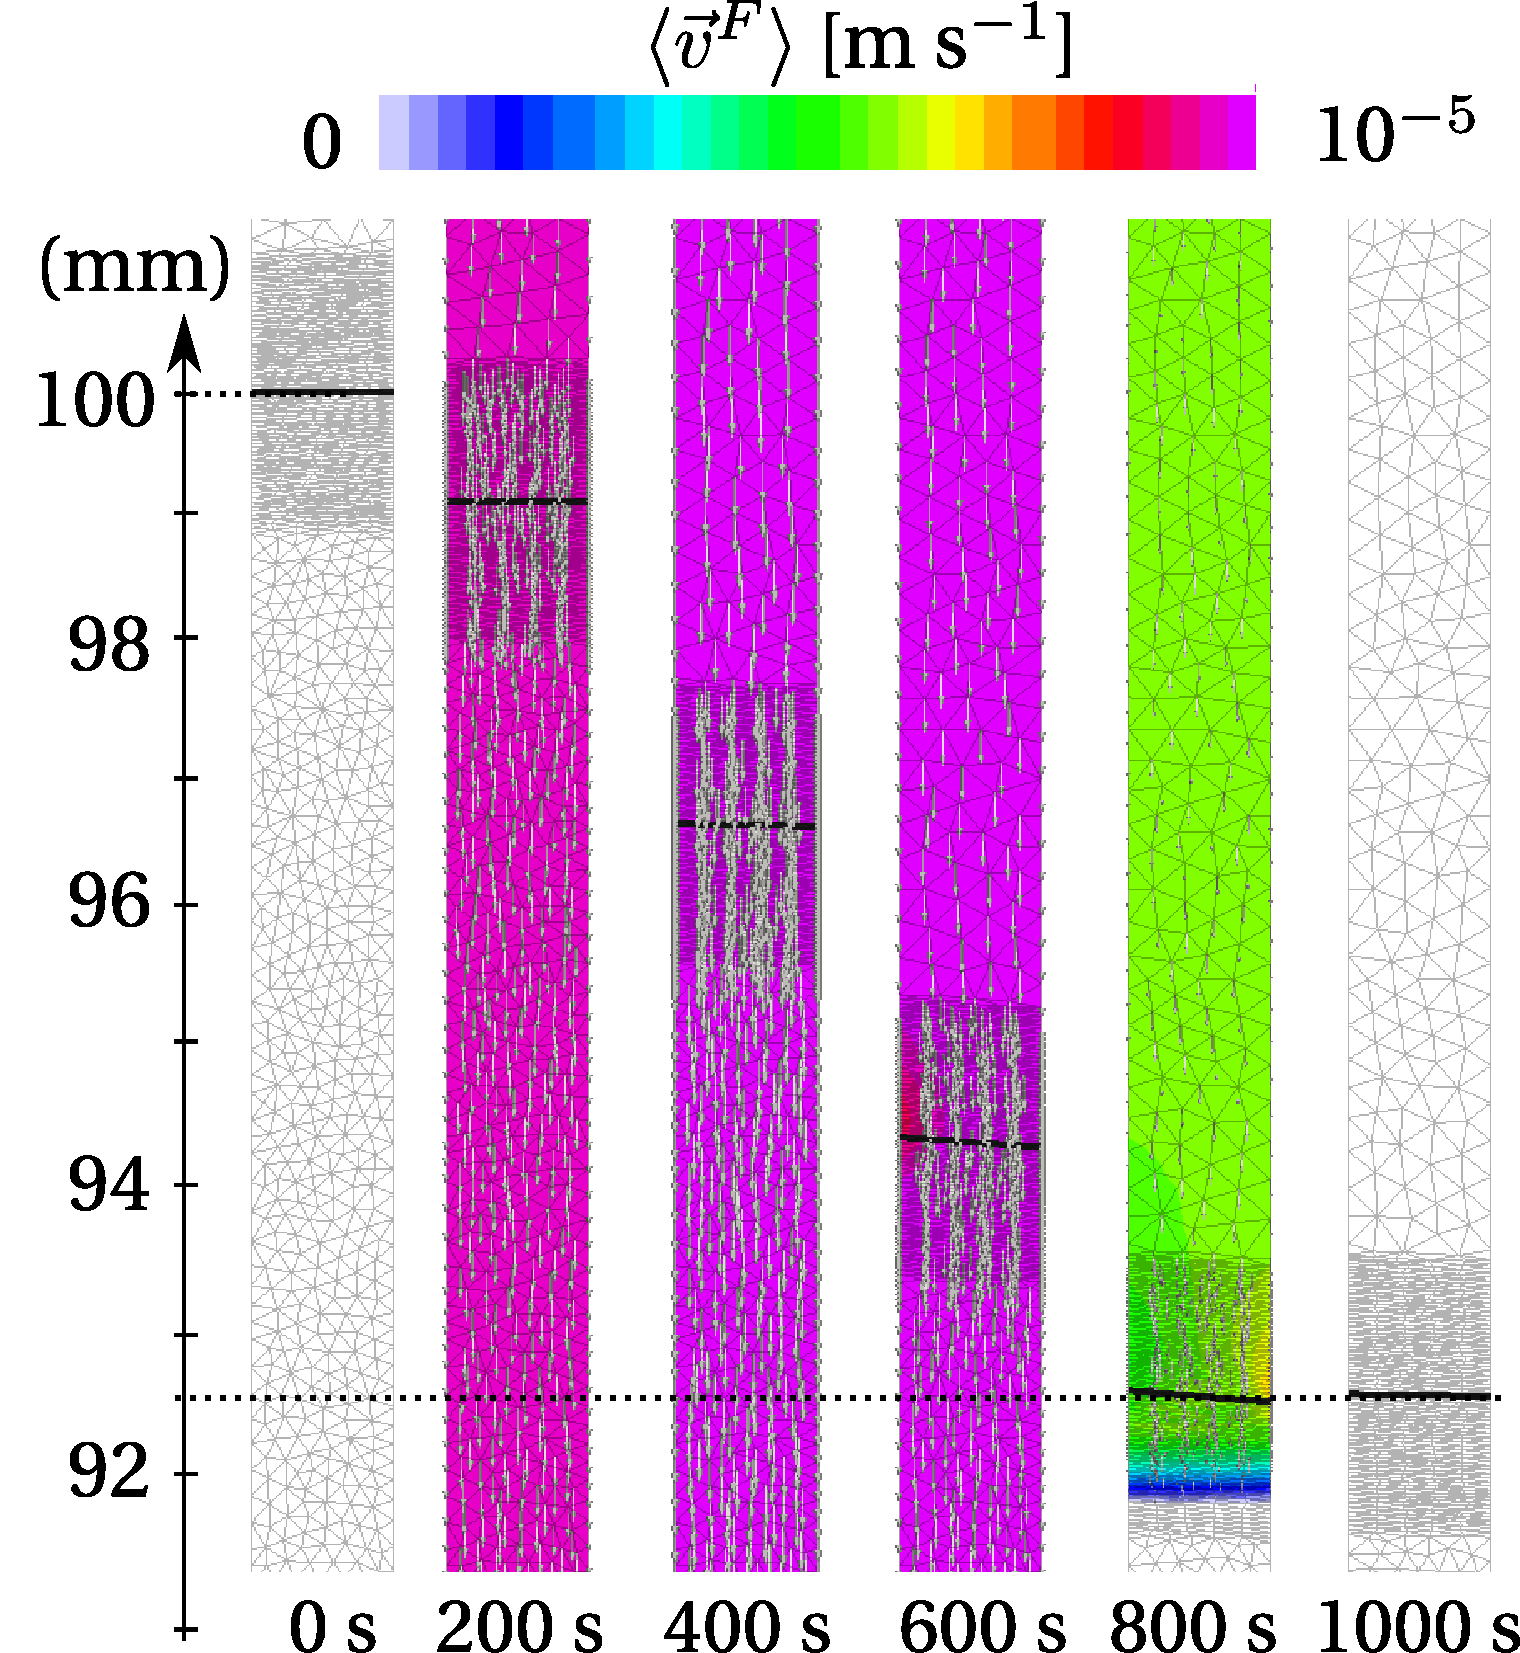
\includegraphics[width=\textwidth]{Chapter5/Graphics/1d/ls_velocity_equalprops_1e-2.pdf}
	\caption{Case A1}
    \label{fig:1dalsi7_equalprops_smallstep2}
  \end{subfigure}  
%======
\vskip\baselineskip
%======
  \begin{subfigure}{0.55\textwidth}
    \centering
    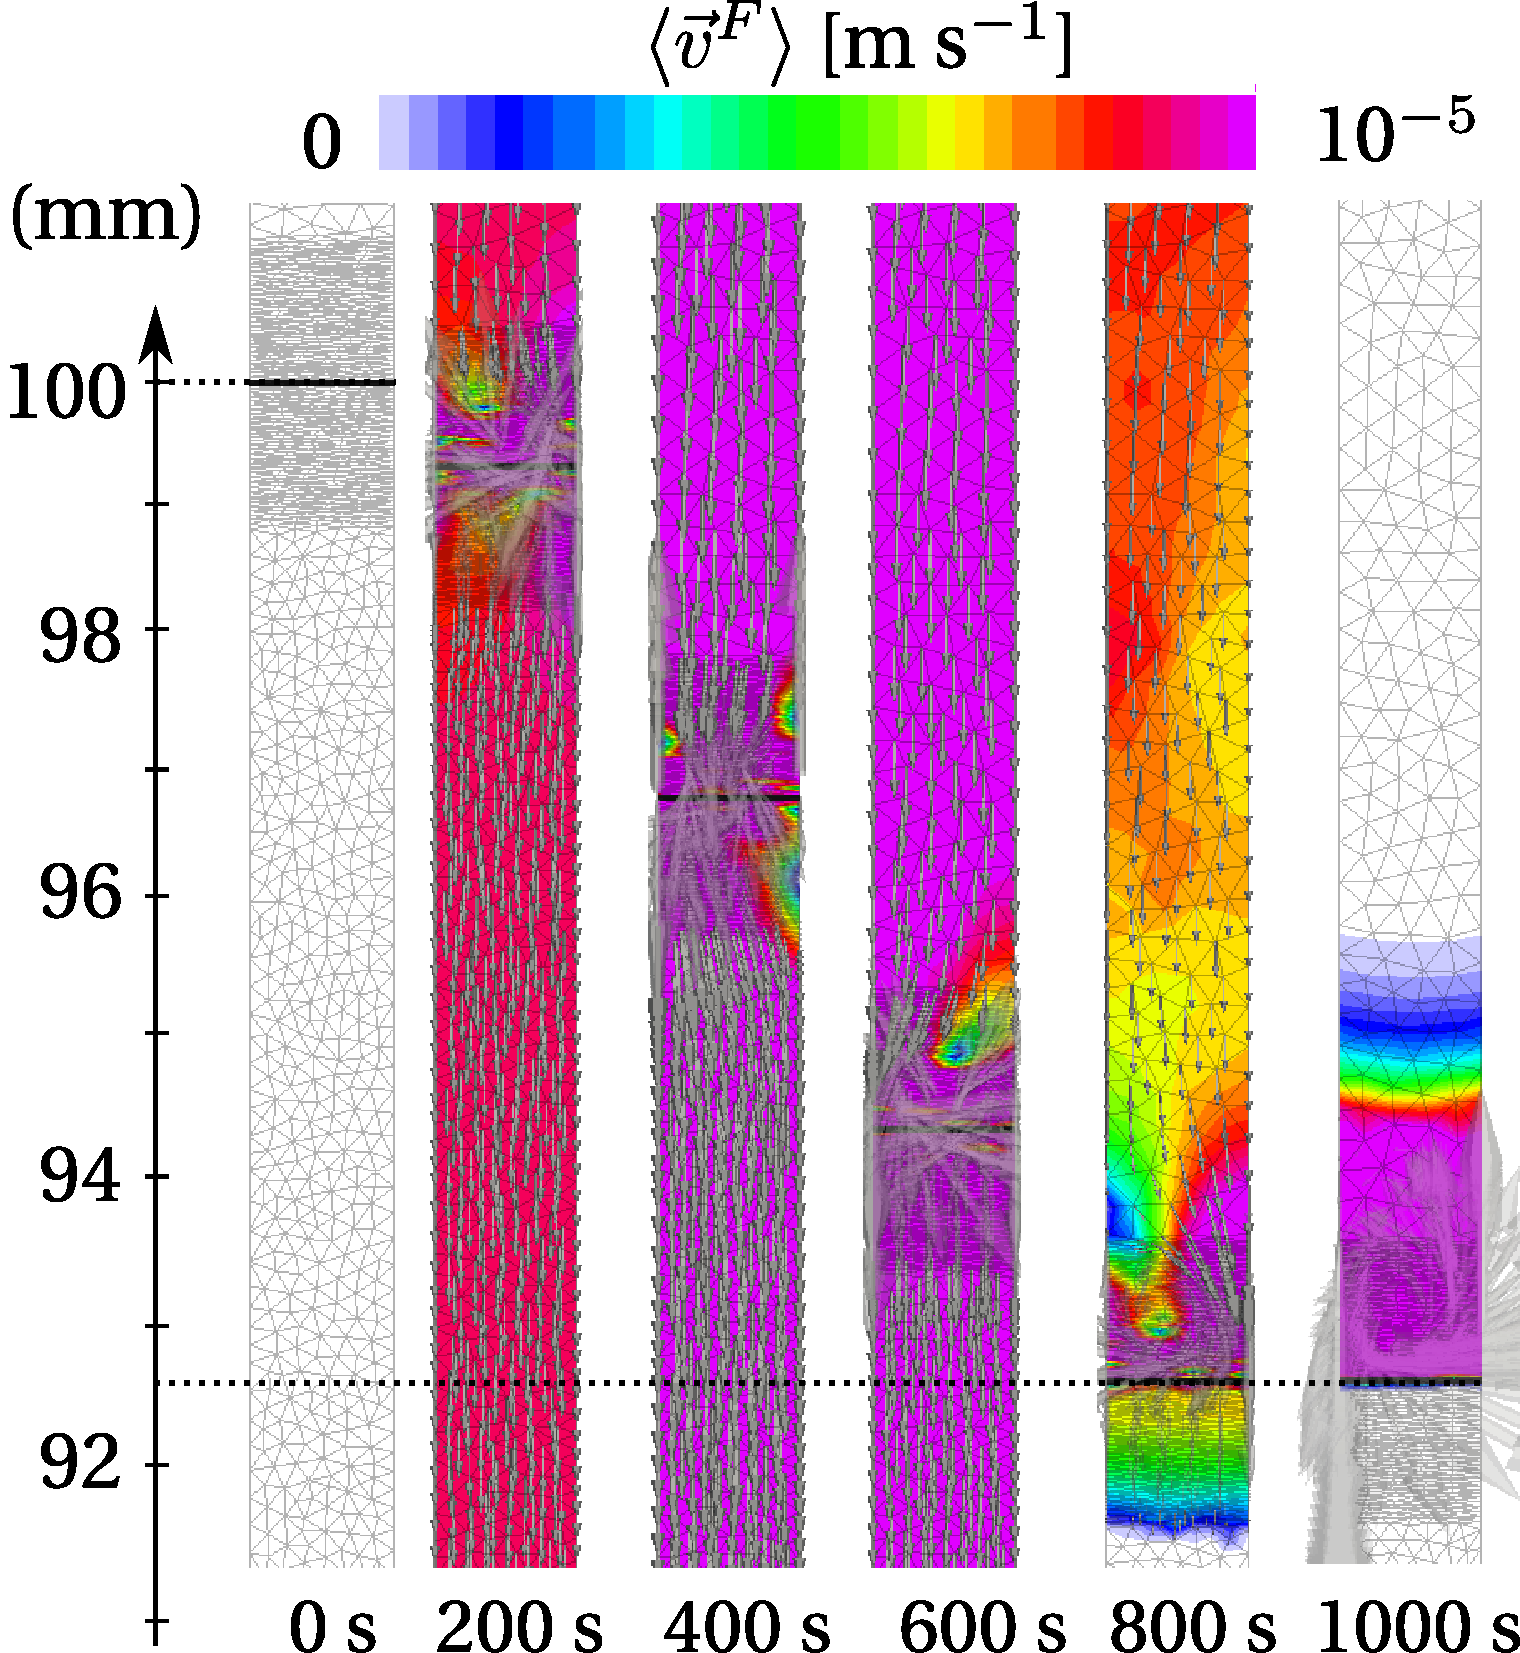
\includegraphics[width=\textwidth]{Chapter5/Graphics/1d/ls_velocity_differentprops.pdf}
	\caption{Case R}
    \label{fig:1dalsi7_differentprops}
  \end{subfigure}
%======
\caption{Comparison of two simulations at several stages of solidification ending shortly after 800 s.
The results shows the influence of density and viscosity properties across the level set interface.
The plotted field is the average fluid velocity, on which the corresponding nodal vectors are superimposed, pointing
towards the solidification front.Properties are given in \cref{table:data_case_inverseseg,table:1dalsi7_meshsize,table:1dalsi7_comparative_nomacro}.}
\label{fig:1dalsi7_caseA1R}
\end{figure}
%-----------------------------------------

\subsubsection{Mass conservation study}

In order to get a better idea about the performance of our model, a mass conservation study may be enlightening. 
We define the metal's mass as a function of the 
metal's average density and the Heaviside function relative to the metal domain, as follows:
%----------------
\begin{align}
\label{eq:metal_mass}
& m^M = \integral{\Ohm}{H^M \avg{\rho}^M}{\Ohm}	
\end{align}
%---------------
Then, the mass conservation can be monitored by processing \cref{eq:metal_mass} at each time step, and computing
the relative mass change by writing:
%----------------
\begin{align}
\label{eq:metal_mass_variation}
&  m^M_\% = \frac{m^M - m^M_0}{m^M_0} \times 100	
\end{align}
%---------------
The relative mass change gives us information on the level set transport.
As the current case is 1D and phase densities are constant throughout the simulation, mass conservation can be 
checked in a much simpler approach than by checking \cref{eq:metal_mass_variation}. Since we know the initial metal's column
length, $l^M_0$, and the expected solidification shrinkage is \SI{7.14}{\percent}, we should expect a final length of 
$l^M_f= \brac{1-\beta_{SS}} l^M_0 =$\SI{92.86}{\milli\metre}. 
% However, this equation is very useful and applicable in 2D and 3D
% cases of solidification shrinkage.
%--------------------------------------
\begin{figure}[htbp]
\centering
\begin{tikzpicture}
 \pgfkeys{%
    /pgf/number format/set thousands separator = {}}
%================================================
\begin{axis}
[	name=artificial,
	title=(a) Case A1,
	scale only axis,
	table/col sep=tab,
	enlarge x limits=false,
	legend pos=north west,
	scaled ticks=true,
	xlabel=Time (s),
	ylabel=$m^M_\%$ (\%),
	xticklabel style={/pgf/number format/fixed},
	xtick={0,200,400,600,800,1000},
	ytick={-0.1,0,0.1,0.2},
	%x tick label style={rotate=45,anchor=east},
	width=0.4\textwidth,
	%height=5cm,	
	ymin=-0.1, ymax=0.2,
	mark repeat	= {30},
	cycle list name=mycycle, %exotic,
]
\addplot table [x=Temps, y=mMpct] {Chapter5/Data/1d_alsi7_mass/ArtificialDarcyBlocking0pct_smallstep.txt}; %\closedcycle; 
%\addplot table [x=Temps, y=mMpct] {Chapter5/Data/1d_alsi7_mass/ArtificialDarcyBlocking25pct.txt}\closedcycle;
%\addplot table [x=Temps, y=mMpct] {Chapter5/Data/1d_alsi7_mass/ArtificialDarcyBlocking50pct.txt}\closedcycle;
%\addplot table [x=Temps, y=mMpct] {Chapter5/Data/1d_alsi7_mass/ArtificialDarcyBlocking99pct.txt}\closedcycle;
%\legend{Blocking at 0\% $\gl$, Blocking at 25\% $\gl$, Blocking at 50\% $\gl$, Blocking at 99\% $\gl$}
\end{axis}
%================================================
%\hfill
%================================================
\begin{axis}
[	name=real,
	title=(b) Case R,
	at=(artificial.right of south east), anchor=left of south west,
	scale only axis,
	%yticklabel pos=left,
	table/col sep=tab,
	enlarge x limits=false,
	legend pos=north west,
	scaled ticks=true,
	xlabel=Time (s),
	xticklabel style={/pgf/number format/fixed},
	xtick={0,200,400,600,800,1000},
	ytick={-0.1,0,0.1,0.2},
	yticklabels={},
	%x tick label style={rotate=45,anchor=east},
	width=0.4\textwidth,
	%height=5cm,	
	ymin=-0.1, ymax=0.2,
	mark repeat	= {30},
	cycle list name=mycycle, %exotic,
]
\addplot table [x=Temps, y=mMpct] {Chapter5/Data/1d_alsi7_mass/RealDarcyBlocking0pct.txt}; %\closedcycle;
%\addplot table [x=Temps, y=mMpct] {Chapter5/Data/1d_alsi7_mass/RealDarcyBlocking25pct.txt}\closedcycle;
%\addplot table [x=Temps, y=mMpct] {Chapter5/Data/1d_alsi7_mass/RealDarcyBlocking50pct.txt}\closedcycle;
%\addplot table [x=Temps, y=mMpct] {Chapter5/Data/1d_alsi7_mass/RealDarcyBlocking99pct.txt}\closedcycle;
%\legend{Blocking at 0\% $\gl$, Blocking at 25\% $\gl$, Blocking at 50\% $\gl$, Blocking at 99\% $\gl$}
\end{axis}
\end{tikzpicture}
%================================================
\caption{Variation of the metal's mass versus solidification time in cases A1 and R.}
\label{fig:shrinkage_nomacro_massconserv}
\end{figure}
%--------------------------------------

%cases: from 0\%, i.e. where the transport velocity is given by the Navier-Stokes-Darcy resolution, up to 99\% which means that once a node's liquid fraction becomes less than 99\%, 
%its transport velocity becomes zero. Note that the blue curve corresponds to the results shown in \cref{fig:1dalsi7_equalprops}.

In the previous section, we observed \emph{M-A} boundary instability problems taking place around 400 s of cooling, where the flow begins slightly losing it one-demensional
shape. Although it was clearly seen in \cref{fig:1dalsi7_equalprops}, it applies
for both cases, whether air properties are equal (cases A1 and A2) or different (case R) than the liquid's properties across the interface. 
The mass variation plots in \cref{fig:shrinkage_nomacro_massconserv} confirm these observations, since the metal's mass does not remain 
constant during simulations.
Therefore, we can deduce that regardless of the time step and the level set mixing of properties, 
transport problems may occur. 

The level set method is known to have poor mass conservation properties. However, the mass variation
we see in the previous plots is more related to a physical problem: \textbf{at which velocity does the \emph{M-A} boundary move?}
In our simulations, we systemically considered the Navier-Stokes solution, $\vitf$,
to transport the metal-air boundary. This solution is equal to $\vit= \gl \vl$ in the metal domain. 
Furthermore, we showed in the introduction of this chapter that the \emph{M-A} boundary actually consists of several interfaces, 
and when the mushy zone overlaps with the level set mixing zone, we cannot track the boundary between the porous medium 
(described in \cref{fig:1dalsi7_interface_stages}), which induces concept errors.
In the light of these facts, we can try to limit as much as possible the motion of the porous medium boundaries, once the mushy zone has reached the level set mixing zone,
and test the influence on mass conservation.
To do so, we firstly advise to keep a very small thickness interface, in order to delay the previously explained overlap. Moreover, we suggest computing the 
transport velocity, used in the level set transport equation (\cref{eq:transport_weak1}), at each node as follows:
%--------
\begin{align}
\label{eq:}
\vec{v} =
\begin{cases}
  \vit		& \text{ if } g^l > g_{BL}^l \\
  0 		& \text{otherwise}
\end{cases}
\end{align}
%---------------
where $g_{BL}^l$ is the threshold for the liquid fraction, below which we consider that the interface should not be transported.
\Cref{fig:massconserv_blockingpct} shows the mass variation for three blocking fractions: 0, 50, 75 and 99 percent.
The first value corresponds the case where the Navier-Stokes solution is directly passed to the transport solver, corresponding to the previously presented result in \cref{fig:shrinkage_nomacro_massconserv}b.
For the last value, we consider that as soon as a portion of the \emph{M-A} boundary becomes
in contact with the low solid fraction part, the liquid in the mushy zone becomes immobile. 
It is clearly seen that the consequence on the mass conservation is not good, as 
the mass increases up to 3\% while the eutectic front is consuming the liquid within the mushy zone, and no further shrinkage is allowed.
We conclude that this strategy adds metal mass in the system, unlike the initial strategy with $g_{BL}^l=0\%$ that
removes mass.

%--------------------------------------
\begin{figure}[htbp]
\centering
\begin{tikzpicture}%[spy using outlines={draw, blue, magnification=2, connect spies}]
 \pgfkeys{%
    /pgf/number format/set thousands separator = {}}
%================================================
\begin{axis}
[	name=mass curves,
	%title= mass conservation,
	scale only axis,
	table/col sep=tab,
	enlarge x limits=false,
	legend pos=north west,
	scaled ticks=true,
	xlabel=Time (s),
	ylabel=$m^M_\%$ (\%),
	xticklabel style={/pgf/number format/fixed},
	xtick={0,200,400,600,800,1000},
	%ytick={-0.1,0,0.1,0.2},
	%x tick label style={rotate=45,anchor=east},
	width=0.6\textwidth,
	%height=5cm,	
	%ymin=-0.1, ymax=0.2,
	mark repeat	= {30},
	cycle list name=mycycle, %exotic,
]
%\coordinate (pt) at (axis cs:500,0);
%\coordinate (posZoom) at (axis cs:100,0.5);
\addplot table [x=Temps, y=mMpct] {Chapter5/Data/1d_alsi7_mass/RealDarcyBlocking0pct.txt};% \closedcycle ;
\addplot table [x=Temps, y=mMpct] {Chapter5/Data/1d_alsi7_mass/RealDarcyBlocking50pct.txt};% \closedcycle ;
\addplot table [x=Temps, y=mMpct] {Chapter5/Data/1d_alsi7_mass/RealDarcyBlocking75pct.txt};% \closedcycle ;
\addplot table [x=Temps, y=mMpct] {Chapter5/Data/1d_alsi7_mass/RealDarcyBlocking99pct.txt};% \closedcycle ;
\legend{$g_{BL}^l=0\%$, $g_{BL}^l=50\%$, $g_{BL}^l=75\%$, $g_{BL}^l=99\%$}
%----
%\begin{scope}
%	\spy on (pt) in node at (posZoom);
%\end{scope}
\end{axis}
\end{tikzpicture}
\caption{Relative mass change versus time for different blocking fractions $g_{BL}^l$ in the transport solver.}
\label{fig:massconserv_blockingpct}
\end{figure}
%--------------------------------------
%================================================

\begin{figure}[htbp]
\centering
\begin{tikzpicture}%[spy using outlines={draw, blue, magnification=2, connect spies}]
 \pgfkeys{%
    /pgf/number format/set thousands separator = {}}
%================================================
\begin{axis}
[	name=mass curves,
	%title= mass conservation,
	scale only axis,
	table/col sep=tab,
	enlarge x limits=false,
	legend pos=north east,
	scaled ticks=true,
	xlabel=Time (s),
	ylabel=$m^M_\%$ (\%),
	xticklabel style={/pgf/number format/fixed},
	xtick={0,200,400,600,800,1000},
	ytick={-0.1,0,0.1,0.2},
	%x tick label style={rotate=45,anchor=east},
	width=0.6\textwidth,
	%height=5cm,	
	%ymin=-0.1, ymax=0.2,
	mark repeat	= {30},
	cycle list name=mycycle, %exotic,
]
%\coordinate (pt) at (axis cs:500,0);
%\coordinate (posZoom) at (axis cs:100,0.5);
\addplot table [x=Temps, y=mMpct] {Chapter5/Data/1d_alsi7_mass/RealDarcyBlocking0pct.txt};% \closedcycle ;
%\addplot table [x=Temps, y=mMpct] {Chapter5/Data/1d_alsi7_mass/RealDarcyBlocking25pct.txt};% \closedcycle ;
\addplot table [x=Temps, y=mMpct] {Chapter5/Data/1d_alsi7_mass/RealDarcyBlocking50pct.txt};% \closedcycle ;
%\addplot table [x=Temps, y=mMpct] {Chapter5/Data/1d_alsi7_mass/RealDarcyBlocking99pct.txt};% \closedcycle ;
\legend{$g_{BL}^l=0\%$, $g_{BL}^l=50\%$}
%----
%\begin{scope}
%	\spy on (pt) in node at (posZoom);
%\end{scope}
\end{axis}
\end{tikzpicture}
\caption{Relative mass change versus time only for 0\% and 50\% blocking fractions.}
\label{fig:massconserv_blockingpct2}
\end{figure}
%--------------------------------------
%================================================

In \cref{fig:massconserv_blockingpct2}, we plot again the same curves as in \cref{fig:massconserv_blockingpct}, but keeping the values of $g_{BL}^l$=0\% and $g_{BL}^l$=50\%.
We notice that both values produce the same results until about 300 s. Then, when the mushy zone reaches the interface region, differences appear as a consequence
of the reduced transport for the higher blocking fraction. However, it should be pointed out that the differences between 300 s and 800 s are not important because the permeability
predicted by the Carman-Kozeny model, falls to zero quickly for liquid fractions less than about 60\%. 

In the current application, it is not clear whether the idea of the blocking fraction is useful or not, since the feeding flow occurs in a single direction and solidification takes place far from the interface. 
Since the results obtained zero blocking fraction were better than with increasing values of $g_{BL}^l$,
further simulations will adopt this strategy.

% Therefore, it is interesting to test again in the coming 2D and 3D applications 
% to see if it it yields advantages on the final shape of the interface.


% -------------------------------------------------
\subsection{Shrinkage with macrosegregation}
% -------------------------------------------------

In this section, we consider species conservation equation, in addition to energy conservation and fluid momentum conservation equations, 
studied in the previous section to predict solidification shrinkage.
The interesting point here is to study the formation of macrosegregation in a one-dimensional configuration and the effect of solidification shrinkage on it.
As shown in chapter 2, our approach to solve the energy equation relies on tabulations of various solidification paths. 
In this case, we will generate a simple tabulation based on a phase diagram
with linear liquidus and solidus lines, whose properties are reminded in \cref{table:1dalsi7_macro_diagram}.

%--------------------------------
\begin{table}[htbp]
\centering
\caption{Main properties of the linearised phase diagram for Al-Si alloys.}
\label{table:1dalsi7_macro_diagram}
{\tabulinesep=1.0mm \begin{tabu}{llll}
\tabucline[1pt]{-}
\textbf{Parameter} & \textbf{Symbol} & \textbf{Value} & \textbf{Unit} \\\tabucline[1pt]{-}
%-----------------------------
Nominal composition 	& $\avg{w}_0$ 	& \num{7} 		& \si{\ucomposition} \\ 
Liquidus temperature 	& $T_l$ 		& \num{618} 	& \si{\udegC} \\ 
Eutectic temperature 	& $T_E$ 		& \num{577}	 	& \si{\udegC} \\  
Segregation coefficient & $k$ 			& \num{0.13} 	& $-$  \\  
Liquidus slope 			& $m_l$ 		& \num{-6.5} 	& \si{\uslope}\\\tabucline[1pt]{-}
%-----------------------------
\end{tabu}}
\end{table}
%--------------------------------

Using the values from \cref{table:1dalsi7_macro_diagram}, a python program generates a \cimlib-compatible tabulation assuming lever rule as microsegregation law, 
with a \SI{0.1}{\ucomposition} step for average composition within an offset of 20\% around the nominal value, i.e.
29 composition values within the interval [5.6,8.4]\si{\ucomposition}Si.
For temperature, a range between $T_E$=\SI{577}{\udegC} and \SI{630}{\udegC} is considered with a step of \SI{1}{\udegC}, corresponding to 54 values. It is noted that for this application,
the phase enthalpies are deduced from constant specific heat of each phase as well as constant latent heat, given in \cref{table:data_case_inverseseg}.

In order to understand better the effect of shrinkage combined with macrosegregation, we plot in \cref{fig:1dalsi7_macro_shrinkage},
the cooling curves from 4 different simulations: 
\begin{itemize}
\itemsep0em
\item \grey{Grey} curve - case G0: pure diffusion solidification with $\rhol=\rhos$ (no level set) used previously in chapter 2 for validation;
we use it as a reference case,
\item \green{Green} curve - case G: convection-diffusion solidification with $\rhol=\rhos$ (with level set) at a constant average composition
\item \blue{Blue} curve - case B: convection-diffusion solidification with $\rhol \neq \rhos$ (with level set) at a constant average composition; this curve is plotted in 
\cref{fig:shrinkage_effect} and \cref{fig:macro_effect},
\item \red{Red} curve - case R (not to be confused with case R defined in the previous section): 
convection-diffusion solidification with $\rhol \neq \rhos$ (with level set) and macrosegregation.
\end{itemize}

% *************************************************
\subsubsection{Shrinkage effect on temperature}
% *************************************************
If we focus first on \cref{fig:shrinkage_effect}, we first compare solidification cases G and G0, both with equal phase densities, hence no shrinkage.
This first comparison shows that the introduction of the level set method, compared to a monodomain configuration, heats up
the overall sample temperature by about \SI{4}{\udegC} (difference between green and grey curves), causing solidification to finish a few seconds later than predicted in case G0.
This is because we set a very high initial temperature in the air, \SI{800}{\udegC}, to prevent a brutal diffusive flux that may lead to surface solidification
in the metal. As the sample cools down, the air conductivity (\SI{e-2}{\uconductivity}) is not low enough to prevent a small diffusion flux in the metal's direction.
However, since in both cases the cooling trend is predicted, we will keep the same thermal diffusion properties in the air, so as not to use unreal conductivity values,
but we keep in mind that the current approach delays the solidification.

The second comparison is done between cases G and B, both using the level set approach but only case B considers solidification shrinkage.
We notice that blue curve temperature of the sixth 
Eulerian sensor rises steadily from 180 s to 600 s reaching a constant temperature of \SI{800}{\udegC}, the air's temperature. 
This rise confirms the metal has shrunk in length (volume in 3D),
becoming less than 10 cm, hence replaced by air that entered through the open top boundary.
The 6$\text{th}$ sensor (at 100 mm) was initially on the metal-air boundary, then later relocated in the air after shrinkage.
The sensors at 12 cm and 14 cm are not shown in this figure as the simulation done for the pure diffusion without level set, the air domain does not exist.
Another interesting difference resulting from shrinkage is that solidification ends sooner by about 70 s, compared to the pure diffusion case.
As mass is almost perfectly conserved in both cases, cooling flux is the only factor that may accelerate the cooling. The imposed cooling boundary condition
is a Fourier-type with the same heat transfer coefficient $\hext$ in both cases. However, a shrinkage flow transports energy in its direction, i.e. towards the solidification
front, and thus raising slightly the temperature in regions close to the cool wall. Therefore, the Fourier flux proportional to the local temperature
increase and the sample solidifies earlier. 

%\subsubsection{Solidification shrinkage with macrosegregation effect on temperature}
Finally, \cref{fig:macro_effect} compares cases B and R, both with unequal phase densities but also predicting macrosegregation in the latter case. 
Differences are not striking, as temperatures along the metal sample are the same. 
% We spot however a difference at the 10 cm probe, 
% where a slight rise in temperature is observed with respect to the case without macrosegregation.
%
%-----------------
\begin{figure}[htbp]
\centering
   %------------
  \begin{subfigure}[t]{0.8\textwidth}
    \centering
	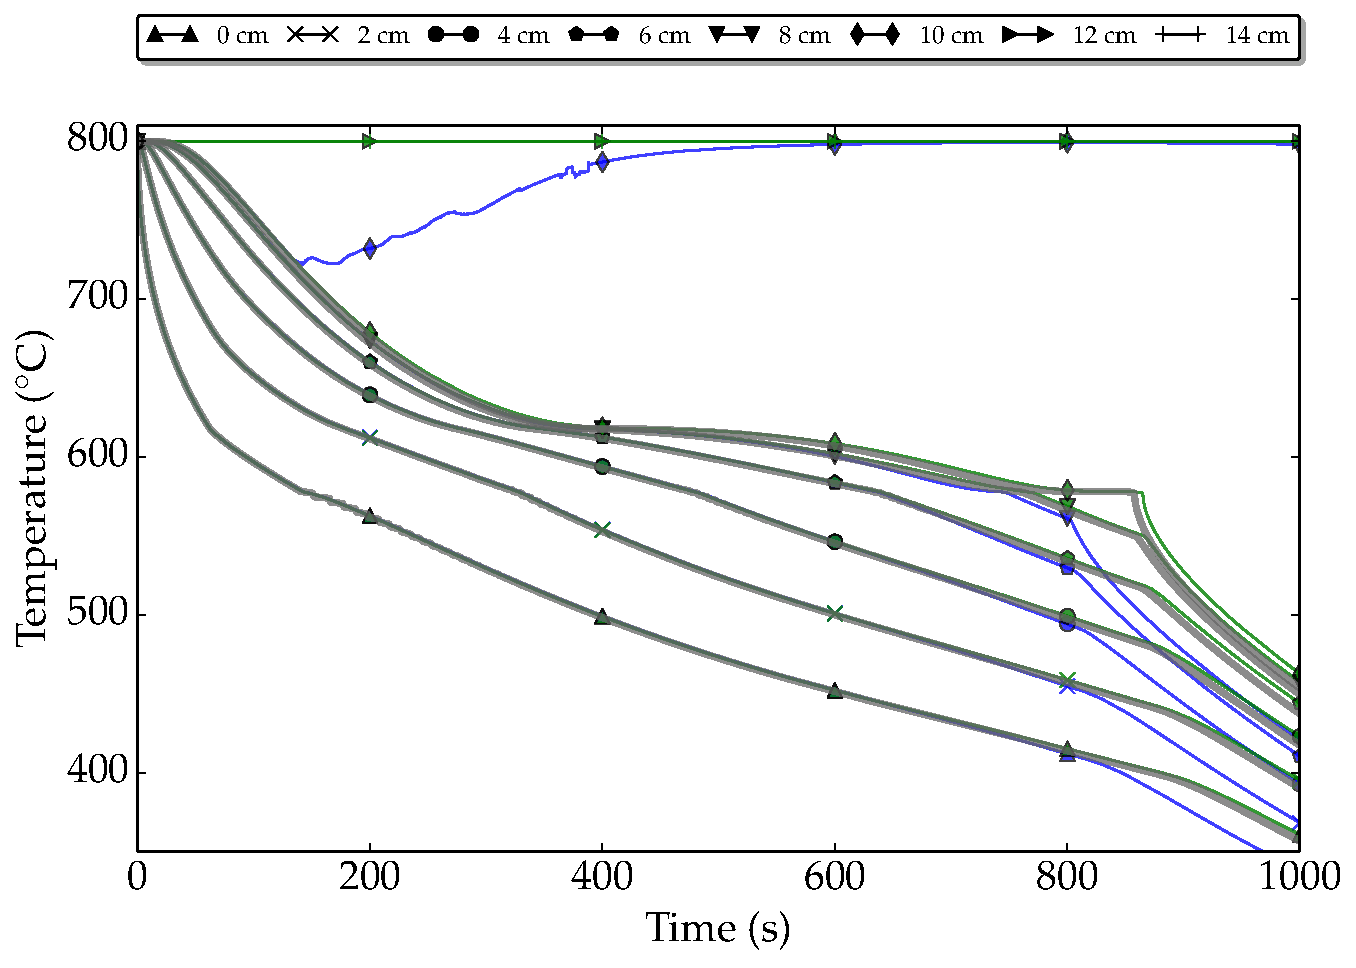
\includegraphics[width=\textwidth]{Chapter5/Data/1d_alsi7_cc/shrinkage_effect.pdf}
	\caption{Solidification shrinkage effect: grey curves correspond to a pure diffusion in a metal monodomain case,
			 \green{green} curves consider the latter case but with level set (metal and air domains) while \blue{blue} curves 
			 correspond to a shrinkage-driven flow case. All cases are solved without macrosegregation.}
    \label{fig:shrinkage_effect}
  \end{subfigure}
  %------------------------------
  \vskip\baselineskip
  %------------------------------
  \begin{subfigure}[t]{0.8\textwidth}
    \centering
	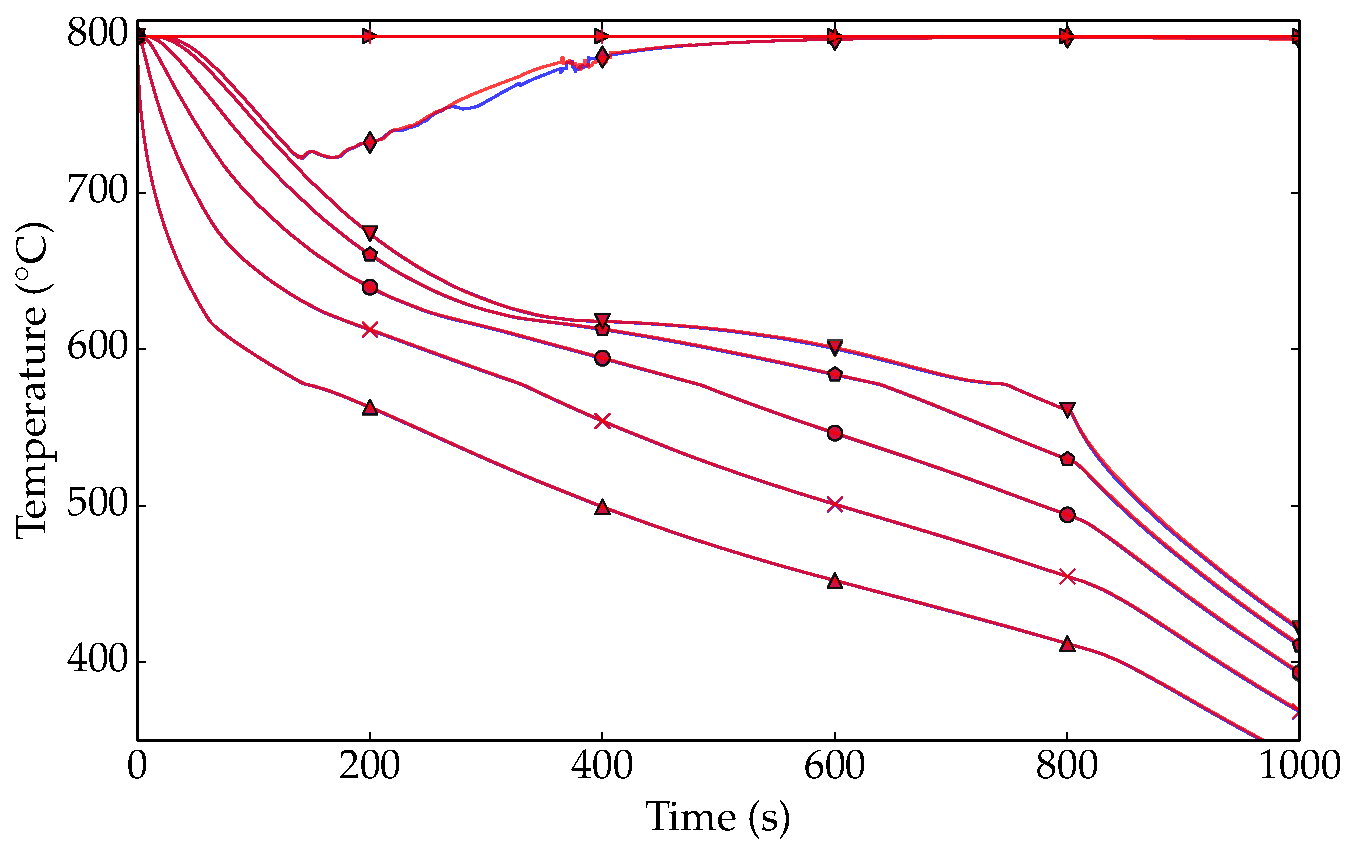
\includegraphics[width=\textwidth]{Chapter5/Data/1d_alsi7_cc/macro_effect.pdf}
	\caption{Macrosegregation effect: \blue{blue} curves represent the same simulation corresponding to the shrinkage-driven flow without macrosegregation, while
	the \red{red} curves correspond to a simulation of shrinkage-driven flow with macrosegregation.}
    \label{fig:macro_effect}
  \end{subfigure}
   %------------
\caption{Cooling curves at different fixed positions from 0 to 14 cm. 
where we show (a) the effect of solidification shrinkage on temperature history without any macrosegregation and
show (b) the effect of macrosegregation on temperature in the presence of solidification shrinkage.
Initial \emph{M-A} boundary: 10 cm.} 
\label{fig:1dalsi7_macro_shrinkage}
\end{figure}
%------------------

%--------------
\begin{figureth}
% textwidth 
{1.0}
%path 
{Chapter5/Graphics/1d/macro/gs_w.pdf}
% caption
{Zoom on the lower part, approximately 1.5 cm of the alloy close to the cooling boundary condition. 
The upper row of figures show the evolution of volume solid fraction, when eutectic transformation takes place. 
The vectors represent the direction of the average velocity field, with a length proportional
to the magnitude. The lower row of figures show for the same time increments, the solute redistribution, 
clearly changing behind the eutectic front.}
% label
\label{fig:1dalsi7_gs_w}
\end{figureth}
%--------------

\subsubsection{Shrinkage effect on average composition}
\Cref{fig:1dalsi7_gs_w} shows snapshots at different times of the shrinkage flow caused by the density difference between liquid and solid phases.
By solid phases, we mean the primary solid phase assumed as a dendritic structure, then the primary and secondary solid phases forming together the eutectic
that we see starting at 150 s in \cref{fig:1dalsi7_gs_w}. We can see that some solute segregation has already initiated in the mushy zone at 100 s.
However, the average composition reaches a positive peak of $\avg{w}$=\bin{Al}{7.4}{Si} with the initiation and progression of the eutectic front.
The sudden transformation of the remaining liquid in the mushy zone into eutectic solid, triggers a local velocity increase (real intrinsic velocity)
as each node's density varies from $\rhol$ to $\rhos$ in a single time step, at eutectic temperature. The velocity increase, shown later in \cref{fig:1dalsi7_dataVSlength},
causes species transport in the opposite direction of solidification, hence solute "freezes" in the eutectic structure leading to positive macrosegregation
in the first solidified nodes. This phenomenon is better known as inverse segregation. 
As the transport continues in the same direction, 
solute is progressively depleted in the remaining liquid, causing negative macrosegregation at nodes located between 2 cm and 7 cm from the cold wall.
\Cref{fig:1dalsi7_gs_w} shows only the first 1.5 cm of the solidifying sample, therefore a complete segregation profile is plotted along the sample length in \cref{fig:1dalsi7_wVSlength}a,
showing thus the negative macrosegregation as previously explained.
However, from 7 cm to the \emph{M-A} boundary, the average composition rises as clearly shown in \cref{fig:1dalsi7_wVSlength}a. This looks more like a numerical
instability than a physical rise in concentration. 
Bearing in mind that a reduced solute diffusion coefficient is imposed in the air domain \SI{1.5e-12}{\udiffusivity} compared to 
\SI{1.5e-9}{\udiffusivity} in the metal, we investigate into this instability by proposing two test cases: first, we try to limit the solute advection in the transition
zone where flow instabilities may form as seen previously in the segregation-free sample but keeping equal solute diffusion coefficients in both domains to \SI{1.5e-9}{\udiffusivity},
while for the second test case, we combine both low solute diffusion and low solute advection. The average composition results of these two test cases
are respectively plotted in \cref{fig:1dalsi7_wVSlength}b and \cref{fig:1dalsi7_wVSlength}c.
These results (second plot in \cref{fig:1dalsi7_wVSlength})  clearly show that just by reducing solute advection in the mixing zone reduce the amplitude of the composition instability.
In contrast, changing solute diffusion properties for the air coupled with reduced solute advection (third plot in \cref{fig:1dalsi7_wVSlength}) offers no further stability
in the segregation profile, which should normally stay below the nominal value near the interface.

%--------------------------------------
\shorthandoff{;:?!} %http://tex.stackexchange.com/questions/74860/unexpected-clash-between-babel-and-pgf-spy
\begin{figure}[htbp]
\centering
%-------
\begin{tikzpicture}%[spy using outlines={rectangle, magnification=3, width=1cm, height=6cm, connect spies}]
%[spy using outlines={circle, magnification=3, connect spies}]
  \begin{axis}
  [	name=one,
	title= (a),
	%at=(one.right of south east), anchor=left of south west,
	scale only axis,
	table/col sep=comma,  % comma % tab
	enlarge x limits=false,
	%legend pos=north east,
	scaled ticks=true,
	%xlabel=Sample length (m),
	ylabel=$\avg{w}$ (wt.\% Si),
	xticklabel style={/pgf/number format/fixed},
	xtick={0,0.02,...,0.14},
	xticklabels={},
	ytick={6.5,7,7.5},
	%x tick label style={rotate=45,anchor=east},
	width=0.9\textwidth,
	height=5cm,	
	ymin=6.45, ymax=7.55,
	%xmax=0.0928,
	mark repeat	= {142},
	cycle list name=mycycle, %exotic,
]
	\coordinate (spypoint) at (0.002,7.25);
	\coordinate (magnifyglass) at (0.06,7.3);
	\addplot table [x=arc_length, y=Concentration] {Chapter5/Data/1d_alsi7_composition/ModifyDiffSoluteAir.csv}; %\closedcycle ;
	%\addplot[thick, samples=50, smooth,magenta, name path=ls] coordinates {(0.09268,\pgfkeysvalueof{/pgfplots/ymin})(0.09268,\pgfkeysvalueof{/pgfplots/ymax})};
	\draw[thick, magenta,  opacity=0.5] (axis cs:0.0926,\pgfkeysvalueof{/pgfplots/ymin}) -- (axis cs:0.0926,\pgfkeysvalueof{/pgfplots/ymax});
	\draw[thick, dashed, black, opacity=0.5] (axis cs:\pgfkeysvalueof{/pgfplots/xmin},7) -- (axis cs:\pgfkeysvalueof{/pgfplots/xmax},7);
  	\end{axis}
%-------------------
 \begin{axis}
  [	name=two,
	title= (b),
	at=(one.below south west), anchor=above north west,
	scale only axis,
	table/col sep=comma,  % comma % tab
	enlarge x limits=false,
	%legend pos=north east,
	scaled ticks=true,
	%xlabel=Sample length (m),
	ylabel=$\avg{w}$ (wt.\% Si),
	xticklabel style={/pgf/number format/fixed},
	xtick={0,0.02,...,0.14},
	xticklabels={},
	ytick={6.5,7,7.5},
	%x tick label style={rotate=45,anchor=east},
	width=0.9\textwidth,
	height=5cm,	
	ymin=6.45, ymax=7.55,
	%xmax=0.0928,
	mark repeat	= {142},
	cycle list name=mycycle, %exotic,
]
	\addplot table [x=arc_length, y=Concentration] {Chapter5/Data/1d_alsi7_composition/ModifyVitLiq.csv}; %\closedcycle ;
	%\addplot[thick, samples=50, smooth,magenta, name path=ls] coordinates {(0.09268,\pgfkeysvalueof{/pgfplots/ymin})(0.09268,\pgfkeysvalueof{/pgfplots/ymax})};
	\draw[thick, magenta,  opacity=0.5] (axis cs:0.0926,\pgfkeysvalueof{/pgfplots/ymin}) -- (axis cs:0.0926,\pgfkeysvalueof{/pgfplots/ymax});
	\draw[thick, dashed, black, opacity=0.5] (axis cs:\pgfkeysvalueof{/pgfplots/xmin},7) -- (axis cs:\pgfkeysvalueof{/pgfplots/xmax},7);
  	\end{axis}
%-------------------
 \begin{axis}
  [	name=three,
	title= (c),
	at=(two.below south west), anchor=above north west,
	scale only axis,
	table/col sep=comma,  % comma % tab
	enlarge x limits=false,
	%legend pos=north east,
	scaled ticks=true,
	xlabel=Sample length (m),
	ylabel=$\avg{w}$ (wt.\% Si),
	xticklabel style={/pgf/number format/fixed},
	xtick={0,0.02,0.04,0.06,0.08,0.1,0.12,0.14},
	xticklabels={0,0.02,0.04,0.06,0.08,0.1,0.12,0.14},
	ytick={6.5,7,7.5},
	%x tick label style={rotate=45,anchor=east},
	width=0.9\textwidth,
	height=5cm,	
	ymin=6.45, ymax=7.55,
	%xmax=0.0928,
	mark repeat	= {142},
	cycle list name=mycycle, %exotic,
]
	\addplot table [x=arc_length, y=Concentration] {Chapter5/Data/1d_alsi7_composition/NewSolute.csv}; %\closedcycle ;
	%\addplot table [x=arc_length, y=Concentration] {Chapter5/Data/1d_alsi7_composition/ModifyVitLiq_ModifyDiffSoluteAir_NoSolute.csv}; %\closedcycle ;
	%\addplot[thick, samples=50, smooth,magenta, name path=ls] coordinates {(0.09268,\pgfkeysvalueof{/pgfplots/ymin})(0.09268,\pgfkeysvalueof{/pgfplots/ymax})};
	\draw[thick, magenta,  opacity=0.5] (axis cs:0.0926,\pgfkeysvalueof{/pgfplots/ymin}) -- (axis cs:0.0926,\pgfkeysvalueof{/pgfplots/ymax});
	\draw[thick, dashed, black, opacity=0.5] (axis cs:\pgfkeysvalueof{/pgfplots/xmin},7) -- (axis cs:\pgfkeysvalueof{/pgfplots/xmax},7);
  	\end{axis}
%\spy [black] on (spypoint) in node[fill=white] at (magnifyglass);  
\end{tikzpicture}
%-------
\caption{Plot of the average composition as function of length, along a vertical line passing through the centre of the sample at 1000 s, with 
		(a) low solute diffusion in the air but unmodified solute advection (minimum composition reaches \SI{2.2}{\ucomposition} Si but not shown), 
		(b) reduced solute advection in the level set transition zone or (c) a combination of the previous
		techniques. The solid magenta line shows the position of the interface after solidification 
		while the black dashed line shows the nominal average composition of the alloy.}
\label{fig:1dalsi7_wVSlength}
\end{figure}
%--------------------------------------
\shorthandon{;:?!} %http://tex.stackexchange.com/questions/74860/unexpected-clash-between-babel-and-pgf-spy


%=====================================BIG LANDSCAPE FIGURE =====================================
\begin{landscape}
\begin{figureth}
% textwidth 
{1.5}
%path 
{Chapter5/Data/1d_alsi7_arc_compositions/compositions_vs_length.pdf}
% caption
{Group of plots where each row is a given time increment (t=200 s, t=600 s and t=800 s) of the 1D solidification shrinkage simulation with macrosegregation, 
while each column one or more physical quantities are plotted along a vertical line passing through the centre of the sample. Plots are titled with the corresponding plotted quantities.}
% label
\label{fig:1dalsi7_dataVSlength}
\end{figureth}
\end{landscape}
%=====================================BIG LANDSCAPE FIGURE =====================================

The plots in \cref{fig:1dalsi7_dataVSlength} give important information on the segregation shown in  \cref{fig:1dalsi7_gs_w}.
CONTINUE COMMENTING ON \cref{fig:1dalsi7_dataVSlength}.


\subsubsection{Solute mass conservation}

Show solute mass conservation with equal or low solute diffusion in air








\cleardoublepage
% **********************************************************************
\section{2D application: controlled solidification benchmark}
% **********************************************************************
In this application, we aim at predicting macrosegregation produced by liquid convection, in the presence of solidification shrinkage.
An molten alloy is put in a rectangular crucible with controlled cooling flux on one or two sides to the crucible. The importance of the experiment lies in the 
thermal convection forces arising from temperature gradients, but also solutal buoyancy forces arising from liquid concentration gradients. The final macrosegregation pattern
strongly depends on density variations caused by each chemical species, but also on the experimental conditions like the lateral thermal gradients as well the cooling rate,
as shown in \cref{fig:smacs_exp}.
\citet{hebditch_observations_1974} suggested one of the first experiments working on Sn-Zn and Sn-Pb alloys. 
More recently, an experimental benchmark was performed by \citet{hachani_experimental_2012} to obtain more accurate 
composition results with various Sn-Pb and Pb-Sn alloys. In the current section, we are interested in the latter experiment, especially in the prediction
of the metal's shrunk surface together with the final macrosegregation.

%
%-----------------
\begin{figure}[htbp]
\centering
   %------------
  \begin{subfigure}[t]{0.45\textwidth}
    \centering
	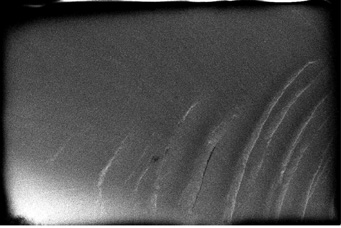
\includegraphics[width=\textwidth]{Chapter5/Graphics/2d/Hachani0p02.png}
	\caption{}
    \label{fig:smacs_lowcr}
  \end{subfigure}
  %------------------------------
  \hfill
  %------------------------------
  \begin{subfigure}[t]{0.45\textwidth}
    \centering
	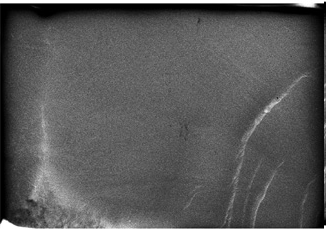
\includegraphics[width=\textwidth]{Chapter5/Graphics/2d/Hachani0p04.png}
	\caption{}
    \label{fig:smacs_highcr}
  \end{subfigure}
   %------------
\caption{Final macrosegregation patterns obtained by solidifying a \bin{Sn}{3}{Pb} alloy at (a) \SI{0.02}{\uCR} and (b) \SI{0.04}{\uCR}. 
The different cooling rates result in different lead segregation patterns, with a greater number of channel segregates in the latter.
The X-rays show also a visible sign of volume shrinkage at the top of each ingot \citep{hachani_experimental_2012}.}
\label{fig:smacs_exp}
\end{figure}
%------------------


% %**********************************
% \subsection{Absence of convection}
% %**********************************
% We first try to simulate the solidification process by neglecting thermosolutal dependence of phase densities in the Navier-Stokes solver. By doing so,
% no convection forces should arise during solidification, 
% hence the generated flow is only due to the difference between solid and liquid densities, that is the shrinkage driving force.

% ********************************************
\subsection{Boundary condition effect}
% ********************************************

First, we want to understand the consequence of removing the no-slip boundary condition at the \emph{M-A} boundary and compare the effect on macrosegregation. 
For computations without level set, as previously done in chapter 4 for the \emph{Tsolver}'s validation in convection-diffusion regimes, a no-slip condition was applied for all domain boundaries including 
the interface.
However, this is not readily implemented with the level set method which considers the local interface velocity for its transport.
In \cref{fig:slipbc_2800,fig:slipbc_7000}, we compare at 2800 s and 7000 s the differences between a no-slip condition on the top boundary 
and a free-slip tangential condition, assuming zero normal velocity. 

%-----------------
\begin{figure}[htbp]
\centering
   %------------
  \begin{subfigure}[t]{0.4\textwidth}
    \centering
  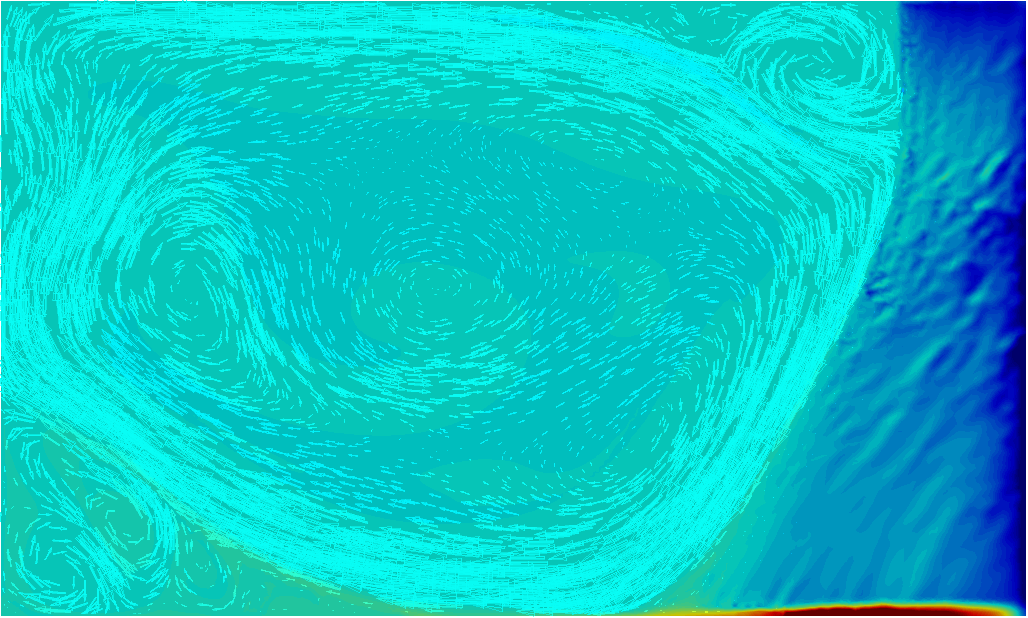
\includegraphics[width=\textwidth]{Chapter5/Graphics/2d/ref_2800s_nosliptop.png}
  \caption{}
    \label{fig:noslip2800}
  \end{subfigure}
  %------------------------------
  \begin{subfigure}[t]{0.15\textwidth}
    \centering
  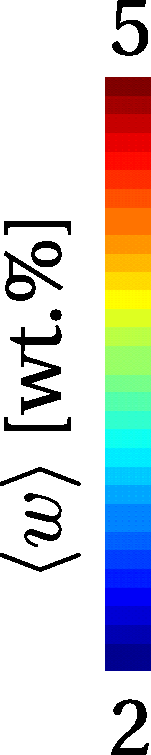
\includegraphics[width=0.3\textwidth]{Chapter5/Graphics/2d/colorbar.pdf}
  \end{subfigure}
  %------------------------------
  \begin{subfigure}[t]{0.4\textwidth}
    \centering
  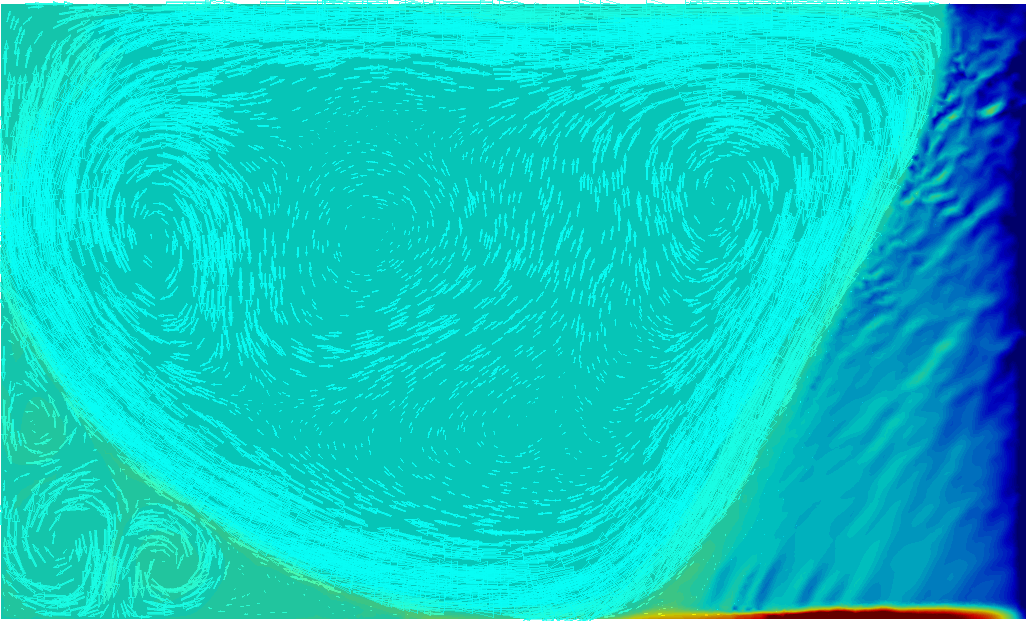
\includegraphics[width=\textwidth]{Chapter5/Graphics/2d/ref_2800s_sliptop.png}
  \caption{}
    \label{fig:freeslip2800}
  \end{subfigure}
   %------------
\caption{Comparison of two solidification with macrosegregation cases assuming (a) a no-slip condition on the upper boundary 
or (b) a tangential free-slip condition. The snapshots are taken at 2800 s.}
\label{fig:slipbc_2800}
\end{figure}
%------------------

%-----------------
\begin{figure}[htbp]
\centering
   %------------
  \begin{subfigure}[t]{0.4\textwidth}
    \centering
  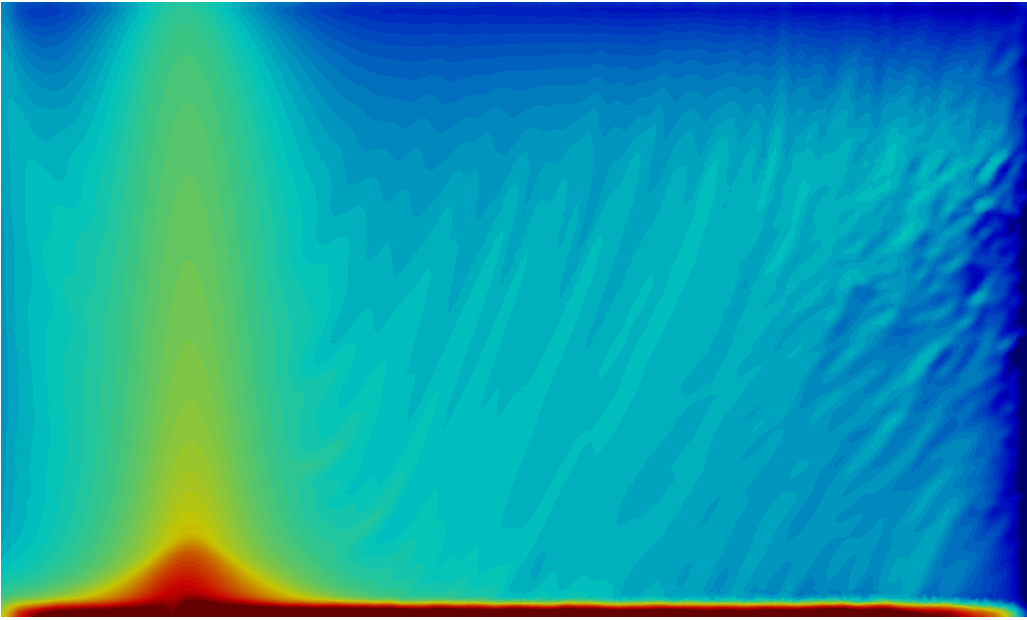
\includegraphics[width=\textwidth]{Chapter5/Graphics/2d/ref_7000s_nosliptop.png}
  \caption{}
    \label{fig:noslip7000}
  \end{subfigure}
  %------------------------------
  \begin{subfigure}[t]{0.15\textwidth}
    \centering
  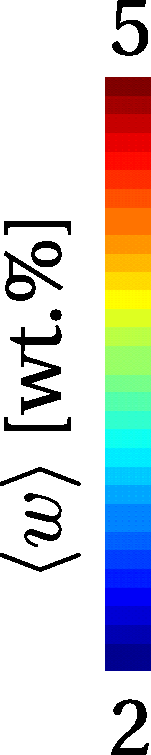
\includegraphics[width=0.3\textwidth]{Chapter5/Graphics/2d/colorbar.pdf}
  \end{subfigure}
  %------------------------------
  \begin{subfigure}[t]{0.4\textwidth}
    \centering
  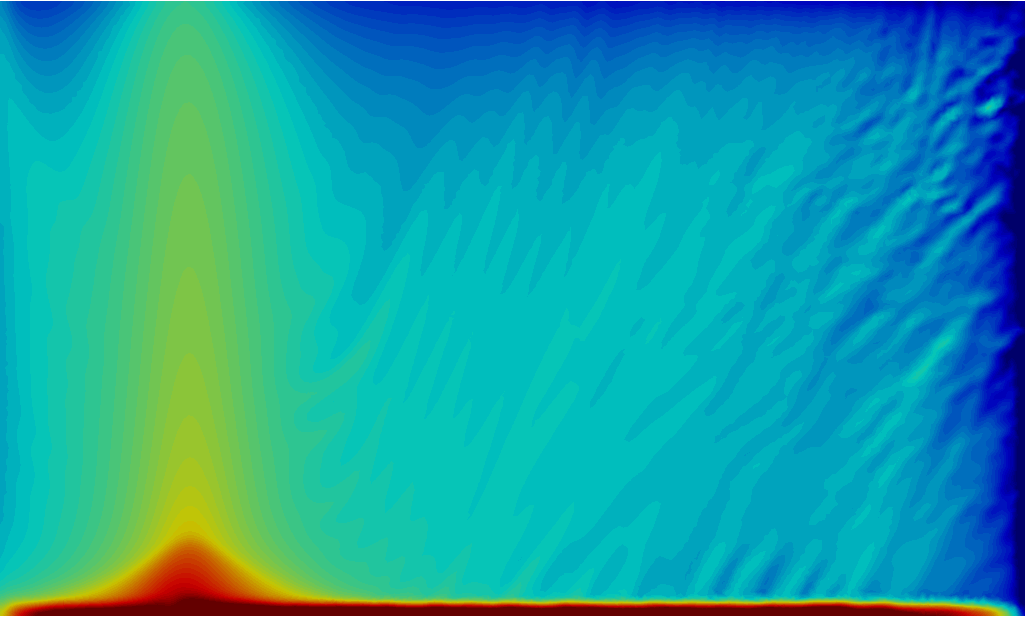
\includegraphics[width=\textwidth]{Chapter5/Graphics/2d/ref_7000s_sliptop.png}
  \caption{}
    \label{fig:freeslip7000}
  \end{subfigure}
   %------------
\caption{Comparison of two solidification with macrosegregation cases assuming (a) a no-slip condition on the upper boundary 
or (b) a tangential free-slip condition. The snapshots are taken at 7000 s.}
\label{fig:slipbc_7000}
\end{figure}
%------------------

In \cref{fig:slipbc_2800}, solidification is still at an early stage, at 2800 s. The main difference between \cref{fig:noslip2800} and 
\cref{fig:freeslip2800} is the flow pattern near the top interface. The no-slip wall acts a brake for the vicinity flow, 
deviating it downwards and allow a quicker solidification rate for the right upper part of the metal. The flow near the slip wall
in \cref{fig:freeslip2800} is not damped and therefore delays solidification of the upper corner where it impinges.
The different flow pattern creates a more pronounced negative segregation in the upper right corner of \cref{fig:noslip2800}, compared
to the same location in  \cref{fig:freeslip2800}. Later when solidification is complete at 7000 s (\cref{fig:slipbc_7000}), the overall
macrosegregation is more visible: expect for the previously mentioned difference in the corner segregation, no big differences are observed.
This means that when using the level set method, allowing the velocity to have non-zero values near the interface should not drastically  change the
predicted flow pattern and the subsequent macrosegregation.

% ********************************************
\subsection{Computational configuration}
% ********************************************


% -------------------------------------------
\subsubsection{Mesh and adaptive remeshing}
% -------------------------------------------
The case considers a 2D geometry having equivalent dimensions to the 3D case performed earlier (sample of 10 cm in length and 6 cm in height).
To accomodate the air domain, an extra 2 cm are added to sample's height, which finally reaches 8 cm, the interface is thus kept at an elevation of 6 cm. 
The inital mesh consists of three different mesh sizes: isotropic meshes in the air and the metal, having respectively a uniform size of 2 mm and 1 mm.
Regarding the interface, an anisotropic mesh adapts to the \emph{M-A} boundary with a mesh size of 0.1 mm in the normal direction to the interface.
The thickness of the anisotropic mesh spans 0.5 mm from each side of the interface.

To adapt the mesh, we use the \emph{Remesh4} adaptive technique to maintain accurate predictions for velocity and interface transport.
However as solidification proceeds, we also need to keep a relatively small mesh size in regions with noticeable composition gradients.
Although this is possible with the \emph{Remesh4} technique, it is more difficult to maintain a fine mesh size throughout the metal, especially in areas
where solidification is almost complete and the velocity field is has a low magnitude. The consequence is a loss of information when coarser 
elements are obtained by remeshing.

To avoid such unwanted effects, we use another uniform
isotropic grid, named \emph{grid B}, having a constant mesh size of 0.3 mm, that is three times smaller than the interface elements in the original mesh (named \emph{grid A}).
The strategy consists of scanning the liquid fraction of each node in \emph{grid A}, if its value is located between 30\% and 70\%, then we consider that is a 
a region of interest, since the flow velocity is still not zero and a relatively fine mesh is locally obtained. 
We consequently transport the average composition field exclusively 
for these nodes from \emph{grid A} to \emph{grid B}, keeping for all other nodes their respective average composition values.
It should be noted that this transport is only one-way, hence no information feedback from \emph{grid B} to \emph{grid A}.

%-----------------
\begin{figure}[htbp]
\centering
   %------------
  \begin{subfigure}[t]{0.3\textwidth}
    \centering
    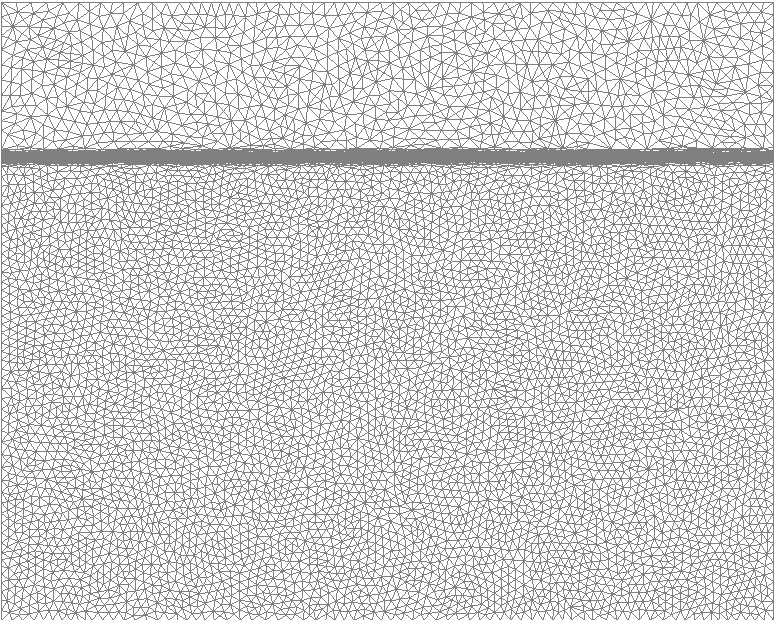
\includegraphics[width=\textwidth]{Chapter5/Graphics/2d/GridAinit.png}
    \caption{\emph{Grid A} (initial)}
    \label{fig:gridAinit}
  \end{subfigure}
  %------------------------------
  \begin{subfigure}[t]{0.3\textwidth}
    \centering
    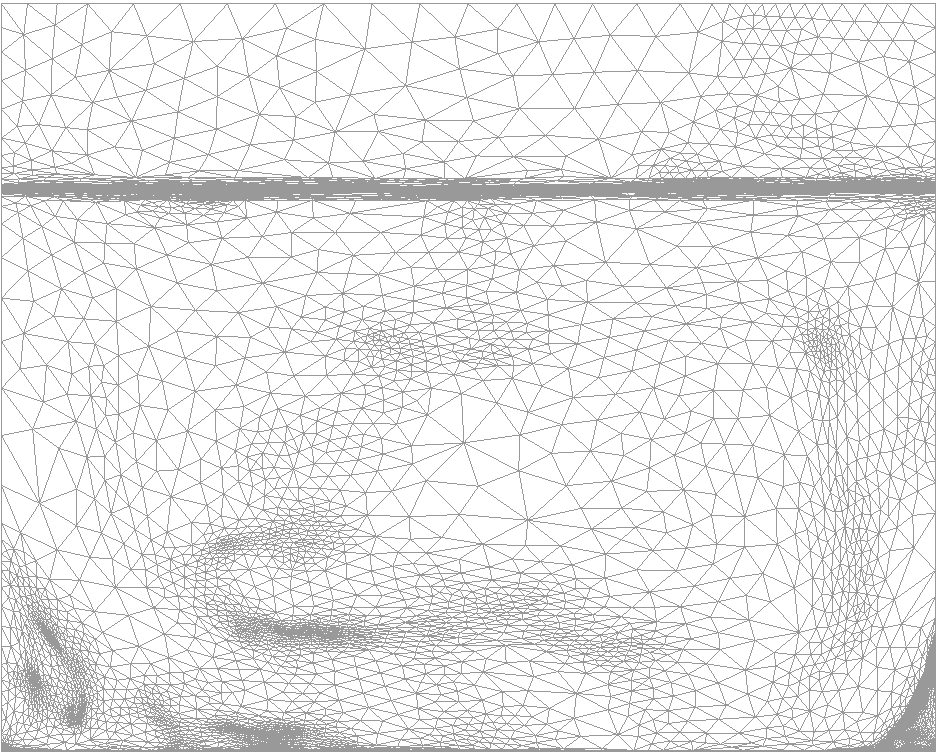
\includegraphics[width=\textwidth]{Chapter5/Graphics/2d/GridA.png}
    \caption{\emph{Grid A}}
    \label{fig:gridA}
  \end{subfigure}
  %------------------------------
  \begin{subfigure}[t]{0.3\textwidth}
    \centering
    
\includegraphics[width=\textwidth]{Chapter5/Graphics/2d/GridB.png}
    \caption{\emph{Grid B}}
    \label{fig:gridB}
  \end{subfigure}
   %------------
\caption{Snapshots of (a) the initial adaptive anisotropic \emph{grid A} then (b) the same grid but at 
a given time increment with (c) the corresponding fixed isotropic \emph{grid B} at the same time increment.}
\label{fig:smacs_grids}
\end{figure}
%------------------


% -----------------------------------------------
\subsubsection{Initial and boundary conditions}
% -----------------------------------------------
The air initial temperature is the same as the initial liquid. This is only a hypothesis to prevent steep temperature gradients at the interface,
which may lead to surface solidification. The initial and boundary thermal conditions used to cool down the metal are defined in chapter 4, given by the experimental
data of \citet{hachani_experimental_2012}. For the mechanical properties, the top wall allows free inflow/outflow of the air in all directions 
at an imposed atmospheric pressure.
This allows the air to follow any volume changes in the metal upon solidifying and shrinking. 

The side walls adjacent to the heat exchangers are given a free tangential slip boundary condition but with a zero normal velocity, which lets the transported 
level set function move vertically without being attached to the sides. Finally, a no-slip condition applies to the bottom wall. 


% ********************************************
\subsection{Results}
% ********************************************

The results are recorded at two intermdiate solidification stages, at 3050 s and 3550 s, knowing that solidification onset is around 1920 s.
First, we look to the results in \cref{fig:W_mask_1200s}. The original average composition field obtained by \emph{grid A}, shown in \cref{fig:1200s_compo},
is almost free of composition gradients except for one segregated channel rising from the bottom by the action of thermal convection.
On the other hand, the average composition transport from the adaptive grid to the fixed one, allows recording macrosegregation onto the latter
at nodes where the solid exceeds 0.7 in volume fraction, depicted by the yellow region in \cref{fig:1200s_unmask}. 
This is why we observe in \cref{fig:1200s_compobis} a number of channel segregates
which are slightly below nominal composition but still richer in lead species with respect to the surrounding solid.
The solid fraction distribution is shown in \cref{fig:1200s_gs}, along with the flow pattern. Local vortices are observed in the metal, probably due 
to considering only a 2D geometry instead of the complete 3D, and this alters the computation stability by ignoring the boundary layers in the sample 
thickness, obtained otherwise in 3D. Nevertheless, the overall 
flow is driven by a thermosolutal driving force, with a compatible flow in the air side. 
We can observe how the solid fraction is modified in the segregated channel, as a result of macrosegregation.
At this stage of solidification, the interface movement is still difficult to see, but 500 s later it becomes more visible.

%-----------------
\begin{figure}[htbp]
\centering
   %------------
  \begin{subfigure}[t]{0.4\textwidth}
    \centering
  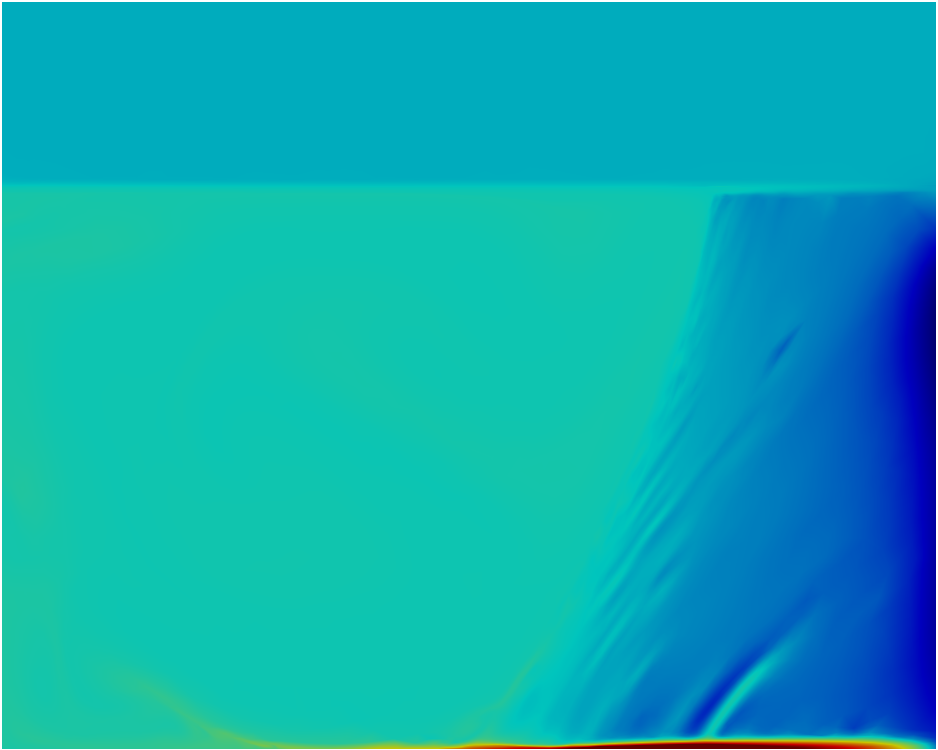
\includegraphics[width=\textwidth]{Chapter5/Graphics/2d/1200s_compo.png}
  \caption{Lead composition on \emph{Grid A}}
    \label{fig:1200s_compo}
  \end{subfigure}
  %------------------------------
  \begin{subfigure}[t]{0.15\textwidth}
    \centering
  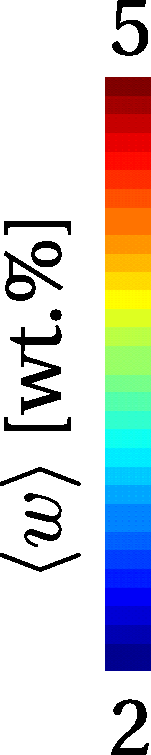
\includegraphics[width=0.3\textwidth]{Chapter5/Graphics/2d/colorbar.pdf}
  \end{subfigure}
  %------------------------------ 
  \begin{subfigure}[t]{0.4\textwidth}
    \centering
  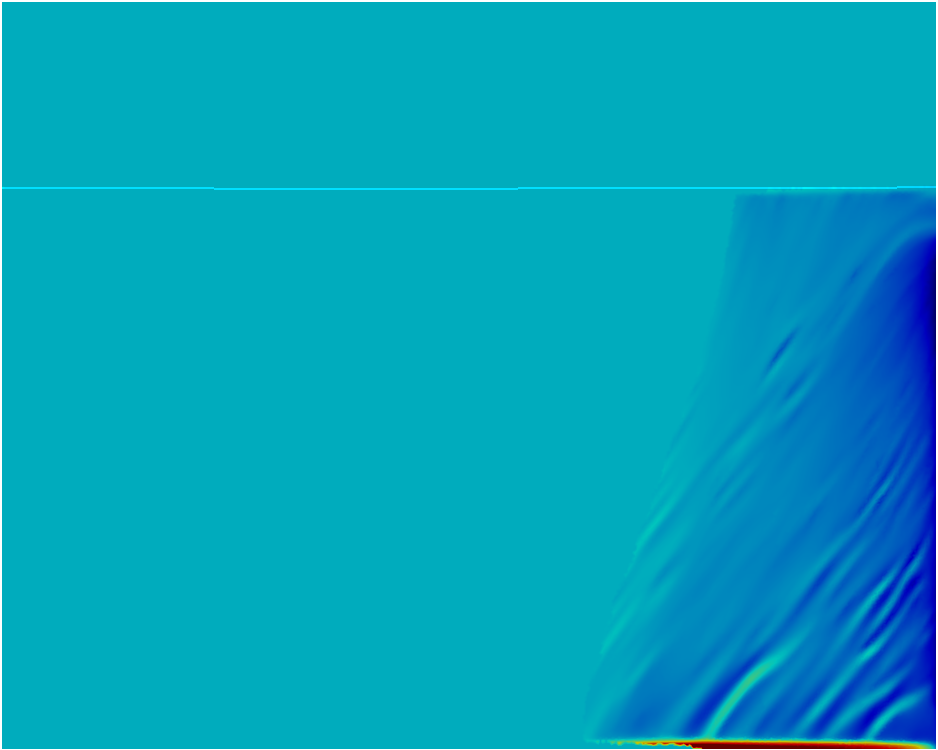
\includegraphics[width=\textwidth]{Chapter5/Graphics/2d/1200s_compobis.png}
  \caption{Lead composition on \emph{Grid B}}
    \label{fig:1200s_compobis}
  \end{subfigure}
   %------------
   \vspace{5mm}
   %------------------------------
  \begin{subfigure}[t]{0.4\textwidth}
    \centering
  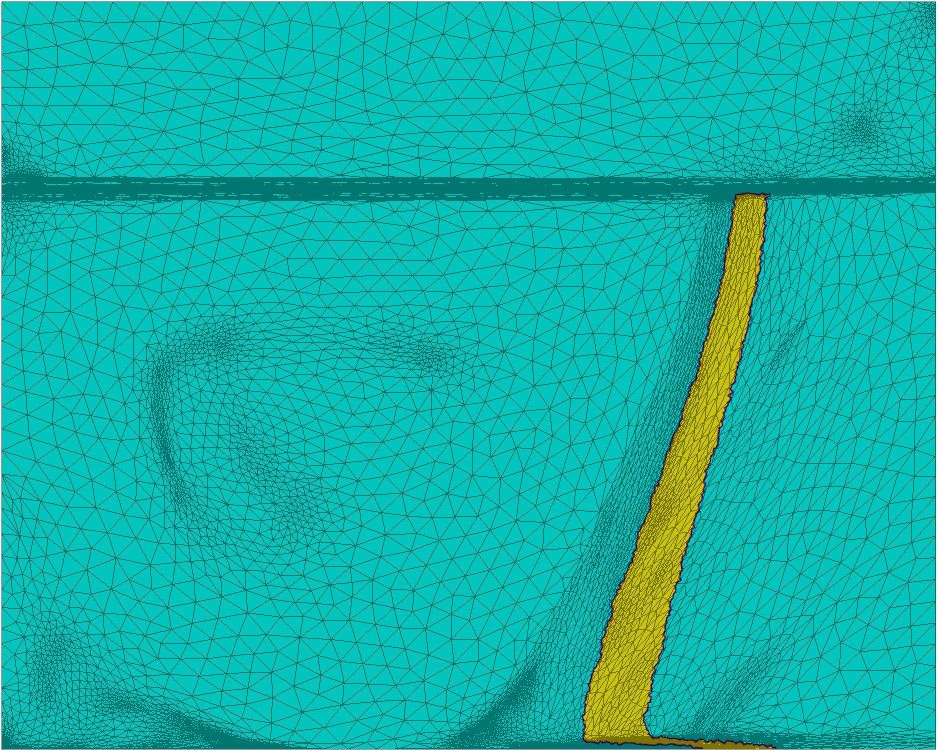
\includegraphics[width=\textwidth]{Chapter5/Graphics/2d/1200s_unmask.png}
  \caption{Transport from \emph{grid A} to \emph{grid B}}
    \label{fig:1200s_unmask}
  \end{subfigure}
   %------------
   %------------
   %------------------------------
  \begin{subfigure}[t]{0.15\textwidth}
    \centering
  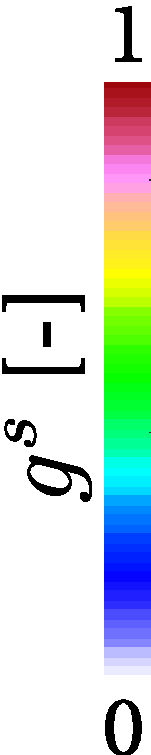
\includegraphics[width=0.3\textwidth]{Chapter5/Graphics/2d/colorbar_gs.pdf}
  \end{subfigure}
  %------------------------------
  %------------------------------
  \begin{subfigure}[t]{0.4\textwidth}
    \centering
  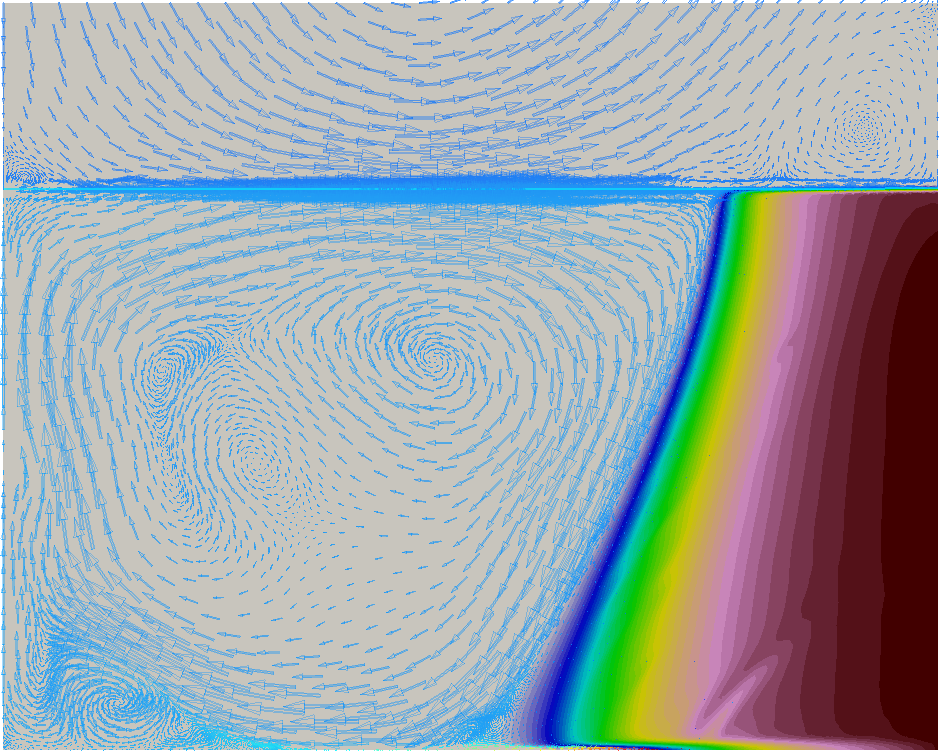
\includegraphics[width=\textwidth]{Chapter5/Graphics/2d/1200s_gs_vl.png}
  \caption{Solid fraction on \emph{grid B}}
    \label{fig:1200s_gs}
  \end{subfigure}
\caption{Snapshots at 3050 s of the average composition field shown on (a) \emph{grid A} where the mesh gets coarser in fully solidified regions near the right side while
and then on (b) \emph{grid B} where the uniform fine mesh predicts a smoother composition field (line indicates the current interface level). 
The increased number of segregated channels on the right side of the
metal is obtained by the successive transport operations performed in (c) a restricted area (\yellow{yellow} color) based on the nodal values of (d) the solid fraction field.}
\label{fig:W_mask_1200s}
\end{figure}
%------------------


We are now at 3550 s, and the decreasing left heat exchanger temperature has just went below the local liquidus, 
triggering solidification from the left side.
The average composition field presents noticeable differences between the adaptive \emph{grid A} and the fixed \emph{grid B}.
The weak macrosegregation observed in \cref{fig:1200s_compo} are now lost in \cref{fig:1700s_compo}, as the mesh got coarser on the metal's solidified right
side. Fortunately, the macrosegregation distribution is stored in the fixed grid (\cref{fig:1700s_compobis}) and shows more details with the advancement of solidification. 
The shrinkage due to phase density difference, is now clearly visible judging from interface shape, which still almost planar above the last liquid pool. 

%-----------------
\begin{figure}[htbp]
\centering
   %------------
  \begin{subfigure}[t]{0.4\textwidth}
    \centering
  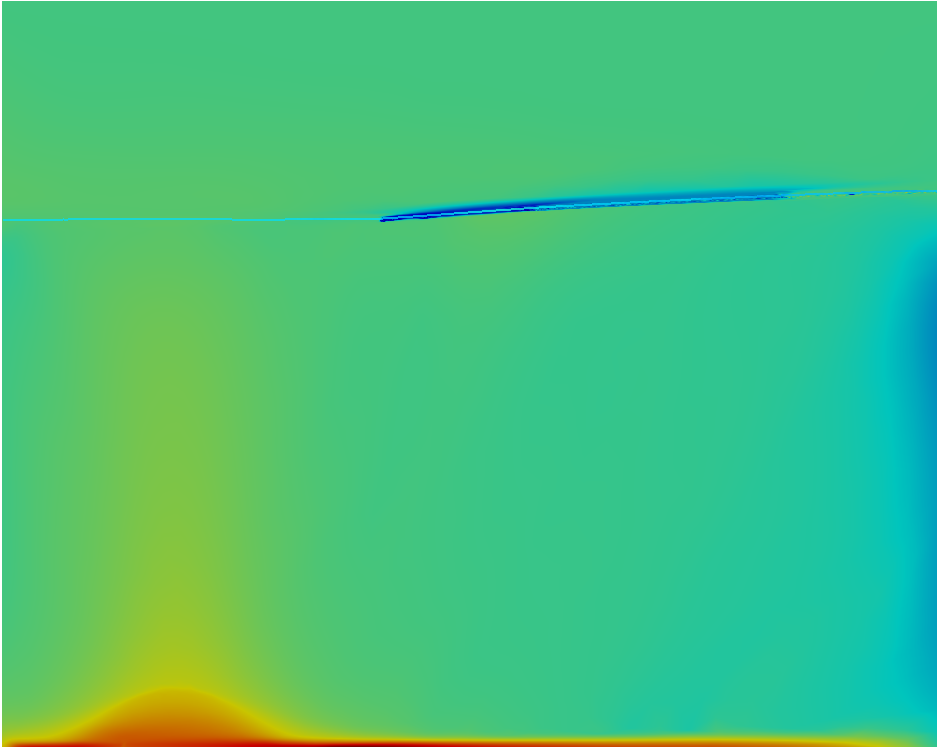
\includegraphics[width=\textwidth]{Chapter5/Graphics/2d/1700s_compo.png}
  \caption{Lead composition on \emph{Grid A}}
    \label{fig:1700s_compo}
  \end{subfigure}
  %------------------------------
  \begin{subfigure}[t]{0.15\textwidth}
    \centering
  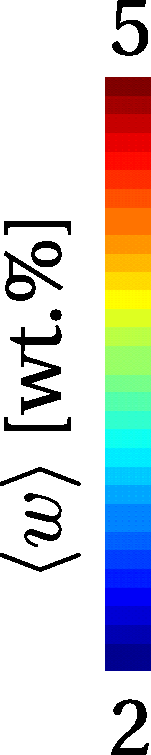
\includegraphics[width=0.3\textwidth]{Chapter5/Graphics/2d/colorbar.pdf}
  \end{subfigure}
  %------------------------------ 
  \begin{subfigure}[t]{0.4\textwidth}
    \centering
  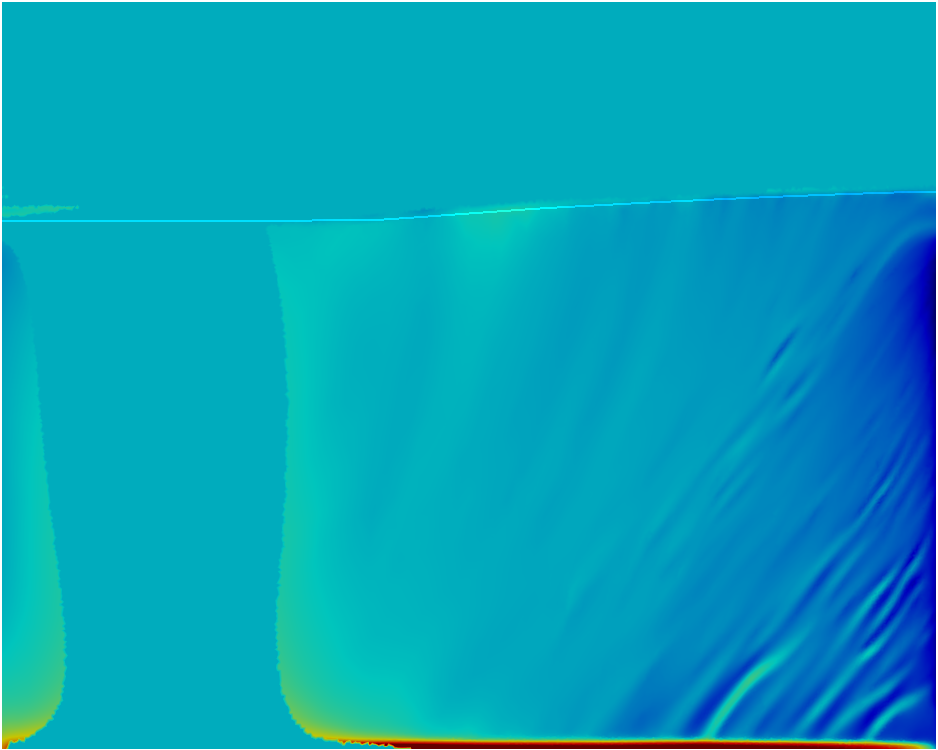
\includegraphics[width=\textwidth]{Chapter5/Graphics/2d/1700s_compobis.png}
  \caption{Lead composition on \emph{Grid B}}
    \label{fig:1700s_compobis}
  \end{subfigure}
   %------------
   \vspace{5mm}
   %------------------------------
  \begin{subfigure}[t]{0.4\textwidth}
    \centering
  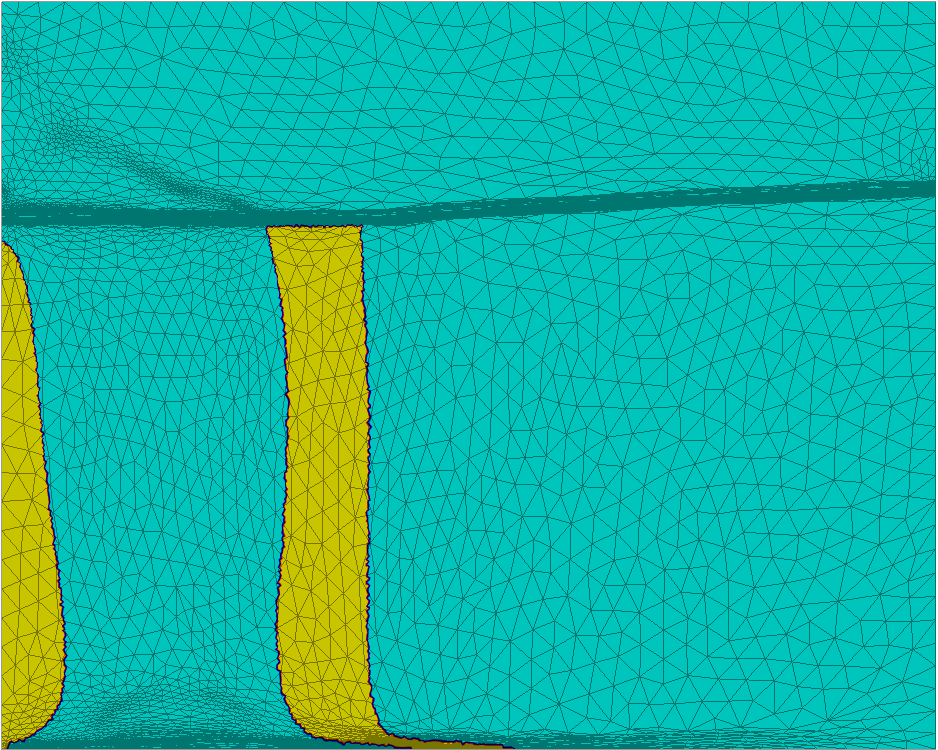
\includegraphics[width=\textwidth]{Chapter5/Graphics/2d/1700s_unmask.png}
  \caption{Transport from \emph{grid A} to \emph{grid B}}
    \label{fig:1700s_unmask}
  \end{subfigure}
   %------------
   %------------
   %------------------------------
  \begin{subfigure}[t]{0.15\textwidth}
    \centering
  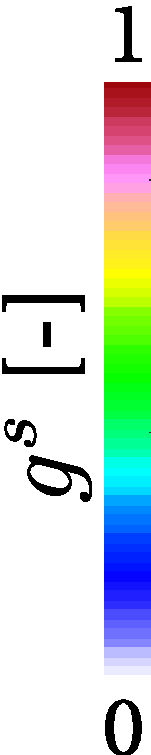
\includegraphics[width=0.3\textwidth]{Chapter5/Graphics/2d/colorbar_gs.pdf}
  \end{subfigure}
  %------------------------------
  %------------------------------
  \begin{subfigure}[t]{0.4\textwidth}
    \centering
  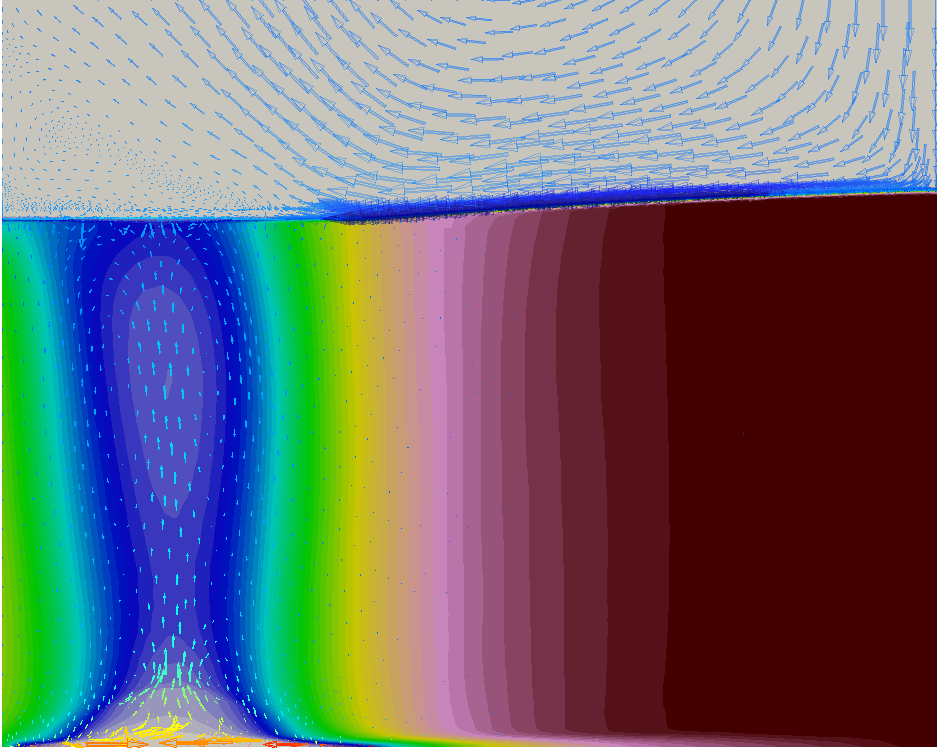
\includegraphics[width=\textwidth]{Chapter5/Graphics/2d/1700s_gs_vl.png}
  \caption{Solid fraction on \emph{grid B}}
    \label{fig:1700s_gs}
  \end{subfigure}
\caption{Snapshots at 3550 s of (a) the average composition result obtained on \emph{grid A}, compared to (b) the composition field obtained on \emph{grid B}, 
(c) theafter being transported in (c) a restricted area (\yellow{yellow} color) based on the nodal values of (d) the solid fraction field.}
\label{fig:W_mask_1700s}
\end{figure}
%------------------



%--------------
\begin{figureth}
% textwidth 
{0.75}
%path 
{Chapter5/Graphics/2d/finalseg/finalsegreg.pdf}
% caption
{blabl}
% label
\label{fig:smacs_final}
\end{figureth}
%--------------



























% --------------------------------------------------------------------------------------------------------------------------
\cleardoublepage
% ---------------------------------
\section{3D application: reduced-gravity solidification}
% ---------------------------------

% ---------------------------------
%\subsection{Introduction}
% ---------------------------------
As presented in the introductory chapter, the aim of the CCEMLCC project is to "reach a better
understanding of surface defects formed during processing of steels from the liquid state" \citep{gandin_project_2014}.
Among the several scientific topics being studied, the interaction between skin macrosegregation 
and thermomechanical deformation is investigated through chill cooling experiments.
The idea is to have the molten steel in a containerless environment, which could be done by several ways: 
electromagnetic levitation, on-board parabolic flights or sounding rockets and finally
in a real microgravity context as in the ISS. Heat is extracted from the sample by contact with a ceramic 
(Si$_3$N$_4$) substrate at room temperature (hence the term "chill cooling"), that collides into the alloy at a controlled speed.
This contact situation generating a high thermal gradient is comparable to casting processes between the molten alloy and the moulds.
For ground-based experiments, EML was used to achieve chill cooling of samples without using moulds. 
However, levitation induces currents in the spherical sample, generated by means of electromagnetic stirring (Lorentz forces) 
but also by thermal and solutal convection on the other hand. In reduced-gravity conditions, the dynamics of the phenomena behind fluid motion are less significant.
The current modelling is therefore compared to chill cooling experiments performed in parabolic flights and sounding rockets 
with reduced gravitational forces ($\norm{\gravity} \in \crochet{10^{-1};10^{-5}}$\si{\uacceleration}).


% ---------------------------------
\subsection{Previous work}
% ---------------------------------

% ---------------------------------
\subsubsection{TEMPUS experiment for parabolic flight campaigns}
% ---------------------------------

The TEMPUS experiment came as a first alternative for EML experiments on ground during which accurate thermophysical and rheological characterisation were difficult to achieve.
Each flight consists of several cycles of free fall, a reduced-gravity environment is hence created, 
allowing to use only a single radiofrequency (RF) coil to stabilise the position of the droplet, while the substrate comes into contact with the molten sample
from above it. An axial pyrometer measures the sample temperature during the process. 
Also, a high-speed camera records the solidification process, producing frames as shown in \cref{fig:camera}.
This is useful to measure the front growth speed. 
Each parabola cycle lasts for 50 s, offering an effective low gravity ($\norm{\gravity}\approx$\SI{e-1}{\uacceleration}) for about 20 s.

% ---------------------------------
\subsubsection{TEXUS sounding rocket}
% ---------------------------------

TEXUS-46 is the name of the sounding rocket mission that carries the experimental setup, 
but for simplicity we will refer to the latter as being the TEXUS experiment. The setup is shown in \cref{fig:texus_exp}.
The main difference with respect to parabolic flight experiments,
TEXUS features solidification in near-zero gravitational fields and for extended periods of time (3 minutes). 
We do not have an exact measurement of the gravitational field magnitude, but it is several orders
less than Earth's gravity magnitude ($\norm{\gravity} \in \crochet{10^{-5};10^{-8}}$\si{\uacceleration}).
It should be mentionned that the experimental setup is comparable between parabolic flights and sounding rocket experiments. That is to say
that the dimensions of the steel sample, the substrate and the container are almost the same. Nevertheless, different steel compositions were
considered in each type of experiment.

%--------------
\begin{figureth}
% textwidth 
{1.0}
%path 
{Chapter5/Graphics/3d/exp.pdf}
% caption
{Three frames describing the experimental setup used to achieve reduced-gravity 
solidification on-board a sounding rocket flight,
showing the initial alloy sample, the cage and the positiong coil. The setup
is similar to the one used for TEMPUS experiments.}
% label
\label{fig:texus_exp}
\end{figureth}
%--------------

%--------------
\begin{figureth}
% textwidth 
{1.0}
%path 
{Chapter5/Graphics/3d/camera.pdf}
% caption
{Image sequence given by a high speed camera on-board a TEMPUS parabolic flight (parabola \#14 Oct 2014), showing the 
solidification progress between 0 s (when contact with the chill is initiated) to 3.75 s in a \tern{Fe}{0.9}{C}{0.2}{Si} steel droplet. 
The progress of the solidification front is marked by the green dashed line. In some frames, the droplet is partially hidden by the narrow 
opening of the sample holder facing the camera.}
% label
\label{fig:camera}
\end{figureth}
%--------------

%--------------
\begin{figureth}
% textwidth 
{0.4}
%path 
{Chapter5/Graphics/3d/camera_end.pdf}
% caption
{Camera image from the TEMPUS 2014 experiment, showing the fully solidified droplet with a deformed shape after 10 s.}
% label
\label{fig:camera_end}
\end{figureth}
%--------------

% --------------------------------------
\subsubsection{Numerical contribution}
% --------------------------------------

A former numerical contribution was done by \citet{rivaux_simulation_2011} at CEMEF, as mentioned in the first chapter. 
His model considered both the steel droplet and the ceramic chill in a Lagrangian formulation, i.e. each object is
modelled using a separate mesh. Conservation equations of mass, energy,
chemical species and momentum were solved in the metal domain, while the energy
conservation was the sole equation solved on the chill mesh. The mechanical problem was divided
into two parts: fluid mechanics and solid mechanics. 
For the first part, the momentum conservation in the liquid phase was solved using an
incompressible P1/P1 SUPG-PSPG formulation of Navier-Stokes equations, i.e. 
without any contraction for the liquid phase neither solidification shrinkage at the solid-liquid interface.
The second part, solid mechanics, was solved using P1+/P1 formulation to predict solid deformation caused by the 
solid's thermal contraction as well as solidification shrinkage, 
using an elastic-viscoplastic behaviour. 

The simulation results showed that the total droplet deformation that has been
observed in the experiments is not primarily due to solid deformation. The density jump
between the solid and liquid phases at the solidification front is actually predominant. High
speed camera images shown in \cref{fig:camera,fig:camera_end} endorse this observation, where the droplet underwent a continuous
spherical-to-elliptic shape change while the solidification front travelled away from the
contact point. Another interesting point to comment is the computation of solidification
shrinkage in the solid resolution, although this type of shrinkage does not generate stresses 
in the solidifying alloy, compared to thermal contraction for instance.

Thermal contraction and strains in the solid phase were computed and coupled with fluid mechanics but hardly managed to retrieve the final shape of the droplet reported in the experiment, as revealed in \cref{fig:camera}.

% --------------------------------------
\subsection{Computational configuration}
% --------------------------------------

% --------------------------------------
\subsubsection{Geometry and mesh}
% --------------------------------------

The simulation considers only 1/4 of the droplet-gas system, given the axial symmetry of the problem.
Furthermore, the substrate is implicitly taken into account via a boundary condition, as explained in the next section. 
This is sufficient in the current context, because we are only interested in the energy transfer from the droplet to the substrate. 

The steel sample is not perfectly spherical initially as surface oscillations perturb the equilibrium shape. 
Such perturbations may be attributed to Lorentz forces created by the positioning coil. 
The droplet hence is compared to an ellipsoid having
a vertical minor axis of \SI{5.68}{\milli \metre} and a horizontal major axis of \SI{6.6}{\milli \metre} \citep{rivaux_simulation_2011}, as shown in \cref{fig:imagetomesh}.
The top is a planar surface (diameter of \SI{2}{\milli \metre}), where the contact is initiated. 
Also in \cref{fig:imagetomesh}, the alloy is immersed in a gas medium (argon), such that both domains form together 1/4 of a 
cylinder having \SI{8}{\milli \metre} in radius and  \SI{8}{\milli \metre} in height.

%--------------
\begin{figureth}
% textwidth 
{1.0}
%path 
{Chapter5/Graphics/3d/imagetomesh.pdf}
% caption
{(a) The camera frame before the onset of solidification gives the essential information to (b) 
rebuild the droplet geometry then (c) a standalone 2D mesh used to obtain (d) the final immersed 3D mesh corresponding
to time 0 s in \cref{fig:camera}.}
% label
\label{fig:imagetomesh}
\end{figureth}
%--------------

The mesh is then automatically adapted to the moving interface using \emph{Remesh2}. We adopt the same remeshing strategy applied 
for 1D cases, whereby a fixed mesh size is imposed in the metal domain to limit as much as possible information diffusion due to remeshing,
this is specially important for the average composition field. The corresponding parameters are given by \cref{table:texus_remeshing_params}.
Remeshing is performed each second.
%--------------------------------
\begin{table}[htbp]
\centering
\caption{Summary of the different mesh sizes used to generate an adaptive isotropic mesh, along with the level mixing thickness, $\varepsilon$. 
Refer to \cref{sec:remesh2_params} for the definition of each mesh parameter.}
\label{table:texus_remeshing_params}
{\tabulinesep=1.0mm \begin{tabu}{ll}
\tabucline[1pt]{-}
\textbf{Mesh parameter} & \textbf{Size [\si{\metre}]} \\\tabucline[1pt]{-}
%-----------------------------
$\varepsilon $							&	\num{1.5e-4}	\\
$h_{\vec{n}} = h_{\vec{\tau}}$			&	\num{2e-5}		\\ 
$h_M$  									&	\num{1e-4}		\\
$h_A$  									&	\num{6e-4} 		\\
Number of nodes 						&   $\approx$\num{1e5} \\ 
Number of elements 						&   $\approx$\num{5e5} \\\tabucline[1pt]{-}
%-----------------------------
\end{tabu}}
\end{table}
%--------------------------------


% -----------------------------------------------
\subsubsection{Initial and boundary conditions}
% -----------------------------------------------

The thermal boundary conditions are set as follows: heat loss by radiation is experimentally avoided, 
therefore it is not considered in our model, hence all boundaries are considered adiabatic, except for the metal-substrate contact area,
as previously mentioned. This surface is modelled by a Fourier condition with $\Text$=\SI{25}{\udegC} 
and an effective exchange coefficient $\hext$ of \SI{6e4}{\uhconvec}. 
The $\hext$ coefficient's value has been determined by running multiple simulations with different values in the aim
of predicting a front speed as closer as possible to the experimental measurements plotted in \cref{fig:position_vs_time_binary}, as explained in the coming sections.

%--------------------------------------
\begin{figure}[htbp]
\centering
\begin{tikzpicture}%[spy using outlines={draw, blue, magnification=2, connect spies}]
 \pgfkeys{%
    /pgf/number format/set thousands separator = {}}
%================================================
\begin{axis}
[	name=mass curves,
	%title= mass conservation,
	scale only axis,
	table/col sep=tab,
	enlarge x limits=false,
	legend pos=north west,
	scaled ticks=true,
	xlabel=Time (s),
	ylabel= Front position (m),
	xticklabel style={/pgf/number format/fixed},
	%xtick={0,200,400,600,800,1000},
	%ytick={-0.1,0,0.1,0.2},
	%x tick label style={rotate=45,anchor=east},
	width=0.4\textwidth,
	%height=5cm,	
	%ymin=-0.1, ymax=0.2,
	%mark repeat	= {30},
	cycle list name=mycycle, %exotic,
]
%\addplot table [x=time, y=position] {Chapter5/Data/3d_growthspeed/olddroplet_frontposition_vs_time.txt};
\addplot table [x=time, y=position] {Chapter5/Data/3d_growthspeed/newdroplet_h6e4.txt};
\addplot table [x=time, y expr=\thisrow{position}/1000] {Chapter5/Data/3d_growthspeed/EXP_texus2009_frontposition_vs_time.txt};
\addplot table [x=time, y expr=\thisrow{position}/1000] {Chapter5/Data/3d_growthspeed/exp_tempus2014_frontposition_vs_time.txt};

\legend{Simulation, TEXUS, TEMPUS}
\end{axis}
\end{tikzpicture}
\caption{Position of solidification front versus time for the binary alloy 
simulation compared to the experimental findings of the TEXUS-46 flight 
in 2009 and TEMPUS 2014 measurements \citep{gandin_project_2014}.}
\label{fig:position_vs_time_binary}
\end{figure}
%--------------------------------------


For the velocity-pressure boundary conditions, \cref{fig:texus_bc} shows that a no-slip condition is imposed
on the droplet-substrate surface, 
since this area solidifies in the first place without further fluid motion, as shows \cref{fig:camera}.
It is noted that the first solidified shell may experimentally deform under thermal contraction stresses, but we do not consider it 
hereafter. For the rest of the domain, we impose the normal velocity component to zero on both symmetry faces, 
while keeping free tangential components. The remaining boundaries, namely the top and the outer surface of the argon gas (cylinder generatrix),
have free velocity components. However, such condition may cause instability in the level set transport solver. 
This problem has been reported by \citep{basset_simulation_2006}, showing a limitation in the imposed boundary conditions between Navier-Stokes solver and level set transport. 
Therefore, we limit these instabilities by imposing a no-slip condition, thus allowing the argon to flow in the computational
domain through the generatrix. The cylinder height was taken big enough to prevent any flow damping near the droplet's north pole,
which may spuriously alter its final shape. The pressure condition for the argon gas is left free for all boundaries.
%as the experiment does not provide any pressure measurement of the confined argon.
The adopted time step is 0.01 s.

% %--------------
% \begin{figureth}
% % textwidth 
% {0.25}
% %path 
% {Chapter5/Graphics/3d/transport_instability.png}
% % caption
% {2D view showing a transport instability at the top. The green line is the initial metal-gas interface, while the blue line represents
% the transported zero-level of the distance.}
% % label
% \label{fig:transport_instability}
% \end{figureth}
% %--------------


%--------------
\begin{figureth}
% textwidth 
{1.0}
%path 
{Chapter5/Graphics/3d/bc.pdf}
% caption
{3D views showing the thermal (in \red{red}) and mechanical (in \blue{blue}) boundary conditions used in reduced-gravity simulations.}
% label
\label{fig:texus_bc}
\end{figureth}
%--------------

%--------------------------------
\begin{table}[htbp]
\centering
\caption{Nominal composition (\si{\ucomposition}) of the experimental \emph{b1} steel and its simulation equivalent binary, ternary and quaternary alloys, 
respectively \emph{b1Bin}, \emph{b1Tern} and \emph{b1Quat}. }
\label{table:texus_b1}
{\tabulinesep=1.0mm \begin{tabu}{lcccccc}
\tabucline[1pt]{-}
\textbf{Alloy} & \textbf{C} & \textbf{Si} & \textbf{Mn} & \textbf{Al} & \textbf{S} & \textbf{P} \\\tabucline[1pt]{-}
%-----------------------------
\emph{b1}		&	0.105 	&	0.268	&	0.636	&	\num{0.0067} 	&		0.009		&	0.0189		\\
\emph{b1Bin}	&	0.105 	&    -		&	 -		&		-			&		-			&		-		\\
\emph{b1Tern}	&	0.105 	&	0.268	&	 -		&		-			&		-			&	 	-		\\		
\emph{b1Quat}	&	0.105 	&	0.268	&	0.636 	&		-			&		-			& 		- 		\\\tabucline[1pt]{-}
%-----------------------------
\end{tabu}}
\end{table}
%--------------------------------

% -------------------------------
\subsubsection{Choice of alloy}
% -------------------------------

Various steel grades were considered in the CCEMLCC project. Each grade was assigned to a specific experiment. 
We limit our study to the steel assigned for TEXUS missions, the grade is designated as "\emph{b1}" alloy. Its nominal 
composition is given in \cref{table:texus_b1}. As our approach relies on thermodynamic tabulations, we show in 
the next section that we can take into account the multicomponent alloy to predict segregation, by considering 
first only one species, hence a binary Fe-C alloy, refer to as \emph{b1Bin} alloy. In a later step, we consider a ternary Fe-C-Si alloy, \emph{b1Tern}. 
Finally, we consider a quaternary Fe-C-Mn-Si alloy, \emph{b1Quat}. 

By performing the same reduced-gravity simulation while varying the alloy from binary to quaternary, we can study 
how the varying solidification paths (as a consequence of macrosegregation) may affect the final droplet shape, 
as the shrinkage profile is directly related to the solid fraction and its evolution with time.

% -------------------------------
\subsubsection{Parametric study: final shape prediction}
% -------------------------------

In this subsection, we focus on obtaining a comparable finale shape of the droplet between the experiment and simulation.
To do so, we vary 2 main important parameters: first, the heat transfer coefficient of the metal-substrate contact surface
controls the heat extraction and hence the solidification rate. Second parameter is the magnitude if the gravitational field,
which has a great influence on the fluid flow inside the molten droplet.
The importance of this parametric study is two-fold: 
\begin{enumerate}
\itemsep0em

\item in our model, the energy equation solved with the level set methodology considers only heat conduction 
and advection in the gas A, hence no account for the heat dissipated by radiation (which is an ongoing PhD project at CEMEF). 
Therefore a trial-and-error strategy is necessary to determine an optimal value of $\hext$ to ensure that the solidification rate is the same
as in the experiment,

\item from a hydrodynamics perspective, a containerless molten droplet levitated under reduced-gravity conditions is maintained nearly spherical 
under the action of surface tension forces. Other forces due to tangential surface tension gradients (Marangoni force) or Lorentz force may also exist.
Although possible to implement by the CSF method, accounting numerically for surface tension adds complexity to the model by imposing
a time step constraint. However, if we neglect this force, the droplet will tend to collapse if gravity acceleration is fast enough.
Consequently, a parametric study helps us determine this gravity threshold, in the absence of surface tension. 
\end{enumerate}

A series of test simulations were launched in the aim of getting comparable results with the experiment.
Several values of $\hext$ were tested in the interval [\num{e2};\num{e6}], while the gravity acceleration influence was tested
for values lying in in the interval [\num{e-6};\num{e-2}]. The best match for the final shape while preserving a front propagation
speed close to \SI{0.7}{\milli \uvelocity}, was obtained by setting simultaneously $\hext=6 \times 10^{4}$ \si{\uhconvec} and $\norm{\gravity}=5\times 10^{-5}$ \si{\uacceleration}.
To demonstrate the effect of varying these parameters, we present a parametric study in \cref{table:parametric_study}, where only the most relevant cases are studied with
a binary alloy, \bin{Fe}{0.105}{C}.

%--------------------------------
\begin{table}[htbp]
\centering
\caption{Summary of the parametric study for the conductive heat transfer coefficient (H) and the magnitude of the gravity vector (G, not to be confused with thermal gradient).
The cases are defined by fixing each parameter to a reference value then varying the latter parameter. The reference values, H0$=$\num{6e4} and G0$=$\num{5e-5}, ensure
a good compromise when compared to the experimental solidification rate and final droplet shape.}
\label{table:parametric_study}
{\tabulinesep=1.0mm \begin{tabu}{lcc}
\tabucline[1pt]{-}
\textbf{Case} & $\hext$ [\si{\uhconvec}]  & $\norm{\gravity}$ [\si{\uacceleration}]  \\\tabucline[1pt]{-}
%-----------------------------
H1G0 	&	\num{e3}	&	\num{5e-5}		\\
H2G0 	&	\num{e4}	&	\num{5e-5}		\\
H3G0 	&	\num{e5}	&	\num{5e-5}		\\
H4G0 	&	\num{e6}	&	\num{5e-5} 		\\\tabucline[1pt]{-}
%-----------------------------
H0G1 	&	\num{6e4}	&	\num{e-3}		\\
H0G2 	&	\num{6e4}	&	\num{e-4}		\\
H0G3 	&	\num{6e4}	&	\num{e-5}		\\
H0G4 	&	\num{6e4}	&	\num{e-6} 		\\\tabucline[1pt]{-}
%-----------------------------
\end{tabu}}
\end{table}
%--------------------------------

We start the analysis by observing the results in \cref{fig:parametricH}, where the parameter $\hext$ increases from case H1G0 to H4G0, while maintaining
a constant gravity acceleration at \SI{5e-5}{\uacceleration}.
In the first case, H1G0, the heat coefficient is at its lowest between the droplet and the chill. As this contact is the only way to dissipate heat from the droplet,
a low heat exchange coefficient means a slow cooling. Therefore, contact area of the droplet solidifies first. As we consider a fixed solid in our model, any solidified 
part can no longer move or deform. As time passes, solidification is slow, such that the droplet starts collapsing at about 10 sec, undergoing a significant shape change under
the gravity's action. In reality, such microgravity conditions are not sufficient to deform the droplet as seen in case H1G0. However, it should be noted
that at such small gravity accelerations, surface tension forces play a central role in stabilising the sample shape, by minimising it surface energy.
As we neglect it in our simulations, the droplet tends naturally in the direction of the gravity vector.
We can make the same conclusion for case H2G0, while taking note of the smaller overall vertical deformation. 
We may also see that the solid shell base is thicker in the horizontal direction, featuring also necking around the droplet axis mid-height, showing
a competition between solidification shrinkage and gravity effect. It should be noted that in both cases H1G0 and H2G0, solidification is not complete 
at 15 s.

More interesting results are obtained in case H3G0 where the heat coefficient is two orders of magnitude 
higher than that in the first case. The high solidification rate allows the mushy front 
to capture liquid nodes before deformation occurs by gravity. We see a global deformation which is qualitatively comparable to the experimental 
results: an ellipsoid form with a longer vertical axis with respect to the initial shape, while the horizontal axis decreases compared to the original
sample diameter. Finally, we observe the same deformation tendency if we compare cases H3G0 and H4G0. However, the latter shows less deformation
on the sides, which is the direct result of the fast cooling rate.

In order to have a clear idea on the effect varying the cooling rate parameter on mass conservation, we plot in \cref{fig:mass_parametricH}
the mass variation versus time for all four cases. We can notice that mass variation for case H4G0 occurs between 2\% and -1\% near the solidification end,
recording the least variations compared to other cases. On the other hand, cases H1G0 and H2G0 show an important mass loss before solidification comes to end,
reaching -11\%. We are particularly interested in case H3G0, which shows a good compromise between the deformation magnitude and mass loss, the latter being at -3\% of mass metal.

%----------------
%
\begin{figure}[htbp]
\centering
%\begin{minipage}{.5\textwidth}
  \begin{subfigure}[t]{0.45\textwidth}
   \raggedleft
  \begin{tikzpicture}%[spy using outlines={draw, blue, magnification=2, connect spies}]
 \pgfkeys{%
    /pgf/number format/set thousands separator = {}}
%================================================
\begin{axis}
[	name=mass curves,
	%title= mass conservation,
	scale only axis,
	table/col sep=tab,
	enlarge x limits=false,
	legend pos=south west,
	scaled ticks=true,
	xlabel=Time (s),
	ylabel=$m^M_\%$ (\%),
	xticklabel style={/pgf/number format/fixed},
	xtick={0,3,6,9,12,15},
	ytick={-8,-4,0,2},
	%x tick label style={rotate=45,anchor=east},
	width=\textwidth,
	height=5cm,	
	ymin=-10, ymax=2,
	mark repeat	= {50},
	cycle list name=mycycle, %exotic,
]
\addplot table [x=Temps, y expr=100*(\thisrow{mM}-0.00022585082)/0.00022585082] {Chapter5/Data/3d_parametric/H1G0.txt};
\addplot table [x=Temps, y expr=100*(\thisrow{mM}-0.00022585082)/0.00022585082] {Chapter5/Data/3d_parametric/H2G0.txt};
\addplot table [x=Temps, y expr=100*(\thisrow{mM}-0.00022585082)/0.00022585082] {Chapter5/Data/3d_parametric/H3G0.txt};
\addplot table [x=Temps, y expr=100*(\thisrow{mM}-0.00022585082)/0.00022585082] {Chapter5/Data/3d_parametric/H4G0.txt};
\legend{H1G0,H2G0,H3G0,H4G0}
\end{axis}
\end{tikzpicture}
\caption{}
\label{fig:mass_parametricH}
  \end{subfigure}
  %----------------------------
  \hfill
  %----------------------------
  \begin{subfigure}[t]{0.45\textwidth}
   \raggedright
   \begin{tikzpicture}%[spy using outlines={draw, blue, magnification=2, connect spies}]
 \pgfkeys{%
    /pgf/number format/set thousands separator = {}}
%================================================
\begin{axis}
[	name=mass curves,
	%title= mass conservation,
	scale only axis,
	table/col sep=tab,
	enlarge x limits=false,
	legend pos=south west,
	scaled ticks=true,
	xlabel=Time (s),
	ylabel={},
	xticklabel style={/pgf/number format/fixed},
	xtick={0,3,6,9,12,15},
	ytick={-8,-4,0,2},
	yticklabels={,,},
	%x tick label style={rotate=45,anchor=east},
	width=\textwidth,
	height=5cm,	
	ymin=-10, ymax=2,
	mark repeat	= {50},
	cycle list name=mycycle, %exotic,
]
\addplot table [x=Temps, y expr=100*(\thisrow{mM}-0.000229326)/0.000229326] {Chapter5/Data/3d_parametric/H0G1.txt};
\addplot table [x=Temps, y expr=100*(\thisrow{mM}-0.000229326)/0.000229326] {Chapter5/Data/3d_parametric/H0G2.txt};
\addplot table [x=Temps, y expr=100*(\thisrow{mM}-0.000229326)/0.000229326] {Chapter5/Data/3d_parametric/H0G3.txt};
\addplot table [x=Temps, y expr=100*(\thisrow{mM}-0.000229326)/0.000229326] {Chapter5/Data/3d_parametric/H0G4.txt};
\legend{H0G1,H0G2,H0G3,H0G4}
\end{axis}
\end{tikzpicture}
\caption{}
\label{fig:mass_parametricG}
  \end{subfigure}
  %
\caption{Mass conservation analysis for (a) cases HxG0 (x=1,2,3,4) and (b) cases H0Gx (x=1,2,3,4).}
\label{fig:mass_parametric_texus}
\end{figure}
%
%---------------------

Now, we study the effect of varying the gravity parameter and its influence on the final deformation. 
We observe first the results for case H0G1 where gravity magnitude is about four orders less than the Earth gravity at zero altitude.
While the base solidifies, the remaining part falls down
deforming severely by its weight and leading to a non-converging level set transport. The last recorded time is 1.75 s.
For case H0G2, the droplet is less solicited by its weight, and therefore solidifies while having a vertically elongated shape.
It should be reminded that in the current global numerical model does not account for the metal's surface tension, which may
clearly have a drastic influence on the final shape, especially at higher gravity magnitudes, such as for cases H0G1 and H0G2.
Moving on to cases H0G3 and H0G4, the weight driving force becomes negligible compared to the shrinkage driving force. Therefore,
the sample shows significant lateral deformation, while in the central vertical plane of the droplet, the droplet has shrunk when 
compared to the initial profile. This is more visible in case H0G4, where the final shape is overall smaller than the initial volume,
which is not the same as found in cases H3G0 and H4G0. The mass conservation analysis corresponding to the gravity magnitude variation
are plotted in \cref{fig:mass_parametricG}. The plots show, as expected, better mass conservation for decreasing gravity acceleration, i.e.
from case H0G1 to H0G4. We think however that surface tension would change this analysis, and non-convergence obtained in case H0G1
may be prevented.


%--------------
\begin{figureth}
% textwidth 
{0.95}
%path 
{Chapter5/Graphics/3d/parametricH.pdf}
% caption
{3D snapshots of a droplet (only half shown for symmetry) undergoing solidification shrinkage where the heat exchange coefficient 
increases from H1 to H4 according to \cref{table:parametric_study}. The \green{green} surface is the initial droplet profile while the \blue{blue} surface
is the deforming droplet profile. The camera rotation over time allows observing deformation from different angles. The gravity vector points downwards.}
% label
\label{fig:parametricH}
\end{figureth}
%--------------

%--------------
\begin{figureth}
% textwidth 
{0.95}
%path 
{Chapter5/Graphics/3d/parametricG.pdf}
% caption
{3D snapshots of a droplet (only half shown for symmetry) undergoing solidification shrinkage where the magnitude of the gravitational field
decreases from G1 to G4 according to \cref{table:parametric_study}. The \green{green} surface is the initial droplet profile while the \blue{blue} surface
is the deforming droplet profile. The camera rotation over time allows observing deformation from different angles.
The gravity vector points downwards.}
% label
\label{fig:parametricG}
\end{figureth}
%--------------


% --------------------------------
\subsection{Texus binary alloy}
% --------------------------------

The optimal computational configuration is now known, thus we proceed to simulate the solidification of the binary alloy given previously in \cref{table:texus_b1}.
The nominal composition for this alloy is \bin{Fe}{0.105}{C}. In order to obtain accurate segregation results, 
a fine resolution mapping was performed from equilibrium calculations, using 20 values of composition between a minimum of \SI{0.01}{\ucomposition} and \SI{1}{\ucomposition}. 
This is equivalent for a composition step of \SI{0.0495}{\ucomposition}, with a temperature step of \SI{1}{\udegC} 
varying in the interval [\SI{20}{\udegC};\SI{1600}{\udegC}].
The importance of choosing small steps in composition and temperature is to predict 
accurate solidification paths during macrosegregation (relative to the droplet scale), which is the main input of solidification shrinkage. 
Therefore, less accurate mappings may result in false shrinkage profile prediction, as will be shown henceforth.

Using the initial and boundary conditions defined earlier, 15 seconds of simulation give the final shrinkage profile given in \cref{fig:bin_vs_exp}.
We notice that the predicted overall deformation of the droplet is in a good agreement with the experimental shape after solidification.This agreement is
still not perfect as some key input parameters are still missing in the model, namely the real gravity acceleration on-board the parabolic flight (which should
be much greater than value used in the simulation), and the correct heat flux between the sample and the substrate. It is emphasized that for higher gravity
accelerations, surface tension is of central importance since it counters the gravitational force by stabilising the \emph{M-A} boundary.

%--------------
\begin{figureth}
% textwidth 
{1.0}
%path 
{Chapter5/Graphics/3d/bin/bin_vs_exp.pdf}
% caption
{Comparison of experimental (\blue{blue}) and numerical (\red{red}) shrinkage profiles, compared to their respective initial shapes (\green{green}). 
A vector image processing algorithm is used to extract the droplet outlines from the experimental images. 
The experimental displacement at the top of the droplet was estimated by scaling 
the initial numerical profile to the experimental one, and then comparing the final profiles.
The direction of the gravitational fields points downwards, depicted
  by the arrow (note that the vector length is not scaled to its magnitude).}
% label
\label{fig:bin_vs_exp}
\end{figureth}
%--------------

Three solid phases are considered for the \emph{b1Bin} alloy: a primary BCC phase, a peritectic FCC phase and a cementite phase. 
The latter can be obtained by cooling the sample at low temperatures to achieve solid-state transformation.
The next point to discuss is segregation and fluid flow. With the chosen gravity acceleration, the liquid metal moves in the downward direction when the
ceramic substrate comes from above the droplet. As soon as solidification takes place right after the metal-substrate contact, a BCC-rich mushy zone 
forms near the contact surface. The abrupt phase change imposes a fast shrinkage rate, which tend to straighten the interface near the substrate, as we can observe in \cref{fig:bin_vs_exp}. 
A part of the flow thus deviates towards the solid front 
to compensate for the density increase, as shown in \cref{fig:texus_flow}. 
This flow pattern in the sample shows distinct regions show at 0.25 s and 1 s in the previous figure: 
upward flow driven by solidification shrinkage contributes to a slight enrichment by inverse segregation,
while a downward flow driven by gravity redistributes species in the containerless melt. Upon completely 
solidifying, the droplet forms a rigid and fixed solid, surrounded by natural argon flow. 

%--------------
\begin{figureth}
% textwidth 
{0.85}
%path 
{Chapter5/Graphics/3d/bin/flow.pdf}
% caption
{Flow patterns in reduced-gravity solidification with shrinkage: 
deviation towards the solidification front at 0.25 s and 1 s, contributing to solute transport in gravity's opposite direction.
At 8 sec, the mushy zone reaches the droplet vertex marking a flow pattern change. 
At 20 s, the argon flows freely in the domain around the completely solidified and rigid sample.
Please note that the scale of latter snapshot has a maximum magnitude of \SI{e-6}{\uvelocity}, not shown
for illustrative simplicity.}
% label
\label{fig:texus_flow}
\end{figureth}
%--------------

The fluid flow is behind the reduced-gravity segregation shown at different stages in \cref{fig:texus_mesosegregation}.
As earlier mentioned, a restricted region of positive segregation settles at the contact area with the substrate,
from the first second after the contact. Later, between 2 s and 8 s, the solid front advances in the melt, creating 
a noticeable negatively segregated area, about 4\% less than the nominal composition, just below the positive segregation zone.
Normally, we would expect that the composition decreases gradually once the solid front advances in time, as confirm the 1D segregation
profiles in \cref{fig:1dalsi7_wVSlength}. To interpret this unusual observation, we refer to the fluid flow shown earlier in \cref{fig:texus_flow}.
At 0.25 s, a velocity zero-level isovolume (i.e. depicting a volume with null velocity magnitude) forms between the two distinct regions
of upward and downward flow. The strong negative divergence that settles in this area results in solute depletion in the two directions
and due to the various driving forces. 

However, at 1 s, the zero isovolume clearly shrinks in a matter of only 0.75 s. That is
because the initial temperature gradient is the highest during the process, then it decreases gradually. 
Since a higher temperature gradient produces a greater cooling flux according to the Fourier model, solidification is faster
in the beginning and the volume shrinkage is fast, hence the shrinkage flow coexists with the gravity flow. As the transformation
progresses, shrinkage flow becomes insignificant compared to the latter, therefore the negative segregation intensity decreases gradually from 2.2 mm
to 4.3 mm from the chill, corresponding to the first seconds of contact (t<8 s).
This result is also shown in \cref{fig:texus_segreg_profile} where we plot the relative segregation profile along the vertical rotation axis of the droplet.
At 8 s, \cref{fig:texus_flow} shows the zero-velocity isovolume moved down the vertical revolution axis by following
the solidification front, then vanishing at about 10 s. It means that from this point in time, the flow is so dissipated by the mushy zone's low permeability,
hence the low-magnitude shrinkage flow dominates again.
We may correlate this flow pattern once again to the segregation profile in \cref{fig:texus_segreg_profile}:
As of 4.3 mm and down to the tip of the deformed sample, we observe a steady rise in solute content caused 
by the shrinkage-dominated flow between dendrites compensating for density differences. 
This rise in solute content is however not strictly correct, says the species mass conservation study, shown in FIG.

In \cref{fig:texus_segreg_profile}, the final phase distribution along the vertical revolution axis is plotted .
The plots show that in the upper part of the droplet close to the chill, a eutectoid product (we may not speak of eutectoid microstructure as the current approach is only macroscopic, without
information on the smaller scale) that results from the hypoeutectoid composition, consisting of 98\% of $\alpha$-BCC phase together and 2\% of CEM between 0 and 2.9 mm away from the substrate.
Beyond this point, the austenitic $\gamma$-FCC phase is gradually replaced by $\alpha$-BCC, which represents the proeutectoid $\alpha$ phase, taking place before temperature
reaches the eutectoid isotherm at \SI{727}{\udegC}.

%===================================== ANIMATION FIGURE =====================================
\begin{figure}[htbp]
\centering
%
\ifthenelse{\boolean{enable_animations}}%
  {% then
    %\animategraphics[options]{fps}{filename_without_number}{1}{N}
    %-------
    \animategraphics{10}{Chapter5/Graphics/3d/bin/mesosegregation/img}{0}{80}
    \caption{Animation of the average composition with solidification time, showing evidence of segregation and shape deformation between 0 s and 20 s.}
    %-------
  }
  {% else 
    %-------
    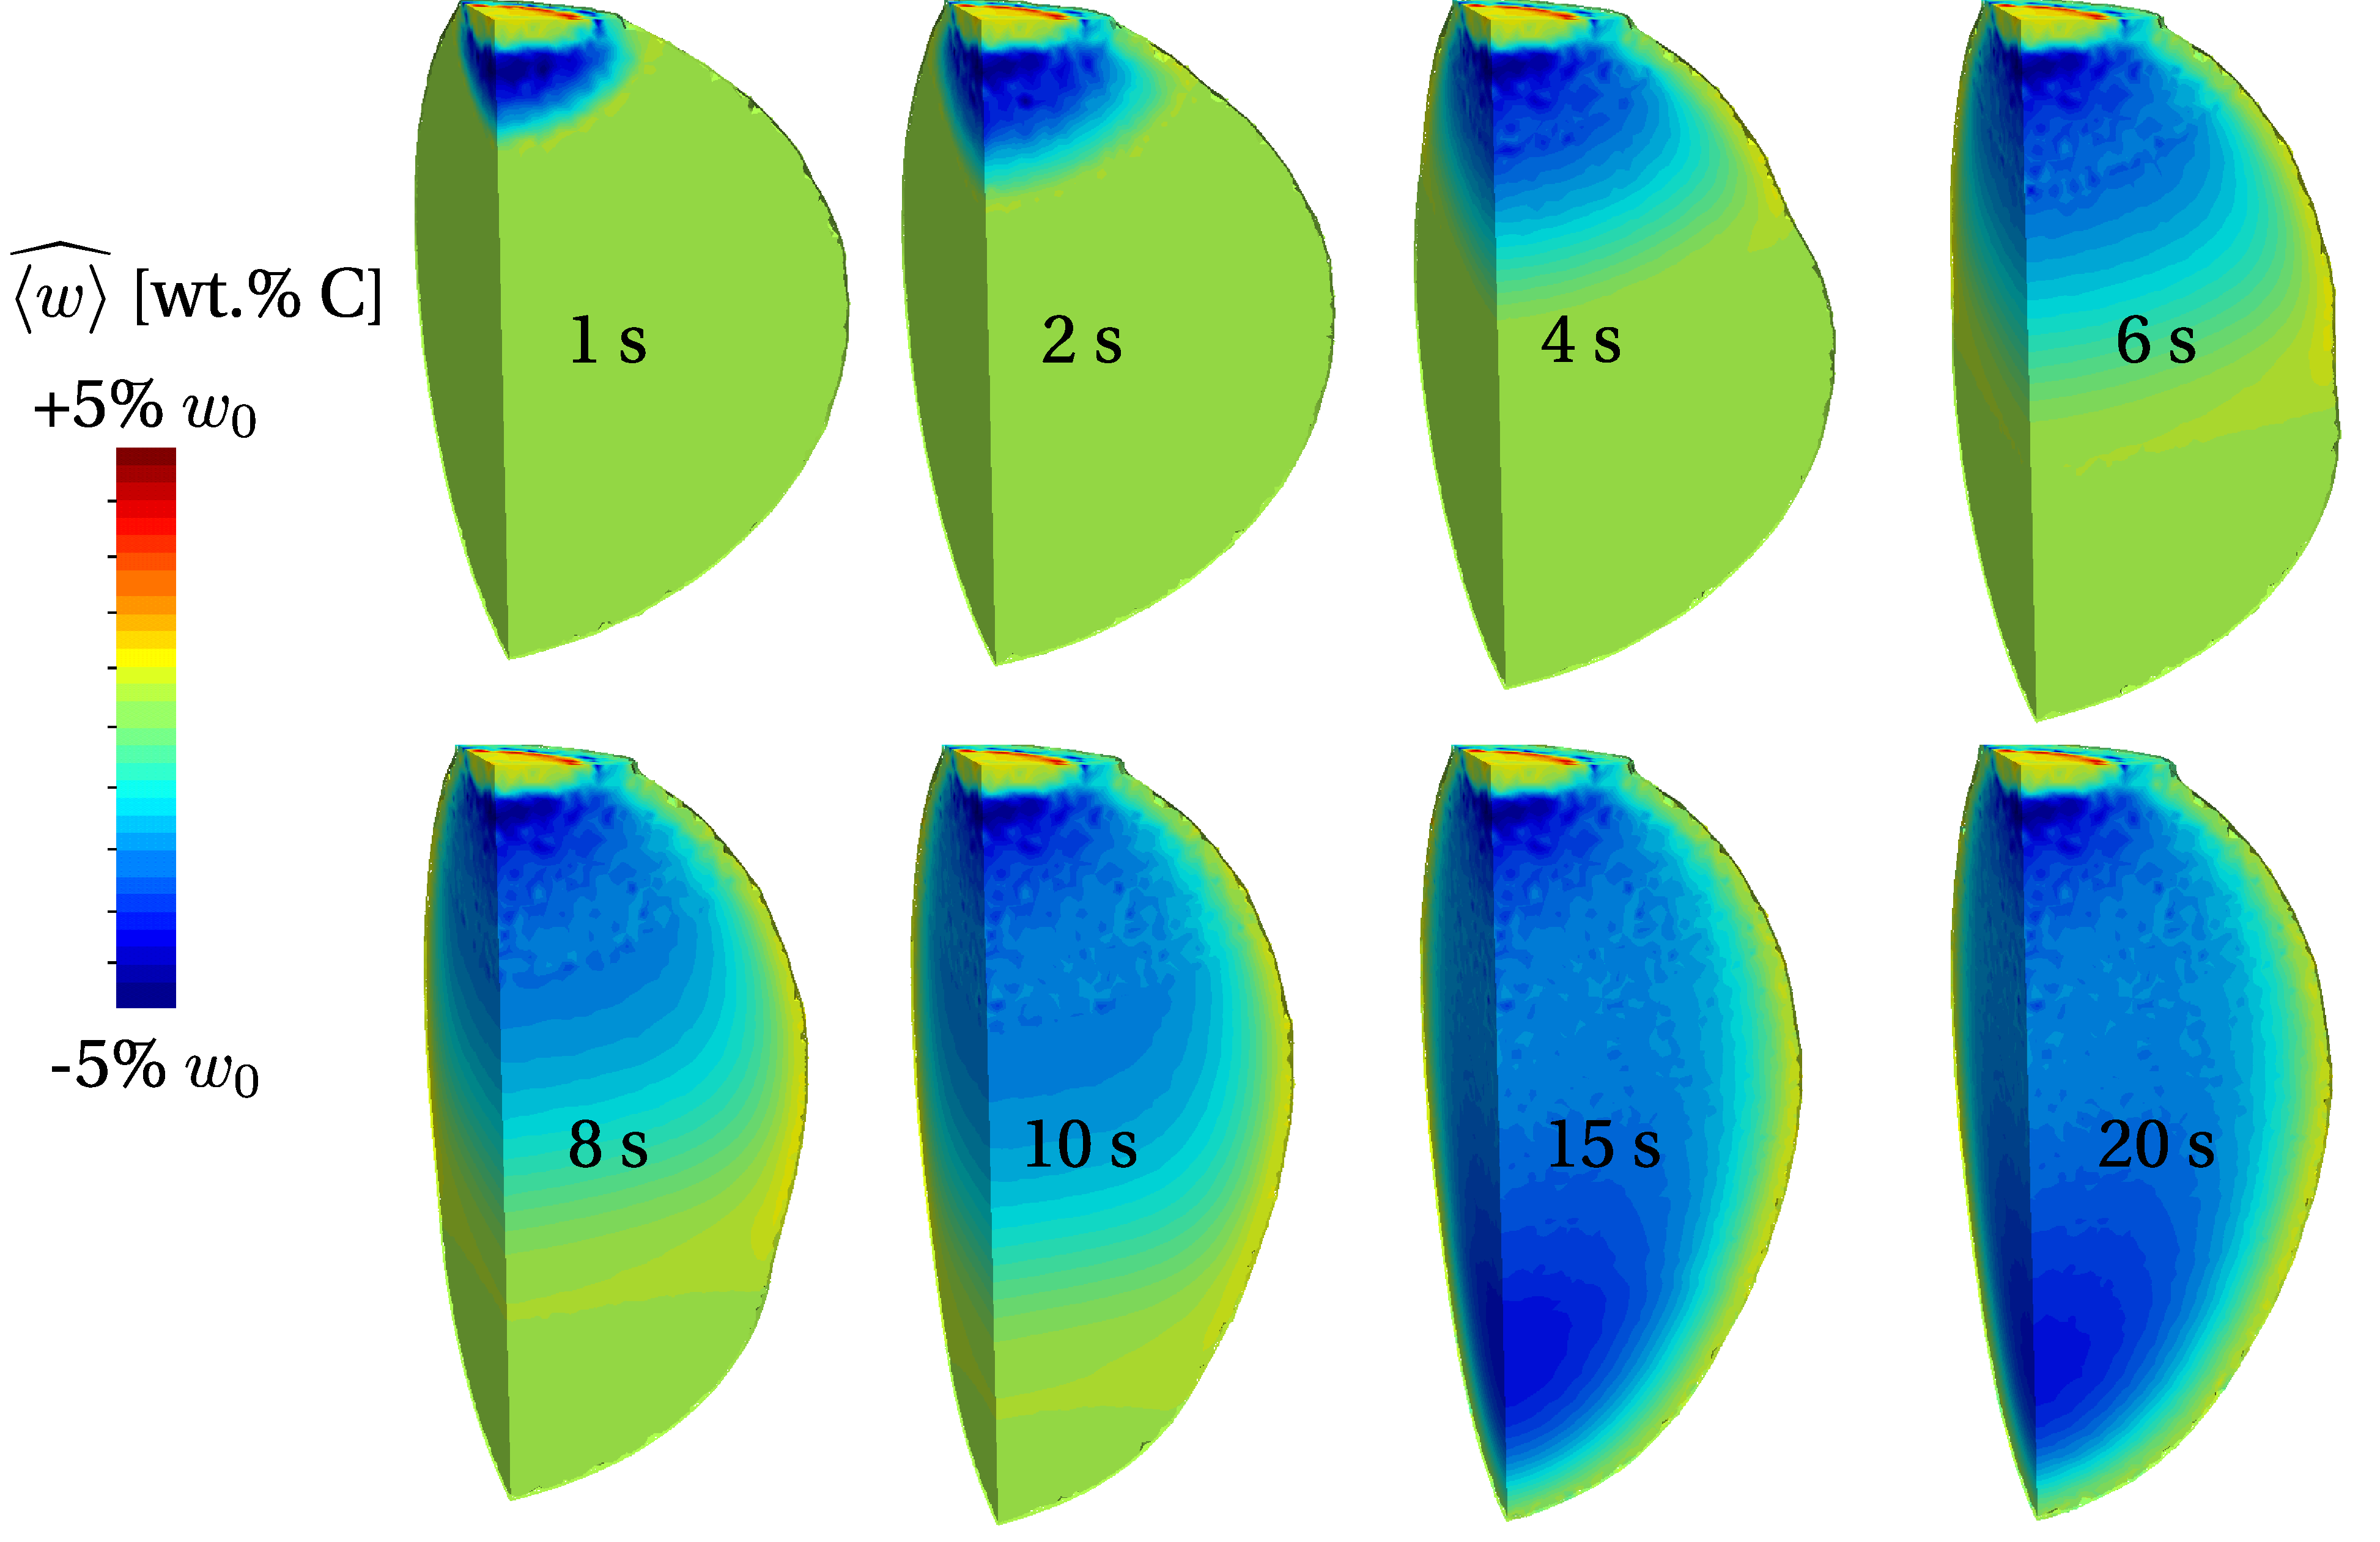
\includegraphics[width=1.0\textwidth]{Chapter5/Graphics/3d/bin/mesosegregation.pdf}
    \caption{Evolution of the average composition with solidification time, showing evidence of segregation and shape deformation between 0 s and 20 s.
     (check animation in the PDF file).} 
    %-------
  }
\label{fig:texus_mesosegregation}
\end{figure}
%===================================== ANIMATION FIGURE =====================================

%--------------------------------------
\shorthandoff{;:?!} %http://tex.stackexchange.com/questions/74860/unexpected-clash-between-babel-and-pgf-spy
\begin{figure}[htbp]
\centering
%-------
\begin{tikzpicture}%[spy using outlines={rectangle, magnification=3, width=1cm, height=6cm, connect spies}]
%[spy using outlines={circle, magnification=3, connect spies}]
%-------------------
 \begin{axis}
  [	name=whatever,
	%title= (c),
	scale only axis,
	table/col sep=comma,  % comma % tab
	enlarge x limits=false,
	%legend pos=north east,
	scaled ticks=true,
	ylabel style={align=center},
	ylabel=  Relative content $\frac{\avg{w}-w_0}{w_0}$ (\%), %Relative mesosegregation,
	xlabel=Distance from chill (mm),
	%xticklabel style={/pgf/number format/fixed},
	yticklabel style={/pgf/number format/fixed},
	xtick={0,1,...,8},
	xticklabels={0,1,...,8},
	ytick={-5,-2.5,...,5},
	yticklabels={-5,-2.5,...,5},
	%x tick label style={rotate=45,anchor=east},
	width=0.85\textwidth,
	height=8cm,	
	ymin=-5, ymax=5,
	xmin=0, xmax=8,
	mark repeat	= {50},
	%cycle list name=mycycle, %exotic,
	axis y line*=left,
]
  \addplot table [x expr=1000*\thisrow{arc_length}, y expr=100*(\thisrow{Concentration}-0.105)/0.105, color=red, mark=*]   {Chapter5/Data/3d_segregation/BinTransformationPath.csv};
	\draw[thick, dashed, black, opacity=0.5] (axis cs:\pgfkeysvalueof{/pgfplots/xmin},0.0) -- (axis cs:\pgfkeysvalueof{/pgfplots/xmax},0.0);
	\legend{$\avg{w}$}  	
  	\end{axis}
  	%-------------------
  	%-------------------
  	\begin{axis}
  [	name=whatever,
	%title= (c),
	scale only axis,
	table/col sep=comma,  % comma % tab
	scaled ticks=true,
	ylabel= Phase fraction (-),
	yticklabel style={/pgf/number format/fixed},
	%ytick={0,0.2,...,1},
	%yticklabels={0,0.2,...,1},
	width=0.85\textwidth,
	height=8cm,	
	ymin=0, ymax=1.05,
	xmin=0, xmax=8,
	mark repeat	= {50},
	cycle list name=mycycle,
	axis y line*=right,
	axis x line=none,
]
	\addplot table [x expr=\thisrow{arc_length}*1000, y=FractionBCC_c] {Chapter5/Data/3d_segregation/BinTransformationPath.csv};
	\addplot table [x expr=\thisrow{arc_length}*1000, y=FractionFCC_c] {Chapter5/Data/3d_segregation/BinTransformationPath.csv};
	\addplot table [x expr=\thisrow{arc_length}*1000, y=FractionCEM_c] {Chapter5/Data/3d_segregation/BinTransformationPath.csv};
	%\draw[thick, dashed, black, opacity=0.5] (axis cs:\pgfkeysvalueof{/pgfplots/xmin},0.0) -- (axis cs:\pgfkeysvalueof{/pgfplots/xmax},0.0);
	\legend{FCC,BCC,CEM}
  	\end{axis}
\end{tikzpicture}
%-------
\caption{Relative segregation profile in percent with respect to the nominal composition, 
along the vertical revolution axis of the solidified sample at a temperature lower than \SI{1100}{\udegC}.
Phase fractions are superimposed on the same graph and their values are read on the right y-axis.}
\label{fig:texus_segreg_profile}
\end{figure}
%--------------------------------------
\shorthandon{;:?!} %http://tex.stackexchange.com/questions/74860/unexpected-clash-between-babel-and-pgf-spy



A better global visualisation of the transformation is given in \cref{fig:texus_phase_distrib}, at different time stages.
Each column depicts a definite time with temperature and phase distribution. 


%--------------
\begin{figureth}
% textwidth 
{0.9}
%path 
{Chapter5/Graphics/3d/bin/phase_distrib.pdf}
% caption
{Solidification progress at 5, 10, 15 and 20 s showing the effect of segregation on the transformation paths, from liquid to solid and solid-state.}
% label
\label{fig:texus_phase_distrib}
\end{figureth}
%--------------


% ------------------------------------------------------
\subsection{Texus ternary and quaternary alloys}
% ------------------------------------------------------

In this section, the aim is to predict macrosegregation in reduced-gravity solidification of the \emph{b1} alloy, the latter being considered 
as a ternary and then as a quaternary alloy (cf. \cref{table:texus_b1}). 
%For simplicity, we refer to these alloys respectively by \emph{b1T} and \emph{b1Q}.
We want to show that, on the one hand our model handles multicomponent alloys (based on equilibrium conditions), while
on the other hand, how transformation paths vary by adding additional components, thus changing the shrinkage kinetics, hence the final sample shape.
%By introducing additional chemical species, silicon for \emph{b1Tern}, silicon and magnesium for \emph{b1Quat}, a new carbide phase may appear, the M$_7$C$_3$.
The first visible sign of different paths during solidification is given in \cref{fig:multicomp_liquid}. We can see that upon adding
additional chemical species while applying the same cooling conditions, a different liquid fraction remains after 15 s, showing evidence 
of slower solidification as we go from binary to quaternary. Also, with multicomponent alloys like \emph{b1Tern} and \emph{b1Quat}, an additional solid
phase may appear, that is the M$_7$C$_3$ carbide.
%After 15 seconds of chill contact, the \emph{b1Tern} and \emph{b1Quat} alloys have more volume fraction of liquid than \emph{b1Bin} computation as shown in 
%\cref{fig:multicomp_liquid}, meaning that solidification in these samples is slower. 
%The reason can be attributed to new solidification paths created by the more complex system composition compared  to the binary sample. 
% Slower solidification means that the final predicted shape is different, as shown earlier in the parametric study.
Slower cooling rates result in more elongated droplet shapes due to weight force, whereas shrinkage forces tend to counter this effect.
Therefore the final predicted shape is different, as shown earlier in the parametric study.

%--------------
\begin{figureth}
% textwidth 
{0.9}
%path 
{Chapter5/Graphics/3d/tern_quatern/gl15s.pdf}
% caption
{Snapshots showing the remaining volume fraction of liquid at 15 s in each sample of the binary, ternary and quaternary \emph{b1} alloy.}
% label
\label{fig:multicomp_liquid}
\end{figureth}
%--------------

In \cref{fig:shape_comparison}, we focus on the final droplet profile caused by varying the number of solute elements.
We clearly notice that the multicomponent solidification results in a slightly more elongated shape. 
All cases were obtained using the optimal simulation
parameters determined previously by the parametric study, i.e. thermal exchange coefficient, $\hext$, of \SI{6e4}{\uhconvec} and a gravitational
acceleration, $\norm{\gravity}$, of \SI{5e-5}{\uacceleration}. The clear difference in solidification paths requires to do the same 
parametric study to get better simulation-vs-experiment prediction. However, as we have shown earlier the effect of varying these parameters
on the final profile, we do not perform parametric studies for \emph{b1Tern} and \emph{b1Quat} alloys. 

The vertical elongation obtained by the \emph{b1Tern} sample is almost the double of the \emph{b1Bin} result. Moreover, the final ternary and quaternary
profiles are almost overlapping, indicating that the prediction accuracy is very close for these alloys. 
This reveals the importance of simulating solidification processes with real alloy compositions instead of binary simplifications
where the transformation path is not complex as a result of the smaller number of phases forming at equilibrium. 

%--------------
\begin{figureth}
% textwidth 
{0.9}
%path 
{Chapter5/Graphics/3d/tern_quatern/profiles_comparison.pdf}
% caption
{Comparison of final droplet profiles obtained by solidifying \emph{b1Bin}, \emph{b1Tern} and \emph{b1Quat} samples, with respect to the initial profile. 
The \emph{b1BinCoarse} sample
is obtained using coarser composition steps.}
% label
\label{fig:shape_comparison}
\end{figureth}
%--------------

Nevertheless, it should be mentioned that the mapping resolution plays an important role in the accuracy of thermodynamic conversions.
Therefore, tabulations size easily increases with the increasing number of solute elements, because of the greater number of temperature-composition 
combinations to scan while computing equilibrium. To test the effect of changing the mapping resolution, we repeated the binary sample solidification
but with a composition step of \SI{0.0495}{\ucomposition} instead of \SI{0.0052}{\ucomposition} used for the \emph{b1Bin} sample, i.e. about 10 times coarser. 
The corresponding profile in \cref{fig:shape_comparison}, \emph{b1BinCoarse}, shows less vertical elongation then predicted by the finer \emph{b1Bin} tabulation. 
This is clearly due to inaccurate calculation of the solidification path, revealing the importance of mappings accuracy in predicting transformation-related physics.

In order to test the effect of the tabulation file size on computation time, we simulate again the quaternary solidification case but this time with a lightweight
tabulation where all successive line with similar phase fractions outside the solidification range are deleted, giving what we call \emph{b1QuatLite}. The 
resulting file is three time smaller than the original tabulation file. Surprisingly, the computation time for \emph{b1QuatLite} shows no significant acceleration 
compared to \emph{b1Quat}. The file size, proportional to the number of tabulated lines, is important as it causes a search overhead each time the conversion module
is called. However, \cref{table:mapping_stat} reveals that the multi-variable interpolation overhead is even more important, resulting in longer computation times.
This may be considered as a limitation of the thermodynamic mapping approach.

%is another cause of the shape discrepancy, and the thermodynamic mapping
% of the binary alloy has the advantage: less solute elements means less 
% It becomes then clear that a multicomponent mapping has a greater number of combinations to scan in order to get the corresponding transformation paths, compared
% to a binary mapping. For that reason, the multicomponent mapping is often coarser than the binary one to limit the search and interpolations overhead, 
% leading to smaller tabulation files but less accurate path prediction. This is may be considered as a limitation of the thermodynamic mapping approach.


%--------------------------------
\begin{table}[htbp]
\centering
\caption{Information table showing the tabulations size  for each alloy obtained by the same mapping resolution for temperature and composition, 
depending on the number of solute elements and phases. The temperature step is \SI{1}{\udegC} and the range is the range is [\SI{20}{\udegC}-\SI{1620}{\udegC}] for all four cases . 
The computation time corresponds to the CPU time of a simulation running on 20 cores.}
\label{table:mapping_stat}
\resizebox{\columnwidth}{!}{%
{\tabulinesep=1.0mm \begin{tabu}{lccccccc}
\tabucline[1pt]{-}
\textbf{Alloy} & \textbf{Nb solutes} &  \textbf{Composition range (\si{\ucomposition})}  & \textbf{Composition step (\si{\ucomposition})}  & \textbf{Nb phases}  
& \textbf{Tabulation lines}  & \textbf{Size (MB)} & \textbf{Computation time (s)}  \\\tabucline[1pt]{-}
%-----------------------------
      \emph{b1Bin}  	& 1 &	C: [0.0945-0.1155] &   0.00525  &  4 &  \num{185010} &    \num{4.37}   &  \num{59461.5}  \\   %78003.9
      \emph{b1Tern} 	& 2 &	C: [0.0945-0.1155] &   0.00525  &  5 &  \num{220250} &    \num{10.18}  &  \num{62644.4}  \\    
      					&   &  Si: [0.2412-0.2948] &   0.0134   &    &               &                 &                 \\    
      \emph{b1Quat} 	& 3 &	C: [0.0945-0.1155] &   0.00525	&  5 &  \num{1101250}&    \num{66.89}  &  \num{85476.7}  \\     
      					&   &  Mn: [0.5724-0.6996] &   0.0318   &    &               &                 &                 \\    
      					&   &  Si: [0.2412-0.2948] &   0.0134   &    &               &                 &                 \\    
      \emph{b1QuatLite} & 3 & 	C: [0.0945-0.1155] &   0.00525	&  5 &  \num{326014} &    \num{20.93}  &  \num{84104.8}  \\
      					&   &  Mn: [0.5724-0.6996] &   0.0318   &    &               &                 &                 \\    
      					&   &  Si: [0.2412-0.2948] &   0.0134   &    &               &                 &                 \\\tabucline[1pt]{-}
      % http://grammarist.com/words/lite/
%-----------------------------
\end{tabu}}
}
\end{table}
%--------------------------------

Finally we are interested in comparing the macrosegregation levels obtained in all three solidification cases. Segregation maps
are presented in \cref{fig:final_segreg_ternquat} on a symmetry plane section. First, we compare the carbon segregation as it is the common species among the presented alloys.
The first difference is a remarkable positive macrosegregation of 3.5\% at the chill contact of the  \emph{b1Tern} and \emph{b1Quat} samples, 
while being less prominent for \emph{b1Bin} which shows a relative segregation of 1.2\%. As we explained earlier, this positive macrosegregation taking place at the beginning
of solidification is related to the shrinkage flow (cf. \cref{fig:texus_flow}) created by the strong thermal gradient in the contact zone. 
As the thermal gradient in this zone is almost the same
for all three cases at solidification onset, the higher velocity which is responsible for the noticeable positive macrosegregation in both multicomponent samples,
is related to the solidification path varying with the number of species.
Two regions of negative macrosegregation are observed across the samples, with various amplitudes. The first region lies just below the positive segregation contact surface.
It corresponds to the solute depletion caused by an upward shrinkage flow and a downward gravity flow. With the advancement of the solidification front,
the gravity flow dominates creating a radial outward negative segregation pattern where  


%--------------
\begin{figureth}
% textwidth 
{1.0}
%path 
{Chapter5/Graphics/3d/tern_quatern/final_segreg.pdf}
% caption
{Segregation maps relative to each alloy, showing positive and negative mesosegregations 
of each chemical species for \emph{b1Bin}, \emph{b1Tern} and \emph{b1Quat} samples.}
% label
\label{fig:final_segreg_ternquat}
\end{figureth}
%--------------



%--------------------------------------
\shorthandoff{;:?!} %http://tex.stackexchange.com/questions/74860/unexpected-clash-between-babel-and-pgf-spy
\begin{figure}[htbp]
\centering
%-------
\begin{tikzpicture}%[spy using outlines={rectangle, magnification=3, width=1cm, height=6cm, connect spies}]
%[spy using outlines={circle, magnification=3, connect spies}]
  \begin{axis}
  [ name=one,
  title= (a) carbon segregation,
  %at=(one.right of south east), anchor=left of south west,
  scale only axis,
  table/col sep=comma,  % comma % tab
  enlarge x limits=false,
  %legend pos=north east,
  scaled ticks=true,
  %xlabel=Sample length (m),
  ylabel=$\frac{\avg{w_C}-w_{C_0}}{w_{C_0}}$ (\%),
  % xticklabel style={/pgf/number format/fixed},
  xtick={0,1,...,8}, 
  xticklabels={},
  ytick={-5,-2.5,...,5},
  %x tick label style={rotate=45,anchor=east},
  width=0.9\textwidth,
  height=5cm, 
  ymin=-5, ymax=5,
  %xmax=0.0928,
  mark repeat = {100},
  cycle list name=mycycle, %exotic,
  ]

  \addplot table [x expr=1000*\thisrow{arc_length}, y expr=100*(\thisrow{Concentration}-0.105)/0.105]   {Chapter5/Data/3d_segregation/centersegreg_bin.csv};
  \addplot table [x expr=1000*\thisrow{arc_length}, y expr=100*(\thisrow{Concentration_C}-0.105)/0.105] {Chapter5/Data/3d_segregation/centersegreg_tern.csv};
  \addplot table [x expr=1000*\thisrow{arc_length}, y expr=100*(\thisrow{Concentration_C}-0.105)/0.105] {Chapter5/Data/3d_segregation/centersegreg_quat.csv};
  \legend{\emph{b1Bin}, \emph{b1Tern}, \emph{b1Quat}}
  \end{axis}
%-------------------
 \begin{axis}
  [ name=two,
  title= (b) silicon segregation,
  at=(one.below south west), anchor=above north west,
  scale only axis,
  table/col sep=comma,  % comma % tab
  enlarge x limits=false,
  %legend pos=north east,
  scaled ticks=true,
  %xlabel=Sample length (m),
  ylabel=$\frac{\avg{w_{Si}}-w_{{Si}_0}}{w_{{Si}_0}}$ (\%),
  xticklabel style={/pgf/number format/fixed},
  xtick={0,1,...,8}, 
  xticklabels={},
  ytick={-1,-0.5,...,1},
  %x tick label style={rotate=45,anchor=east},
  width=0.9\textwidth,
  height=5cm, 
  ymin=-1, ymax=1,
  %xmax=0.0928,
  mark repeat = {100},
  cycle list name=mycycle,
  ]
  \addplot table [x expr=1000*\thisrow{arc_length}, y expr=100*(\thisrow{Concentration_Si}-0.268)/0.268] {Chapter5/Data/3d_segregation/centersegreg_tern.csv};
  \addplot table [x expr=1000*\thisrow{arc_length}, y expr=100*(\thisrow{Concentration_Si}-0.268)/0.268] {Chapter5/Data/3d_segregation/centersegreg_quat.csv};
  \legend{\emph{b1Tern}, \emph{b1Quat}}
  \end{axis}
%-------------------
 \begin{axis}
  [ name=three,
  title= (c) manganese segregation,
  at=(two.below south west), anchor=above north west,
  scale only axis,
  table/col sep=comma,  % comma % tab
  enlarge x limits=false,
  %legend pos=north east,
  scaled ticks=true,
  xlabel=Distance from chill (mm),
  ylabel=$\frac{\avg{w_{Mn}}-w_{{Mn}_0}}{w_{{Mn}_0}}$ (\%),
  xtick={0,1,...,8}, 
  xticklabels={0,1,...,8}, % showing in (mm)
  ytick={-1,-0.5,...,1},
  % xticklabel style={/pgf/number format/fixed},
  width=0.9\textwidth,
  height=5cm, 
  ymin=-1, ymax=1,
  mark repeat = {100},
  cycle list name=mycycle, %exotic,
  ]
  \addplot table [x expr=1000*\thisrow{arc_length}, y expr=100*(\thisrow{Concentration_Mn}-0.636)/0.636] {Chapter5/Data/3d_segregation/centersegreg_quat.csv};
  \legend{\emph{b1Quat}} 
  \end{axis}

\end{tikzpicture}
%-------
\caption{Relative macrosegregation profiles as functions of the distance from the chill, plotted for (a) carbon (b) silicon and (c) manganese elements
along the vertical revolution axis of the solidified sample.}
\label{fig:3d_segregation_multicomponent}
\end{figure}
%--------------------------------------
\shorthandon{;:?!} %http://tex.stackexchange.com/questions/74860/unexpected-clash-between-babel-and-pgf-spy

% \comment{update binary profile comparison as well as the corresponding image}
% \comment{update parametric study H3G0 and H4G0 given by new tabulation}
% \comment{introduce and comment the tabulation resolution and its effect on shape}
%\comment{update the binary 1d segregation anaysis at the end in the bin tern quat comparison}
%\comment{update computation time for ternary done with 20 cores}
%\comment{update solidification progress figures for phase fractions with the binary solidification obtained with the finer tabulation}
 
%--
\clearpage
\section*{Résumé chapitre 5}

\begin{otherlanguage}{french}
{\small

Ce dernier chapitre est dédié à la prise en compte du retrait à la solidification à l'origine de la 
déformation de la surface libre métal-air, en présence des phénomènes de ségregation.
Pour ce faire, le modèle de solidification utilisé précédemment pour prédire la macroségrégation induite 
par convection thermosolutale en monodomaine, est enrichi par une méthode de suivi direct d'interface, la level set. %, déjà introduite dans le chapitre 2. 
Les équations du modèle sont alors reformulées dans un contexte 
eulérien multidomaine-multiphase, i.e. où deux domaines mutliphasés sont séparés
par une interface mobile, l'aspect mutliphase dans chaque domaine étant géré par la méthode de prise de moyenne volumique. 


Un premier cas d'application 1D est ensuite présenté. C'est un cas qui avait fait l'ojet de validation du \emph{Tsolver} dans le chapitre 3,
et qui est refait avec des masses volumiques solide et liquide différentes. Cette application simple permet toutefois de comprendre le phénomène
de ségrégation inverse résultant de l'écoulement du liquide vers le front de solidification pour compenser la différence
des masses volumiques des phases, ce qui enrichit en solutés la partie du métal en contact avec le refroidisseur. 
Ce phénomène est souvent observé en surfaces des lingots en contact avec les moules. Des courbes de refroidissement ainsi qu'un bilan de conservation de masse de métal sont
présentés pour permettre de comprendre l'effet de l'introduction de la méthode level set sur la physique de la solidification.


La seconde application est aussi un cas de validation utilisé dans un chapitre précédent, issu d'une simulation sans retrait présente dans la litérature \citep{carozzani_direct_2013}.
Cependant, le but en est maintenant de tester la robustesse du modèle
en présence de convection naturelle, d'origine thermique dans l'air et thermosolutale dans le métal, avec suivi de déformation de l'interface par retrait à la solidification.
Nous utilisons une méthode de remaillage adaptatif basée sur la projection sur les arêtes \citep{coupez_solution_2013}, 
permettant d'avoir une résolution de maillage fine autour des zones d'intérêt, notamment l'interface décrite par level set, le vecteur vitesse
et la concentration moyenne. Ce couplage de techniques numériques permet de déterminer à la fois la retassure en surface du lingot et la macroségregation,
présente également sous forme de canaux.


Dans le dernier cas, il s'agit de la solidification d'une goutte d'acier en microgravité. 
Des essais expérimentaux de solidification déclenchée par contact avec un substrat sont présentés avec la forme finale de la goutte.
Pour pouvoir prédire la déformation de la goutte en présence de ségrégations, nous considérons trois nuances issues du même alliage:
un binaire (\emph{b1Bin}) Fe-C, un ternaire (\emph{b1Tern}) Fe-C-Si et finalement un quaternaire (\emph{b1Quat}) Fe-C-Mn-Si.
D'abord, une étude paramétrique est faite en se servant de l'alliage binaire, dans le but de déterminer les paramètres optimaux de vitesse
de refroidissement et d'accélération gravitationnelle, pour se rapprocher du profil expérimental de la goutte déformée en fin de solidification.
Ensuite, nous simulons la solidification de chaque alliage en montrant la déformation finale ainsi que la distribution finale
des espèces chimiques.  

}
\end{otherlanguage}
 % resume francais


 % Application to TEXUS

\chapter*{Conclusion and Perspectives}
\addstarredchapter{Conclusion and Perspectives}

%\minitoc
%\newpage

% \section*{Conclusions}
The current thesis proposes a numerical model to predict macrosegregation in different contexts: without or
with overall metal volume change. The first case considers no average density change during solidification, 
assuming that the liquid and solid phases in the metal have the same density. 
On the other hand, the second case considers that the difference in metallic phase densities causes the average density to change, causing the metal's volume to
change concurrently. 

\paragraph{Temperature resolutionT compatible with thermodynamic mapping:}
In this thesis, we have introduced and validated a finite element method to solve energy conservation with phase change, based 
on thermodynamic data mapping and having the temperature as a main variable (\emph{Tsolver}). The algorithm proved to be faster for several computations
shown in chapters 3 and 4, when compared to the enthalpy-based method (\emph{Hsolver}). The approach is also well suited to predict macrosegregation
of both binary and multicomponent alloys. Some limitations are met nevertheless. It is important to have prior knowledge of composition variations
during solidification in order to adapt to limit the mapping size while also keeping fine composition and temperature steps.
Finer steps ensure more accurate transformation paths. We may also conclude that this thermodynamic mapping approach is still
to equilibrium assumptions (full equilibrium or solid-liquid interface equilibrium). \citet{tourret_multiple_2011} proposed
a similar solution but supports more than just a lever rule for microsegregation, by allowing input of diffusion coefficients.

\paragraph{Channel segregation:}
Using our energy solver, the Navier-Stokes solver and species conservation solver, we attempted modelling an experimental benchmark 
of directional (upward) \bin{In}{75}{Ga} solidification. Some of the experimental data was used to a get a closer numerical configuration to the experiment.
Two scales of modelling were considered, a purely macroscopic finite-element (FE) approach and a coupled mesoscopic-macroscopic approach
relying on cellular automata (CA) for the small scales and also on FE for the greater scales, hence the approach name CAFE. 
The pure FE model considers only average macroscopic conservation equations (mass, energy, species and liquid momentum) 
on a finite-element grid, with a constant volume for the metal, i.e. no shrinkage is possible. 
The FE approach resulted in either no channel segregation at all at low temperature gradients, or a limited number of channels when
the temperature gradient was increased. These numerical observations reveal however discrepancy in the general fluid flow behaviour and 
subsequent formation of segregation channels, when qualitatively compared to experimental findings.
This is where the CAFE model is introduced to show the advantage of nurturing the FE scale with feedback information coming from
the lower scale CA grid, where nucleation and growth of grain envelopes are systematically solved.
Indeed, CAFE predictions showed a noticeable difference with respect to the pure FE approach. The overall fluid flow pattern is 
much more complicated and random, many convective plumes form mainly at grain boundaries as a result of solute enrichment inside the mushy zone (solutal convection),
powered also by the temperature gradient (thermal convection).   
The comparison between the experimental data and numerical predictions is only qualitative, due to the lack of an array of crucial data, such 
as the nuclei positions, the undercooling, magnitude of fluid flow inside the rising convective plumes and others.
In order to conduct a quantitative comparison, such data may be very useful to calibrate the CAFE model.
The second limitation in this comparison is the difficulty of simulating the real solidification cell with a thickness of \SI{150}{\micro \metre}.
Therefore, the simulations considered an alternate thickness of \SI{1}{\milli \metre}, due to the huge FE mesh that would be obtained if
we want at least 5 elements in the thickness to correctly predict the flow. Using adaptive remeshing could be a solution, but should be used
with care since small elements are almost needed everywhere in the mushy zone where thermosolutal convection is initiated.   
It is interesting to model the entire thin solidification cell for future research. In addition, it is interesting to compare simulation
results with real single grain casting experiments, which allow to understand better the basic mechanisms of channel segregation, which
could precede the formation of freckle defects.

\paragraph{Solidification shrinkage:}
To model this phenomenon, we go from the previous FE model, and reformulate the conservation equations to be compatible with the level set method,
which helps us track the boundary between the metal and a surrounding gas domain. The presence of the latter is important as its volume should compensate
for the metal's volume shrinkage. A detailed analysis is given to explain the various interfaces which form the metal-air boundary in reality along
with the necessary assumptions to get the equivalent definition in the model.
The monolithic energy, fluid momentum and species conservation equations incorporate the volume change in the metal by using the mass balance.
A modified Darcy was defined to account for the presence of the gas domain in the monolithic fluid momentum equation.
Regarding species conservation, three modelling strategies were introduced: if we consider that the gas domain contains fictitious metallic species, 
then we may define a monolithic strategy with limited solute diffusion known as MD, and a monolithic strategy with limited diffusion and advection in the gas known as MDA.
The third strategy consists of solving for species conservation in the metal while completely disregarding the gas domain, then making the necessary correction. 
\newline
\newline
Three applications cases are presented in the increasing order of modelling dimension: 1D, 2D and 3D. The first application shows the performance of the model
applied to one-dimensional solidification shrinkage configuration without then with macrosegregation, using each of the 3 proposed strategies.
The results show an instability in the predicted average composition field surrounding the metal-air boundary, where a positive segregation peak is
seen in the air domain. This peak amplitude is reduced when the MDA strategy is used, and almost disappears with the NM strategy. A full analysis 
made for each strategy reveals that the latter species conservation strategy performs better than the former two, without having a bad effect
on species mass conservation and metal mass conservation.
\newline
\newline
The 2D application is based on a comparison with a \bin{Sn}{3}{Pb} solidification benchmark that 
simulates the configuration of \citet{hebditch_observations_1974} experiments. The experiment
was simulated by \citet{carozzani_direct_2013} assuming a constant volume for the metal. In this work, the level set context allows predicting
the final ingot shape once completely solidified. The added value of this result with respect to previous
simulation attempts is the prediction of mesosegregation and macrosegregation trends in the shrunk ingot, which is closer to the experimental results.
As future work, it may be interesting to couple the work done by \citet{chen_3d_2014} for grain structure prediction
in an increasing metal volume using the level set context with the current developments in order to get more
accurate predictions compared to the experiment. Knowing that all the previous suggestions are made in the context
of a fixed and rigid solid phase, it is also interesting to continue research in the direction of coupling the
fluid and solid mechanics in the same simulation.
\newline
\newline
The 3D application simulates solidification of a small steel droplet in a reduced-gravity environment, as
an extension to the work of \citet{rivaux_simulation_2011}. A parametric study is performed to determine
the best heat transfer coefficient values of the contact surface with the ceramic chill, and the magnitude of the microgravity vector
resulting.The optimal values were used to simulate solidification of the steel droplet, but approximating the composition by a binary equivalent.
Segregation and subsequent phase distributions analysis is given. Later, the same simulation is conducted but considering
ternary and quaternary approximations of the steel. Segregation profiles do not high segregation intensities due to the limited flow under
reduced gravity. An analysis of the competition of fluid motion between microgravity forces and suction to shrinkage inside the droplet is given.   







% \section*{Future Work}
% \comment{What did we miss in our models that can be potentially important for the coming years} % Conclusion

% ********************************** Appendices ********************************
%\appendixpage
\begin{appendices} % Using appendices environment for more functunality
\chapter{Notes}

from \url{http://aerojet.engr.ucdavis.edu/fluenthelp/html/ug/node572.htm} \\

For many natural-convection flows, you can get faster convergence with the Boussinesq model than 
you can get by setting up the problem with fluid density as a function of temperature. This model 
treats density as a constant value in all solved equations, except for the buoyancy term in the momentum 
equation:
\begin{align}
 (\rho - \rho_0) g \approx -\rho_0 \beta (T - T_0) g 	
\end{align}

where  $\rho_0$ is the (constant) density of the flow,  $T_0$ is the operating temperature, and  $\beta$ is 
the thermal expansion coefficient. Equation  13.2-18 is obtained by using the Boussinesq approximation  
$\rho = \rho_0 (1 - \beta \Delta T)$ to eliminate  $\rho$ from the buoyancy term. This approximation is accurate as 
long as changes in actual density are small; specifically, the Boussinesq approximation is valid when  $\beta(T-T_0)\ll 1$.
\chapter{Resolution algorithm with LSM}



\newcommand{\vI}{\textbf{v}_{\text{I}}  }
\newcommand{\vII}{\textbf{v}_{\text{II}}  }
\newcommand{\capt}{\;\mathrm{capt}}
\newcommand{\deriv}[1]{\frac{\partial #1 }{\partial t}}
\newcommand{\diff}[2]{ \ensuremath{\nabvec \cdot\left( #1 \nabvec #2 \right)  }}
% This command is useful to have quick control over the format of all header titles
\newcommand{\name}[1]{\textbf{#1}}


\begin{figure}
\newlength{\largeur}
\newlength{\llargeur}
\newlength{\rlargeur}

\setlength{\largeur}{4.5cm}
\setlength{\llargeur}{10.8cm}
\centering
\begin{tikzpicture}[node distance=0.4cm]

\tikzstyle{rect}=[rectangle,draw,text=black, fill=red!10, drop shadow, rounded corners]
\tikzstyle{test}=[diamond,aspect=3,draw,text=black]
\tikzstyle{fleche}=[->,>=stealth]
\tikzstyle{trait}=[]

\setlength{\rlargeur}{\largeur}
\addtolength{\rlargeur}{-1.\tabcolsep}
\addtolength{\rlargeur}{-1.\llargeur}

\node[rect] (comment) at (0,7)
{
	$\avg{H}^t$, $T^t$, $g^{\phi}_j$, $(dH/dT)^t_j$ 		
};

\node[rect,below=of comment] (mecaflu)
{
	\begin{tabular}{@{}p{\llargeur}p{\rlargeur}@{}}
	\name{Mechanics Step II : Fluid-oriented Resolution}
	\begin{equation*}
	  \begin{array}{l l}
	    %{\rho}^{l}_{\text{ref}} 
		%\brac{\frac{\partial \brac{g^{l} \vII }}{\partial t} + 
		% \nabvec \cdot\brac{g^{l} \vII  \times \vII  }} = \nabvec\cdot \brac{g^{l}\mathbb{S}^{l}} 
		%-  g^{l} \nabvec p^{l} + g^{l} {\rho}^{l} \vec{\mathbb{G}} - {g^{l}}^{2} \mu^{l} \mathbb{K}^{-1} \brac{ \vII  - \vI  } } \\ 
	    \nabvec \cdot \vII = 0
	  \end{array} 	
	\end{equation*}
	\end{tabular}
};


\node[rect,below=of mecaflu] (energy)
{
	\begin{tabular}{@{}p{\llargeur}p{\rlargeur}@{}}
	\name{Conservation of energy (Nonlinear Heat Transfer)} 
	\begin{equation*}
		\frac{\partial \avg{\rho h} }{\partial t} + 
		\avg{\vII} \cdot \nabvec \avg{\rho h}^{l}= 
		\diff{\avg{\kappa}}{T}
	\end{equation*}
	\end{tabular}
};


\node[rect,below=of energy] (macroseg)
{
	\begin{tabular}{@{}p{\llargeur}p{\rlargeur}@{}}
	\name{Conservation of chemical species (Macrosegregation)} 
	\begin{equation*}
		\frac{\partial \langle w_i \rangle}{\partial t} + 	
		\avg{\vII}  \cdot   \nabvec \langle w_i \rangle^{l} = 
		\nabvec\cdot  ( \langle D^{l} \rangle \nabvec \langle w_i \rangle^{l} )
	\end{equation*}
	\end{tabular}
};

\node[rect,below=of macroseg] (microseg)
{
	\begin{tabular}{@{}p{\llargeur}p{\rlargeur}@{}}
	\name{Microsegregation} 
	\begin{equation*}	   
	  \begin{array}{l l}
	    \brac{g^{\phi} , \avg{w_i^{\phi}}^{\phi} } = f\brac{\avg{w_i} , T }  \\ 
	    \frac{\partial \avg{\rho h} }{\partial T} = 
		 \frac{\partial}{\partial T} \brac{\sum_{\phi} g^{\phi}  \avg{\rho h}^{\phi} }
	  \end{array} 	
	\end{equation*}
	\end{tabular}
};

	
%\node[rect,below=of mecasol] (fe_calc)
%{
%	\begin{tabular}{@{}p{\llargeur}p{\rlargeur}@{}}
%		FE calculation & $\prescript{(k+1)}{}{\avg{H}}$ \\
%	\end{tabular}
%};
%
%\node[rect,below=of fe_calc] (init_micro)
%{
%	\begin{tabular}{@{}p{\llargeur}p{\rlargeur}@{}}
%		Micro time initialization & $t_m = t$ \\
%		Nodes initialization & $\avg{H}^{t_m} = \avg{H}^{t}$, $T^{t_m} = T^{t}$, $g^{s^{(j)}_i t_m} = g^{s^{(j)}_i t}$ \\
%		Cells initialization & $I^{(i) t_m}_\nu = I^{(i) t}_\nu$, $r^{(i) t_m}_\nu = r^{(i) t}_\nu$ \\
%	\end{tabular}
%};
%	
%\node[rect,below=of init_micro] (microt)
%{
%	\begin{tabular}{@{}p{\llargeur}p{\rlargeur}@{}}
%		Micro time step calc. & $\delta t = l_{CA} / v^{s_i}_{\nu \max}$ \\
%	\end{tabular}
%};
%	
%\node[rect,below=of microt] (init_cell)
%{
%	\begin{tabular}{@{}p{\llargeur}p{\rlargeur}@{}}
%		Cells initialization & $I^{(i)}_\nu = I^{(i) t_m}_\nu$, $r^{(i)}_\nu = r^{(i) t_m}_\nu$, $T^{t_m}_\nu = \sum_n \phi (x_\nu) T^{t_m}$ \\
%	\end{tabular}
%};
%
%\setlength{\rlargeur}{\largeur}
%\addtolength{\rlargeur}{-4.\tabcolsep}
%\addtolength{\rlargeur}{-6.5cm}
%
%\node[rect,below=of init_cell] (cells)
%{
%	\begin{tabular}{@{}p{2.cm}p{4.5cm}p{\rlargeur}@{}}
%		\textbf{Procedure} & \textbf{Tests} & \textbf{Modified variables at cells} \\
%		\textbf{Nucleation} & $I^{(i)}_\nu = 0$, $T_\nu < T^{s_i}_{nucl}$ & $I^{(i)}_\nu$, $r^{(i)}_\nu$, $V^{(i)}_{\nu \capt}$, $V^{(i)}_{\nu \max}$ \\
%		\textbf{Growth} & $I^{(i)}_\nu \not = 0$, $g^{(i)}_\nu < 1$, $T_\nu < T^{s_i}_{eq}$ & $r^{(i)}_\nu$ \\
%		\textbf{Capture} & $I^{(i)}_\nu = 0$, $T_\nu < T^{s_i}_{eq}$ & $I^{(i)}_\nu$, $r^{(i)}_\nu$, $V^{(i)}_{\nu \capt}$, $V^{(i)}_{\nu \max}$ \\
%	\end{tabular}
%};
%
%\setlength{\rlargeur}{\largeur}
%\addtolength{\rlargeur}{-2.\tabcolsep}
%\addtolength{\rlargeur}{-1.\llargeur}
%
%\node[rect,below=of cells] (fe)
%{
%	\begin{tabular}{@{}p{\llargeur}p{\rlargeur}@{}}
%		& \textbf{Modified variables at nodes} \\
%		\textbf{Retrocession} & $g^{(i) t_m+\delta t} = \sum_\nu \phi(x_\nu)g^{(i) t_m+\delta t}_\nu / \sum_\nu \phi(x_\nu)$ \\
%	%	\textbf{Enthalpy conversion} & $\avg{H}^{t_m + \delta t} = \avg{H}^{t} + (\prescript{(k+1)}{}{\avg{H}} - \avg{H}^{t}) \frac{t_m+ \delta t - t}{\Delta t}$\\
%		\textbf{Enthalpy conversion} & $\avg{H}^{t_m + \delta t} = \avg{H}^{t} + (\prescript{(k+1)}{}{\avg{H}} - \avg{H}^{t}) (t_m+ \delta t - t)/\Delta t$\\
%		& $T^{t_m + \delta t}$, $g^{s^{(j)}_i t_m + \delta t}$\\
%	\end{tabular}
%};
%	
%\node[test,below=of fe] (t_microtime)
%{
%	$t_m+\delta t < t+\Delta t$
%};
%
%\node[anchor=south east] (yes1) at (t_microtime.west) {Y};
%\node[anchor=north east] (change_micro) at (t_microtime.west)
%{
%	$t_m \leftarrow t_m + \delta t$
%};
%
%\node[rect,below=of t_microtime] (newton_fin)
%{
%	\begin{tabular}{@{}p{\llargeur}p{\rlargeur}@{}}
%		Update of variables & $\prescript{(k+1)}{}{T} = T^{t_m + \delta t}$, $\prescript{(k+1)}{}{g}^{s^{(j)}_i} = g^{s^{(j)}_i t_m + \delta t}$\\
%		& $\prescript{(k+1)}{}{(dT/d\avg{H})} = ( \prescript{(k+1)}{}{T}-\prescript{(k)}{}{T} ) / ( \prescript{(k+1)}{}{\avg{H}} - \prescript{(k)}{}{\avg{H}} )$\\
%		Residual calculation & $\prescript{(k+1)}{}{R_E} = R_{E}(\prescript{(k+1)}{}{\avg{H}},\prescript{(k+1)}{}{T},\prescript{(k+1)}{}{g}^{s^{(j)}_i})$\\
%	\end{tabular}
%};
%
%\node[test,below=of newton_fin] (t_convergence)
%{
%	$\prescript{(k+1)}{}{R_E} / \prescript{(0)}{}{R_E} < \varepsilon$
%};
%
%\node[anchor=south east] (no2) at (t_convergence.west) {N};
%\node[anchor=north east] (yes2) at (t_convergence.south) {Y};
%\node[anchor=north east] (new_iter) at (t_convergence.west)
%{
%	$(k) \leftarrow (k+1)$
%};
%\node[anchor=north west] (change_iter) at (t_convergence.south)
%{
%	$t + \Delta t \leftarrow (k+1)$
%};
%
%\node[test,below=of yes2.south east] (t_time)
%{
%	$t+\Delta t < t_{end}$
%};
%
%\node[rect,right=of t_time] (end)
%{
%	End
%};
%
%\node[anchor=south east] (yes3) at (t_time.west) {Y};
%\node[anchor=north east] (change_macro) at (t_time.west)
%{
%	$t \leftarrow t + \Delta t$
%};
%
%\draw[trait] (init) -- (init_iter);
%\draw[trait] (init_iter) -- (fe_calc);
%\draw[trait] (fe_calc) -- (init_micro);
%\draw[trait] (init_micro) -- (microt);
%\draw[trait] (microt) -- (init_cell);
%\draw[trait] (init_cell) -- (cells);
%\draw[trait] (cells) -- (fe);
%\draw[trait] (fe) -- (t_microtime);
%\draw[trait] (t_microtime) -- (newton_fin);
%\draw[trait] (newton_fin) -- (t_convergence);
%\draw[trait] (t_convergence) -- (t_time);
%\draw[trait] (t_time) -- (end);
%
%\coordinate[shift={(-2mm,0mm)}] (microt_i) at (microt.west);
%\draw[fleche] (t_microtime) -| (microt_i) -- (microt);
%
%\coordinate[shift={(-4mm,0mm)}] (fe_calc_i) at (fe_calc.west);
%\draw[fleche] (t_convergence) -| (fe_calc_i) -- (fe_calc);
%
%\coordinate[shift={(-6mm,0mm)}] (init_i) at (init.west);
%\draw[fleche] (t_time) -| (init_i) -- (init);

\end{tikzpicture}

%\caption{Coupling algorithm for structures i, without iterations. Solidification path is computed at nodes.}

\end{figure}
\end{appendices}

%%------------------------ BACK MATTER  -------------------------------
% Backmatter should be commented out, if you are using appendices after References
\backmatter 
\addcontentsline{toc}{chapter}{\bibname}
%\bibliographystyle{References/plainnatBIS} % plainnat %\mycustomstyle
\cleardoublepage
\renewcommand*{\bibfont}{\small}
\printbibliography

% *************************************** Index ********************************
%\printthesisindex % If index is present

\end{document}